% Options for packages loaded elsewhere
\PassOptionsToPackage{unicode}{hyperref}
\PassOptionsToPackage{hyphens}{url}
\PassOptionsToPackage{dvipsnames,svgnames,x11names}{xcolor}
%
\documentclass[
  letterpaper,
  DIV=11,
  numbers=noendperiod]{scrreprt}

\usepackage{amsmath,amssymb}
\usepackage{iftex}
\ifPDFTeX
  \usepackage[T1]{fontenc}
  \usepackage[utf8]{inputenc}
  \usepackage{textcomp} % provide euro and other symbols
\else % if luatex or xetex
  \usepackage{unicode-math}
  \defaultfontfeatures{Scale=MatchLowercase}
  \defaultfontfeatures[\rmfamily]{Ligatures=TeX,Scale=1}
\fi
\usepackage{lmodern}
\ifPDFTeX\else  
    % xetex/luatex font selection
\fi
% Use upquote if available, for straight quotes in verbatim environments
\IfFileExists{upquote.sty}{\usepackage{upquote}}{}
\IfFileExists{microtype.sty}{% use microtype if available
  \usepackage[]{microtype}
  \UseMicrotypeSet[protrusion]{basicmath} % disable protrusion for tt fonts
}{}
\makeatletter
\@ifundefined{KOMAClassName}{% if non-KOMA class
  \IfFileExists{parskip.sty}{%
    \usepackage{parskip}
  }{% else
    \setlength{\parindent}{0pt}
    \setlength{\parskip}{6pt plus 2pt minus 1pt}}
}{% if KOMA class
  \KOMAoptions{parskip=half}}
\makeatother
\usepackage{xcolor}
\setlength{\emergencystretch}{3em} % prevent overfull lines
\setcounter{secnumdepth}{5}
% Make \paragraph and \subparagraph free-standing
\ifx\paragraph\undefined\else
  \let\oldparagraph\paragraph
  \renewcommand{\paragraph}[1]{\oldparagraph{#1}\mbox{}}
\fi
\ifx\subparagraph\undefined\else
  \let\oldsubparagraph\subparagraph
  \renewcommand{\subparagraph}[1]{\oldsubparagraph{#1}\mbox{}}
\fi

\usepackage{color}
\usepackage{fancyvrb}
\newcommand{\VerbBar}{|}
\newcommand{\VERB}{\Verb[commandchars=\\\{\}]}
\DefineVerbatimEnvironment{Highlighting}{Verbatim}{commandchars=\\\{\}}
% Add ',fontsize=\small' for more characters per line
\usepackage{framed}
\definecolor{shadecolor}{RGB}{241,243,245}
\newenvironment{Shaded}{\begin{snugshade}}{\end{snugshade}}
\newcommand{\AlertTok}[1]{\textcolor[rgb]{0.68,0.00,0.00}{#1}}
\newcommand{\AnnotationTok}[1]{\textcolor[rgb]{0.37,0.37,0.37}{#1}}
\newcommand{\AttributeTok}[1]{\textcolor[rgb]{0.40,0.45,0.13}{#1}}
\newcommand{\BaseNTok}[1]{\textcolor[rgb]{0.68,0.00,0.00}{#1}}
\newcommand{\BuiltInTok}[1]{\textcolor[rgb]{0.00,0.23,0.31}{#1}}
\newcommand{\CharTok}[1]{\textcolor[rgb]{0.13,0.47,0.30}{#1}}
\newcommand{\CommentTok}[1]{\textcolor[rgb]{0.37,0.37,0.37}{#1}}
\newcommand{\CommentVarTok}[1]{\textcolor[rgb]{0.37,0.37,0.37}{\textit{#1}}}
\newcommand{\ConstantTok}[1]{\textcolor[rgb]{0.56,0.35,0.01}{#1}}
\newcommand{\ControlFlowTok}[1]{\textcolor[rgb]{0.00,0.23,0.31}{#1}}
\newcommand{\DataTypeTok}[1]{\textcolor[rgb]{0.68,0.00,0.00}{#1}}
\newcommand{\DecValTok}[1]{\textcolor[rgb]{0.68,0.00,0.00}{#1}}
\newcommand{\DocumentationTok}[1]{\textcolor[rgb]{0.37,0.37,0.37}{\textit{#1}}}
\newcommand{\ErrorTok}[1]{\textcolor[rgb]{0.68,0.00,0.00}{#1}}
\newcommand{\ExtensionTok}[1]{\textcolor[rgb]{0.00,0.23,0.31}{#1}}
\newcommand{\FloatTok}[1]{\textcolor[rgb]{0.68,0.00,0.00}{#1}}
\newcommand{\FunctionTok}[1]{\textcolor[rgb]{0.28,0.35,0.67}{#1}}
\newcommand{\ImportTok}[1]{\textcolor[rgb]{0.00,0.46,0.62}{#1}}
\newcommand{\InformationTok}[1]{\textcolor[rgb]{0.37,0.37,0.37}{#1}}
\newcommand{\KeywordTok}[1]{\textcolor[rgb]{0.00,0.23,0.31}{#1}}
\newcommand{\NormalTok}[1]{\textcolor[rgb]{0.00,0.23,0.31}{#1}}
\newcommand{\OperatorTok}[1]{\textcolor[rgb]{0.37,0.37,0.37}{#1}}
\newcommand{\OtherTok}[1]{\textcolor[rgb]{0.00,0.23,0.31}{#1}}
\newcommand{\PreprocessorTok}[1]{\textcolor[rgb]{0.68,0.00,0.00}{#1}}
\newcommand{\RegionMarkerTok}[1]{\textcolor[rgb]{0.00,0.23,0.31}{#1}}
\newcommand{\SpecialCharTok}[1]{\textcolor[rgb]{0.37,0.37,0.37}{#1}}
\newcommand{\SpecialStringTok}[1]{\textcolor[rgb]{0.13,0.47,0.30}{#1}}
\newcommand{\StringTok}[1]{\textcolor[rgb]{0.13,0.47,0.30}{#1}}
\newcommand{\VariableTok}[1]{\textcolor[rgb]{0.07,0.07,0.07}{#1}}
\newcommand{\VerbatimStringTok}[1]{\textcolor[rgb]{0.13,0.47,0.30}{#1}}
\newcommand{\WarningTok}[1]{\textcolor[rgb]{0.37,0.37,0.37}{\textit{#1}}}

\providecommand{\tightlist}{%
  \setlength{\itemsep}{0pt}\setlength{\parskip}{0pt}}\usepackage{longtable,booktabs,array}
\usepackage{calc} % for calculating minipage widths
% Correct order of tables after \paragraph or \subparagraph
\usepackage{etoolbox}
\makeatletter
\patchcmd\longtable{\par}{\if@noskipsec\mbox{}\fi\par}{}{}
\makeatother
% Allow footnotes in longtable head/foot
\IfFileExists{footnotehyper.sty}{\usepackage{footnotehyper}}{\usepackage{footnote}}
\makesavenoteenv{longtable}
\usepackage{graphicx}
\makeatletter
\def\maxwidth{\ifdim\Gin@nat@width>\linewidth\linewidth\else\Gin@nat@width\fi}
\def\maxheight{\ifdim\Gin@nat@height>\textheight\textheight\else\Gin@nat@height\fi}
\makeatother
% Scale images if necessary, so that they will not overflow the page
% margins by default, and it is still possible to overwrite the defaults
% using explicit options in \includegraphics[width, height, ...]{}
\setkeys{Gin}{width=\maxwidth,height=\maxheight,keepaspectratio}
% Set default figure placement to htbp
\makeatletter
\def\fps@figure{htbp}
\makeatother
% definitions for citeproc citations
\NewDocumentCommand\citeproctext{}{}
\NewDocumentCommand\citeproc{mm}{%
  \begingroup\def\citeproctext{#2}\cite{#1}\endgroup}
\makeatletter
 % allow citations to break across lines
 \let\@cite@ofmt\@firstofone
 % avoid brackets around text for \cite:
 \def\@biblabel#1{}
 \def\@cite#1#2{{#1\if@tempswa , #2\fi}}
\makeatother
\newlength{\cslhangindent}
\setlength{\cslhangindent}{1.5em}
\newlength{\csllabelwidth}
\setlength{\csllabelwidth}{3em}
\newenvironment{CSLReferences}[2] % #1 hanging-indent, #2 entry-spacing
 {\begin{list}{}{%
  \setlength{\itemindent}{0pt}
  \setlength{\leftmargin}{0pt}
  \setlength{\parsep}{0pt}
  % turn on hanging indent if param 1 is 1
  \ifodd #1
   \setlength{\leftmargin}{\cslhangindent}
   \setlength{\itemindent}{-1\cslhangindent}
  \fi
  % set entry spacing
  \setlength{\itemsep}{#2\baselineskip}}}
 {\end{list}}
\usepackage{calc}
\newcommand{\CSLBlock}[1]{\hfill\break\parbox[t]{\linewidth}{\strut\ignorespaces#1\strut}}
\newcommand{\CSLLeftMargin}[1]{\parbox[t]{\csllabelwidth}{\strut#1\strut}}
\newcommand{\CSLRightInline}[1]{\parbox[t]{\linewidth - \csllabelwidth}{\strut#1\strut}}
\newcommand{\CSLIndent}[1]{\hspace{\cslhangindent}#1}

\usepackage{fvextra}
\DefineVerbatimEnvironment{Highlighting}{Verbatim}{breaklines,commandchars=\\\{\}}
\DefineVerbatimEnvironment{OutputCode}{Verbatim}{breaklines,commandchars=\\\{\}}
\KOMAoption{captions}{tableheading}
\makeatletter
\@ifpackageloaded{bookmark}{}{\usepackage{bookmark}}
\makeatother
\makeatletter
\@ifpackageloaded{caption}{}{\usepackage{caption}}
\AtBeginDocument{%
\ifdefined\contentsname
  \renewcommand*\contentsname{Table of contents}
\else
  \newcommand\contentsname{Table of contents}
\fi
\ifdefined\listfigurename
  \renewcommand*\listfigurename{List of Figures}
\else
  \newcommand\listfigurename{List of Figures}
\fi
\ifdefined\listtablename
  \renewcommand*\listtablename{List of Tables}
\else
  \newcommand\listtablename{List of Tables}
\fi
\ifdefined\figurename
  \renewcommand*\figurename{Figure}
\else
  \newcommand\figurename{Figure}
\fi
\ifdefined\tablename
  \renewcommand*\tablename{Table}
\else
  \newcommand\tablename{Table}
\fi
}
\@ifpackageloaded{float}{}{\usepackage{float}}
\floatstyle{ruled}
\@ifundefined{c@chapter}{\newfloat{codelisting}{h}{lop}}{\newfloat{codelisting}{h}{lop}[chapter]}
\floatname{codelisting}{Listing}
\newcommand*\listoflistings{\listof{codelisting}{List of Listings}}
\makeatother
\makeatletter
\makeatother
\makeatletter
\@ifpackageloaded{caption}{}{\usepackage{caption}}
\@ifpackageloaded{subcaption}{}{\usepackage{subcaption}}
\makeatother
\ifLuaTeX
  \usepackage{selnolig}  % disable illegal ligatures
\fi
\usepackage{bookmark}

\IfFileExists{xurl.sty}{\usepackage{xurl}}{} % add URL line breaks if available
\urlstyle{same} % disable monospaced font for URLs
\hypersetup{
  pdftitle={Textbook English: A Multi-Dimensional Approach},
  pdfauthor={Elen Le Foll},
  colorlinks=true,
  linkcolor={blue},
  filecolor={Maroon},
  citecolor={Blue},
  urlcolor={Blue},
  pdfcreator={LaTeX via pandoc}}

\title{Textbook English: A Multi-Dimensional Approach}
\usepackage{etoolbox}
\makeatletter
\providecommand{\subtitle}[1]{% add subtitle to \maketitle
  \apptocmd{\@title}{\par {\large #1 \par}}{}{}
}
\makeatother
\subtitle{Online Supplements}
\author{Elen Le Foll}
\date{2024-03-07}

\begin{document}
\maketitle

\renewcommand*\contentsname{Table of contents}
{
\hypersetup{linkcolor=}
\setcounter{tocdepth}{2}
\tableofcontents
}
\bookmarksetup{startatroot}

\chapter*{About}\label{about}
\addcontentsline{toc}{chapter}{About}

\markboth{About}{About}

This Quarto book is \textbf{work in progress}. It will eventually
contain the online supplements to:

\begin{quote}
Le Foll, Elen. to appear. \emph{Textbook English: A Multi-Dimensional
Approach} {[}Studies in Corpus Linguistics{]}. Amsterdam: John
Benjamins.
\end{quote}

The book is based on my PhD thesis, which is accessible in Open Access:

\begin{quote}
Le Foll, Elen. 2022. \emph{Textbook English: A Corpus-Based Analysis of
the Language of EFL textbooks used in Secondary Schools in France,
Germany and Spain}. Osnabrück, Germany: Osnabrück University. PhD
thesis. \url{https://doi.org/10.48693/278}.
\end{quote}

\bookmarksetup{startatroot}

\chapter{Introduction}\label{introduction}

Asked ``Where is Brian?'', French nationals of a certain generation will
immediately reply: ``Brian is in the kitchen''. Those with a
particularly good memory may follow up with: ``Where is Jenny, the
sister of Brian?'' -- and, to those in the know, the correct answer is:
``Jenny is in the bathroom''.\footnote{Dialogue from \emph{Speak English
  6\textsuperscript{e} série verte} (Benhamou \& Dominique 1977: 167).
  It was made popular by stand-up comedian Gad Elmaleh. More information
  on the context of this textbook dialogue can be found
  \href{https://fr.wikipedia.org/wiki/Where_is_Brian\%3F}{here}. An
  extract of the comedy sketch by Gad Elmaleh that popularised the
  dialogue can be viewed here with English subtitles:
  \url{https://youtu.be/11jG7lkwDwU?t=50}.} There is hardly any need for
an in-depth linguistic analysis to conclude that this interaction is
highly unlikely to have ever taken place in a real English-speaking
family home. To most teachers and learners, it will be evident that it
is the result of a none too inspired attempt to model WH-question forms
in a textbook dialogue aimed at beginner learners of English as a
Foreign Language (EFL). Together with dull gap-fill exercises and photos
of out-of-date technology, for many adults, the very mention of the word
textbook evokes vivid memories of such artificially sounding, contrived
and sometimes even nonsensical dialogues.

This raises the question of the status and nature of textbook language
as a specific `variety' of language, which is at the heart of the
present study. It focuses on contemporary EFL textbooks in use in
European secondary schools. Situated at the interface between
linguistics and foreign language teaching, this study examines the
linguistic content of these textbooks and seeks empirical answers to the
questions: What kind of English do school EFL textbooks portray? And how
far removed is this variety of English from the kind of English that
learners can be expected to encounter outside the EFL classroom?

\section{Research objectives and methodological
approach}\label{research-objectives-and-methodological-approach}

The above questions are critical because, as many adults' lingering
memories of school foreign language lessons testify (see also, e.g.,
Freudenstein 2002: 55), textbooks play an absolutely central role in
classroom-based foreign language learning. In the following, we will see
that the dominance of textbooks in EFL school contexts persists to this
day. According to Thornbury (2012 in a response to Chong 2012: n.p.),
they ``(more often {[}than{]} not) instantiate the curriculum, provide
the texts, and - to a large extent - guide the methodology''. In lower
secondary EFL instructional contexts, in particular, textbooks
constitute a major vector of foreign language input. Yet, numerous
studies have shown that ``considerable mismatches between naturally
occurring English and the English that is put forward as a model in
pedagogical descriptions'' (Römer 2006: 125-26) exist. These mismatches
have been observed and sometimes extensively described in textbooks'
representations of numerous language features ranging from the use of
individual words and phraseological patterns (e.g., Conrad 2004 on the
preposition though; Gouverneur 2008 on the high-frequency verbs make and
take), to tenses and aspects (e.g., Barbieri \& Eckhardt 2007 on
reported speech; Römer 2005 on the progressive). More rarely, textbook
language studies have also ventured into the study of spoken grammar
(e.g., Gilmore 2004) and pragmatics (e.g., Hyland 1994 on hedging in
ESP/EAP textbooks).

However, as we will see in Chapter 2, previous EFL textbook studies have
tended to focus on one or at most a handful of individual linguistic
features. Taken together, they provide valuable insights into ``the kind
of synthetic English'' (Römer 2004b: 185) that pupils are exposed to via
their textbooks; yet, what is missing is a more comprehensive, broader
understanding of what constitutes `Textbook English' from a linguistic
point of view. Although corpus-based\footnote{Here the adjectives
  `corpus-based' and `corpus-driven' are used synonymously (see, e.g.,
  Meunier \& Reppen 2015: 499 for further information as to how these
  terms are sometimes distinguished).} textbook analysis can be traced
back to the pioneering work of Dieter Mindt in the 1980s, the language
of secondary school EFL textbooks (as opposed to that of general adult
EFL or English for Specific Purposes {[}ESP{]} coursebooks) remains an
understudied area.

The present study therefore sets out to describe the linguistic content
of secondary school EFL textbooks and to survey the similarities and
most striking differences between `Textbook English' and `naturally
occurring English' as used outside the EFL classroom, with respect to a
wide range of lexico-grammatical features.

To this end, a corpus of nine series of secondary school EFL textbooks
(43 textbook volumes) used at lower secondary level in France, Germany,
and Spain was compiled (see 4.3.1). In addition, three reference corpora
are used as baselines for comparisons between the language input EFL
learners are confronted with via their school textbooks and the kind of
naturally occurring English that they can be expected to encounter,
engage with, and produce themselves on leaving school. Two of these have
been built specifically for this project with the aim of representing
comparable `authentic' (for a discussion of this controversial term in
ELT, see 2.2) and age-appropriate learner target language.

A bottom-up, corpus-based approach is adopted (e.g., Mindt 1992, 1995a;
Biber \& Quirk 2012; Biber \& Gray 2015; Ronald Carter \& McCarthy
2006a). A broad range of linguistic features are considered: ranging
from tenses and aspects to negation and discourse markers. We will pay
particular attention to the lexico-grammatical aspects of Textbook
English that substantially diverge from the target learner language
reference corpora and examine these with direct comparisons of textbook
excerpts with comparable texts from the reference data.

\section{Outline of the book}\label{outline-of-the-book}

The following chapter outlines the background to and motivation behind
the present study. Chapter 3 then provides a literature review of
state-of-the-art research on the language of school EFL textbooks. It is
divided in two parts. Part 1 is a methodological review in which the
various methods employed so far to analyse, describe, and evaluate
Textbook English are explained and illustrated with selected studies.
Part 2 summarises the results of existing studies on various aspects of
Textbook English, including lexical, grammatical and pragmatic~aspects.
Based on the methodological limitations and the gaps identified in the
existing literature, Chapter~4 elaborates the specific research
questions addressed in the present study. These research questions
informed the decision-making processes involved in the compilation of
the Textbook English Corpus (TEC) and the selection/compilation of three
reference corpora designed to represent learners' target language. These
processes and their motivations are explained in the remaining sections
of Chapter~4.

Chapter 5 describes the multivariable statistical methods applied to
describe the linguistic nature of Textbook English on multiple
dimensions of linguistic variation. It begins by explaining the
well-established multi-feature/dimensional analysis (MDA) method
pioneered by Biber (1988, 1995; see also Berber Sardinha \& Veirano
Pinto 2014, 2019), before outlining the reasoning for the modified MDA
framework applied in the present study. Chapter 6 presents the results
of an MDA model of Textbook English which highlights the sources of
linguistic variation within EFL textbooks across several dimensions of
intra-textbook linguistic variation. Chapter 7 presents the results of a
second MDA model that shows how Textbook English is both, in some
respects, similar to and, in others, different from the kind of English
that EFL learners are likely to encounter outside the classroom.

Chapter~8 explains how the two models contribute to a new understanding
of the linguistic characteristics of Textbook English. This, in turn,
has implications for teachers, textbook authors, editors, publishers,
and policy-makers. These implications are discussed in Chapter 9. It
first considers the potential impact of the substantial gaps between
Textbook English and the target reference corpora before making
suggestions as to how teachers, textbook authors, and editors may want
to improve or supplement unnatural‑sounding pedagogical texts using
corpora and corpus tools. Chapter 10 focuses on the study's
methodological strengths and limitations. It explains how the modified
MDA framework presented and applied in this study may be of interest to
corpus linguists working on a broad range of research questions.
Chapter~11 concludes with a synthesis of the most important take-aways
from the study. It also points to promising future research avenues.

\bookmarksetup{startatroot}

\chapter{Open Science statement}\label{open-science-statement}

Another important insight from the methodological part of the literature
review (see Section 3.1 in book publication) is that, to the author's
best knowledge, no Textbook English study published so far has included
(as an appendix or supplementary materials) the data and code necessary
to reproduce or replicate the published results. As a result, it is very
difficult to evaluate the reliability or robustness of the results
reported (see also Le Foll 2024).

Though the terms are sometimes used interchangeably and different (at
times incompatible) definitions abound, in computational sciences,
`reproducibility' usually refers to the ability to obtain the same
results as an original study using the researchers' data and code,
whilst `replicability' refers to obtaining compatible results with the
same method but different data (Association for Computing Machinery
2020; see also Berez-Kroeker et al. 2018).

A major barrier to the reproducibility of (corpus) linguistic research
is that it is often not possible for copyright or, when participants are
involved, data protection reasons to make linguistic data available to
the wider public. However, both research practice and the impact of our
research can already be greatly improved if we publish our code or, when
using GUI software, methods sections detailed enough to be able to
successfully replicate the full procedures. This step can enable others
to conduct detailed reviews of our methodologies and conceptual
replications of our results on different data.

Aside from data protection and copyright regulations, there are, of
course, many reasons why researchers may be reluctant to share their
data and code (Berez-Kroeker et al. 2018; McManus 2021). It is not
within the scope of this monograph to discuss these; however, it is
clear that, in many ways, such transparency makes us vulnerable. At the
end of the day: to err is human. Yet, the risks involved in committing
to Open Science practices are particularly tangible for researchers
working on individual projects, like myself, who have had no formal
training in data management or programming and have therefore had to
learn ``on the job''. Nonetheless, I am convinced that the advantages
outweigh the risks. Striving for transparency helps both the researchers
themselves and others reviewing the work to spot and address problems.
As a result, the research community can build on both the mishaps and
successes of previous research, thus improving the efficiency of
research processes and ultimately contributing to advancing scientific
progress.

It is with this in mind that I have decided, whenever possible, to
publish all the raw data and code necessary to reproduce the results
reported in the present monograph following the FAIR principles (i.e.,
ensuring that research data are Findable, Accessible, Interoperable and
Reusable, see Wilkinson et al. 2016). For copyright reasons, the corpora
themselves and annotated corpus data in the form of concordance lines
cannot be made available. However, the outcome of both manual and
automatic annotation processes is published in tabular formats in the
Online Appendix. These tables allow for the reproduction of all the
analyses reported on in the following chapters using the reproducible
data analysis scripts also published in the
\href{https://elenlefoll.github.io/TextbookMDA}{Online Supplements} and
in the associated Open Science Framework (OSF) repository.

In all chapters of this monograph, full transparency is strived for by
reporting on how each sample size was determined and on which grounds
data points were excluded, manipulated and/or transformed. Most of these
operations were conducted in the open-source programming language and
environment R (R Core Team 2022). Most of the data processing and
analysis scripts therefore consist of R markdown documents. These were
rendered to HTML pages (viewable in the Online Supplements) thus
allowing researchers to review the procedures followed without
necessarily installing all the required packages and running the code
themselves. These scripts also feature additional analyses, tables and
plots that were made as part of this study but which, for reasons of
space, were not reported on in detail here. Whenever additional software
or open-source code from other researchers were used, links to these are
also provided in the
\href{https://elenlefoll.github.io/TextbookMDA}{Online Supplements} (in
addition to the corresponding references in the bibliography).

\bookmarksetup{startatroot}

\chapter{Summary}\label{summary}

In summary, this book has no content whatsoever.

\bookmarksetup{startatroot}

\chapter*{References}\label{references}
\addcontentsline{toc}{chapter}{References}

\markboth{References}{References}

\phantomsection\label{refs}
\begin{CSLReferences}{1}{0}
\bibitem[\citeproctext]{ref-associationforcomputingmachinery2020}
Association for Computing Machinery, (ACM). 2020. {``Artifact Review and
Badging Version 1.1.''}
\url{https://www.acm.org/publications/policies/artifact-review-and-badging-current}.

\bibitem[\citeproctext]{ref-berez-kroeker2018}
Berez-Kroeker, Andrea L., Lauren Gawne, Susan Smythe Kung, Barbara F.
Kelly, Tyler Heston, Gary Holton, Peter Pulsifer, et al. 2018.
{``Reproducible Research in Linguistics: A Position Statement on Data
Citation and Attribution in Our Field.''} \emph{Linguistics} 56 (1):
1--18. \url{https://doi.org/10.1515/ling-2017-0032}.

\bibitem[\citeproctext]{ref-diwersy2014}
Diwersy, Sascha, Stephanie Evert, and Stella Neumann. 2014. {``A Weakly
Supervised Multivariate Approach to the Study of Language Variation.''}
In, edited by Benedikt Szmrecsanyi and Bernhard Wälchli, 174--204.
Berlin: De Gruyter.

\bibitem[\citeproctext]{ref-lefoll2021}
Le Foll, Elen. 2021a. \emph{Introducing the Multi-Feature Tagger of
English (MFTE)}. Osnabrück University.
\url{https://github.com/elenlefoll/MultiFeatureTaggerEnglish}.

\bibitem[\citeproctext]{ref-lefoll2021a}
---------. 2021b. \emph{Introducing the Multi-Feature Tagger of English
(MFTE)}. Osnabrück University.
\url{https://github.com/elenlefoll/MultiFeatureTaggerEnglish}.

\bibitem[\citeproctext]{ref-lefoll2024}
---------. 2024. {``Why We Need Open Science and Open Education to
Bridge the Corpus Research{\textendash}practice Gap.''} In, edited by
Peter Crosthwaite, 142--56. London: Routledge.

\bibitem[\citeproctext]{ref-lefoll}
---------. n.d. {``{\emph{Schulenglisch}}: A Multi-Dimensional Model of
the Variety of English Taught in German Secondary Schools.''} \emph{AAA:
Arbeiten Aus Anglistik Und Amerikanistik} 49.

\bibitem[\citeproctext]{ref-love2019}
Love, Robbie, Vaclav Brezina, Tony McEnery, Abi Hawtin, Andrew Hardie,
and Claire Dembry. 2019. {``Functional Variation in the Spoken BNC2014
and the Potential for Register Analysis.''} \emph{Register Studies} 1
(2): 296--317. \url{https://doi.org/10.1075/rs.18013.lov}.

\bibitem[\citeproctext]{ref-love2017}
Love, Robbie, Claire Dembry, Andrew Hardie, Vaclav Brezina, and Tony
McEnery. 2017. {``The Spoken BNC2014.''} \emph{International Journal of
Corpus Linguistics} 22 (3): 319--44.
https://doi.org/\url{https://doi.org/10.1075/ijcl.22.3.02lov}.

\bibitem[\citeproctext]{ref-mcmanus2021}
McManus, Kevin. 2021. {``Are Replication Studies Infrequent Because of
Negative Attitudes? Insights from a Survey of Attitudes and Practices in
Second Language Research.''} \emph{Studies in Second Language
Acquisition}, December, 1--14.
\url{https://doi.org/10.1017/S0272263121000838}.

\bibitem[\citeproctext]{ref-neumann2021}
Neumann, Stella, and Stephanie Evert. 2021. {``A Register Variation
Perspective on Varieties of English.''} In, edited by Elena Seoane and
Douglas Biber, 144178. Studies in Corpus Linguistics 103. Amsterdam:
Benjamins.

\bibitem[\citeproctext]{ref-rcoreteam2022}
R Core Team. 2022. {``R: A Language and Environment for Statistical
Computing.''} Vienna, Austria. \url{https://www.R-project.org/}.

\bibitem[\citeproctext]{ref-wilkinson2016}
Wilkinson, Mark D., Michel Dumontier, IJsbrand Jan Aalbersberg,
Gabrielle Appleton, Myles Axton, Arie Baak, Niklas Blomberg, et al.
2016. {``The FAIR Guiding Principles for Scientific Data Management and
Stewardship.''} \emph{Scientific Data} 3 (1): 160018.
\url{https://doi.org/10.1038/sdata.2016.18}.

\end{CSLReferences}

\cleardoublepage
\phantomsection
\addcontentsline{toc}{part}{Appendices}
\appendix

\chapter{Literature Review Data}\label{literature-review-data}

This table provides a tabular overview of the studies surveyed as part
of this study's literature review on textbook research examining
describing and/or evaluating the language of English textbooks designed
for English L2 learners in various instructional settings.

It presents the results of this non-exhaustive survey of Textbook
English studies published over the past four decades, summarising some
of the key information on each study, including its main language focus,
methodological approach, information on the textbooks investigated, and,
if applicable, on any reference corpora used. Empty cells represent
fields for which no information was published. The table is fully
searchable and filterable. You can adjust the widths of the individual
columns to best fit your screen size.

This list is intended to be a dynamic resource that will grow over time.
If you would like to contribute any studies to the table, please either
fork
\href{https://github.com/elenlefoll/TextbookEnglish/blob/main/LitReviewTable.csv}{the
corresponding CSV file in the repository} or send me an
\href{mailto:elefoll@uni-koeln.de?subject=\%5BLitReviewTable\%5D\%20Suggestions}{e-mail}
with the corresponding details of the studies that you would like to
add.

\textbf{This page was last updated on 07 March 2024.}

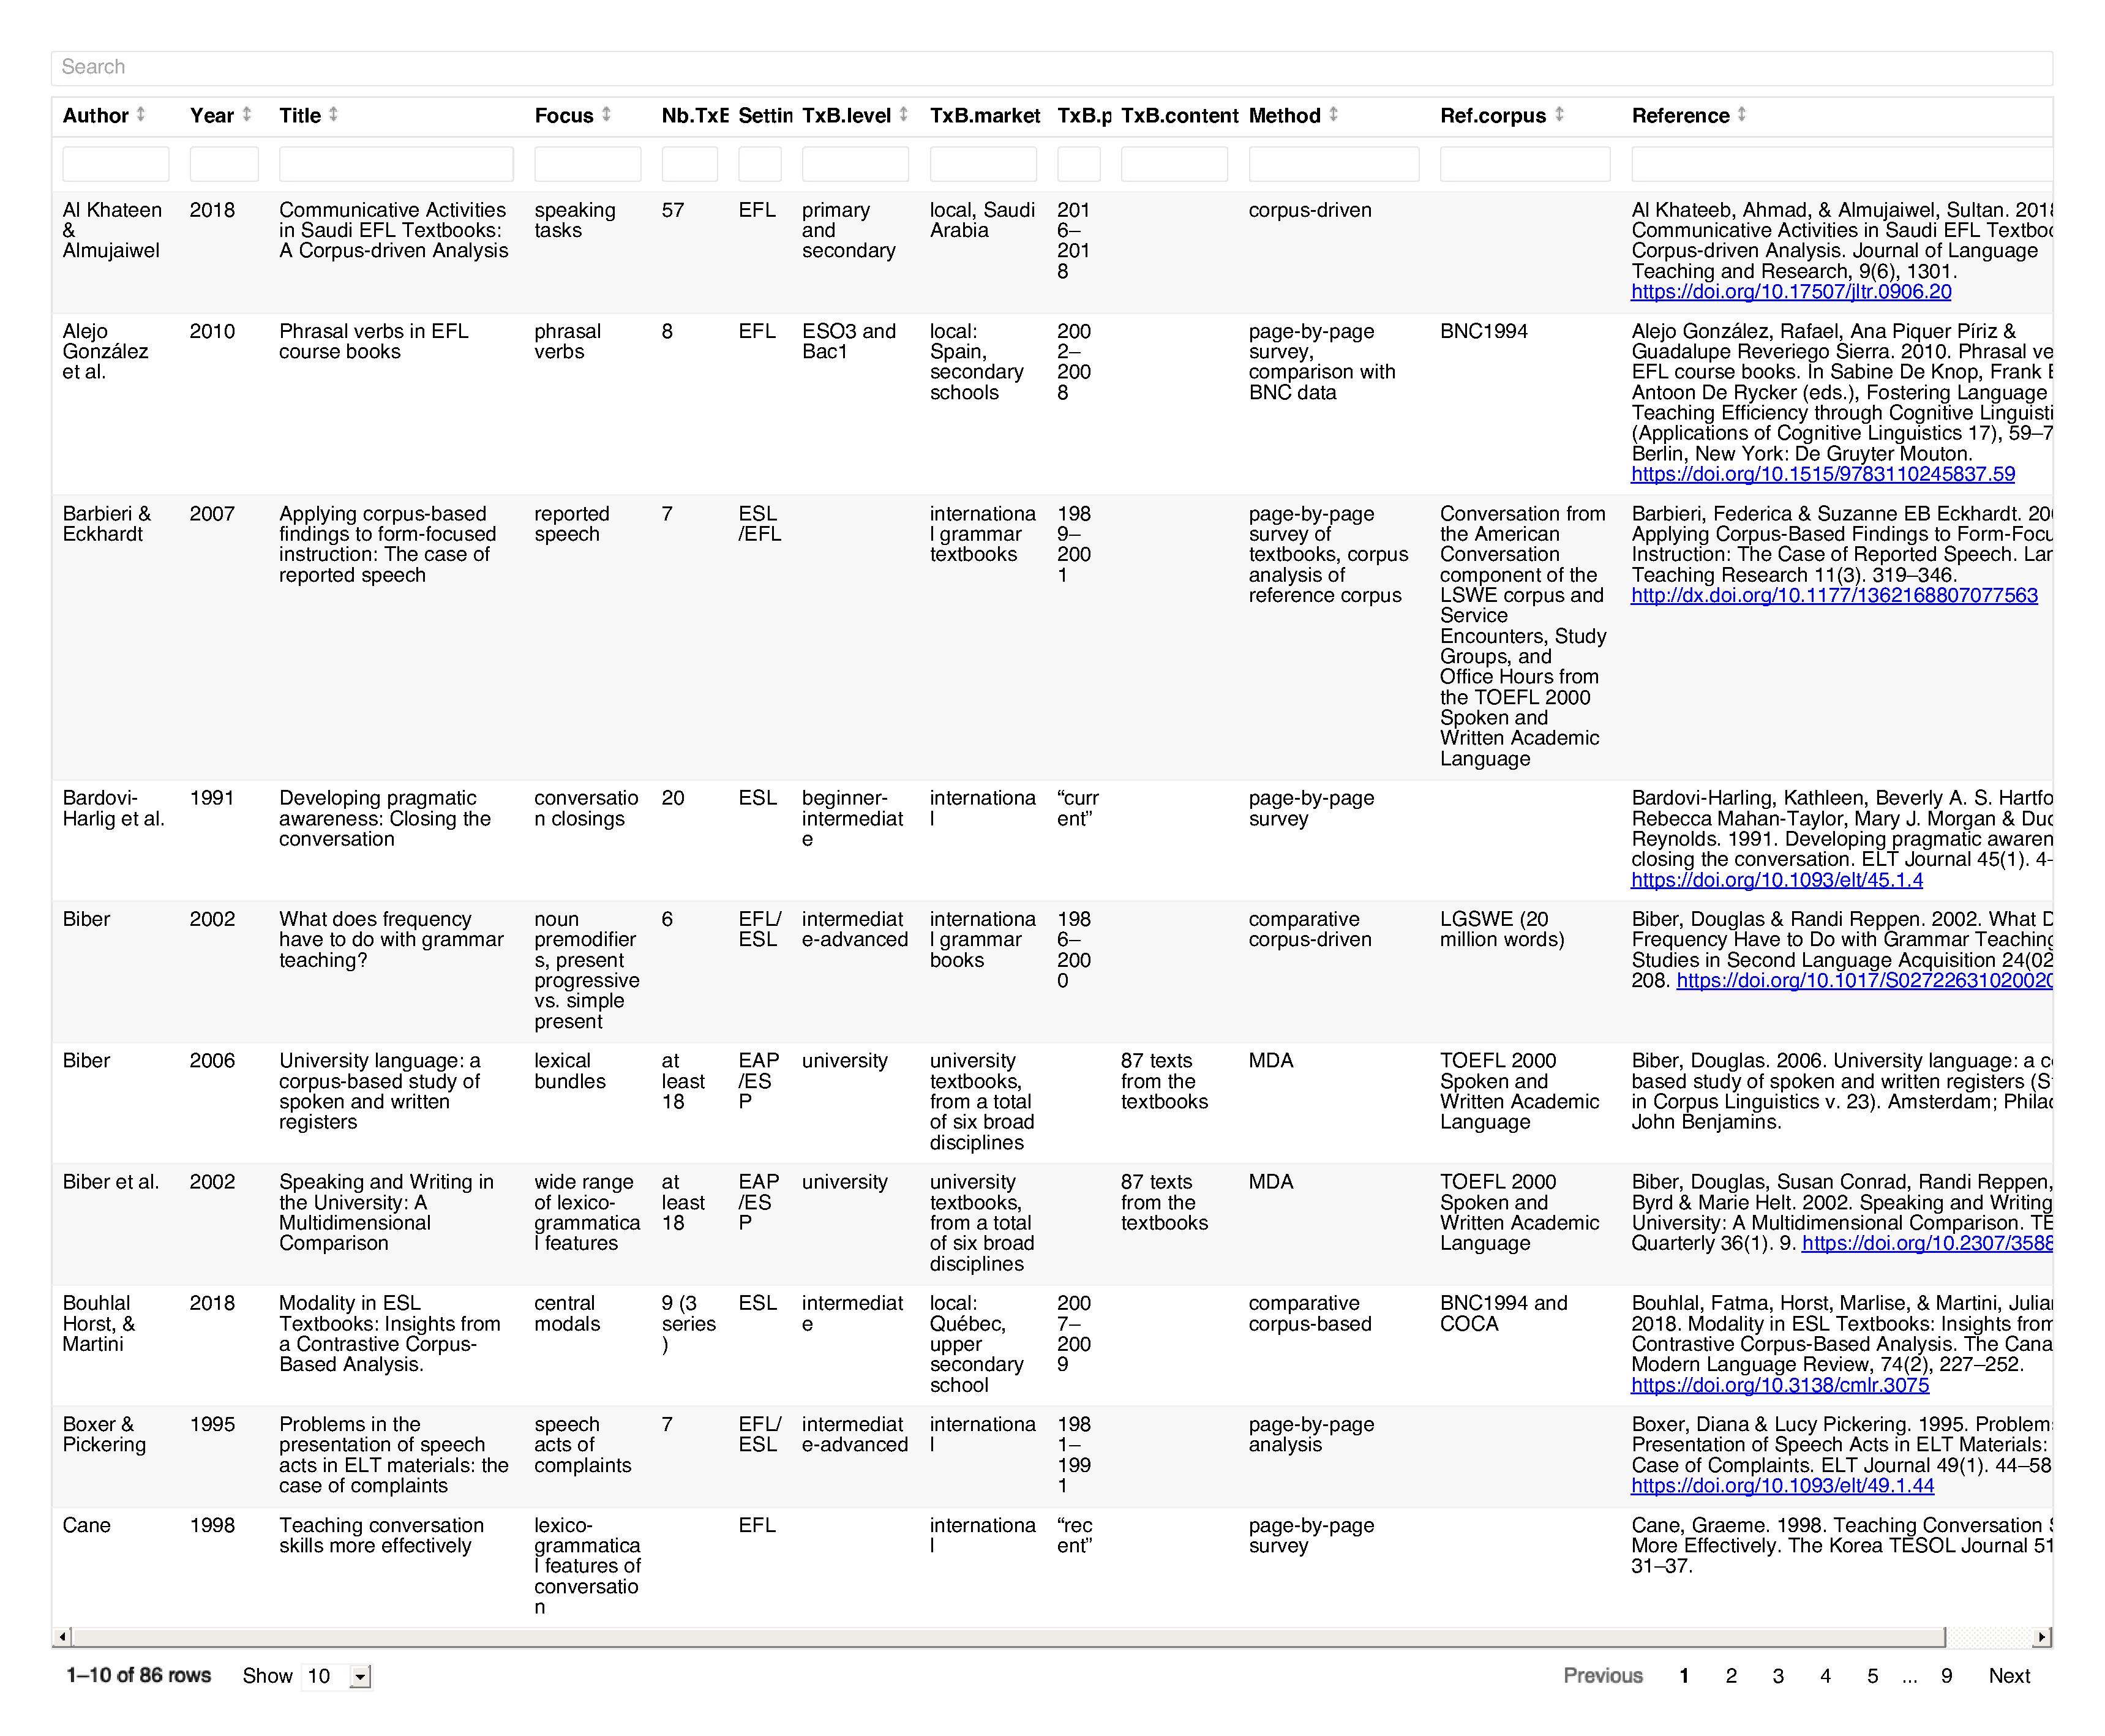
\includegraphics{A_LitReviewTable_files/figure-pdf/display-1.pdf}

The raw data can be downloaded as a comma-separated file from
\href{https://github.com/elenlefoll/TextbookMDA}{the project GitHub
repository}.

\chapter{Corpus data}\label{corpus-data}

\section{Textbook English Corpus
(TEC)}\label{textbook-english-corpus-tec}

A detailed tabular overview of the composition of the Textbook English
Corpus (TEC) together with the full bibliographic metadata is available
at
\href{https://doi.org/10.5281/zenodo.4922819}{doi.org/10.5281/zenodo.4922819}.

Note that, for copyright reasons, the corpus itself cannot be published.
If you are interested in using the corpus for non-commercial research
purposes and/or in a potential research collaboration, please get in
touch with me via \href{https://orcid.org/0000-0002-5839-8010}{e-mail}.

\section{Reference corpora}\label{reference-corpora}

\subsection{Spoken BNC2014}\label{spoken-bnc2014}

The original corpus files of the Spoken British National Corpus (BNC)
2014 (Love et al. 2017; Love et al. 2019) can be downloaded for free for
research purposes from:
\url{http://corpora.lancs.ac.uk/bnc2014/signup.php}. I used the untagged
XML version.

The R script used to pre-process the untagged XML files into the format
used in this study (the ``John and Jill in Ivybridge'' version with
added full stops at speaker turns, as explained in Section 4.3.2.2 of
the book) can be found here:
\url{https://github.com/elenlefoll/TextbookEnglish/blob/main/3_Data/BNCspoken_nomark-up_JackJill.R}

\subsection{Informative Texts for Teens Corpus (Info
Teens)}\label{informative-texts-for-teens-corpus-info-teens}

For copyright reasons, the corpus itself cannot be made available.
Details of its composition can be found in Section 4.3.2.5 of the book.
If you are interested in using this corpus for non-commercial research
purposes and/or in a potential research collaboration, please get in
touch with me via \href{https://orcid.org/0000-0002-5839-8010}{e-mail}.

\subsection{Youth Fiction corpus}\label{youth-fiction-corpus}

For copyright reasons, the corpus itself cannot be made available. The
corresponding metadata can be found here:
\url{https://github.com/elenlefoll/TextbookEnglish/blob/main/3_Data/3_Youth_Fiction_Index.csv}.
If you are interested in using this corpus for non-commercial research
purposes and/or in a potential research collaboration, please get in
touch with me via \href{https://orcid.org/0000-0002-5839-8010}{e-mail}.

\chapter{Data Preparation for the Model of Intra-Textbook
Variation}\label{data-preparation-for-the-model-of-intra-textbook-variation}

This script documents the steps taken to pre-process the Textbook
English Corpus (TEC) data that were entered in the multi-dimensional
model of intra-textbook linguistic variation (Chapter 6).

\section{Packages required}\label{packages-required}

The following packages must be installed and loaded to process the data.

\begin{Shaded}
\begin{Highlighting}[]
\CommentTok{\#renv::restore() \# Restore the project\textquotesingle{}s dependencies from the lockfile to ensure that same package versions are used as in the original study}

\FunctionTok{library}\NormalTok{(caret) }\CommentTok{\# For its confusion matrix function}
\FunctionTok{library}\NormalTok{(DT) }\CommentTok{\# To display interactive HTML tables}
\FunctionTok{library}\NormalTok{(here) }\CommentTok{\# For dynamic file paths}
\FunctionTok{library}\NormalTok{(knitr) }\CommentTok{\# Loaded to display the tables using the kable() function}
\FunctionTok{library}\NormalTok{(patchwork) }\CommentTok{\# Needed to put together Fig. 1}
\FunctionTok{library}\NormalTok{(PerformanceAnalytics) }\CommentTok{\# For the correlation plot}
\FunctionTok{library}\NormalTok{(psych) }\CommentTok{\# For various useful, stats function}
\FunctionTok{library}\NormalTok{(tidyverse) }\CommentTok{\# For data wrangling}
\end{Highlighting}
\end{Shaded}

\section{Data import from MFTE
output}\label{data-import-from-mfte-output}

The raw data used in this script is a tab-separated file that
corresponds to the tabular output of mixed normalised frequencies as
generated by the
\href{https://github.com/mshakirDr/MultiFeatureTaggerEnglish}{MFTE Perl
v. 3.1} (Le Foll 2021a).

\begin{Shaded}
\begin{Highlighting}[]
\CommentTok{\# Read in Textbook Corpus data}
\NormalTok{TxBcounts }\OtherTok{\textless{}{-}} \FunctionTok{read.delim}\NormalTok{(}\FunctionTok{here}\NormalTok{(}\StringTok{"data"}\NormalTok{, }\StringTok{"MFTE"}\NormalTok{, }\StringTok{"TxB900MDA\_3.1\_normed\_complex\_counts.tsv"}\NormalTok{), }\AttributeTok{header =} \ConstantTok{TRUE}\NormalTok{, }\AttributeTok{stringsAsFactors =} \ConstantTok{TRUE}\NormalTok{)}
\NormalTok{TxBcounts }\OtherTok{\textless{}{-}}\NormalTok{ TxBcounts }\SpecialCharTok{|\textgreater{}} 
  \FunctionTok{filter}\NormalTok{(Filename}\SpecialCharTok{!=}\StringTok{".DS\_Store"}\NormalTok{) }\SpecialCharTok{|\textgreater{}}  
  \FunctionTok{droplevels}\NormalTok{()}
\CommentTok{\#str(TxBcounts) \# Check sanity of data}
\CommentTok{\#nrow(TxBcounts) \# Should be 2014 files}
\FunctionTok{datatable}\NormalTok{(TxBcounts,}
  \AttributeTok{filter =} \StringTok{"top"}\NormalTok{,}
\NormalTok{) }\SpecialCharTok{|\textgreater{}} 
  \FunctionTok{formatRound}\NormalTok{(}\DecValTok{2}\SpecialCharTok{:}\FunctionTok{ncol}\NormalTok{(TxBcounts), }\AttributeTok{digits=}\DecValTok{2}\NormalTok{)}
\end{Highlighting}
\end{Shaded}


\includegraphics{D_Ch6_DataPrep_files/figure-pdf/raw_data-1.pdf}

Metadata was added on the basis of the filenames.

\begin{Shaded}
\begin{Highlighting}[]
\CommentTok{\# Adding a textbook proficiency level}
\NormalTok{TxBLevels }\OtherTok{\textless{}{-}} \FunctionTok{read.delim}\NormalTok{(}\FunctionTok{here}\NormalTok{(}\StringTok{"data"}\NormalTok{, }\StringTok{"metadata"}\NormalTok{, }\StringTok{"TxB900MDA\_ProficiencyLevels.csv"}\NormalTok{), }\AttributeTok{sep =} \StringTok{","}\NormalTok{)}
\NormalTok{TxBcounts }\OtherTok{\textless{}{-}} \FunctionTok{full\_join}\NormalTok{(TxBcounts, TxBLevels, }\AttributeTok{by =} \StringTok{"Filename"}\NormalTok{) }\SpecialCharTok{|\textgreater{}}  
  \FunctionTok{mutate}\NormalTok{(}\AttributeTok{Level =} \FunctionTok{as.factor}\NormalTok{(Level)) }\SpecialCharTok{|\textgreater{}}  
  \FunctionTok{mutate}\NormalTok{(}\AttributeTok{Filename =} \FunctionTok{as.factor}\NormalTok{(Filename))}

\CommentTok{\# Check distribution and that there are no NAs}
\FunctionTok{summary}\NormalTok{(TxBcounts}\SpecialCharTok{$}\NormalTok{Level) }\SpecialCharTok{|\textgreater{}} 
  \FunctionTok{kable}\NormalTok{(}\AttributeTok{col.names =} \FunctionTok{c}\NormalTok{(}\StringTok{"Textbook Level"}\NormalTok{, }\StringTok{"\# of texts"}\NormalTok{))}
\end{Highlighting}
\end{Shaded}

\begin{longtable}[]{@{}lr@{}}
\toprule\noalign{}
Textbook Level & \# of texts \\
\midrule\noalign{}
\endhead
\bottomrule\noalign{}
\endlastfoot
A & 292 \\
B & 407 \\
C & 506 \\
D & 478 \\
E & 331 \\
\end{longtable}

\begin{Shaded}
\begin{Highlighting}[]
\CommentTok{\# Check matching on random sample}
\CommentTok{\# TxBcounts |\textgreater{}}
\CommentTok{\#   select(Filename, Level) |\textgreater{}  }
\CommentTok{\#   sample\_n(20) }

\CommentTok{\# Adding a register variable from the file names}
\NormalTok{TxBcounts}\SpecialCharTok{$}\NormalTok{Register }\OtherTok{\textless{}{-}} \FunctionTok{as.factor}\NormalTok{(stringr}\SpecialCharTok{::}\FunctionTok{str\_extract}\NormalTok{(TxBcounts}\SpecialCharTok{$}\NormalTok{Filename, }\StringTok{"Spoken|Narrative|Other|Personal|Informative|Instructional|Poetry"}\NormalTok{)) }\CommentTok{\# Add a variable for Textbook Register}
\FunctionTok{summary}\NormalTok{(TxBcounts}\SpecialCharTok{$}\NormalTok{Register) }\SpecialCharTok{|\textgreater{}} 
  \FunctionTok{kable}\NormalTok{(}\AttributeTok{col.names =} \FunctionTok{c}\NormalTok{(}\StringTok{"Textbook Register"}\NormalTok{, }\StringTok{"\# of texts"}\NormalTok{))}
\end{Highlighting}
\end{Shaded}

\begin{longtable}[]{@{}lr@{}}
\toprule\noalign{}
Textbook Register & \# of texts \\
\midrule\noalign{}
\endhead
\bottomrule\noalign{}
\endlastfoot
Informative & 364 \\
Instructional & 647 \\
Narrative & 285 \\
Personal & 88 \\
Poetry & 37 \\
Spoken & 593 \\
\end{longtable}

\begin{Shaded}
\begin{Highlighting}[]
\NormalTok{TxBcounts}\SpecialCharTok{$}\NormalTok{Register }\OtherTok{\textless{}{-}}\NormalTok{ car}\SpecialCharTok{::}\FunctionTok{recode}\NormalTok{(TxBcounts}\SpecialCharTok{$}\NormalTok{Register, }\StringTok{"\textquotesingle{}Narrative\textquotesingle{} = \textquotesingle{}Fiction\textquotesingle{}; \textquotesingle{}Spoken\textquotesingle{} = \textquotesingle{}Conversation\textquotesingle{}"}\NormalTok{)}
\CommentTok{\#colnames(TxBcounts) \# Check all the variables make sense}

\CommentTok{\# Adding a textbook series variable from the file names}
\NormalTok{TxBcounts}\SpecialCharTok{$}\NormalTok{Filename }\OtherTok{\textless{}{-}}\NormalTok{ stringr}\SpecialCharTok{::}\FunctionTok{str\_replace}\NormalTok{(TxBcounts}\SpecialCharTok{$}\NormalTok{Filename, }\StringTok{"English\_In\_Mind|English\_in\_Mind"}\NormalTok{, }\StringTok{"EIM"}\NormalTok{) }
\NormalTok{TxBcounts}\SpecialCharTok{$}\NormalTok{Filename }\OtherTok{\textless{}{-}}\NormalTok{ stringr}\SpecialCharTok{::}\FunctionTok{str\_replace}\NormalTok{(TxBcounts}\SpecialCharTok{$}\NormalTok{Filename, }\StringTok{"New\_GreenLine"}\NormalTok{, }\StringTok{"NGL"}\NormalTok{) }\CommentTok{\# Otherwise the regex for GreenLine will override New\_GreenLine}
\NormalTok{TxBcounts}\SpecialCharTok{$}\NormalTok{Filename }\OtherTok{\textless{}{-}}\NormalTok{ stringr}\SpecialCharTok{::}\FunctionTok{str\_replace}\NormalTok{(TxBcounts}\SpecialCharTok{$}\NormalTok{Filename, }\StringTok{"Piece\_of\_cake"}\NormalTok{, }\StringTok{"POC"}\NormalTok{) }\CommentTok{\# Shorten label for ease of plotting}
\NormalTok{TxBcounts}\SpecialCharTok{$}\NormalTok{Series }\OtherTok{\textless{}{-}} \FunctionTok{as.factor}\NormalTok{(stringr}\SpecialCharTok{::}\FunctionTok{str\_extract}\NormalTok{(TxBcounts}\SpecialCharTok{$}\NormalTok{Filename, }\StringTok{"Access|Achievers|EIM|GreenLine|HT|NB|NM|POC|JTT|NGL|Solutions"}\NormalTok{)) }\CommentTok{\# Extract textbook series from (ammended) filenames}
\FunctionTok{summary}\NormalTok{(TxBcounts}\SpecialCharTok{$}\NormalTok{Series)  }\SpecialCharTok{|\textgreater{}} 
  \FunctionTok{kable}\NormalTok{(}\AttributeTok{col.names =} \FunctionTok{c}\NormalTok{(}\StringTok{"Textbook Name"}\NormalTok{, }\StringTok{"\# of texts"}\NormalTok{))}
\end{Highlighting}
\end{Shaded}

\begin{longtable}[]{@{}lr@{}}
\toprule\noalign{}
Textbook Name & \# of texts \\
\midrule\noalign{}
\endhead
\bottomrule\noalign{}
\endlastfoot
Access & 315 \\
Achievers & 240 \\
EIM & 180 \\
GreenLine & 209 \\
HT & 115 \\
JTT & 129 \\
NB & 44 \\
NGL & 298 \\
NM & 59 \\
POC & 98 \\
Solutions & 327 \\
\end{longtable}

\begin{Shaded}
\begin{Highlighting}[]
\CommentTok{\# Including the French textbooks for the first year of Lycée to their corresponding publisher series from collège}
\NormalTok{TxBcounts}\SpecialCharTok{$}\NormalTok{Series }\OtherTok{\textless{}{-}}\NormalTok{car}\SpecialCharTok{::}\FunctionTok{recode}\NormalTok{(TxBcounts}\SpecialCharTok{$}\NormalTok{Series, }\StringTok{"c(\textquotesingle{}NB\textquotesingle{}, \textquotesingle{}JTT\textquotesingle{}) = \textquotesingle{}JTT\textquotesingle{}; c(\textquotesingle{}NM\textquotesingle{}, \textquotesingle{}HT\textquotesingle{}) = \textquotesingle{}HT\textquotesingle{}"}\NormalTok{) }\CommentTok{\# Recode final volumes of French series (see Section 4.3.1.1 on textbook selection for details)}
\FunctionTok{summary}\NormalTok{(TxBcounts}\SpecialCharTok{$}\NormalTok{Series) }\SpecialCharTok{|\textgreater{}} 
  \FunctionTok{kable}\NormalTok{(}\AttributeTok{col.names =} \FunctionTok{c}\NormalTok{(}\StringTok{"Textbook Series"}\NormalTok{, }\StringTok{"\# of texts"}\NormalTok{))}
\end{Highlighting}
\end{Shaded}

\begin{longtable}[]{@{}lr@{}}
\toprule\noalign{}
Textbook Series & \# of texts \\
\midrule\noalign{}
\endhead
\bottomrule\noalign{}
\endlastfoot
Access & 315 \\
Achievers & 240 \\
EIM & 180 \\
GreenLine & 209 \\
HT & 174 \\
JTT & 173 \\
NGL & 298 \\
POC & 98 \\
Solutions & 327 \\
\end{longtable}

\begin{Shaded}
\begin{Highlighting}[]
\CommentTok{\# Adding a textbook country of use variable from the series variable}
\NormalTok{TxBcounts}\SpecialCharTok{$}\NormalTok{Country }\OtherTok{\textless{}{-}}\NormalTok{ TxBcounts}\SpecialCharTok{$}\NormalTok{Series}
\NormalTok{TxBcounts}\SpecialCharTok{$}\NormalTok{Country }\OtherTok{\textless{}{-}}\NormalTok{ car}\SpecialCharTok{::}\FunctionTok{recode}\NormalTok{(TxBcounts}\SpecialCharTok{$}\NormalTok{Series, }\StringTok{"c(\textquotesingle{}Access\textquotesingle{}, \textquotesingle{}GreenLine\textquotesingle{}, \textquotesingle{}NGL\textquotesingle{}) = \textquotesingle{}Germany\textquotesingle{}; c(\textquotesingle{}Achievers\textquotesingle{}, \textquotesingle{}EIM\textquotesingle{}, \textquotesingle{}Solutions\textquotesingle{}) = \textquotesingle{}Spain\textquotesingle{}; c(\textquotesingle{}HT\textquotesingle{}, \textquotesingle{}NB\textquotesingle{}, \textquotesingle{}NM\textquotesingle{}, \textquotesingle{}POC\textquotesingle{}, \textquotesingle{}JTT\textquotesingle{}) = \textquotesingle{}France\textquotesingle{}"}\NormalTok{)}
\FunctionTok{summary}\NormalTok{(TxBcounts}\SpecialCharTok{$}\NormalTok{Country) }\SpecialCharTok{|\textgreater{}} 
  \FunctionTok{kable}\NormalTok{(}\AttributeTok{col.names =} \FunctionTok{c}\NormalTok{(}\StringTok{"Country of Use"}\NormalTok{, }\StringTok{"\# of texts"}\NormalTok{))}
\end{Highlighting}
\end{Shaded}

\begin{longtable}[]{@{}lr@{}}
\toprule\noalign{}
Country of Use & \# of texts \\
\midrule\noalign{}
\endhead
\bottomrule\noalign{}
\endlastfoot
France & 445 \\
Germany & 822 \\
Spain & 747 \\
\end{longtable}

\begin{Shaded}
\begin{Highlighting}[]
\CommentTok{\# Re{-}order variables}
\CommentTok{\#colnames(TxBcounts)}
\NormalTok{TxBcounts }\OtherTok{\textless{}{-}} \FunctionTok{select}\NormalTok{(TxBcounts, }\FunctionTok{order}\NormalTok{(}\FunctionTok{names}\NormalTok{(TxBcounts))) }\SpecialCharTok{\%\textgreater{}\%}
  \FunctionTok{select}\NormalTok{(Filename, Country, Series, Level, Register, Words, }\FunctionTok{everything}\NormalTok{())}
\CommentTok{\#colnames(TxBcounts)}
\end{Highlighting}
\end{Shaded}

\subsection{Corpus size}\label{corpus-size}

This table provides some summary statistics about the number of words
included in the TEC texts originally tagged for this study.

\begin{Shaded}
\begin{Highlighting}[]
\NormalTok{TxBcounts  }\SpecialCharTok{|\textgreater{}}  
  \FunctionTok{group\_by}\NormalTok{(Register) }\SpecialCharTok{|\textgreater{}}  
  \FunctionTok{summarise}\NormalTok{(}\AttributeTok{totaltexts =} \FunctionTok{n}\NormalTok{(), }\AttributeTok{totalwords =} \FunctionTok{sum}\NormalTok{(Words), }\AttributeTok{mean =} \FunctionTok{as.integer}\NormalTok{(}\FunctionTok{mean}\NormalTok{(Words)), }\AttributeTok{sd =} \FunctionTok{as.integer}\NormalTok{(}\FunctionTok{sd}\NormalTok{(Words)), }\AttributeTok{TTRmean =} \FunctionTok{mean}\NormalTok{(TTR)) }\SpecialCharTok{|\textgreater{}}  
  \FunctionTok{kable}\NormalTok{(}\AttributeTok{digits =} \DecValTok{2}\NormalTok{, }\AttributeTok{format.args =} \FunctionTok{list}\NormalTok{(}\AttributeTok{big.mark =} \StringTok{","}\NormalTok{))}
\end{Highlighting}
\end{Shaded}

\begin{longtable}[]{@{}lrrrrr@{}}
\toprule\noalign{}
Register & totaltexts & totalwords & mean & sd & TTRmean \\
\midrule\noalign{}
\endhead
\bottomrule\noalign{}
\endlastfoot
Conversation & 593 & 505,147 & 851 & 301 & 0.44 \\
Fiction & 285 & 241,512 & 847 & 208 & 0.47 \\
Informative & 364 & 304,695 & 837 & 177 & 0.51 \\
Instructional & 647 & 585,049 & 904 & 94 & 0.42 \\
Personal & 88 & 69,570 & 790 & 177 & 0.48 \\
Poetry & 37 & 26,445 & 714 & 192 & 0.44 \\
\end{longtable}

\begin{Shaded}
\begin{Highlighting}[]
\CommentTok{\#TxBcounts \textless{}{-} saveRDS(TxBcounts, here("data", "processed", "TxBcounts.rds"))}
\end{Highlighting}
\end{Shaded}

\section{Data preparation for PCA}\label{data-preparation-for-pca}

Poetry texts were removed for this analysis as there were too few
compared to the other register categories.

\begin{Shaded}
\begin{Highlighting}[]
\FunctionTok{summary}\NormalTok{(TxBcounts}\SpecialCharTok{$}\NormalTok{Register) }\SpecialCharTok{|\textgreater{}}  
  \FunctionTok{kable}\NormalTok{(}\AttributeTok{col.names =} \FunctionTok{c}\NormalTok{(}\StringTok{"Register"}\NormalTok{, }\StringTok{"\# texts"}\NormalTok{))}
\end{Highlighting}
\end{Shaded}

\begin{longtable}[]{@{}lr@{}}
\toprule\noalign{}
Register & \# texts \\
\midrule\noalign{}
\endhead
\bottomrule\noalign{}
\endlastfoot
Conversation & 593 \\
Fiction & 285 \\
Informative & 364 \\
Instructional & 647 \\
Personal & 88 \\
Poetry & 37 \\
\end{longtable}

This led to the following distribution of texts across the five textbook
English registers examined in the model of intra-textbook linguistic
variation:

\begin{Shaded}
\begin{Highlighting}[]
\NormalTok{TxBcounts }\OtherTok{\textless{}{-}}\NormalTok{ TxBcounts }\SpecialCharTok{|\textgreater{}}  
  \FunctionTok{filter}\NormalTok{(Register}\SpecialCharTok{!=}\StringTok{"Poetry"}\NormalTok{) }\SpecialCharTok{|\textgreater{}}  
  \FunctionTok{droplevels}\NormalTok{()}

\FunctionTok{summary}\NormalTok{(TxBcounts}\SpecialCharTok{$}\NormalTok{Register) }\SpecialCharTok{|\textgreater{}}  
  \FunctionTok{kable}\NormalTok{(}\AttributeTok{col.names =} \FunctionTok{c}\NormalTok{(}\StringTok{"Register"}\NormalTok{, }\StringTok{"\# texts"}\NormalTok{))}
\end{Highlighting}
\end{Shaded}

\begin{longtable}[]{@{}lr@{}}
\toprule\noalign{}
Register & \# texts \\
\midrule\noalign{}
\endhead
\bottomrule\noalign{}
\endlastfoot
Conversation & 593 \\
Fiction & 285 \\
Informative & 364 \\
Instructional & 647 \\
Personal & 88 \\
\end{longtable}

\subsection{Feature distributions}\label{feature-distributions}

The distributions of each linguistic features were examined by means of
visualisation. As shown below, before transformation, many of the
features displayed highly skewed distributions.

\begin{Shaded}
\begin{Highlighting}[]
\NormalTok{TxBcounts }\SpecialCharTok{|\textgreater{}} 
  \FunctionTok{select}\NormalTok{(}\SpecialCharTok{{-}}\NormalTok{Words) }\SpecialCharTok{|\textgreater{}}  
  \FunctionTok{keep}\NormalTok{(is.numeric) }\SpecialCharTok{|\textgreater{}}  
\NormalTok{  tidyr}\SpecialCharTok{::}\FunctionTok{gather}\NormalTok{() }\SpecialCharTok{|\textgreater{}}  \CommentTok{\# This function from tidyr converts a selection of variables into two variables: a key and a value. The key contains the names of the original variable and the value the data. This means we can then use the facet\_wrap function from ggplot2}
  \FunctionTok{ggplot}\NormalTok{(}\FunctionTok{aes}\NormalTok{(value)) }\SpecialCharTok{+}
    \FunctionTok{theme\_bw}\NormalTok{() }\SpecialCharTok{+}
    \FunctionTok{facet\_wrap}\NormalTok{(}\SpecialCharTok{\textasciitilde{}}\NormalTok{ key, }\AttributeTok{scales =} \StringTok{"free"}\NormalTok{, }\AttributeTok{ncol =} \DecValTok{4}\NormalTok{) }\SpecialCharTok{+}
    \FunctionTok{scale\_x\_continuous}\NormalTok{(}\AttributeTok{expand=}\FunctionTok{c}\NormalTok{(}\DecValTok{0}\NormalTok{,}\DecValTok{0}\NormalTok{)) }\SpecialCharTok{+}
    \FunctionTok{geom\_histogram}\NormalTok{(}\AttributeTok{bins =} \DecValTok{30}\NormalTok{, }\AttributeTok{colour=} \StringTok{"darkred"}\NormalTok{, }\AttributeTok{fill =} \StringTok{"darkred"}\NormalTok{, }\AttributeTok{alpha =} \FloatTok{0.5}\NormalTok{)}
\end{Highlighting}
\end{Shaded}

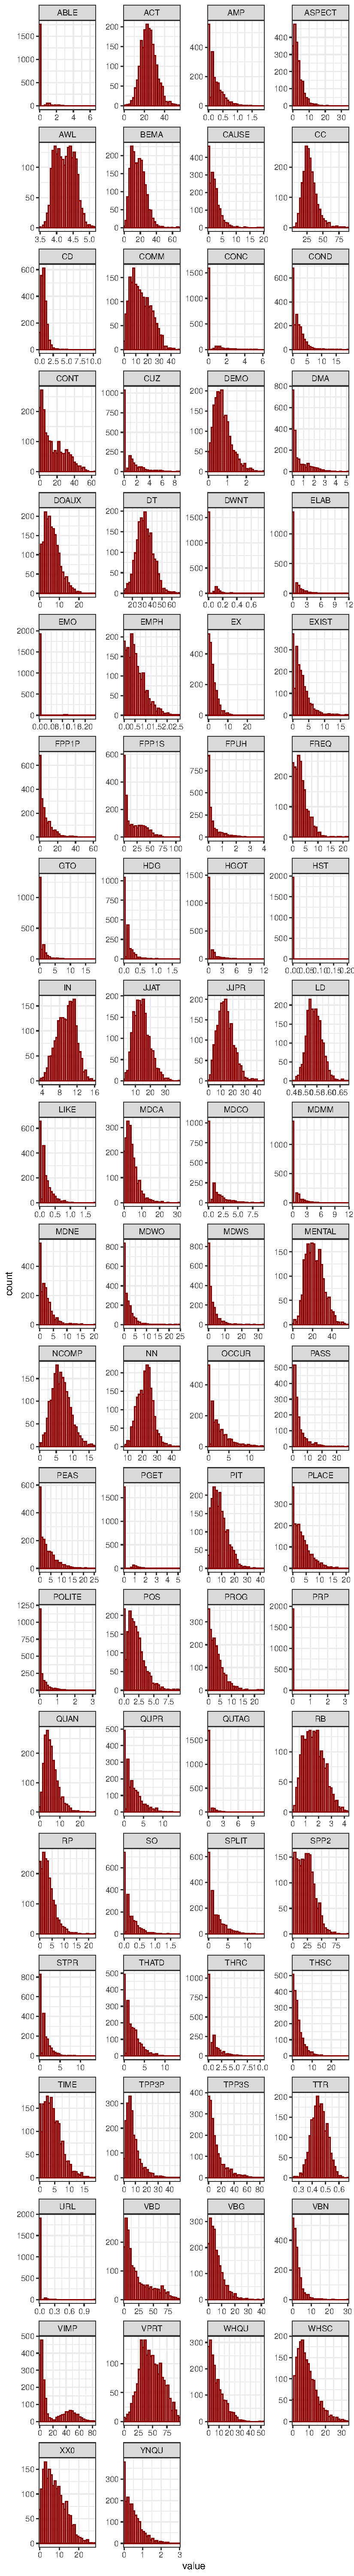
\includegraphics{D_Ch6_DataPrep_files/figure-pdf/distribution-viz-1.pdf}

\begin{Shaded}
\begin{Highlighting}[]
\CommentTok{\#ggsave(here("plots", "TEC{-}HistogramPlotsAllVariablesTEC{-}only.svg"), width = 20, height = 45)}
\end{Highlighting}
\end{Shaded}

\subsection{Feature removal}\label{feature-removal}

A number of features were removed from the dataset as they are not
linguistically interpretable. In the case of the TEC, this included the
variable CD because numbers spelt out as digits were removed from the
textbooks before these were tagged with the MFTE. In addition, the
variables LIKE and SO because these are ``bin'' features included in the
output of the MFTE to ensure that the counts for these polysemous words
do not inflate other categories due to mistags (Le Foll 2021b).

Whenever linguistically meaningful, very low-frequency features were
merged. Finally, features absent from more than third of texts were also
excluded. For the analysis intra-textbook register variation, the
following linguistic features were excluded from the analysis due to low
dispersion:

\begin{Shaded}
\begin{Highlighting}[]
\CommentTok{\# Removal of meaningless features:}
\NormalTok{TxBcounts }\OtherTok{\textless{}{-}}\NormalTok{ TxBcounts }\SpecialCharTok{|\textgreater{}}  
  \FunctionTok{select}\NormalTok{(}\SpecialCharTok{{-}}\FunctionTok{c}\NormalTok{(CD, LIKE, SO))}

\CommentTok{\# Function to compute percentage of texts with occurrences meeting a condition}
\NormalTok{compute\_percentage }\OtherTok{\textless{}{-}} \ControlFlowTok{function}\NormalTok{(data, condition, threshold) \{}
\NormalTok{  numeric\_data }\OtherTok{\textless{}{-}} \FunctionTok{Filter}\NormalTok{(is.numeric, data)}
\NormalTok{  percentage }\OtherTok{\textless{}{-}} \FunctionTok{round}\NormalTok{(}\FunctionTok{colSums}\NormalTok{(condition[, }\FunctionTok{sapply}\NormalTok{(numeric\_data, is.numeric)])}\SpecialCharTok{/}\FunctionTok{nrow}\NormalTok{(data) }\SpecialCharTok{*} \DecValTok{100}\NormalTok{, }\DecValTok{2}\NormalTok{)}
\NormalTok{  percentage }\OtherTok{\textless{}{-}} \FunctionTok{as.data.frame}\NormalTok{(percentage)}
  \FunctionTok{colnames}\NormalTok{(percentage) }\OtherTok{\textless{}{-}} \StringTok{"Percentage"}
\NormalTok{  percentage }\OtherTok{\textless{}{-}}\NormalTok{ percentage }\SpecialCharTok{|\textgreater{}}  
    \FunctionTok{filter}\NormalTok{(}\SpecialCharTok{!}\FunctionTok{is.na}\NormalTok{(Percentage)) }\SpecialCharTok{|\textgreater{}} 
    \FunctionTok{rownames\_to\_column}\NormalTok{() }\SpecialCharTok{|\textgreater{}} 
    \FunctionTok{arrange}\NormalTok{(Percentage)}
  \ControlFlowTok{if}\NormalTok{ (}\SpecialCharTok{!}\FunctionTok{missing}\NormalTok{(threshold)) \{}
\NormalTok{    percentage }\OtherTok{\textless{}{-}}\NormalTok{ percentage }\SpecialCharTok{|\textgreater{}}  
      \FunctionTok{filter}\NormalTok{(Percentage }\SpecialCharTok{\textgreater{}}\NormalTok{ threshold)}
\NormalTok{  \}}
  \FunctionTok{return}\NormalTok{(percentage)}
\NormalTok{\}}

\CommentTok{\# Calculate percentage of texts with 0 occurrences of each feature}
\NormalTok{zero\_features }\OtherTok{\textless{}{-}} \FunctionTok{compute\_percentage}\NormalTok{(TxBcounts, TxBcounts }\SpecialCharTok{==} \DecValTok{0}\NormalTok{, }\FloatTok{66.6}\NormalTok{)}
\CommentTok{\# zero\_features |\textgreater{} }
\CommentTok{\#   kable(col.names = c("Feature", "\% texts with zero occurrences"))}

\CommentTok{\# Combine low frequency features into meaningful groups whenever this makes linguistic sense}
\NormalTok{TxBcounts }\OtherTok{\textless{}{-}}\NormalTok{ TxBcounts }\SpecialCharTok{|\textgreater{}}  
  \FunctionTok{mutate}\NormalTok{(}\AttributeTok{JJPR =}\NormalTok{ ABLE }\SpecialCharTok{+}\NormalTok{ JJPR, }\AttributeTok{ABLE =} \ConstantTok{NULL}\NormalTok{) }\SpecialCharTok{|\textgreater{}}  
  \FunctionTok{mutate}\NormalTok{(}\AttributeTok{PASS =}\NormalTok{ PGET }\SpecialCharTok{+}\NormalTok{ PASS, }\AttributeTok{PGET =} \ConstantTok{NULL}\NormalTok{)}

\CommentTok{\# Re{-}calculate percentage of texts with 0 occurrences of each feature}
\NormalTok{zero\_features2 }\OtherTok{\textless{}{-}} \FunctionTok{compute\_percentage}\NormalTok{(TxBcounts, TxBcounts }\SpecialCharTok{==} \DecValTok{0}\NormalTok{, }\FloatTok{66.6}\NormalTok{)}
\NormalTok{zero\_features2 }\SpecialCharTok{|\textgreater{}} 
  \FunctionTok{kable}\NormalTok{(}\AttributeTok{col.names =} \FunctionTok{c}\NormalTok{(}\StringTok{"Feature"}\NormalTok{, }\StringTok{"\% texts with zero occurrences"}\NormalTok{))}
\end{Highlighting}
\end{Shaded}

\begin{longtable}[]{@{}lr@{}}
\toprule\noalign{}
Feature & \% texts with zero occurrences \\
\midrule\noalign{}
\endhead
\bottomrule\noalign{}
\endlastfoot
GTO & 67.07 \\
ELAB & 69.30 \\
MDMM & 70.81 \\
HGOT & 73.75 \\
CONC & 80.48 \\
DWNT & 81.44 \\
QUTAG & 85.99 \\
URL & 96.51 \\
EMO & 97.82 \\
PRP & 98.33 \\
HST & 99.44 \\
\end{longtable}

\begin{Shaded}
\begin{Highlighting}[]
\CommentTok{\# Drop variables with low document frequency}
\NormalTok{TxBcounts }\OtherTok{\textless{}{-}} \FunctionTok{select}\NormalTok{(TxBcounts, }\SpecialCharTok{{-}}\FunctionTok{one\_of}\NormalTok{(zero\_features2}\SpecialCharTok{$}\NormalTok{rowname))}
\CommentTok{\#ncol(TxBcounts){-}8 \# Number of linguistic features remaining}

\CommentTok{\# List of features}
\CommentTok{\#colnames(TxBcounts)}
\end{Highlighting}
\end{Shaded}

These feature removal operations resulted in a feature set of 64
linguistic variables.

\subsection{Identifying potential outlier
texts}\label{identifying-potential-outlier-texts}

All normalised frequencies were normalised to identify any potential
outlier texts.

\begin{Shaded}
\begin{Highlighting}[]
\NormalTok{TxBzcounts }\OtherTok{\textless{}{-}}\NormalTok{ TxBcounts }\SpecialCharTok{|\textgreater{}} 
  \FunctionTok{select}\NormalTok{(}\SpecialCharTok{{-}}\NormalTok{Words) }\SpecialCharTok{|\textgreater{}}  
  \FunctionTok{keep}\NormalTok{(is.numeric) }\SpecialCharTok{|\textgreater{}}  
  \FunctionTok{scale}\NormalTok{()}

\FunctionTok{boxplot}\NormalTok{(TxBzcounts, }\AttributeTok{las =} \DecValTok{3}\NormalTok{, }\AttributeTok{main =} \StringTok{"z{-}scores"}\NormalTok{) }\CommentTok{\# Slow to open!}
\end{Highlighting}
\end{Shaded}

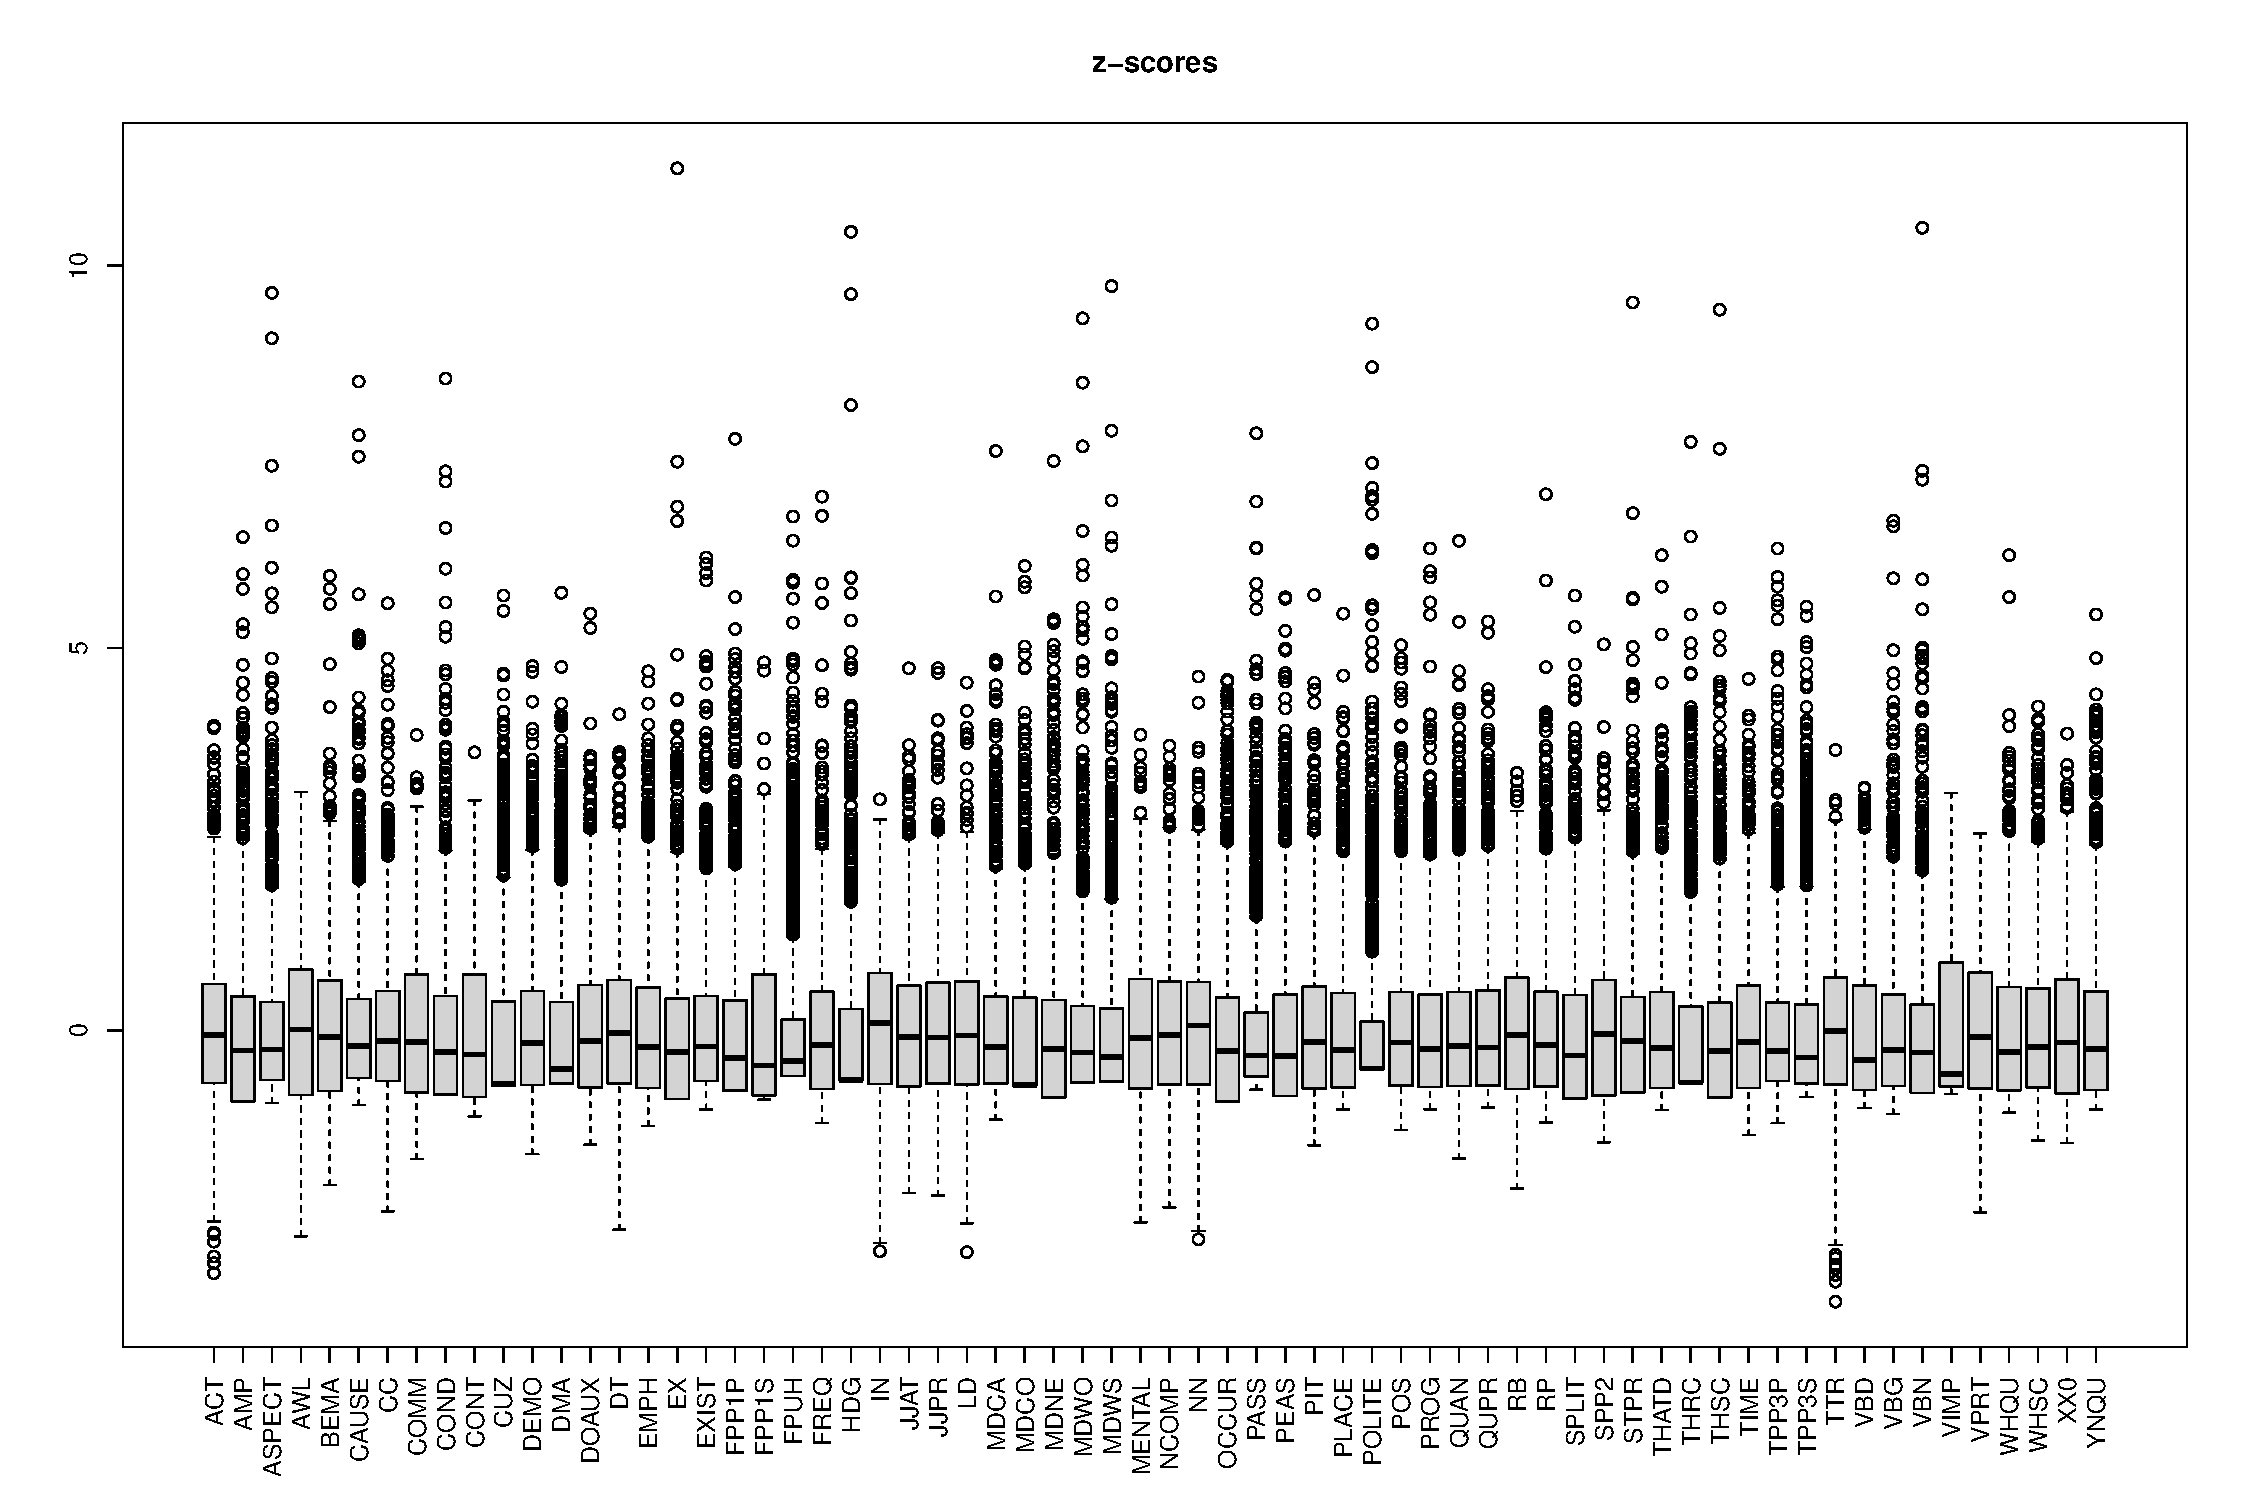
\includegraphics{D_Ch6_DataPrep_files/figure-pdf/z-standardisation-outliers-1.pdf}

\begin{Shaded}
\begin{Highlighting}[]
\CommentTok{\# If necessary, remove any outliers at this stage.}
\NormalTok{TxBdata }\OtherTok{\textless{}{-}} \FunctionTok{cbind}\NormalTok{(TxBcounts[,}\DecValTok{1}\SpecialCharTok{:}\DecValTok{6}\NormalTok{], }\FunctionTok{as.data.frame}\NormalTok{(TxBzcounts))}

\NormalTok{outliers }\OtherTok{\textless{}{-}}\NormalTok{ TxBdata }\SpecialCharTok{|\textgreater{}}  
  \FunctionTok{select}\NormalTok{(}\SpecialCharTok{{-}}\FunctionTok{c}\NormalTok{(Words, LD, TTR)) }\SpecialCharTok{|\textgreater{}}  
  \FunctionTok{filter}\NormalTok{(}\FunctionTok{if\_any}\NormalTok{(}\FunctionTok{where}\NormalTok{(is.numeric), }\SpecialCharTok{\textasciitilde{}}\NormalTok{ .x }\SpecialCharTok{\textgreater{}} \DecValTok{8}\NormalTok{)) }\SpecialCharTok{|\textgreater{}}  
  \FunctionTok{select}\NormalTok{(Filename)}
\end{Highlighting}
\end{Shaded}

The following outlier texts were identified and excluded in subsequent
analyses.

\begin{Shaded}
\begin{Highlighting}[]
\NormalTok{outliers}
\end{Highlighting}
\end{Shaded}

\begin{verbatim}
                                            Filename
1                             POC_4e_Spoken_0007.txt
2             Solutions_Elementary_Personal_0001.txt
3                       NGL_5_Instructional_0018.txt
4                           Access_1_Spoken_0011.txt
5                              EIM_1_Spoken_0012.txt
6                              NGL_4_Spoken_0011.txt
7      Solutions_Intermediate_Plus_Personal_0001.txt
8           Solutions_Elementary_ELF_Spoken_0021.txt
9                          NB_2_Informative_0009.txt
10       Solutions_Intermediate_Plus_Spoken_0022.txt
11     Solutions_Intermediate_Instructional_0025.txt
12 Solutions_Pre-Intermediate_Instructional_0024.txt
13                            POC_4e_Spoken_0010.txt
14            Solutions_Intermediate_Spoken_0019.txt
15                          Access_1_Spoken_0019.txt
16    Solutions_Pre-Intermediate_ELF_Spoken_0005.txt
\end{verbatim}

\begin{Shaded}
\begin{Highlighting}[]
\NormalTok{TxBcounts }\OtherTok{\textless{}{-}}\NormalTok{ TxBcounts }\SpecialCharTok{|\textgreater{}}  
  \FunctionTok{filter}\NormalTok{(}\SpecialCharTok{!}\NormalTok{Filename }\SpecialCharTok{\%in\%}\NormalTok{ outliers}\SpecialCharTok{$}\NormalTok{Filename)}

\CommentTok{\#saveRDS(TxBcounts, here("data", "processed", "TxBcounts3.rds")) \# Last saved 6 March 2024}

\NormalTok{TxBzcounts }\OtherTok{\textless{}{-}}\NormalTok{ TxBcounts }\SpecialCharTok{|\textgreater{}} 
  \FunctionTok{select}\NormalTok{(}\SpecialCharTok{{-}}\NormalTok{Words) }\SpecialCharTok{|\textgreater{}}  
  \FunctionTok{keep}\NormalTok{(is.numeric) }\SpecialCharTok{|\textgreater{}}  
  \FunctionTok{scale}\NormalTok{()}
\end{Highlighting}
\end{Shaded}

This resulted in 1,961 TEC texts being included in the model of
intra-textbook linguistic variation with the following standardised
feature distributions.

\begin{Shaded}
\begin{Highlighting}[]
\NormalTok{TxBzcounts }\SpecialCharTok{|\textgreater{}} 
  \FunctionTok{as.data.frame}\NormalTok{() }\SpecialCharTok{|\textgreater{}}  
  \FunctionTok{gather}\NormalTok{() }\SpecialCharTok{|\textgreater{}}  \CommentTok{\# This function from tidyr converts a selection of variables into two variables: a key and a value. The key contains the names of the original variable and the value the data. This means we can then use the facet\_wrap function from ggplot2}
  \FunctionTok{ggplot}\NormalTok{(}\FunctionTok{aes}\NormalTok{(value)) }\SpecialCharTok{+}
    \FunctionTok{theme\_bw}\NormalTok{() }\SpecialCharTok{+}
    \FunctionTok{facet\_wrap}\NormalTok{(}\SpecialCharTok{\textasciitilde{}}\NormalTok{ key, }\AttributeTok{scales =} \StringTok{"free"}\NormalTok{, }\AttributeTok{ncol =} \DecValTok{4}\NormalTok{) }\SpecialCharTok{+}
    \FunctionTok{scale\_x\_continuous}\NormalTok{(}\AttributeTok{expand=}\FunctionTok{c}\NormalTok{(}\DecValTok{0}\NormalTok{,}\DecValTok{0}\NormalTok{)) }\SpecialCharTok{+}
    \FunctionTok{geom\_histogram}\NormalTok{(}\AttributeTok{bins =} \DecValTok{30}\NormalTok{, }\AttributeTok{colour=} \StringTok{"darkred"}\NormalTok{, }\AttributeTok{fill =} \StringTok{"darkred"}\NormalTok{, }\AttributeTok{alpha =} \FloatTok{0.5}\NormalTok{)}
\end{Highlighting}
\end{Shaded}

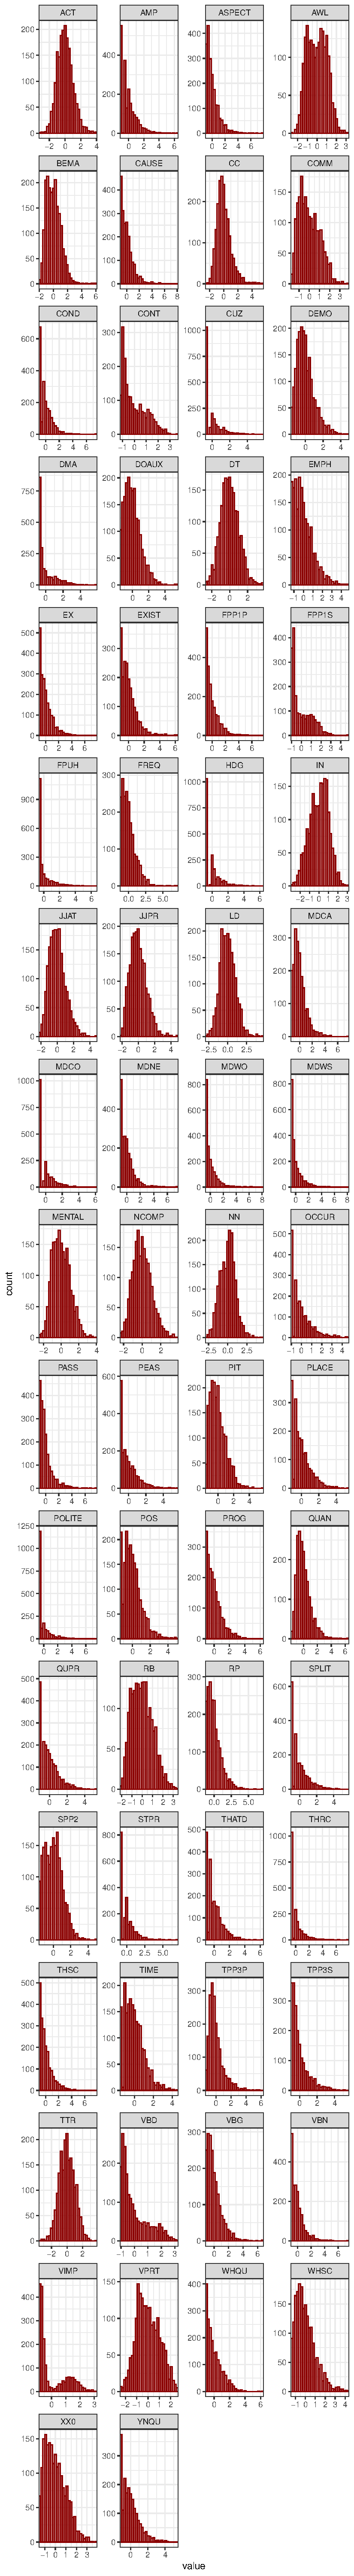
\includegraphics{D_Ch6_DataPrep_files/figure-pdf/z-transformed-distributions-1.pdf}

\begin{Shaded}
\begin{Highlighting}[]
\CommentTok{\#ggsave(here("plots", "TEC{-}zscores{-}HistogramsAllVariablesTEC{-}only.svg"), width = 20, height = 45)}
\end{Highlighting}
\end{Shaded}

\subsection{Signed log transformation}\label{signed-log-transformation}

A signed logarithmic transformation was applied to (further) deskew the
feature distributions (Diwersy, Evert, and Neumann 2014; Neumann and
Evert 2021).

The signed log transformation function was inspired by the SignedLog
function proposed in
https://cran.r-project.org/web/packages/DataVisualizations/DataVisualizations.pdf

\begin{Shaded}
\begin{Highlighting}[]
\CommentTok{\# All features are signed log{-}transformed (note that this is also what Neumann \& Evert 2021 propose)}
\NormalTok{signed.log }\OtherTok{\textless{}{-}} \ControlFlowTok{function}\NormalTok{(x) \{}
  \FunctionTok{sign}\NormalTok{(x) }\SpecialCharTok{*} \FunctionTok{log}\NormalTok{(}\FunctionTok{abs}\NormalTok{(x) }\SpecialCharTok{+} \DecValTok{1}\NormalTok{)}
\NormalTok{  \}}

\NormalTok{TxBzlogcounts }\OtherTok{\textless{}{-}} \FunctionTok{signed.log}\NormalTok{(TxBzcounts) }\CommentTok{\# Standardise first, then signed log transform}

\CommentTok{\#saveRDS(TxBzlogcounts, here("data", "processed", "TxBzlogcounts.rds")) \# Last saved 6 March 2024}
\end{Highlighting}
\end{Shaded}

The new feature distributions are visualised below.

\begin{Shaded}
\begin{Highlighting}[]
\NormalTok{TxBzlogcounts }\SpecialCharTok{|\textgreater{}} 
  \FunctionTok{as.data.frame}\NormalTok{() }\SpecialCharTok{|\textgreater{}}  
  \FunctionTok{gather}\NormalTok{() }\SpecialCharTok{|\textgreater{}}  \CommentTok{\# This function from tidyr converts a selection of variables into two variables: a key and a value. The key contains the names of the original variable and the value the data. This means we can then use the facet\_wrap function from ggplot2}
  \FunctionTok{ggplot}\NormalTok{(}\FunctionTok{aes}\NormalTok{(value, }\FunctionTok{after\_stat}\NormalTok{(density))) }\SpecialCharTok{+}
  \FunctionTok{theme\_bw}\NormalTok{() }\SpecialCharTok{+}
  \FunctionTok{facet\_wrap}\NormalTok{(}\SpecialCharTok{\textasciitilde{}}\NormalTok{ key, }\AttributeTok{scales =} \StringTok{"free"}\NormalTok{, }\AttributeTok{ncol =} \DecValTok{4}\NormalTok{) }\SpecialCharTok{+}
  \FunctionTok{scale\_x\_continuous}\NormalTok{(}\AttributeTok{expand=}\FunctionTok{c}\NormalTok{(}\DecValTok{0}\NormalTok{,}\DecValTok{0}\NormalTok{)) }\SpecialCharTok{+}
  \FunctionTok{scale\_y\_continuous}\NormalTok{(}\AttributeTok{limits =} \FunctionTok{c}\NormalTok{(}\DecValTok{0}\NormalTok{,}\ConstantTok{NA}\NormalTok{)) }\SpecialCharTok{+}
  \FunctionTok{geom\_histogram}\NormalTok{(}\AttributeTok{bins =} \DecValTok{30}\NormalTok{, }\AttributeTok{colour=} \StringTok{"black"}\NormalTok{, }\AttributeTok{fill =} \StringTok{"grey"}\NormalTok{) }\SpecialCharTok{+}
  \FunctionTok{geom\_density}\NormalTok{(}\AttributeTok{colour =} \StringTok{"darkred"}\NormalTok{, }\AttributeTok{weight =} \DecValTok{2}\NormalTok{, }\AttributeTok{fill=}\StringTok{"darkred"}\NormalTok{, }\AttributeTok{alpha =}\NormalTok{ .}\DecValTok{4}\NormalTok{)}
\end{Highlighting}
\end{Shaded}

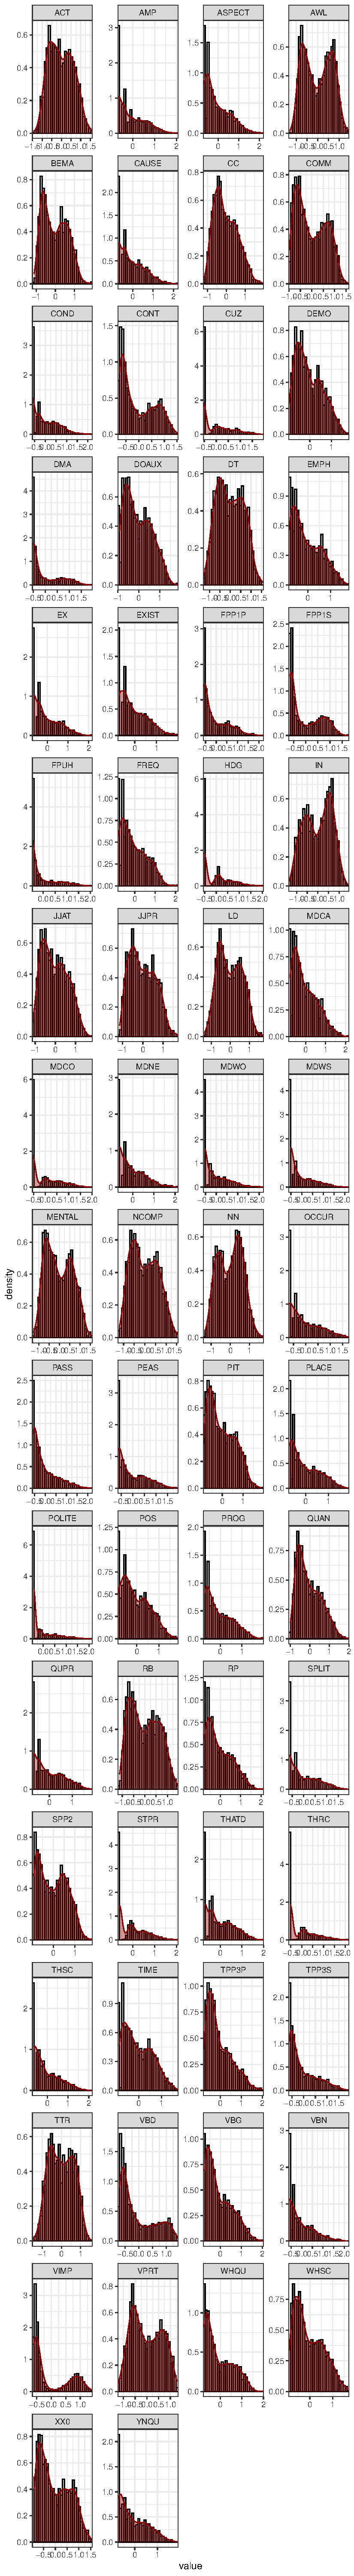
\includegraphics{D_Ch6_DataPrep_files/figure-pdf/signed.log.transformation-distributions-1.pdf}

\begin{Shaded}
\begin{Highlighting}[]
\CommentTok{\#ggsave(here("plots", "DensityPlotsAllVariablesSignedLog{-}TEC{-}only.svg"), width = 15, height = 49)}
\end{Highlighting}
\end{Shaded}

The following correlation plots serve to illustrate the effect of the
variable transformations performed in the above chunks.

Example feature distributions before transformations:

\begin{Shaded}
\begin{Highlighting}[]
\CommentTok{\# This is a slightly amended version of the PerformanceAnalytics::chart.Correlation() function. It simply removes the significance stars that are meaningless with this many data points (see commented out lines below)}

\NormalTok{chart.Correlation.nostars }\OtherTok{\textless{}{-}} \ControlFlowTok{function}\NormalTok{ (R, }\AttributeTok{histogram =} \ConstantTok{TRUE}\NormalTok{, }\AttributeTok{method =} \FunctionTok{c}\NormalTok{(}\StringTok{"pearson"}\NormalTok{, }\StringTok{"kendall"}\NormalTok{, }\StringTok{"spearman"}\NormalTok{), ...) \{}
\NormalTok{  x }\OtherTok{=} \FunctionTok{checkData}\NormalTok{(R, }\AttributeTok{method =} \StringTok{"matrix"}\NormalTok{)}
  \ControlFlowTok{if}\NormalTok{ (}\FunctionTok{missing}\NormalTok{(method)) }
\NormalTok{    method }\OtherTok{=}\NormalTok{ method[}\DecValTok{1}\NormalTok{]}
\NormalTok{  panel.cor }\OtherTok{\textless{}{-}} \ControlFlowTok{function}\NormalTok{(x, y, }\AttributeTok{digits =} \DecValTok{2}\NormalTok{, }\AttributeTok{prefix =} \StringTok{""}\NormalTok{, }\AttributeTok{use =} \StringTok{"pairwise.complete.obs"}\NormalTok{, }\AttributeTok{method =} \StringTok{"pearson"}\NormalTok{, cex.cor, ...) \{}
\NormalTok{    usr }\OtherTok{\textless{}{-}} \FunctionTok{par}\NormalTok{(}\StringTok{"usr"}\NormalTok{)}
    \FunctionTok{on.exit}\NormalTok{(}\FunctionTok{par}\NormalTok{(usr))}
    \FunctionTok{par}\NormalTok{(}\AttributeTok{usr =} \FunctionTok{c}\NormalTok{(}\DecValTok{0}\NormalTok{, }\DecValTok{1}\NormalTok{, }\DecValTok{0}\NormalTok{, }\DecValTok{1}\NormalTok{))}
\NormalTok{    r }\OtherTok{\textless{}{-}} \FunctionTok{cor}\NormalTok{(x, y, }\AttributeTok{use =}\NormalTok{ use, }\AttributeTok{method =}\NormalTok{ method)}
\NormalTok{    txt }\OtherTok{\textless{}{-}} \FunctionTok{format}\NormalTok{(}\FunctionTok{c}\NormalTok{(r, }\FloatTok{0.123456789}\NormalTok{), }\AttributeTok{digits =}\NormalTok{ digits)[}\DecValTok{1}\NormalTok{]}
\NormalTok{    txt }\OtherTok{\textless{}{-}} \FunctionTok{paste}\NormalTok{(prefix, txt, }\AttributeTok{sep =} \StringTok{""}\NormalTok{)}
    \ControlFlowTok{if}\NormalTok{ (}\FunctionTok{missing}\NormalTok{(cex.cor)) }
\NormalTok{      cex }\OtherTok{\textless{}{-}} \FloatTok{0.8}\SpecialCharTok{/}\FunctionTok{strwidth}\NormalTok{(txt)}
\NormalTok{    test }\OtherTok{\textless{}{-}} \FunctionTok{cor.test}\NormalTok{(}\FunctionTok{as.numeric}\NormalTok{(x), }\FunctionTok{as.numeric}\NormalTok{(y), }\AttributeTok{method =}\NormalTok{ method)}
    \CommentTok{\# Signif \textless{}{-} symnum(test$p.value, corr = FALSE, na = FALSE, }
    \CommentTok{\#                  cutpoints = c(0, 0.001, 0.01, 0.05, 0.1, 1), symbols = c("***", }
    \CommentTok{\#                                                                           "**", "*", ".", " "))}
    \FunctionTok{text}\NormalTok{(}\FloatTok{0.5}\NormalTok{, }\FloatTok{0.5}\NormalTok{, txt, }\AttributeTok{cex =}\NormalTok{ cex }\SpecialCharTok{*}\NormalTok{ (}\FunctionTok{abs}\NormalTok{(r) }\SpecialCharTok{+} \FloatTok{0.3}\NormalTok{)}\SpecialCharTok{/}\FloatTok{1.3}\NormalTok{)}
    \CommentTok{\# text(0.8, 0.8, Signif, cex = cex, col = 2)}
\NormalTok{  \}}
\NormalTok{  f }\OtherTok{\textless{}{-}} \ControlFlowTok{function}\NormalTok{(t) \{}
    \FunctionTok{dnorm}\NormalTok{(t, }\AttributeTok{mean =} \FunctionTok{mean}\NormalTok{(x), }\AttributeTok{sd =} \FunctionTok{sd.xts}\NormalTok{(x))}
\NormalTok{  \}}
\NormalTok{  dotargs }\OtherTok{\textless{}{-}} \FunctionTok{list}\NormalTok{(...)}
\NormalTok{  dotargs}\SpecialCharTok{$}\NormalTok{method }\OtherTok{\textless{}{-}} \ConstantTok{NULL}
  \FunctionTok{rm}\NormalTok{(method)}
\NormalTok{  hist.panel }\OtherTok{=} \ControlFlowTok{function}\NormalTok{(x, }\AttributeTok{... =} \ConstantTok{NULL}\NormalTok{) \{}
    \FunctionTok{par}\NormalTok{(}\AttributeTok{new =} \ConstantTok{TRUE}\NormalTok{)}
    \FunctionTok{hist}\NormalTok{(x, }\AttributeTok{col =} \StringTok{"light gray"}\NormalTok{, }\AttributeTok{probability =} \ConstantTok{TRUE}\NormalTok{, }
         \AttributeTok{axes =} \ConstantTok{FALSE}\NormalTok{, }\AttributeTok{main =} \StringTok{""}\NormalTok{, }\AttributeTok{breaks =} \StringTok{"FD"}\NormalTok{)}
    \FunctionTok{lines}\NormalTok{(}\FunctionTok{density}\NormalTok{(x, }\AttributeTok{na.rm =} \ConstantTok{TRUE}\NormalTok{), }\AttributeTok{col =} \StringTok{"red"}\NormalTok{, }\AttributeTok{lwd =} \DecValTok{1}\NormalTok{)}
    \FunctionTok{rug}\NormalTok{(x)}
\NormalTok{  \}}
  \ControlFlowTok{if}\NormalTok{ (histogram) }
    \FunctionTok{pairs}\NormalTok{(x, }\AttributeTok{gap =} \DecValTok{0}\NormalTok{, }\AttributeTok{lower.panel =}\NormalTok{ panel.smooth, }\AttributeTok{upper.panel =}\NormalTok{ panel.cor, }
          \AttributeTok{diag.panel =}\NormalTok{ hist.panel)}
  \ControlFlowTok{else} \FunctionTok{pairs}\NormalTok{(x, }\AttributeTok{gap =} \DecValTok{0}\NormalTok{, }\AttributeTok{lower.panel =}\NormalTok{ panel.smooth, }\AttributeTok{upper.panel =}\NormalTok{ panel.cor)}
\NormalTok{\}}

\CommentTok{\# Example plot without any variable transformation}
\NormalTok{example1 }\OtherTok{\textless{}{-}}\NormalTok{ TxBcounts }\SpecialCharTok{|\textgreater{}} 
  \FunctionTok{select}\NormalTok{(NN,PROG,SPLIT,ACT,FPP1S)}

\CommentTok{\#png(here("plots", "CorrChart{-}TEC{-}examples{-}normedcounts.png"), width = 20, height = 20, units = "cm", res = 300)}
\FunctionTok{chart.Correlation.nostars}\NormalTok{(example1, }\AttributeTok{histogram=}\ConstantTok{TRUE}\NormalTok{, }\AttributeTok{pch=}\DecValTok{19}\NormalTok{)}
\end{Highlighting}
\end{Shaded}

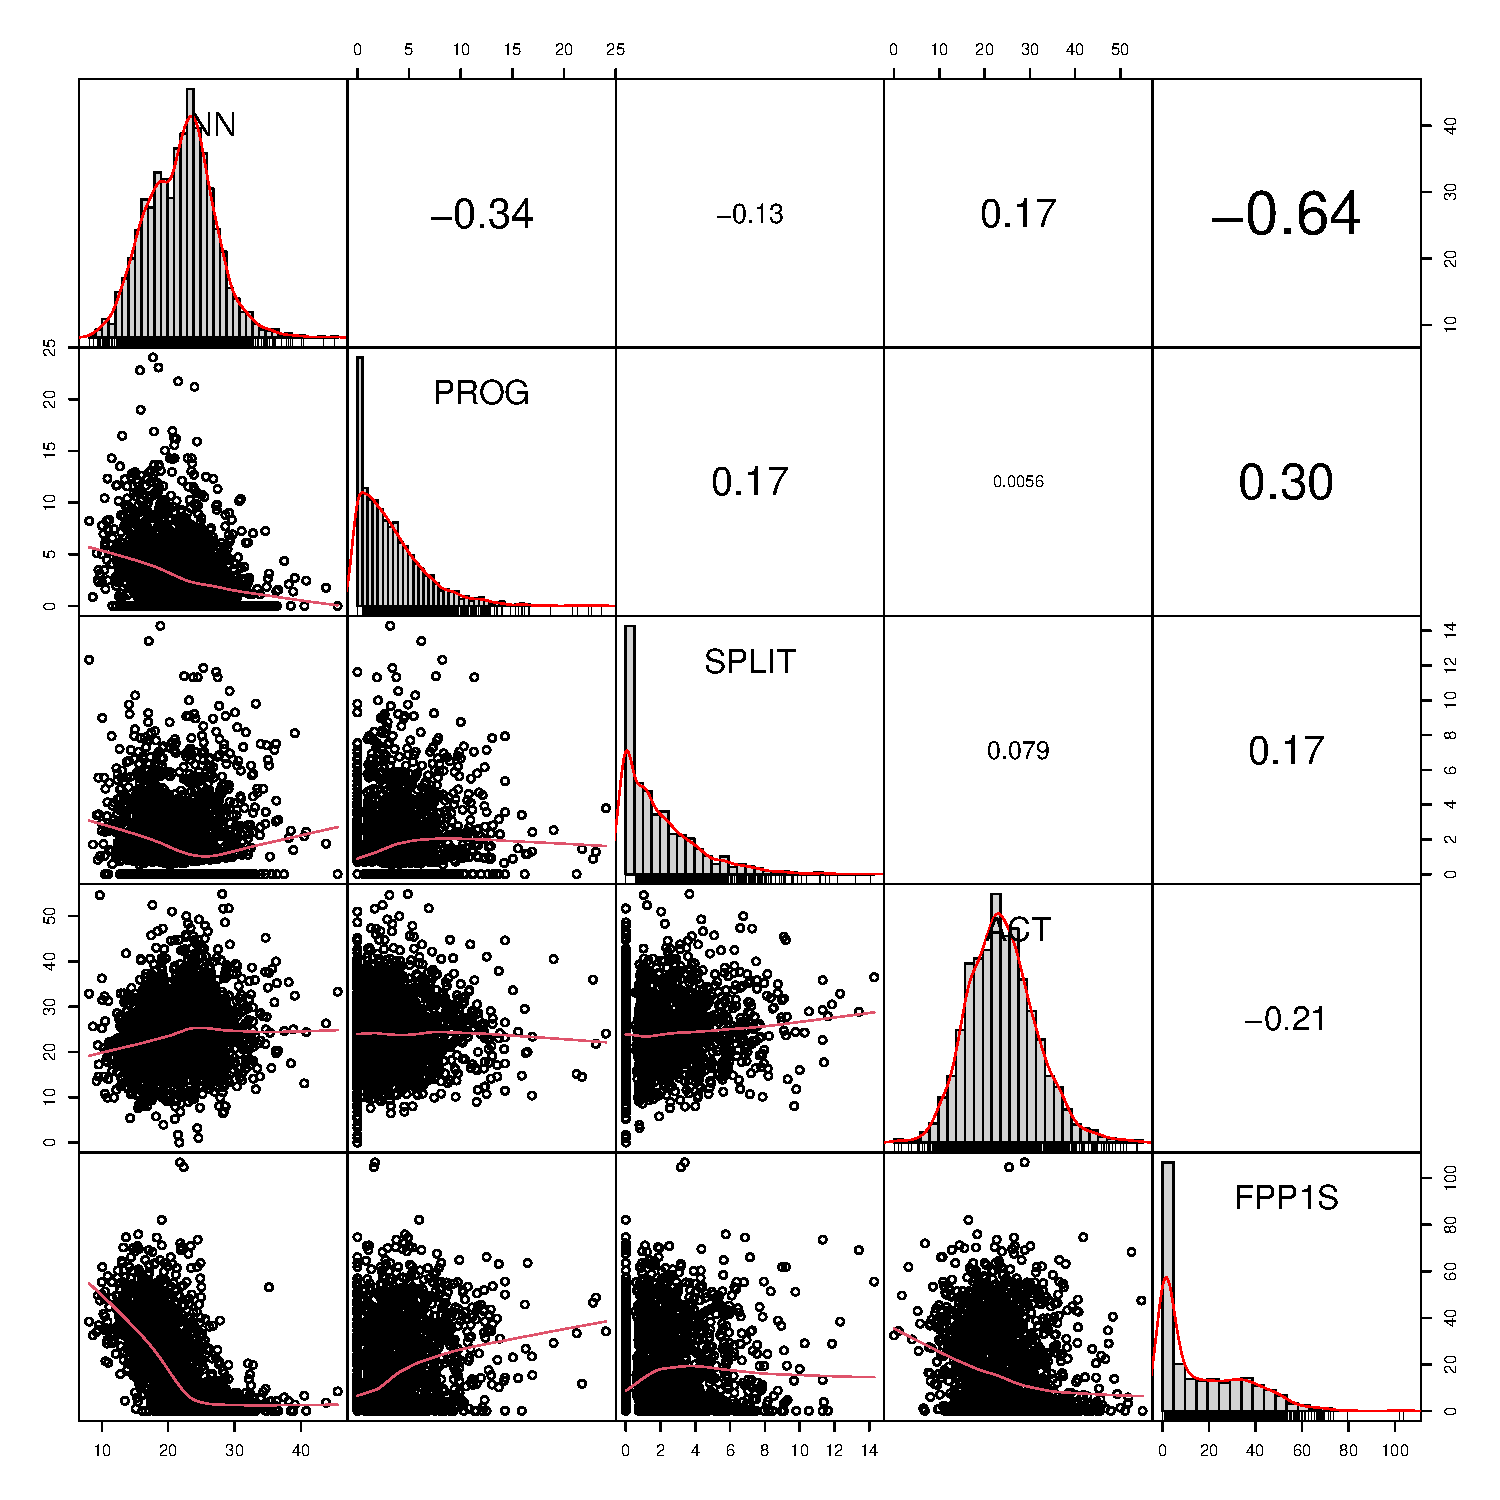
\includegraphics{D_Ch6_DataPrep_files/figure-pdf/example-correlation-plots-1.pdf}

\begin{Shaded}
\begin{Highlighting}[]
\CommentTok{\#dev.off()}
\end{Highlighting}
\end{Shaded}

Example feature distributions after transformations:

\begin{Shaded}
\begin{Highlighting}[]
\CommentTok{\# Example plot with transformed variables}
\NormalTok{example2 }\OtherTok{\textless{}{-}}\NormalTok{ TxBzlogcounts }\SpecialCharTok{|\textgreater{}} 
  \FunctionTok{as.data.frame}\NormalTok{() }\SpecialCharTok{|\textgreater{}}  
  \FunctionTok{select}\NormalTok{(NN,PROG,SPLIT,ACT,FPP1S)}

\CommentTok{\#png(here("plots", "CorrChart{-}TEC{-}examples{-}zsignedlogcounts.png"), width = 20, height = 20, units = "cm", res = 300)}
\FunctionTok{chart.Correlation.nostars}\NormalTok{(example2, }\AttributeTok{histogram=}\ConstantTok{TRUE}\NormalTok{, }\AttributeTok{pch=}\DecValTok{19}\NormalTok{)}
\end{Highlighting}
\end{Shaded}

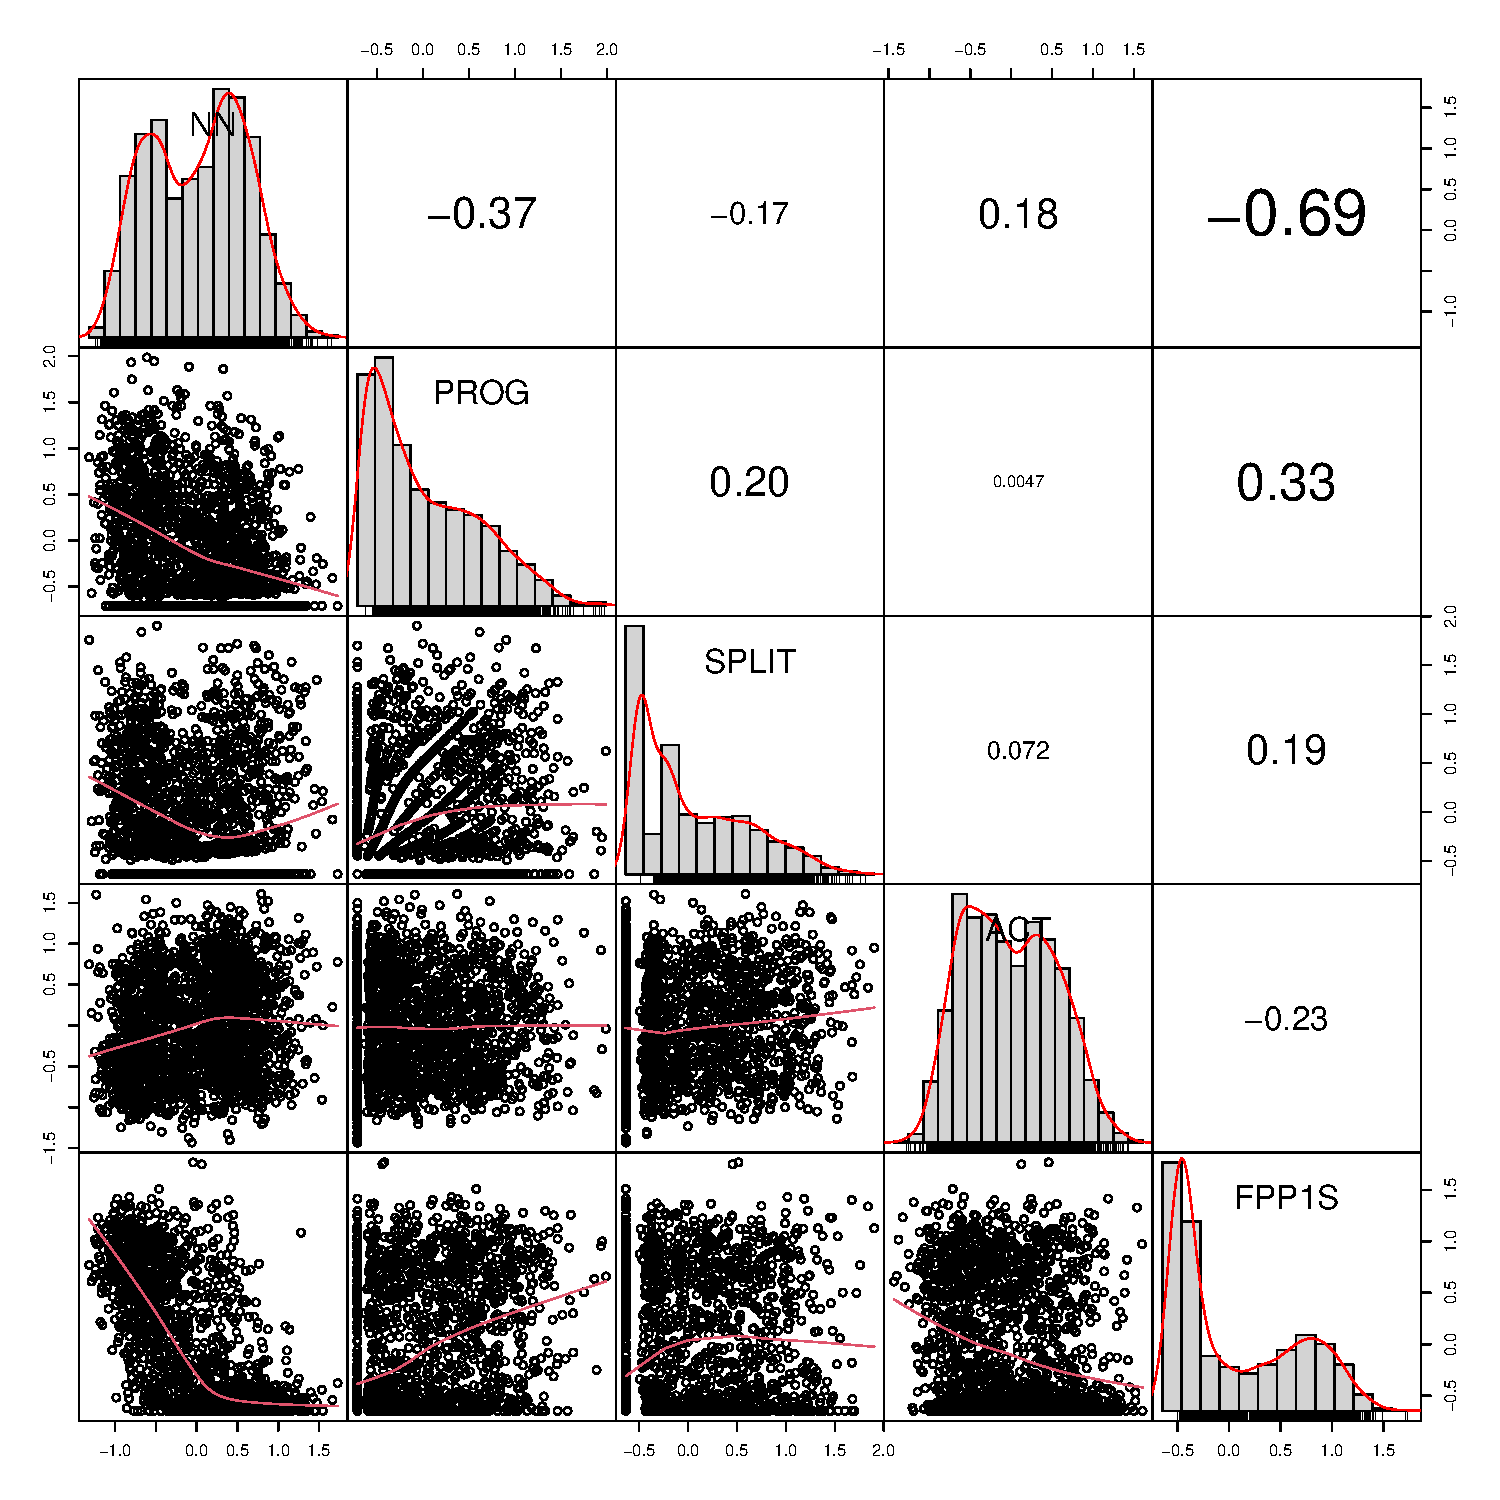
\includegraphics{D_Ch6_DataPrep_files/figure-pdf/example-correlation-plots2-1.pdf}

\begin{Shaded}
\begin{Highlighting}[]
\CommentTok{\#dev.off()}
\end{Highlighting}
\end{Shaded}

\subsection{Feature correlations}\label{feature-correlations}

The correlations of the transformed feature frequencies can be
visualised in the form of a heatmap. Negative correlations are rendered
in blue, whereas positive ones are in red.

\begin{Shaded}
\begin{Highlighting}[]
\CommentTok{\# Simple heatmap in base R (inspired by Stephanie Evert\textquotesingle{}s SIGIL code)}
\NormalTok{cor.colours }\OtherTok{\textless{}{-}} \FunctionTok{c}\NormalTok{(}
  \FunctionTok{hsv}\NormalTok{(}\AttributeTok{h=}\DecValTok{2}\SpecialCharTok{/}\DecValTok{3}\NormalTok{, }\AttributeTok{v=}\DecValTok{1}\NormalTok{, }\AttributeTok{s=}\NormalTok{(}\DecValTok{10}\SpecialCharTok{:}\DecValTok{1}\NormalTok{)}\SpecialCharTok{/}\DecValTok{10}\NormalTok{), }\CommentTok{\# blue = negative correlation }
  \FunctionTok{rgb}\NormalTok{(}\DecValTok{1}\NormalTok{,}\DecValTok{1}\NormalTok{,}\DecValTok{1}\NormalTok{), }\CommentTok{\# white = no correlation }
  \FunctionTok{hsv}\NormalTok{(}\AttributeTok{h=}\DecValTok{0}\NormalTok{, }\AttributeTok{v=}\DecValTok{1}\NormalTok{, }\AttributeTok{s=}\NormalTok{(}\DecValTok{1}\SpecialCharTok{:}\DecValTok{10}\SpecialCharTok{/}\DecValTok{10}\NormalTok{))) }\CommentTok{\# red = positive correlation}

\CommentTok{\#png(here("plots", "heatmapzlogcounts{-}TEC{-}only.png"), width = 30, height= 30, units = "cm", res = 300)}
\FunctionTok{heatmap}\NormalTok{(}\FunctionTok{cor}\NormalTok{(TxBzlogcounts), }
        \AttributeTok{symm=}\ConstantTok{TRUE}\NormalTok{, }
        \AttributeTok{zlim=}\FunctionTok{c}\NormalTok{(}\SpecialCharTok{{-}}\DecValTok{1}\NormalTok{,}\DecValTok{1}\NormalTok{), }
        \AttributeTok{col=}\NormalTok{cor.colours, }
        \AttributeTok{margins=}\FunctionTok{c}\NormalTok{(}\DecValTok{0}\NormalTok{,}\DecValTok{0}\NormalTok{))}
\end{Highlighting}
\end{Shaded}

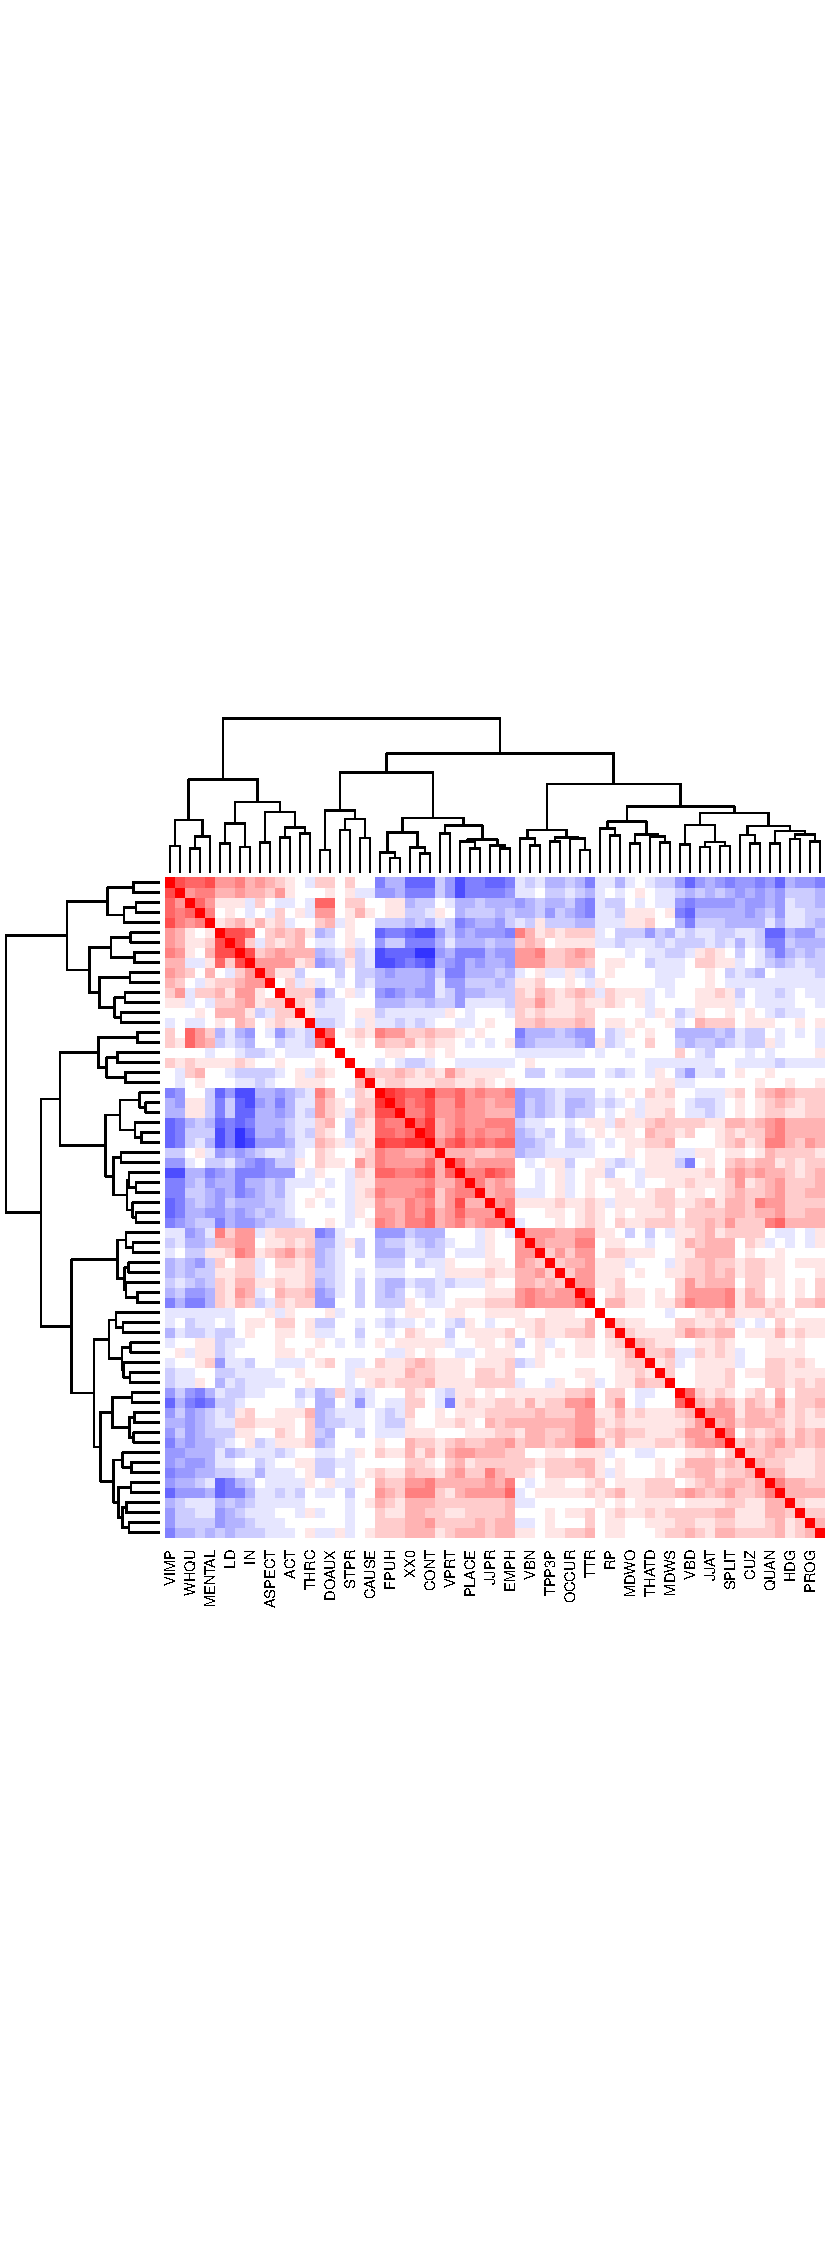
\includegraphics{D_Ch6_DataPrep_files/figure-pdf/heatmap-1.pdf}

\begin{Shaded}
\begin{Highlighting}[]
\CommentTok{\#dev.off()}

\CommentTok{\# Calculate the sum of all the words in the tagged texts of the TEC}
\NormalTok{totalwords }\OtherTok{\textless{}{-}}\NormalTok{ TxBcounts }\SpecialCharTok{|\textgreater{}}  
  \FunctionTok{select}\NormalTok{(Words) }\SpecialCharTok{|\textgreater{}} 
  \FunctionTok{sum}\NormalTok{() }\SpecialCharTok{|\textgreater{}} 
  \FunctionTok{format}\NormalTok{(}\AttributeTok{big.mark=}\StringTok{","}\NormalTok{)}
\end{Highlighting}
\end{Shaded}

\section{Composition of TEC
texts/files}\label{composition-of-tec-textsfiles}

These figures and tables provide summary statistics on the texts/files
of the TEC that were entered in the multi-dimensional model of
intra-textbook linguistic variation. In total, the TEC texts entered
amounted to 1,693,650 words.

\begin{Shaded}
\begin{Highlighting}[]
\NormalTok{metadata }\OtherTok{\textless{}{-}}\NormalTok{ TxBcounts }\SpecialCharTok{|\textgreater{}}  
  \FunctionTok{select}\NormalTok{(Filename, Country, Series, Level, Register, Words) }\SpecialCharTok{|\textgreater{}}  
  \FunctionTok{mutate}\NormalTok{(}\AttributeTok{Volume =} \FunctionTok{paste}\NormalTok{(Series, Level)) }\SpecialCharTok{|\textgreater{}}  
  \FunctionTok{mutate}\NormalTok{(}\AttributeTok{Volume =} \FunctionTok{fct\_rev}\NormalTok{(Volume)) }\SpecialCharTok{|\textgreater{}}  
  \FunctionTok{mutate}\NormalTok{(}\AttributeTok{Volume =} \FunctionTok{fct\_reorder}\NormalTok{(Volume, }\FunctionTok{as.numeric}\NormalTok{(Level))) }\SpecialCharTok{|\textgreater{}}  
  \FunctionTok{group\_by}\NormalTok{(Volume) }\SpecialCharTok{|\textgreater{}}  
  \FunctionTok{mutate}\NormalTok{(}\AttributeTok{wordcount =} \FunctionTok{sum}\NormalTok{(Words)) }\SpecialCharTok{|\textgreater{}}  
  \FunctionTok{ungroup}\NormalTok{() }\SpecialCharTok{|\textgreater{}}  
  \FunctionTok{distinct}\NormalTok{(Volume, }\AttributeTok{.keep\_all =} \ConstantTok{TRUE}\NormalTok{)}

\CommentTok{\# Plot for book}
\NormalTok{metadata2 }\OtherTok{\textless{}{-}}\NormalTok{ TxBcounts }\SpecialCharTok{|\textgreater{}}  
  \FunctionTok{select}\NormalTok{(Country, Series, Level, Register, Words) }\SpecialCharTok{|\textgreater{}}  
  \FunctionTok{mutate}\NormalTok{(}\AttributeTok{Volume =} \FunctionTok{paste}\NormalTok{(Series, Level)) }\SpecialCharTok{|\textgreater{}}  
  \FunctionTok{mutate}\NormalTok{(}\AttributeTok{Volume =} \FunctionTok{fct\_rev}\NormalTok{(Volume)) }\SpecialCharTok{|\textgreater{}}  
  \CommentTok{\#mutate(Volume = fct\_reorder(Volume, as.numeric(Level))) |\textgreater{}  }
  \FunctionTok{group\_by}\NormalTok{(Volume, Register) }\SpecialCharTok{|\textgreater{}}  
  \FunctionTok{mutate}\NormalTok{(}\AttributeTok{wordcount =} \FunctionTok{sum}\NormalTok{(Words)) }\SpecialCharTok{|\textgreater{}}  
  \FunctionTok{ungroup}\NormalTok{() }\SpecialCharTok{|\textgreater{}}  
  \FunctionTok{distinct}\NormalTok{(Volume, Register, }\AttributeTok{.keep\_all =} \ConstantTok{TRUE}\NormalTok{)}

\CommentTok{\# This is the palette created above on the basis of the suffrager pakcage (but without needed to install the package)}
\NormalTok{palette }\OtherTok{\textless{}{-}} \FunctionTok{c}\NormalTok{(}\StringTok{"\#BD241E"}\NormalTok{, }\StringTok{"\#A18A33"}\NormalTok{, }\StringTok{"\#15274D"}\NormalTok{, }\StringTok{"\#D54E1E"}\NormalTok{, }\StringTok{"\#EA7E1E"}\NormalTok{, }\StringTok{"\#4C4C4C"}\NormalTok{, }\StringTok{"\#722672"}\NormalTok{, }\StringTok{"\#F9B921"}\NormalTok{, }\StringTok{"\#267226"}\NormalTok{)}

\NormalTok{PlotSp }\OtherTok{\textless{}{-}}\NormalTok{ metadata2 }\SpecialCharTok{|\textgreater{}}  
  \FunctionTok{filter}\NormalTok{(Country}\SpecialCharTok{==}\StringTok{"Spain"}\NormalTok{) }\SpecialCharTok{|\textgreater{}}  
  \CommentTok{\#arrange(Volume) |\textgreater{}  }
  \FunctionTok{ggplot}\NormalTok{(}\FunctionTok{aes}\NormalTok{(}\AttributeTok{x =}\NormalTok{ Volume, }\AttributeTok{y =}\NormalTok{ wordcount, }\AttributeTok{fill =} \FunctionTok{fct\_rev}\NormalTok{(Register))) }\SpecialCharTok{+} 
    \FunctionTok{geom\_bar}\NormalTok{(}\AttributeTok{stat =} \StringTok{"identity"}\NormalTok{, }\AttributeTok{position =} \StringTok{"stack"}\NormalTok{) }\SpecialCharTok{+}
    \FunctionTok{coord\_flip}\NormalTok{(}\AttributeTok{expand =} \ConstantTok{FALSE}\NormalTok{) }\SpecialCharTok{+} \CommentTok{\# Removes those annoying ticks before each bar label}
    \FunctionTok{theme\_minimal}\NormalTok{() }\SpecialCharTok{+} \FunctionTok{theme}\NormalTok{(}\AttributeTok{legend.position =} \StringTok{"none"}\NormalTok{) }\SpecialCharTok{+}
    \FunctionTok{labs}\NormalTok{(}\AttributeTok{x =} \StringTok{"Spain"}\NormalTok{, }\AttributeTok{y =} \StringTok{"Cumulative word count"}\NormalTok{) }\SpecialCharTok{+}
    \FunctionTok{scale\_fill\_manual}\NormalTok{(}\AttributeTok{values =}\NormalTok{ palette[}\FunctionTok{c}\NormalTok{(}\DecValTok{5}\NormalTok{,}\DecValTok{4}\NormalTok{,}\DecValTok{3}\NormalTok{,}\DecValTok{2}\NormalTok{,}\DecValTok{1}\NormalTok{)], }
                      \AttributeTok{guide =} \FunctionTok{guide\_legend}\NormalTok{(}\AttributeTok{reverse =} \ConstantTok{TRUE}\NormalTok{))}

\NormalTok{PlotGer }\OtherTok{\textless{}{-}}\NormalTok{ metadata2 }\SpecialCharTok{|\textgreater{}}  
  \FunctionTok{filter}\NormalTok{(Country}\SpecialCharTok{==}\StringTok{"Germany"}\NormalTok{) }\SpecialCharTok{|\textgreater{}}  
  \CommentTok{\#arrange(Volume) |\textgreater{}  }
  \FunctionTok{ggplot}\NormalTok{(}\FunctionTok{aes}\NormalTok{(}\AttributeTok{x =}\NormalTok{ Volume, }\AttributeTok{y =}\NormalTok{ wordcount, }\AttributeTok{fill =} \FunctionTok{fct\_rev}\NormalTok{(Register))) }\SpecialCharTok{+} 
    \FunctionTok{geom\_bar}\NormalTok{(}\AttributeTok{stat =} \StringTok{"identity"}\NormalTok{, }\AttributeTok{position =} \StringTok{"stack"}\NormalTok{) }\SpecialCharTok{+}
    \FunctionTok{coord\_flip}\NormalTok{(}\AttributeTok{expand =} \ConstantTok{FALSE}\NormalTok{) }\SpecialCharTok{+}
    \FunctionTok{labs}\NormalTok{(}\AttributeTok{x =} \StringTok{"Germany"}\NormalTok{, }\AttributeTok{y =} \StringTok{""}\NormalTok{) }\SpecialCharTok{+}
    \FunctionTok{scale\_fill\_manual}\NormalTok{(}\AttributeTok{values =}\NormalTok{ palette[}\FunctionTok{c}\NormalTok{(}\DecValTok{5}\NormalTok{,}\DecValTok{4}\NormalTok{,}\DecValTok{3}\NormalTok{,}\DecValTok{2}\NormalTok{,}\DecValTok{1}\NormalTok{)], }\AttributeTok{guide =} \FunctionTok{guide\_legend}\NormalTok{(}\AttributeTok{reverse =} \ConstantTok{TRUE}\NormalTok{)) }\SpecialCharTok{+}
    \FunctionTok{theme\_minimal}\NormalTok{() }\SpecialCharTok{+} \FunctionTok{theme}\NormalTok{(}\AttributeTok{legend.position =} \StringTok{"none"}\NormalTok{)}

\NormalTok{PlotFr }\OtherTok{\textless{}{-}}\NormalTok{ metadata2 }\SpecialCharTok{|\textgreater{}}  
  \FunctionTok{filter}\NormalTok{(Country}\SpecialCharTok{==}\StringTok{"France"}\NormalTok{) }\SpecialCharTok{|\textgreater{}}  
  \CommentTok{\#arrange(Volume) |\textgreater{}  }
  \FunctionTok{ggplot}\NormalTok{(}\FunctionTok{aes}\NormalTok{(}\AttributeTok{x =}\NormalTok{ Volume, }\AttributeTok{y =}\NormalTok{ wordcount, }\AttributeTok{fill =} \FunctionTok{fct\_rev}\NormalTok{(Register))) }\SpecialCharTok{+} 
    \FunctionTok{geom\_bar}\NormalTok{(}\AttributeTok{stat =} \StringTok{"identity"}\NormalTok{, }\AttributeTok{position =} \StringTok{"stack"}\NormalTok{) }\SpecialCharTok{+}
    \FunctionTok{coord\_flip}\NormalTok{(}\AttributeTok{expand =} \ConstantTok{FALSE}\NormalTok{) }\SpecialCharTok{+}
    \FunctionTok{labs}\NormalTok{(}\AttributeTok{x =} \StringTok{"France"}\NormalTok{, }\AttributeTok{y  =} \StringTok{""}\NormalTok{, }\AttributeTok{fill =} \StringTok{"Register subcorpus"}\NormalTok{) }\SpecialCharTok{+}
    \FunctionTok{scale\_fill\_manual}\NormalTok{(}\AttributeTok{values =}\NormalTok{ palette[}\FunctionTok{c}\NormalTok{(}\DecValTok{5}\NormalTok{,}\DecValTok{4}\NormalTok{,}\DecValTok{3}\NormalTok{,}\DecValTok{2}\NormalTok{,}\DecValTok{1}\NormalTok{)], }\AttributeTok{guide =} \FunctionTok{guide\_legend}\NormalTok{(}\AttributeTok{reverse =} \ConstantTok{TRUE}\NormalTok{, }\AttributeTok{legend.hjust =} \DecValTok{0}\NormalTok{)) }\SpecialCharTok{+}
    \FunctionTok{theme\_minimal}\NormalTok{() }\SpecialCharTok{+} \FunctionTok{theme}\NormalTok{(}\AttributeTok{legend.position =} \StringTok{"top"}\NormalTok{, }\AttributeTok{legend.justification =} \StringTok{"left"}\NormalTok{)}

\NormalTok{PlotFr }\SpecialCharTok{/}
\NormalTok{PlotGer }\SpecialCharTok{/}
\NormalTok{PlotSp}
\end{Highlighting}
\end{Shaded}

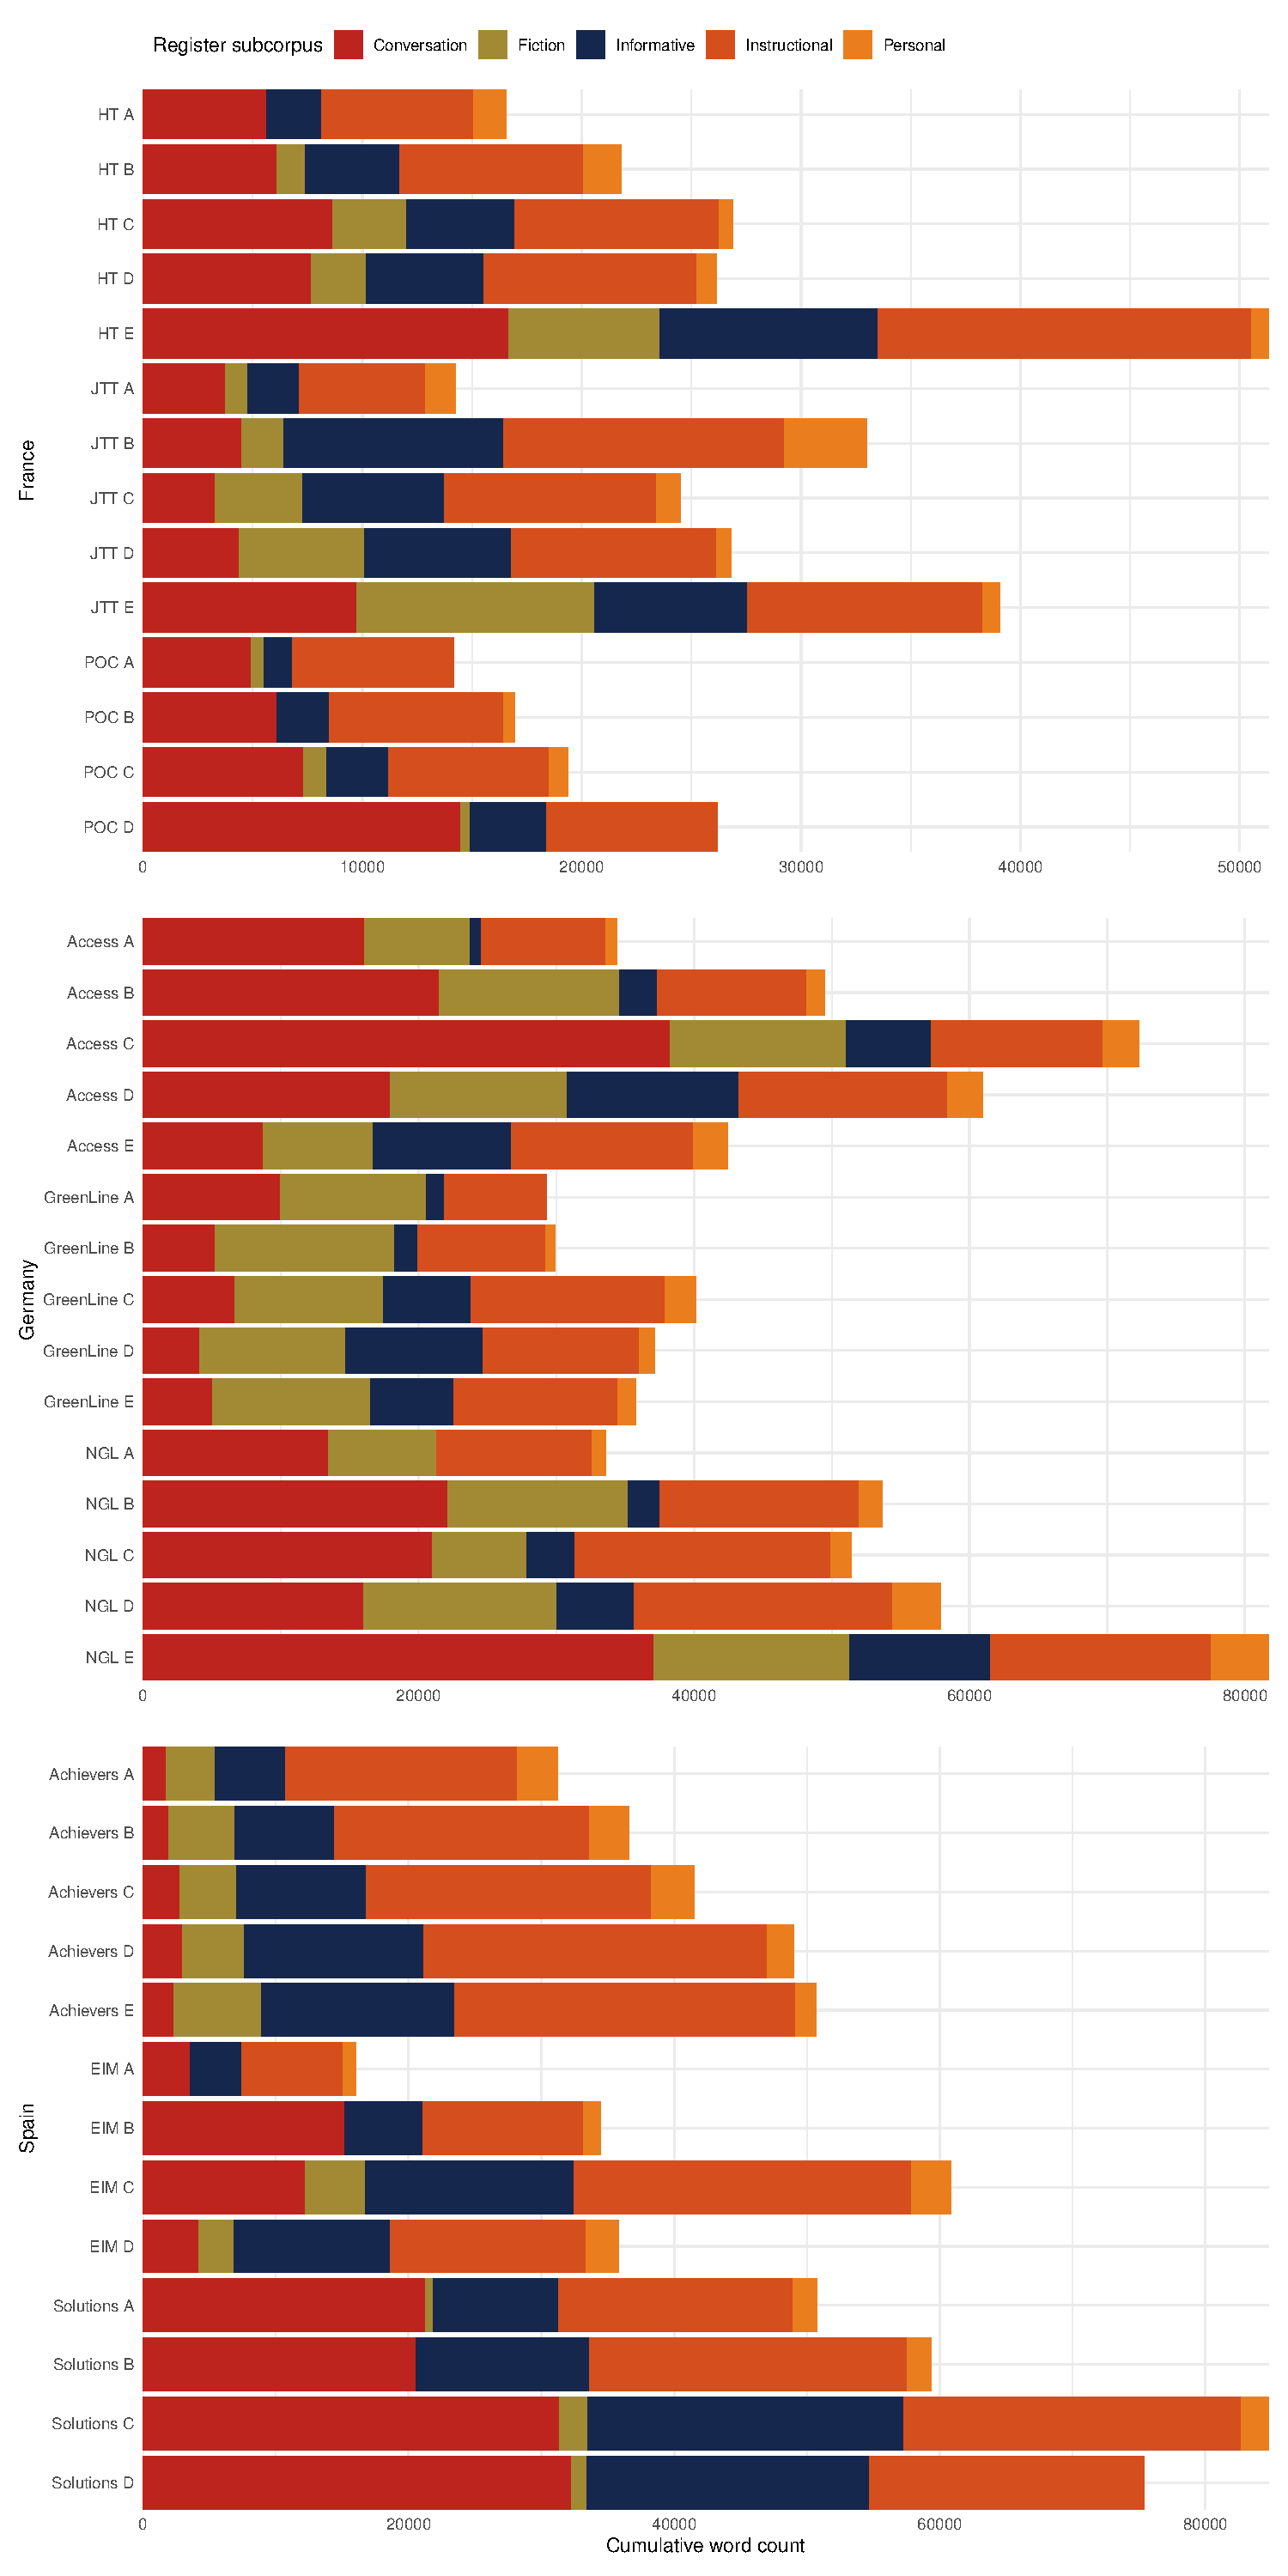
\includegraphics{D_Ch6_DataPrep_files/figure-pdf/TEC-metadata-1.pdf}

\begin{Shaded}
\begin{Highlighting}[]
\CommentTok{\#ggsave(here("plots", "TEC{-}T\_wordcounts\_book.svg"), width = 8, height = 12)}
\end{Highlighting}
\end{Shaded}

The following table provides information about the proportion of
instructional language featured in each textbook series.

\begin{Shaded}
\begin{Highlighting}[]
\NormalTok{metadataInstr }\OtherTok{\textless{}{-}}\NormalTok{ TxBcounts }\SpecialCharTok{|\textgreater{}}  
  \FunctionTok{select}\NormalTok{(Country, Series, Level, Register, Words) }\SpecialCharTok{|\textgreater{}}  
  \FunctionTok{filter}\NormalTok{(Register}\SpecialCharTok{==}\StringTok{"Instructional"}\NormalTok{) }\SpecialCharTok{|\textgreater{}}  
  \FunctionTok{mutate}\NormalTok{(}\AttributeTok{Volume =} \FunctionTok{paste}\NormalTok{(Series, Register)) }\SpecialCharTok{|\textgreater{}}  
  \FunctionTok{mutate}\NormalTok{(}\AttributeTok{Volume =} \FunctionTok{fct\_rev}\NormalTok{(Volume)) }\SpecialCharTok{|\textgreater{}}  
  \FunctionTok{mutate}\NormalTok{(}\AttributeTok{Volume =} \FunctionTok{fct\_reorder}\NormalTok{(Volume, }\FunctionTok{as.numeric}\NormalTok{(Level))) }\SpecialCharTok{|\textgreater{}}  
  \FunctionTok{group\_by}\NormalTok{(Volume, Register) }\SpecialCharTok{|\textgreater{}}  
  \FunctionTok{mutate}\NormalTok{(}\AttributeTok{InstrWordcount =} \FunctionTok{sum}\NormalTok{(Words)) }\SpecialCharTok{|\textgreater{}}  
  \FunctionTok{ungroup}\NormalTok{() }\SpecialCharTok{|\textgreater{}}  
  \FunctionTok{distinct}\NormalTok{(Volume, }\AttributeTok{.keep\_all =} \ConstantTok{TRUE}\NormalTok{) }\SpecialCharTok{|\textgreater{}}  
  \FunctionTok{select}\NormalTok{(Series, InstrWordcount)}

\NormalTok{metaWordcount }\OtherTok{\textless{}{-}}\NormalTok{ TxBcounts }\SpecialCharTok{|\textgreater{}}  
  \FunctionTok{select}\NormalTok{(Country, Series, Level, Register, Words) }\SpecialCharTok{|\textgreater{}}  
  \FunctionTok{group\_by}\NormalTok{(Series) }\SpecialCharTok{|\textgreater{}}  
  \FunctionTok{mutate}\NormalTok{(}\AttributeTok{TECwordcount =} \FunctionTok{sum}\NormalTok{(Words)) }\SpecialCharTok{|\textgreater{}}  
  \FunctionTok{ungroup}\NormalTok{() }\SpecialCharTok{|\textgreater{}}  
  \FunctionTok{distinct}\NormalTok{(Series, }\AttributeTok{.keep\_all =} \ConstantTok{TRUE}\NormalTok{) }\SpecialCharTok{|\textgreater{}}  
  \FunctionTok{select}\NormalTok{(Series, TECwordcount)}

\NormalTok{wordcount }\OtherTok{\textless{}{-}} \FunctionTok{merge}\NormalTok{(metaWordcount, metadataInstr, }\AttributeTok{by =} \StringTok{"Series"}\NormalTok{)}

\NormalTok{wordcount }\SpecialCharTok{|\textgreater{}}  
  \FunctionTok{mutate}\NormalTok{(}\AttributeTok{InstrucPercent =}\NormalTok{ InstrWordcount}\SpecialCharTok{/}\NormalTok{TECwordcount}\SpecialCharTok{*}\DecValTok{100}\NormalTok{) }\SpecialCharTok{|\textgreater{}}  
  \FunctionTok{arrange}\NormalTok{(InstrucPercent) }\SpecialCharTok{|\textgreater{}}  
  \FunctionTok{mutate}\NormalTok{(}\AttributeTok{InstrucPercent =} \FunctionTok{round}\NormalTok{(InstrucPercent, }\DecValTok{2}\NormalTok{)) }\SpecialCharTok{|\textgreater{}}  
  \FunctionTok{kable}\NormalTok{(}\AttributeTok{col.names =} \FunctionTok{c}\NormalTok{(}\StringTok{"Textbook Series"}\NormalTok{, }\StringTok{"Total words"}\NormalTok{, }\StringTok{"Instructional words"}\NormalTok{, }\StringTok{"\% of textbook content"}\NormalTok{), }
        \AttributeTok{digits =} \DecValTok{2}\NormalTok{, }
        \AttributeTok{format.args =} \FunctionTok{list}\NormalTok{(}\AttributeTok{big.mark =} \StringTok{","}\NormalTok{))}
\end{Highlighting}
\end{Shaded}

\begin{longtable}[]{@{}
  >{\raggedright\arraybackslash}p{(\columnwidth - 6\tabcolsep) * \real{0.2286}}
  >{\raggedleft\arraybackslash}p{(\columnwidth - 6\tabcolsep) * \real{0.1714}}
  >{\raggedleft\arraybackslash}p{(\columnwidth - 6\tabcolsep) * \real{0.2857}}
  >{\raggedleft\arraybackslash}p{(\columnwidth - 6\tabcolsep) * \real{0.3143}}@{}}
\toprule\noalign{}
\begin{minipage}[b]{\linewidth}\raggedright
Textbook Series
\end{minipage} & \begin{minipage}[b]{\linewidth}\raggedleft
Total words
\end{minipage} & \begin{minipage}[b]{\linewidth}\raggedleft
Instructional words
\end{minipage} & \begin{minipage}[b]{\linewidth}\raggedleft
\% of textbook content
\end{minipage} \\
\midrule\noalign{}
\endhead
\bottomrule\noalign{}
\endlastfoot
Access & 259,679 & 60,938 & 23.47 \\
NGL & 278,316 & 79,312 & 28.50 \\
GreenLine & 172,267 & 54,263 & 31.50 \\
Solutions & 270,278 & 87,829 & 32.50 \\
JTT & 137,557 & 48,375 & 35.17 \\
HT & 142,676 & 51,550 & 36.13 \\
POC & 76,714 & 30,548 & 39.82 \\
EIM & 147,185 & 59,928 & 40.72 \\
Achievers & 208,978 & 109,886 & 52.58 \\
\end{longtable}

\chapter{Data Analysis for the Model of Intra-Textbook
Variation}\label{data-analysis-for-the-model-of-intra-textbook-variation}

This script documents the analysis of the pre-processed data from the
Textbook English Corpus (TEC) to arrive at the multi-dimensional model
of intra-textbook linguistic variation (Chapter 6). It generates all of
the statistics and plots included in the book, as well as many others
that were used in the analysis, but not included in the book for reasons
of space.

\section{Packages required}\label{packages-required-1}

The following packages must be installed and loaded to carry out the
following analyses.

\begin{Shaded}
\begin{Highlighting}[]
\CommentTok{\#renv::restore() \# Restore the project\textquotesingle{}s dependencies from the lockfile to ensure that same package versions are used as in the original study}

\FunctionTok{library}\NormalTok{(caret) }\CommentTok{\# For its confusion matrix function}
\FunctionTok{library}\NormalTok{(cowplot)}
\FunctionTok{library}\NormalTok{(DescTools) }\CommentTok{\# For 95\% CI}
\FunctionTok{library}\NormalTok{(emmeans)}
\FunctionTok{library}\NormalTok{(factoextra) }\CommentTok{\# For circular graphs of variables}
\FunctionTok{library}\NormalTok{(forcats) }\CommentTok{\# For data manipulation}
\FunctionTok{library}\NormalTok{(ggthemes) }\CommentTok{\# For theme of factoextra plots}
\FunctionTok{library}\NormalTok{(here) }\CommentTok{\# For dynamic file paths}
\FunctionTok{library}\NormalTok{(knitr) }\CommentTok{\# Loaded to display the tables using the kable() function}
\FunctionTok{library}\NormalTok{(lme4) }\CommentTok{\# For linear regression modelling}
\FunctionTok{library}\NormalTok{(patchwork) }\CommentTok{\# To create figures with more than one plot}
\FunctionTok{library}\NormalTok{(PCAtools) }\CommentTok{\# For nice biplots of PCA results}
\FunctionTok{library}\NormalTok{(psych) }\CommentTok{\# For various useful stats function}
\FunctionTok{library}\NormalTok{(sjPlot) }\CommentTok{\# For model plots and tables}
\FunctionTok{library}\NormalTok{(tidyverse) }\CommentTok{\# For data wrangling}
\FunctionTok{library}\NormalTok{(visreg) }\CommentTok{\# For plots of interaction effects}

\CommentTok{\# From https://github.com/RainCloudPlots/RainCloudPlots:}
\FunctionTok{source}\NormalTok{(}\FunctionTok{here}\NormalTok{(}\StringTok{"R\_rainclouds.R"}\NormalTok{)) }\CommentTok{\# For geom\_flat\_violin rainplots}
\end{Highlighting}
\end{Shaded}

\section{Preparing the data for PCA}\label{preparing-the-data-for-pca}

\subsection{TEC data import}\label{tec-data-import}

\begin{Shaded}
\begin{Highlighting}[]
\NormalTok{TxBcounts }\OtherTok{\textless{}{-}} \FunctionTok{readRDS}\NormalTok{(}\FunctionTok{here}\NormalTok{(}\StringTok{"data"}\NormalTok{, }\StringTok{"processed"}\NormalTok{, }\StringTok{"TxBcounts3.rds"}\NormalTok{))}
\CommentTok{\# colnames(TxBcounts)}
\CommentTok{\# nrow(TxBcounts)}

\NormalTok{TxBzlogcounts }\OtherTok{\textless{}{-}} \FunctionTok{readRDS}\NormalTok{(}\FunctionTok{here}\NormalTok{(}\StringTok{"data"}\NormalTok{, }\StringTok{"processed"}\NormalTok{, }\StringTok{"TxBzlogcounts.rds"}\NormalTok{)) }
\CommentTok{\# nrow(TxBzlogcounts)}
\CommentTok{\# colnames(TxBzlogcounts)}

\NormalTok{TxBdata }\OtherTok{\textless{}{-}} \FunctionTok{cbind}\NormalTok{(TxBcounts[,}\DecValTok{1}\SpecialCharTok{:}\DecValTok{6}\NormalTok{], }\FunctionTok{as.data.frame}\NormalTok{(TxBzlogcounts))}
\CommentTok{\# str(TxBdata)}
\end{Highlighting}
\end{Shaded}

First, the TEC data as processed in Appendix D is imported. It comprises
1,961 texts/files, each with logged standardised normalised frequencies
for 66 linguistic features.

\section{Checking the factorability of
data}\label{checking-the-factorability-of-data}

\begin{Shaded}
\begin{Highlighting}[]
\NormalTok{kmo }\OtherTok{\textless{}{-}} \FunctionTok{KMO}\NormalTok{(TxBdata[,}\DecValTok{7}\SpecialCharTok{:}\FunctionTok{ncol}\NormalTok{(TxBdata)]) }
\end{Highlighting}
\end{Shaded}

The overall MSA value of the dataset is 0.86. The features have the
following individual MSA values (ordered from lowest to largest):

\begin{Shaded}
\begin{Highlighting}[]
\NormalTok{kmo}\SpecialCharTok{$}\NormalTok{MSAi[}\FunctionTok{order}\NormalTok{(kmo}\SpecialCharTok{$}\NormalTok{MSAi)] }\SpecialCharTok{|\textgreater{}}  \FunctionTok{round}\NormalTok{(}\DecValTok{2}\NormalTok{)}
\end{Highlighting}
\end{Shaded}

\begin{verbatim}
  MDWO   MDWS   MDNE   MDCA    VBD   VPRT    POS    ACT   FREQ  TPP3S     LD 
  0.34   0.46   0.52   0.53   0.59   0.60   0.64   0.65   0.65   0.66   0.68 
 CAUSE   COND   MDCO   VIMP  NCOMP     DT  TPP3P   STPR     RP   SPP2 MENTAL 
  0.69   0.75   0.77   0.78   0.79   0.80   0.80   0.81   0.81   0.83   0.84 
 DOAUX   WHSC    VBG  EXIST  THATD   COMM  FPP1S     IN     NN   WHQU   JJAT 
  0.84   0.85   0.86   0.86   0.86   0.87   0.87   0.88   0.88   0.89   0.89 
  DEMO   THRC ASPECT     CC     EX  OCCUR   PEAS    TTR   YNQU    AWL   QUAN 
  0.89   0.89   0.90   0.90   0.90   0.90   0.91   0.91   0.91   0.92   0.92 
 FPP1P   PROG    XX0   CONT   TIME   BEMA  SPLIT   PASS   JJPR    AMP   QUPR 
  0.92   0.92   0.92   0.92   0.93   0.93   0.93   0.94   0.94   0.95   0.95 
  THSC     RB   FPUH    CUZ    VBN    PIT    DMA POLITE   EMPH    HDG  PLACE 
  0.95   0.95   0.95   0.95   0.95   0.96   0.96   0.96   0.96   0.96   0.97 
\end{verbatim}

\subsection{Removal of feature with MSAs of \textless{}
0.5}\label{removal-of-feature-with-msas-of-0.5}

We first remove the first feature with an individual MSA \textless{}
0.5, then check the MSA values again and continue removing features one
by one if necessary.

\begin{Shaded}
\begin{Highlighting}[]
\NormalTok{TxBdata }\OtherTok{\textless{}{-}}\NormalTok{ TxBdata }\SpecialCharTok{|\textgreater{}} 
  \FunctionTok{select}\NormalTok{(}\SpecialCharTok{{-}}\FunctionTok{c}\NormalTok{(MDWO))}

\NormalTok{kmo2 }\OtherTok{\textless{}{-}} \FunctionTok{KMO}\NormalTok{(TxBdata[,}\DecValTok{7}\SpecialCharTok{:}\FunctionTok{ncol}\NormalTok{(TxBdata)]) }
\end{Highlighting}
\end{Shaded}

The overall MSA value of the dataset is now 0.87. None of the remaining
features have individual MSA values below 0.5:

\begin{Shaded}
\begin{Highlighting}[]
\NormalTok{kmo2}\SpecialCharTok{$}\NormalTok{MSAi[}\FunctionTok{order}\NormalTok{(kmo2}\SpecialCharTok{$}\NormalTok{MSAi)] }\SpecialCharTok{|\textgreater{}}  \FunctionTok{round}\NormalTok{(}\DecValTok{2}\NormalTok{)}
\end{Highlighting}
\end{Shaded}

\begin{verbatim}
  MDWS   MDNE   MDCA    VBD    POS   VPRT   FREQ    ACT  TPP3S     LD  CAUSE 
  0.55   0.58   0.61   0.63   0.64   0.65   0.65   0.66   0.66   0.69   0.70 
  MDCO   COND     DT  TPP3P   VIMP  NCOMP     RP   STPR   SPP2  DOAUX MENTAL 
  0.77   0.80   0.80   0.80   0.81   0.81   0.81   0.82   0.83   0.84   0.85 
   VBG   WHSC  EXIST  THATD  FPP1S   COMM     IN     NN   DEMO   WHQU   THRC 
  0.85   0.85   0.86   0.87   0.87   0.87   0.88   0.89   0.89   0.89   0.89 
  JJAT ASPECT   PEAS     EX  OCCUR     CC    TTR   YNQU    AWL   QUAN  FPP1P 
  0.89   0.89   0.90   0.90   0.91   0.91   0.91   0.91   0.92   0.92   0.92 
  TIME    XX0   CONT   PROG   BEMA  SPLIT   PASS   JJPR   THSC    AMP     RB 
  0.92   0.92   0.93   0.93   0.93   0.93   0.94   0.94   0.95   0.95   0.95 
  QUPR   FPUH    PIT    VBN    DMA    CUZ POLITE   EMPH    HDG  PLACE 
  0.95   0.95   0.96   0.96   0.96   0.96   0.96   0.96   0.96   0.97 
\end{verbatim}

\subsection{Choosing the number of principal components to
retain}\label{choosing-the-number-of-principal-components-to-retain}

On the basis of this scree plot, six principal components were initially
retained.

\begin{Shaded}
\begin{Highlighting}[]
\CommentTok{\# Plot screen plot}
\CommentTok{\#png(here("plots", "screeplot{-}TEC{-}only.png"), width = 20, height= 12, units = "cm", res = 300)}
\FunctionTok{scree}\NormalTok{(TxBdata[,}\DecValTok{7}\SpecialCharTok{:}\FunctionTok{ncol}\NormalTok{(TxBdata)], }\AttributeTok{factors =} \ConstantTok{FALSE}\NormalTok{, }\AttributeTok{pc =} \ConstantTok{TRUE}\NormalTok{) }\CommentTok{\# Retain six components}
\end{Highlighting}
\end{Shaded}

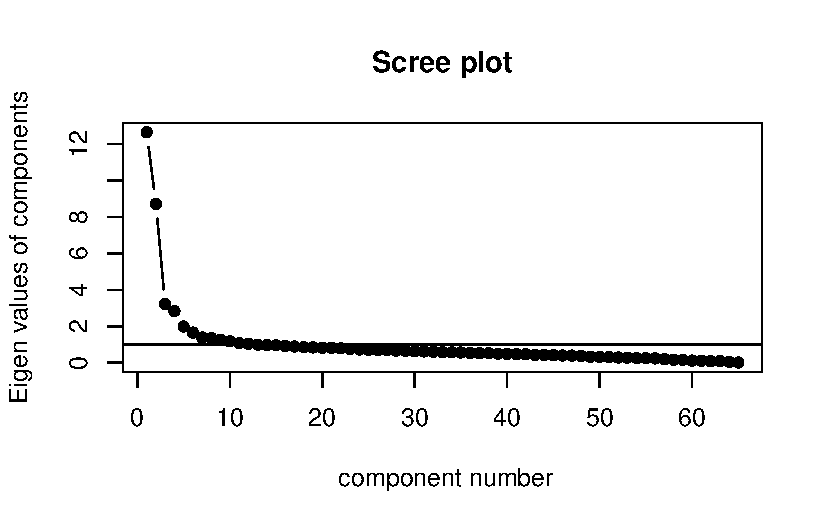
\includegraphics{E_Ch6_Analysis_files/figure-pdf/screeplot-1.pdf}

\begin{Shaded}
\begin{Highlighting}[]
\CommentTok{\#dev.off()}

\CommentTok{\# Perform PCA}
\NormalTok{pca1 }\OtherTok{\textless{}{-}}\NormalTok{ psych}\SpecialCharTok{::}\FunctionTok{principal}\NormalTok{(TxBdata[,}\DecValTok{7}\SpecialCharTok{:}\FunctionTok{ncol}\NormalTok{(TxBdata)], }
                         \AttributeTok{nfactors =} \DecValTok{6}\NormalTok{,}
                         \AttributeTok{rotate =} \StringTok{"none"}\NormalTok{)}
\CommentTok{\#pca1$loadings}
\end{Highlighting}
\end{Shaded}

\subsection{Excluding features with low final
communalites}\label{excluding-features-with-low-final-communalites}

We first check whether some feature have extremely low communalities
(see
\href{https://rdrr.io/cran/FactorAssumptions/man/communalities_optimal_solution.htmlhttps://rdrr.io/cran/FactorAssumptions/man/communalities_optimal_solution.html}{https://rdrr.io/cran/FactorAssumptions/man/communalities\_optimal\_solution.html}).

\begin{verbatim}
  STPR   MDNE    HDG  CAUSE   FREQ   THRC    POS   PROG    ACT   DEMO   MDWS 
  0.09   0.17   0.17   0.19   0.22   0.22   0.24   0.26   0.26   0.27   0.28 
   CUZ   COND   QUPR  EXIST   MDCO  NCOMP  OCCUR   TIME ASPECT  TPP3P    AMP 
  0.28   0.28   0.29   0.29   0.31   0.31   0.32   0.32   0.33   0.33   0.34 
    RP  THATD   THSC     EX  FPP1P  PLACE    PIT    VBG   PEAS   MDCA  DOAUX 
  0.34   0.36   0.39   0.43   0.43   0.43   0.45   0.46   0.47   0.48   0.48 
   VBN   JJPR   JJAT   WHSC  SPLIT   EMPH   QUAN MENTAL  TPP3S   PASS   YNQU 
  0.48   0.49   0.49   0.50   0.51   0.53   0.55   0.56   0.56   0.57   0.58 
POLITE     RB     CC    XX0     DT   COMM   WHQU    TTR  FPP1S     IN     LD 
  0.58   0.58   0.58   0.59   0.62   0.62   0.64   0.65   0.67   0.68   0.68 
  FPUH   VPRT   SPP2   BEMA    DMA    VBD    AWL   CONT     NN   VIMP 
  0.70   0.71   0.72   0.74   0.74   0.80   0.85   0.85   0.87   0.90 
\end{verbatim}

As we chose to exclude features with communalities of \textless{} 0.2,
we remove STPR, HDG, MDNE and CAUSE from the dataset to be analysed.

\begin{Shaded}
\begin{Highlighting}[]
\NormalTok{TxBdataforPCA }\OtherTok{\textless{}{-}}\NormalTok{ TxBdata }\SpecialCharTok{|\textgreater{}} 
  \FunctionTok{select}\NormalTok{(}\SpecialCharTok{{-}}\FunctionTok{c}\NormalTok{(STPR, MDNE, HDG, CAUSE))}
\end{Highlighting}
\end{Shaded}

The overall MSA value of the dataset is now 0.88. None of the remaining
features have individual MSA values below 0.5:

\begin{Shaded}
\begin{Highlighting}[]
\NormalTok{kmo3}\SpecialCharTok{$}\NormalTok{MSAi[}\FunctionTok{order}\NormalTok{(kmo3}\SpecialCharTok{$}\NormalTok{MSAi)] }\SpecialCharTok{|\textgreater{}}\FunctionTok{round}\NormalTok{(}\DecValTok{2}\NormalTok{)}
\end{Highlighting}
\end{Shaded}

\begin{verbatim}
  MDWS   MDCA    POS   FREQ    VBD  TPP3S   VPRT    ACT     LD   COND     DT 
  0.54   0.64   0.64   0.65   0.65   0.66   0.66   0.67   0.69   0.78   0.79 
  MDCO  TPP3P     RP  NCOMP   VIMP   SPP2  DOAUX MENTAL   WHSC    VBG  THATD 
  0.79   0.81   0.82   0.82   0.82   0.82   0.84   0.85   0.86   0.86   0.86 
 EXIST  FPP1S   COMM     NN     IN   WHQU   DEMO ASPECT   JJAT   THRC     EX 
  0.86   0.87   0.88   0.89   0.89   0.89   0.89   0.89   0.89   0.90   0.90 
 OCCUR   PEAS     CC   YNQU   QUAN    AWL   TIME    XX0  FPP1P    TTR   CONT 
  0.90   0.91   0.91   0.91   0.91   0.92   0.92   0.92   0.92   0.92   0.93 
  PROG   BEMA  SPLIT   PASS   JJPR   THSC     RB   QUPR    AMP   FPUH    PIT 
  0.93   0.93   0.93   0.94   0.94   0.95   0.95   0.95   0.95   0.95   0.95 
   VBN    DMA POLITE    CUZ   EMPH  PLACE 
  0.95   0.96   0.96   0.96   0.96   0.97 
\end{verbatim}

The final number of linguistic features entered in the intra-textbook
model of linguistic variation is 61.

\section{Testing the effect of rotating the
components}\label{testing-the-effect-of-rotating-the-components}

This chunk was used when considering whether or not to rotate the
components (see methods section). Ultimately, the components were not
rotated.

\begin{Shaded}
\begin{Highlighting}[]
\CommentTok{\# Comparing a rotated vs. a non{-}rotated solution}

\CommentTok{\#TxBdata \textless{}{-} readRDS(here("data", "processed", "TxBdataforPCA.rds"))}

\CommentTok{\# No rotation}
\NormalTok{pca2 }\OtherTok{\textless{}{-}}\NormalTok{ psych}\SpecialCharTok{::}\FunctionTok{principal}\NormalTok{(TxBdata[,}\DecValTok{7}\SpecialCharTok{:}\FunctionTok{ncol}\NormalTok{(TxBdata)], }
                         \AttributeTok{nfactors =} \DecValTok{6}\NormalTok{, }
                         \AttributeTok{rotate =} \StringTok{"none"}\NormalTok{)}

\NormalTok{pca2}\SpecialCharTok{$}\NormalTok{loadings}

\FunctionTok{biplot.psych}\NormalTok{(pca2, }
             \AttributeTok{vars =} \ConstantTok{TRUE}\NormalTok{, }
             \AttributeTok{choose=}\FunctionTok{c}\NormalTok{(}\DecValTok{1}\NormalTok{,}\DecValTok{2}\NormalTok{),}
\NormalTok{             )}

\CommentTok{\# Promax rotation}
\NormalTok{pca2.rotated }\OtherTok{\textless{}{-}}\NormalTok{ psych}\SpecialCharTok{::}\FunctionTok{principal}\NormalTok{(TxBdata[,}\DecValTok{7}\SpecialCharTok{:}\FunctionTok{ncol}\NormalTok{(TxBdata)], }
                         \AttributeTok{nfactors =} \DecValTok{6}\NormalTok{, }
                         \AttributeTok{rotate =} \StringTok{"promax"}\NormalTok{)}

\CommentTok{\# This summary shows the component correlations which is particularly interesting}
\NormalTok{pca2.rotated}

\NormalTok{pca2.rotated}\SpecialCharTok{$}\NormalTok{loadings}

\FunctionTok{biplot.psych}\NormalTok{(pca2.rotated, }\AttributeTok{vars =} \ConstantTok{TRUE}\NormalTok{, }\AttributeTok{choose=}\FunctionTok{c}\NormalTok{(}\DecValTok{1}\NormalTok{,}\DecValTok{2}\NormalTok{))}
\end{Highlighting}
\end{Shaded}

\section{Principal Component Analysis
(PCA)}\label{principal-component-analysis-pca}

\subsection{Using the full dataset}\label{using-the-full-dataset}

Except outliers removed as part of the data preparation (see Appendix
D).

\begin{Shaded}
\begin{Highlighting}[]
\CommentTok{\# Perform PCA on full data}
\NormalTok{TxBdata }\OtherTok{\textless{}{-}} \FunctionTok{readRDS}\NormalTok{(}\FunctionTok{here}\NormalTok{(}\StringTok{"data"}\NormalTok{, }\StringTok{"processed"}\NormalTok{, }\StringTok{"TxBdataforPCA.rds"}\NormalTok{))}
\end{Highlighting}
\end{Shaded}

\subsection{Using random subsets of the
data}\label{using-random-subsets-of-the-data}

Alternatively, it is possible to conduct the PCA on random subsets of
the data to test the stability of the solution. Re-running this line
will generate a new subset of the TEC texts containing 2/3 of the texts
randomly sampled.

\begin{Shaded}
\begin{Highlighting}[]
\NormalTok{TxBdata }\OtherTok{\textless{}{-}} \FunctionTok{readRDS}\NormalTok{(}\FunctionTok{here}\NormalTok{(}\StringTok{"data"}\NormalTok{, }\StringTok{"processed"}\NormalTok{, }\StringTok{"TxBdataforPCA.rds"}\NormalTok{)) }\SpecialCharTok{|\textgreater{}}
  \FunctionTok{slice\_sample}\NormalTok{(}\AttributeTok{n =} \FunctionTok{round}\NormalTok{(}\DecValTok{1961}\SpecialCharTok{*}\FloatTok{0.6}\NormalTok{), }\AttributeTok{replace =} \ConstantTok{FALSE}\NormalTok{)}

\FunctionTok{nrow}\NormalTok{(TxBdata)}
\NormalTok{TxBdata}\SpecialCharTok{$}\NormalTok{Filename[}\DecValTok{1}\SpecialCharTok{:}\DecValTok{10}\NormalTok{]}
\FunctionTok{nrow}\NormalTok{(TxBdata) }\SpecialCharTok{/}\NormalTok{ (}\FunctionTok{ncol}\NormalTok{(TxBdata)}\SpecialCharTok{{-}}\DecValTok{6}\NormalTok{) }\CommentTok{\# Check that there is enough data to conduct a PCA. This ratio should be at least 5 (see Friginal \& Hardy 2014: 303–304).}
\end{Highlighting}
\end{Shaded}

\subsection{Using specific subsets of the
data}\label{using-specific-subsets-of-the-data}

The following chunk can be used to perform the PCA on a country subset
of the data to test the stability of the solution. See (Le Foll, n.d.)
for a detailed analysis of the subcorpus of textbooks used in Germany.

\begin{Shaded}
\begin{Highlighting}[]
\NormalTok{TxBdata }\OtherTok{\textless{}{-}} \FunctionTok{readRDS}\NormalTok{(}\FunctionTok{here}\NormalTok{(}\StringTok{"data"}\NormalTok{, }\StringTok{"processed"}\NormalTok{, }\StringTok{"TxBdataforPCA.rds"}\NormalTok{)) }\SpecialCharTok{|\textgreater{}}
  \CommentTok{\#filter(Country == "France")}
  \CommentTok{\#filter(Country == "Germany")}
  \FunctionTok{filter}\NormalTok{(Country }\SpecialCharTok{==} \StringTok{"Spain"}\NormalTok{)}

\FunctionTok{nrow}\NormalTok{(TxBdata)}
\NormalTok{TxBdata}\SpecialCharTok{$}\NormalTok{Filename[}\DecValTok{1}\SpecialCharTok{:}\DecValTok{10}\NormalTok{] }\CommentTok{\# Check data}
\FunctionTok{nrow}\NormalTok{(TxBdata) }\SpecialCharTok{/}\NormalTok{ (}\FunctionTok{ncol}\NormalTok{(TxBdata)}\SpecialCharTok{{-}}\DecValTok{6}\NormalTok{) }\CommentTok{\# Check that there is enough data to conduct a PCA. This should be \textgreater{} 5 (see Friginal \& Hardy 2014: 303–304).}
\end{Highlighting}
\end{Shaded}

\subsection{Performing the PCA}\label{performing-the-pca}

We perform the PCA using the \texttt{prcomp} function and print a
summary of the results.

\begin{Shaded}
\begin{Highlighting}[]
\NormalTok{pca }\OtherTok{\textless{}{-}} \FunctionTok{prcomp}\NormalTok{(TxBdata[,}\DecValTok{7}\SpecialCharTok{:}\FunctionTok{ncol}\NormalTok{(TxBdata)], }\AttributeTok{scale.=}\ConstantTok{FALSE}\NormalTok{, }\AttributeTok{rank. =} \DecValTok{6}\NormalTok{) }\CommentTok{\# All quantitative variables for all TxB files except outliers}
\NormalTok{register  }\OtherTok{\textless{}{-}} \FunctionTok{factor}\NormalTok{(TxBdata[,}\StringTok{"Register"}\NormalTok{]) }\CommentTok{\# Register}
\NormalTok{level }\OtherTok{\textless{}{-}} \FunctionTok{factor}\NormalTok{(TxBdata[,}\StringTok{"Level"}\NormalTok{]) }\CommentTok{\# Textbook proficiency level}

\CommentTok{\# summary(register)}
\CommentTok{\# summary(level)}
\FunctionTok{summary}\NormalTok{(pca)}
\end{Highlighting}
\end{Shaded}

\begin{verbatim}
Importance of first k=6 (out of 61) components:
                          PC1    PC2     PC3     PC4     PC5     PC6
Standard deviation     2.1693 1.7776 1.08902 1.00207 0.84288 0.76792
Proportion of Variance 0.2108 0.1416 0.05313 0.04499 0.03183 0.02642
Cumulative Proportion  0.2108 0.3524 0.40553 0.45051 0.48234 0.50876
\end{verbatim}

\section{Plotting PCA results}\label{plotting-pca-results}

\subsection{3D plots}\label{d-plots}

The following chunk can be used to create projections of TEC texts on
three dimensions of the model. These plots cannot be rendered in two
dimensions and are therefore not generated in the present document. For
more information on the \texttt{pca3d} library, see:
\url{https://cran.r-project.org/web/packages/pca3d/vignettes/pca3d.pdf}.

\begin{Shaded}
\begin{Highlighting}[]
\FunctionTok{library}\NormalTok{(pca3d) }\CommentTok{\# For 3{-}D plots}

\NormalTok{col }\OtherTok{\textless{}{-}}\NormalTok{ palette[}\FunctionTok{c}\NormalTok{(}\DecValTok{1}\SpecialCharTok{:}\DecValTok{3}\NormalTok{,}\DecValTok{8}\NormalTok{,}\DecValTok{7}\NormalTok{)] }\CommentTok{\# without poetry}
\FunctionTok{names}\NormalTok{(col) }\OtherTok{\textless{}{-}} \FunctionTok{c}\NormalTok{(}\StringTok{"Conversation"}\NormalTok{, }\StringTok{"Fiction"}\NormalTok{, }\StringTok{"Informative"}\NormalTok{, }\StringTok{"Instructional"}\NormalTok{, }\StringTok{"Personal"}\NormalTok{)}
\NormalTok{scales}\SpecialCharTok{::}\FunctionTok{show\_col}\NormalTok{(col) }\CommentTok{\# Check colours}

\FunctionTok{pca3d}\NormalTok{(pca, }
      \AttributeTok{group =}\NormalTok{ register,}
      \AttributeTok{components =} \DecValTok{1}\SpecialCharTok{:}\DecValTok{3}\NormalTok{,}
      \CommentTok{\#components = 4:6,}
      \AttributeTok{show.ellipses=}\ConstantTok{FALSE}\NormalTok{, }
      \AttributeTok{ellipse.ci=}\FloatTok{0.75}\NormalTok{,}
      \AttributeTok{show.plane=}\ConstantTok{FALSE}\NormalTok{,}
      \AttributeTok{col =}\NormalTok{ col,}
      \AttributeTok{shape =} \StringTok{"sphere"}\NormalTok{,}
      \AttributeTok{radius =} \DecValTok{1}\NormalTok{,}
      \AttributeTok{legend =} \StringTok{"right"}\NormalTok{)}

\FunctionTok{snapshotPCA3d}\NormalTok{(}\FunctionTok{here}\NormalTok{(}\StringTok{"plots"}\NormalTok{, }\StringTok{"PCA\_TxB\_3Dsnapshot.png"}\NormalTok{))}

\FunctionTok{names}\NormalTok{(col) }\OtherTok{\textless{}{-}} \FunctionTok{c}\NormalTok{(}\StringTok{"C"}\NormalTok{, }\StringTok{"B"}\NormalTok{, }\StringTok{"E"}\NormalTok{, }\StringTok{"A"}\NormalTok{, }\StringTok{"D"}\NormalTok{) }\CommentTok{\# To colour the dots according to the profiency level of the textbooks}
\FunctionTok{pca3d}\NormalTok{(pca, }
      \AttributeTok{components =} \DecValTok{4}\SpecialCharTok{:}\DecValTok{6}\NormalTok{,}
      \AttributeTok{group =}\NormalTok{ level,}
      \AttributeTok{show.ellipses=}\ConstantTok{FALSE}\NormalTok{, }
      \AttributeTok{ellipse.ci=}\FloatTok{0.75}\NormalTok{,}
      \AttributeTok{show.plane=}\ConstantTok{FALSE}\NormalTok{,}
      \AttributeTok{col =}\NormalTok{ col,}
      \AttributeTok{shape =} \StringTok{"sphere"}\NormalTok{,}
      \AttributeTok{radius =} \FloatTok{0.8}\NormalTok{,}
      \AttributeTok{legend =} \StringTok{"right"}\NormalTok{)}
\end{Highlighting}
\end{Shaded}

\section{Two-dimensional plots
(biplots)}\label{two-dimensional-plots-biplots}

These plots were generated using the \texttt{PCAtools} package, which
requires the data to be formatted in a rather unconventional way so it
needs to wrangled first.

\subsection{Data wrangling for
PCAtools}\label{data-wrangling-for-pcatools}

\begin{Shaded}
\begin{Highlighting}[]
\CommentTok{\#TxBdata \textless{}{-} readRDS(here("data", "processed", "TxBdataforPCA.rds"))}

\NormalTok{TxBdata2meta }\OtherTok{\textless{}{-}}\NormalTok{ TxBdata[,}\DecValTok{1}\SpecialCharTok{:}\DecValTok{6}\NormalTok{]}
\FunctionTok{rownames}\NormalTok{(TxBdata2meta) }\OtherTok{\textless{}{-}}\NormalTok{ TxBdata2meta}\SpecialCharTok{$}\NormalTok{Filename}
\NormalTok{TxBdata2meta }\OtherTok{\textless{}{-}}\NormalTok{ TxBdata2meta }\SpecialCharTok{|\textgreater{}} \FunctionTok{select}\NormalTok{(}\SpecialCharTok{{-}}\NormalTok{Filename)}
\CommentTok{\#head(TxBdata2meta)}

\NormalTok{TxBdata2 }\OtherTok{=}\NormalTok{ TxBdata}
\FunctionTok{rownames}\NormalTok{(TxBdata2) }\OtherTok{\textless{}{-}}\NormalTok{ TxBdata2}\SpecialCharTok{$}\NormalTok{Filename}
\NormalTok{TxBdata2num }\OtherTok{\textless{}{-}} \FunctionTok{as.data.frame}\NormalTok{(base}\SpecialCharTok{::}\FunctionTok{t}\NormalTok{(TxBdata2[,}\DecValTok{7}\SpecialCharTok{:}\FunctionTok{ncol}\NormalTok{(TxBdata2)]))}
\CommentTok{\#TxBdata2num[1:12,1:3] \# Check sanity of data}

\NormalTok{p }\OtherTok{\textless{}{-}}\NormalTok{ PCAtools}\SpecialCharTok{::}\FunctionTok{pca}\NormalTok{(TxBdata2num, }
         \AttributeTok{metadata =}\NormalTok{ TxBdata2meta,}
         \AttributeTok{scale =} \ConstantTok{FALSE}\NormalTok{)}
\end{Highlighting}
\end{Shaded}

\subsection{Pairs plot}\label{pairs-plot}

We first produce a scatterplot matrix of all the combinations of the
first six dimensions of the model of intra-textbook variation. Note that
the number before the comma on each axis label shows which principal
component is plotted on that axis; this is followed by the percentage of
the total variance explained by that particular component. The colours
correspond to the text registers.

\begin{Shaded}
\begin{Highlighting}[]
\DocumentationTok{\#\# Colour and shape scheme for all biplots}
\NormalTok{colkey }\OtherTok{=} \FunctionTok{c}\NormalTok{(}\AttributeTok{Conversation=}\StringTok{"\#BD241E"}\NormalTok{, }\AttributeTok{Fiction=}\StringTok{"\#A18A33"}\NormalTok{, }\AttributeTok{Informative=}\StringTok{"\#15274D"}\NormalTok{, }\AttributeTok{Instructional=}\StringTok{"\#F9B921"}\NormalTok{, }\AttributeTok{Personal=}\StringTok{"\#722672"}\NormalTok{)}
\NormalTok{shapekey }\OtherTok{=} \FunctionTok{c}\NormalTok{(}\AttributeTok{A=}\DecValTok{1}\NormalTok{, }\AttributeTok{B=}\DecValTok{2}\NormalTok{, }\AttributeTok{C=}\DecValTok{6}\NormalTok{, }\AttributeTok{D=}\DecValTok{0}\NormalTok{, }\AttributeTok{E=}\DecValTok{5}\NormalTok{)}

\DocumentationTok{\#\# Very slow, open in zoomed out window!}
\CommentTok{\# Add legend manually? Yes (take it from the biplot code below), sadly really the simplest solution, here. Or use Evert\textquotesingle{}s mvar.pairs plot function (though that also requires manual axis annotation).}

\CommentTok{\# png(here("plots", "PCA\_TxB\_pairsplot.png"), width = 12, height= 19, units = "cm", res = 300)}
\NormalTok{PCAtools}\SpecialCharTok{::}\FunctionTok{pairsplot}\NormalTok{(p,}
                 \AttributeTok{triangle =} \ConstantTok{FALSE}\NormalTok{,}
                 \AttributeTok{components =} \DecValTok{1}\SpecialCharTok{:}\DecValTok{6}\NormalTok{,}
                 \AttributeTok{ncol =} \DecValTok{3}\NormalTok{,}
                 \AttributeTok{nrow =} \DecValTok{5}\NormalTok{,}
                 \AttributeTok{pointSize =} \FloatTok{0.8}\NormalTok{,}
                 \AttributeTok{lab =} \ConstantTok{NULL}\NormalTok{, }\CommentTok{\# Otherwise will try to label each data point!}
                 \AttributeTok{colby =} \StringTok{"Register"}\NormalTok{,}
                 \AttributeTok{colkey =}\NormalTok{ colkey,}
                 \AttributeTok{shape =} \StringTok{"Level"}\NormalTok{,}
                 \AttributeTok{shapekey =}\NormalTok{ shapekey,}
                 \AttributeTok{margingaps =} \FunctionTok{unit}\NormalTok{(}\FunctionTok{c}\NormalTok{(}\FloatTok{0.2}\NormalTok{, }\FloatTok{0.2}\NormalTok{, }\FloatTok{0.2}\NormalTok{, }\FloatTok{0.2}\NormalTok{), }\StringTok{"cm"}\NormalTok{),}
                 \AttributeTok{legendPosition =} \StringTok{"none"}\NormalTok{)}
\end{Highlighting}
\end{Shaded}

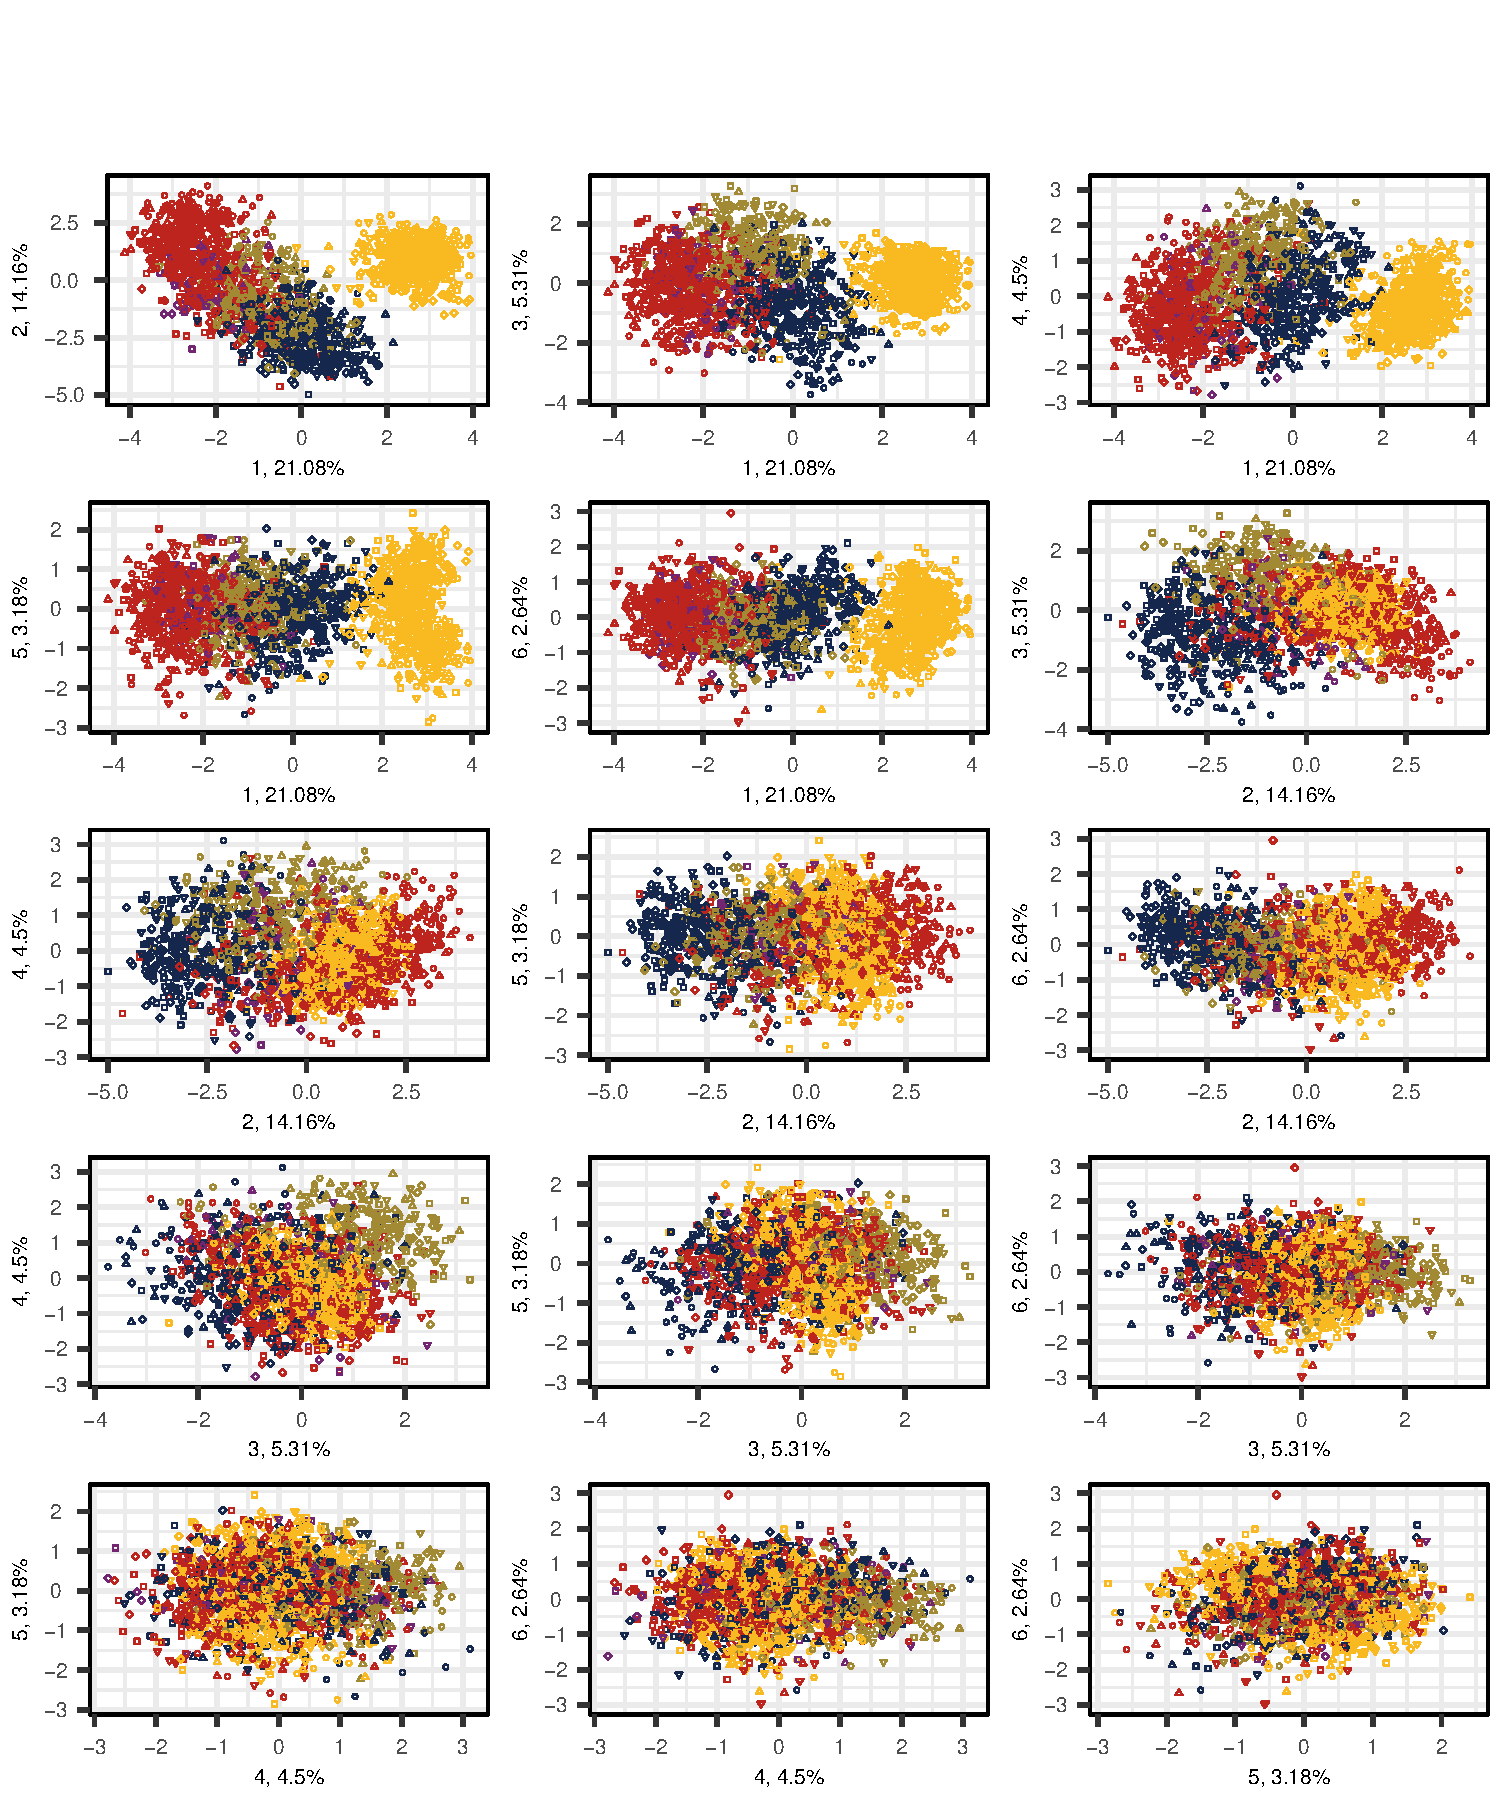
\includegraphics{E_Ch6_Analysis_files/figure-pdf/PCAtools-pairsplots-TxB-1.pdf}

\subsection{Bi-plots}\label{bi-plots}

Then, biplots of the most important dimensions are generated to examine
components more carefully.

\begin{Shaded}
\begin{Highlighting}[]
\NormalTok{colkey }\OtherTok{=} \FunctionTok{c}\NormalTok{(}\AttributeTok{Conversation=}\StringTok{"\#BD241E"}\NormalTok{, }\AttributeTok{Fiction=}\StringTok{"\#A18A33"}\NormalTok{, }\AttributeTok{Informative=}\StringTok{"\#15274D"}\NormalTok{, }\AttributeTok{Instructional=}\StringTok{"\#F9B921"}\NormalTok{, }\AttributeTok{Personal=}\StringTok{"\#722672"}\NormalTok{)}
\NormalTok{shapekey }\OtherTok{=} \FunctionTok{c}\NormalTok{(}\AttributeTok{A=}\DecValTok{1}\NormalTok{, }\AttributeTok{B=}\DecValTok{2}\NormalTok{, }\AttributeTok{C=}\DecValTok{6}\NormalTok{, }\AttributeTok{D=}\DecValTok{0}\NormalTok{, }\AttributeTok{E=}\DecValTok{5}\NormalTok{)}

\CommentTok{\#png(here("plots", "PCA\_TxB\_Biplot\_PC1\_PC2.png"), width = 40, height= 25, units = "cm", res = 300)}
\NormalTok{PCAtools}\SpecialCharTok{::}\FunctionTok{biplot}\NormalTok{(p,}
                 \AttributeTok{x =} \StringTok{"PC1"}\NormalTok{,}
                 \AttributeTok{y =} \StringTok{"PC2"}\NormalTok{,}
                 \AttributeTok{lab =} \ConstantTok{NULL}\NormalTok{, }\CommentTok{\# Otherwise will try to label each data point!}
                 \CommentTok{\#xlim = c(min(p$rotated$PC1){-}0.5, max(p$rotated$PC1)+0.5),}
                 \CommentTok{\#ylim = c(min(p$rotated$PC2){-}0.5, max(p$rotated$PC2)+0.5),}
                 \AttributeTok{colby =} \StringTok{"Register"}\NormalTok{,}
                 \AttributeTok{pointSize =} \DecValTok{2}\NormalTok{,}
                 \AttributeTok{colkey =}\NormalTok{ colkey,}
                 \AttributeTok{shape =} \StringTok{"Level"}\NormalTok{,}
                 \AttributeTok{shapekey =}\NormalTok{ shapekey,}
                 \AttributeTok{showLoadings =} \ConstantTok{FALSE}\NormalTok{,}
                 \AttributeTok{ellipse =} \ConstantTok{TRUE}\NormalTok{,}
                 \AttributeTok{axisLabSize =} \DecValTok{22}\NormalTok{,}
                 \AttributeTok{legendPosition =} \StringTok{\textquotesingle{}right\textquotesingle{}}\NormalTok{,}
                 \AttributeTok{legendTitleSize =} \DecValTok{22}\NormalTok{,}
                 \AttributeTok{legendLabSize =} \DecValTok{18}\NormalTok{, }
                 \AttributeTok{legendIconSize =} \DecValTok{7}\NormalTok{) }\SpecialCharTok{+}
  \FunctionTok{theme}\NormalTok{(}\AttributeTok{plot.margin =} \FunctionTok{unit}\NormalTok{(}\FunctionTok{c}\NormalTok{(}\DecValTok{0}\NormalTok{,}\DecValTok{0}\NormalTok{,}\DecValTok{0}\NormalTok{,}\FloatTok{0.2}\NormalTok{), }\StringTok{"cm"}\NormalTok{))}
\end{Highlighting}
\end{Shaded}

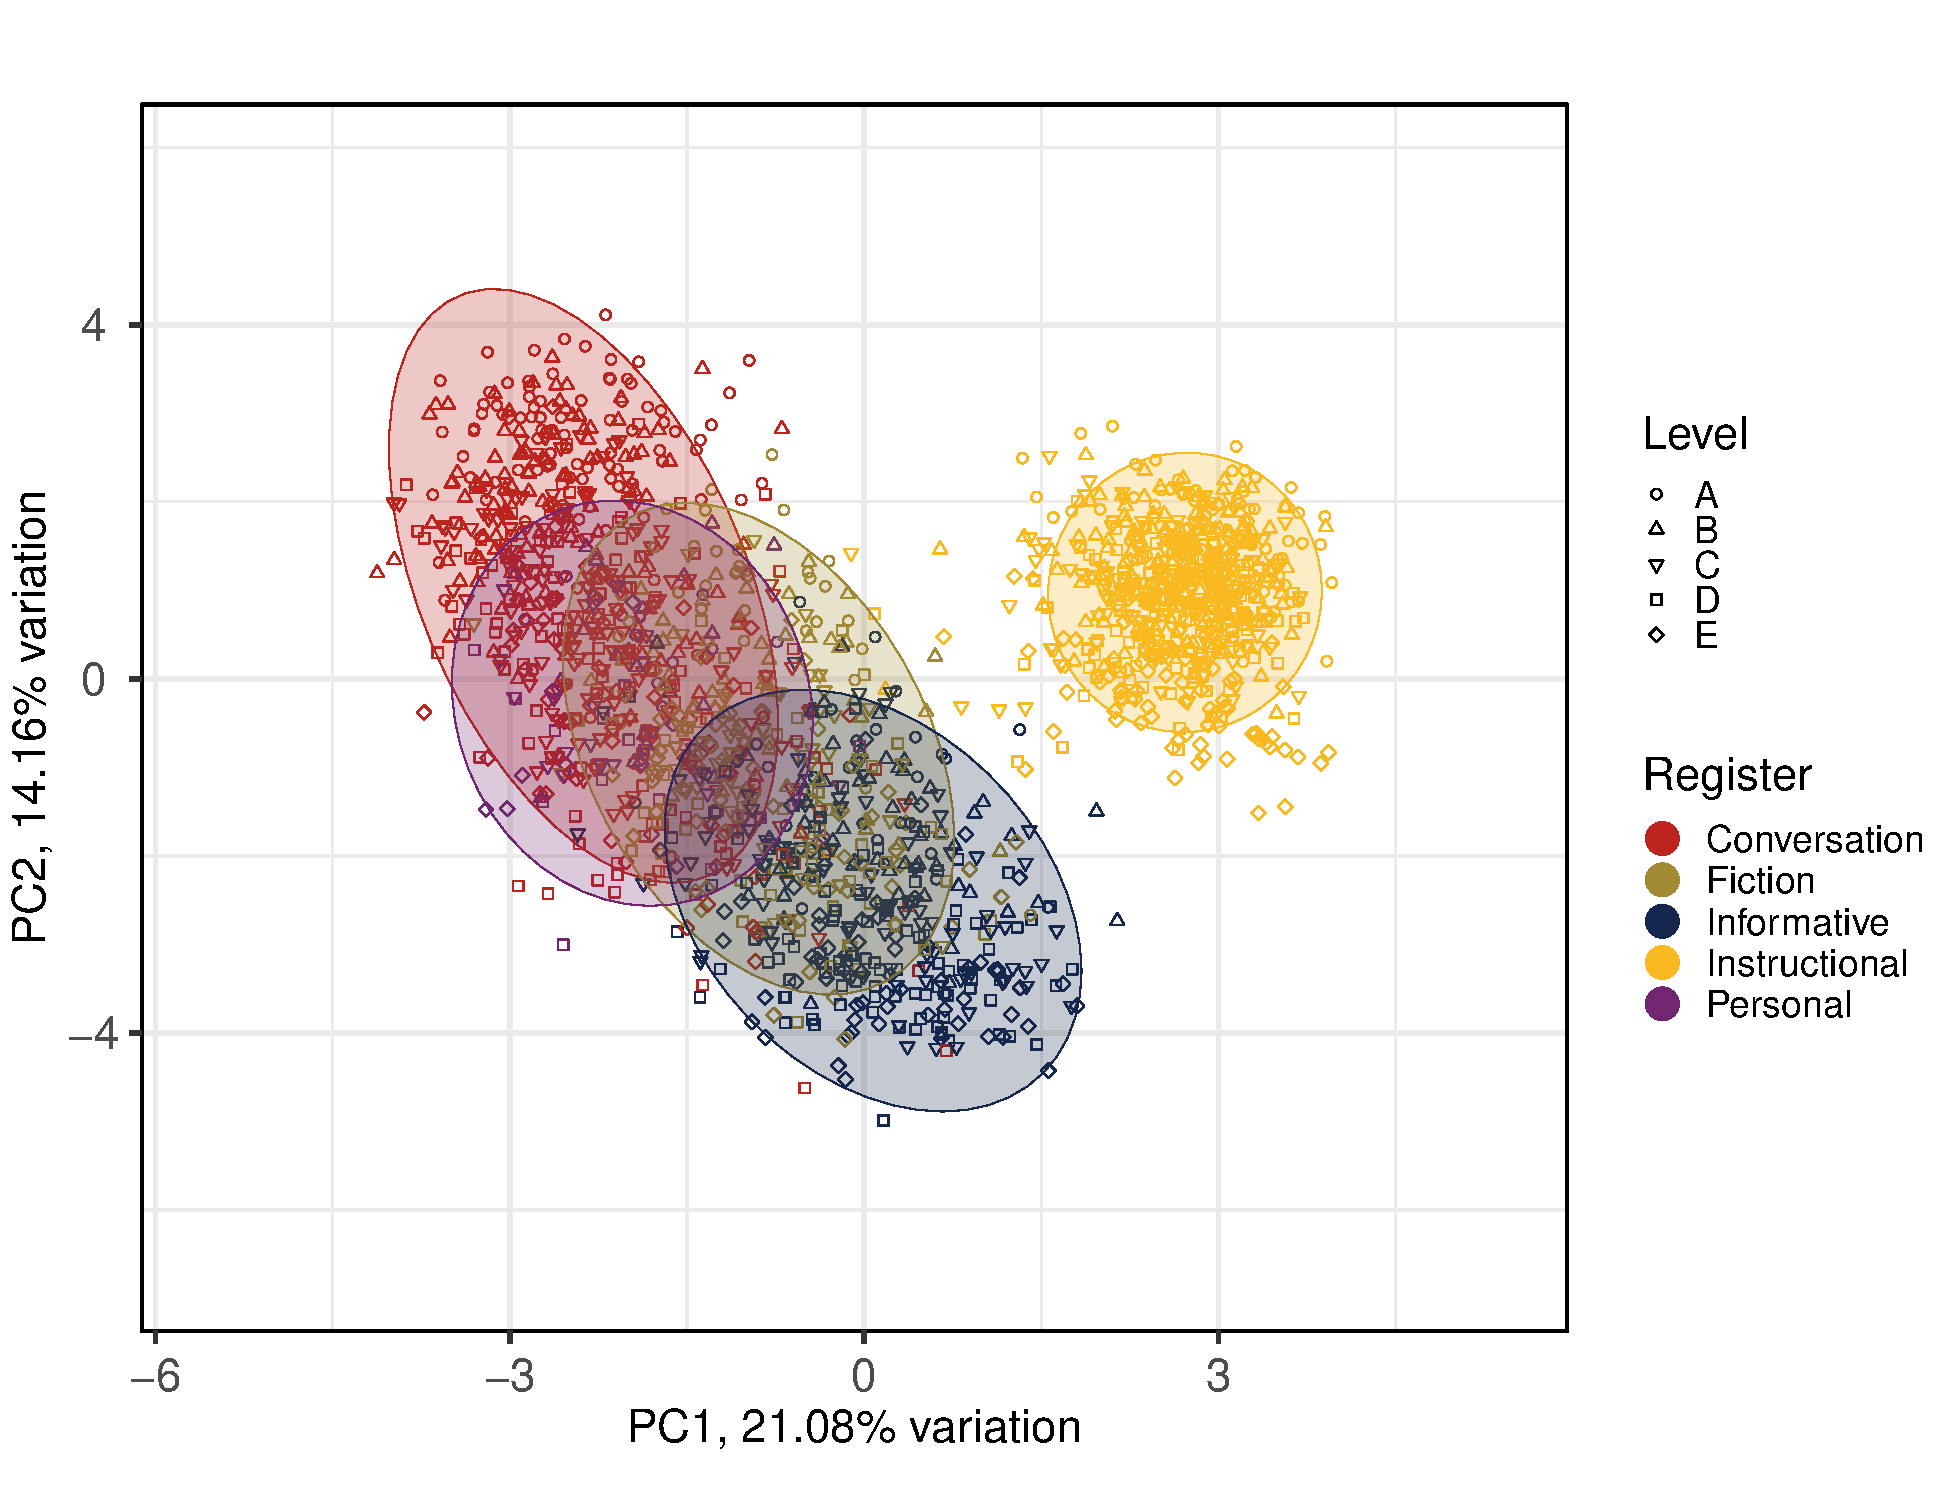
\includegraphics{E_Ch6_Analysis_files/figure-pdf/PCAtools-biplots-TxB-1.pdf}

\begin{Shaded}
\begin{Highlighting}[]
\CommentTok{\#dev.off()}
\CommentTok{\#ggsave(here("plots", "PCA\_TxB\_BiplotPC1\_PC2.svg"), width = 12, height = 10)}

\CommentTok{\# Biplots to examine components more carefully}
\NormalTok{pRegisters }\OtherTok{\textless{}{-}}\NormalTok{ PCAtools}\SpecialCharTok{::}\FunctionTok{biplot}\NormalTok{(p,}
                 \AttributeTok{x =} \StringTok{"PC3"}\NormalTok{,}
                 \AttributeTok{y =} \StringTok{"PC4"}\NormalTok{,}
                 \AttributeTok{lab =} \ConstantTok{NULL}\NormalTok{, }\CommentTok{\# Otherwise will try to label each data point!}
                 \AttributeTok{colby =} \StringTok{"Register"}\NormalTok{,}
                 \AttributeTok{pointSize =} \DecValTok{2}\NormalTok{,}
                 \AttributeTok{colkey =}\NormalTok{ colkey,}
                 \AttributeTok{shape =} \StringTok{"Level"}\NormalTok{,}
                 \AttributeTok{shapekey =}\NormalTok{ shapekey,}
                 \AttributeTok{showLoadings =} \ConstantTok{FALSE}\NormalTok{,}
                 \AttributeTok{ellipse =} \ConstantTok{TRUE}\NormalTok{,}
                 \AttributeTok{legendPosition =} \StringTok{\textquotesingle{}right\textquotesingle{}}\NormalTok{,}
                 \AttributeTok{legendTitleSize =} \DecValTok{22}\NormalTok{,}
                 \AttributeTok{legendLabSize =} \DecValTok{18}\NormalTok{, }
                 \AttributeTok{legendIconSize =} \DecValTok{7}\NormalTok{) }\SpecialCharTok{+}
  \FunctionTok{theme}\NormalTok{(}\AttributeTok{plot.margin =} \FunctionTok{unit}\NormalTok{(}\FunctionTok{c}\NormalTok{(}\DecValTok{0}\NormalTok{,}\DecValTok{0}\NormalTok{,}\DecValTok{0}\NormalTok{,}\FloatTok{0.2}\NormalTok{), }\StringTok{"cm"}\NormalTok{))}

\CommentTok{\#ggsave(here("plots", "PCA\_TxB\_BiplotPC3\_PC4.svg"), width = 12, height = 10)}

\CommentTok{\# Biplots to examine components more carefully}
\NormalTok{pRegisters2 }\OtherTok{\textless{}{-}}\NormalTok{ PCAtools}\SpecialCharTok{::}\FunctionTok{biplot}\NormalTok{(p,}
                 \AttributeTok{x =} \StringTok{"PC5"}\NormalTok{,}
                 \AttributeTok{y =} \StringTok{"PC6"}\NormalTok{,}
                 \AttributeTok{lab =} \ConstantTok{NULL}\NormalTok{, }\CommentTok{\# Otherwise will try to label each data point!}
                 \AttributeTok{colby =} \StringTok{"Register"}\NormalTok{,}
                 \AttributeTok{pointSize =} \DecValTok{2}\NormalTok{,}
                 \AttributeTok{colkey =}\NormalTok{ colkey,}
                 \AttributeTok{shape =} \StringTok{"Level"}\NormalTok{,}
                 \AttributeTok{shapekey =}\NormalTok{ shapekey,}
                 \AttributeTok{showLoadings =} \ConstantTok{FALSE}\NormalTok{,}
                 \AttributeTok{ellipse =} \ConstantTok{TRUE}\NormalTok{,}
                 \AttributeTok{legendPosition =} \StringTok{\textquotesingle{}right\textquotesingle{}}\NormalTok{,}
                 \AttributeTok{legendTitleSize =} \DecValTok{22}\NormalTok{,}
                 \AttributeTok{legendLabSize =} \DecValTok{18}\NormalTok{, }
                 \AttributeTok{legendIconSize =} \DecValTok{7}\NormalTok{) }\SpecialCharTok{+}
  \FunctionTok{theme}\NormalTok{(}\AttributeTok{plot.margin =} \FunctionTok{unit}\NormalTok{(}\FunctionTok{c}\NormalTok{(}\DecValTok{0}\NormalTok{,}\DecValTok{0}\NormalTok{,}\DecValTok{0}\NormalTok{,}\FloatTok{0.2}\NormalTok{), }\StringTok{"cm"}\NormalTok{))}

\CommentTok{\#ggsave(here("plots", "PCA\_TxB\_BiplotPC5\_PC6.svg"), width = 12, height = 10)}
\end{Highlighting}
\end{Shaded}

Changing the colour of the points and the ellipses to represent the
texts' target proficiency levels instead of the register allows for a
different interpretation of the model.

\begin{Shaded}
\begin{Highlighting}[]
\CommentTok{\# Inverted keys for the biplots with ellipses for Level rather than Register}
\NormalTok{colkeyLevels }\OtherTok{=} \FunctionTok{c}\NormalTok{(}\AttributeTok{A=}\StringTok{"\#F9B921"}\NormalTok{, }\AttributeTok{B=}\StringTok{"\#A18A33"}\NormalTok{, }\AttributeTok{C=}\StringTok{"\#BD241E"}\NormalTok{, }\AttributeTok{D=}\StringTok{"\#722672"}\NormalTok{, }\AttributeTok{E=}\StringTok{"\#15274D"}\NormalTok{)}
\NormalTok{shapekeyLevels }\OtherTok{=} \FunctionTok{c}\NormalTok{(}\AttributeTok{Conversation=}\DecValTok{1}\NormalTok{, }\AttributeTok{Fiction=}\DecValTok{2}\NormalTok{, }\AttributeTok{Informative=}\DecValTok{6}\NormalTok{, }\AttributeTok{Instructional=}\DecValTok{0}\NormalTok{, }\AttributeTok{Personal=}\DecValTok{5}\NormalTok{)}

\NormalTok{pLevels }\OtherTok{\textless{}{-}}\NormalTok{ PCAtools}\SpecialCharTok{::}\FunctionTok{biplot}\NormalTok{(p,}
                 \AttributeTok{x =} \StringTok{"PC3"}\NormalTok{,}
                 \AttributeTok{y =} \StringTok{"PC4"}\NormalTok{,}
                 \AttributeTok{lab =} \ConstantTok{NULL}\NormalTok{, }\CommentTok{\# Otherwise will try to label each data point!}
                 \CommentTok{\#xlim = c(min(p$rotated$PC1){-}0.5, max(p$rotated$PC1)+0.5),}
                 \CommentTok{\#ylim = c(min(p$rotated$PC2){-}0.5, max(p$rotated$PC2)+0.5),}
                 \AttributeTok{colby =} \StringTok{"Level"}\NormalTok{,}
                 \AttributeTok{pointSize =} \DecValTok{2}\NormalTok{,}
                 \AttributeTok{colkey =}\NormalTok{ colkeyLevels,}
                 \AttributeTok{shape =} \StringTok{"Register"}\NormalTok{,}
                 \AttributeTok{shapekey =}\NormalTok{ shapekeyLevels,}
                 \AttributeTok{showLoadings =} \ConstantTok{FALSE}\NormalTok{,}
                 \AttributeTok{ellipse =} \ConstantTok{TRUE}\NormalTok{,}
                 \AttributeTok{legendPosition =} \StringTok{\textquotesingle{}right\textquotesingle{}}\NormalTok{,}
                 \AttributeTok{legendTitleSize =} \DecValTok{22}\NormalTok{,}
                 \AttributeTok{legendLabSize =} \DecValTok{18}\NormalTok{, }
                 \AttributeTok{legendIconSize =} \DecValTok{7}\NormalTok{) }\SpecialCharTok{+}
  \FunctionTok{theme}\NormalTok{(}\AttributeTok{plot.margin =} \FunctionTok{unit}\NormalTok{(}\FunctionTok{c}\NormalTok{(}\DecValTok{0}\NormalTok{,}\DecValTok{0}\NormalTok{,}\DecValTok{0}\NormalTok{,}\FloatTok{0.2}\NormalTok{), }\StringTok{"cm"}\NormalTok{))}
\CommentTok{\#ggsave(here("plots", "PCA\_TxB\_BiplotPC3\_PC4\_Level.svg"), width = 12, height = 10)}

\NormalTok{pLevels2 }\OtherTok{\textless{}{-}}\NormalTok{ PCAtools}\SpecialCharTok{::}\FunctionTok{biplot}\NormalTok{(p,}
                 \AttributeTok{x =} \StringTok{"PC5"}\NormalTok{,}
                 \AttributeTok{y =} \StringTok{"PC6"}\NormalTok{,}
                 \AttributeTok{lab =} \ConstantTok{NULL}\NormalTok{, }\CommentTok{\# Otherwise will try to label each data point!}
                 \CommentTok{\#xlim = c(min(p$rotated$PC1){-}0.5, max(p$rotated$PC1)+0.5),}
                 \CommentTok{\#ylim = c(min(p$rotated$PC2){-}0.5, max(p$rotated$PC2)+0.5),}
                 \AttributeTok{colby =} \StringTok{"Level"}\NormalTok{,}
                 \AttributeTok{pointSize =} \DecValTok{2}\NormalTok{,}
                 \AttributeTok{colkey =}\NormalTok{ colkeyLevels,}
                 \AttributeTok{shape =} \StringTok{"Register"}\NormalTok{,}
                 \AttributeTok{shapekey =}\NormalTok{ shapekeyLevels,}
                 \AttributeTok{showLoadings =} \ConstantTok{FALSE}\NormalTok{,}
                 \AttributeTok{ellipse =} \ConstantTok{TRUE}\NormalTok{,}
                 \AttributeTok{legendPosition =} \StringTok{\textquotesingle{}right\textquotesingle{}}\NormalTok{,}
                 \AttributeTok{legendTitleSize =} \DecValTok{22}\NormalTok{,}
                 \AttributeTok{legendLabSize =} \DecValTok{18}\NormalTok{, }
                 \AttributeTok{legendIconSize =} \DecValTok{7}\NormalTok{) }\SpecialCharTok{+}
  \FunctionTok{theme}\NormalTok{(}\AttributeTok{plot.margin =} \FunctionTok{unit}\NormalTok{(}\FunctionTok{c}\NormalTok{(}\DecValTok{0}\NormalTok{,}\DecValTok{0}\NormalTok{,}\DecValTok{0}\NormalTok{,}\FloatTok{0.2}\NormalTok{), }\StringTok{"cm"}\NormalTok{))}
\CommentTok{\#ggsave(here("plots", "PCA\_TxB\_BiplotPC5\_PC6\_Level.svg"), width = 12, height = 10)}


\CommentTok{\# Display and save the two different representations of data points on PC2 and PC3 using the \{patchwork\} package}
\NormalTok{pRegisters }\SpecialCharTok{/}\NormalTok{ pLevels}
\end{Highlighting}
\end{Shaded}

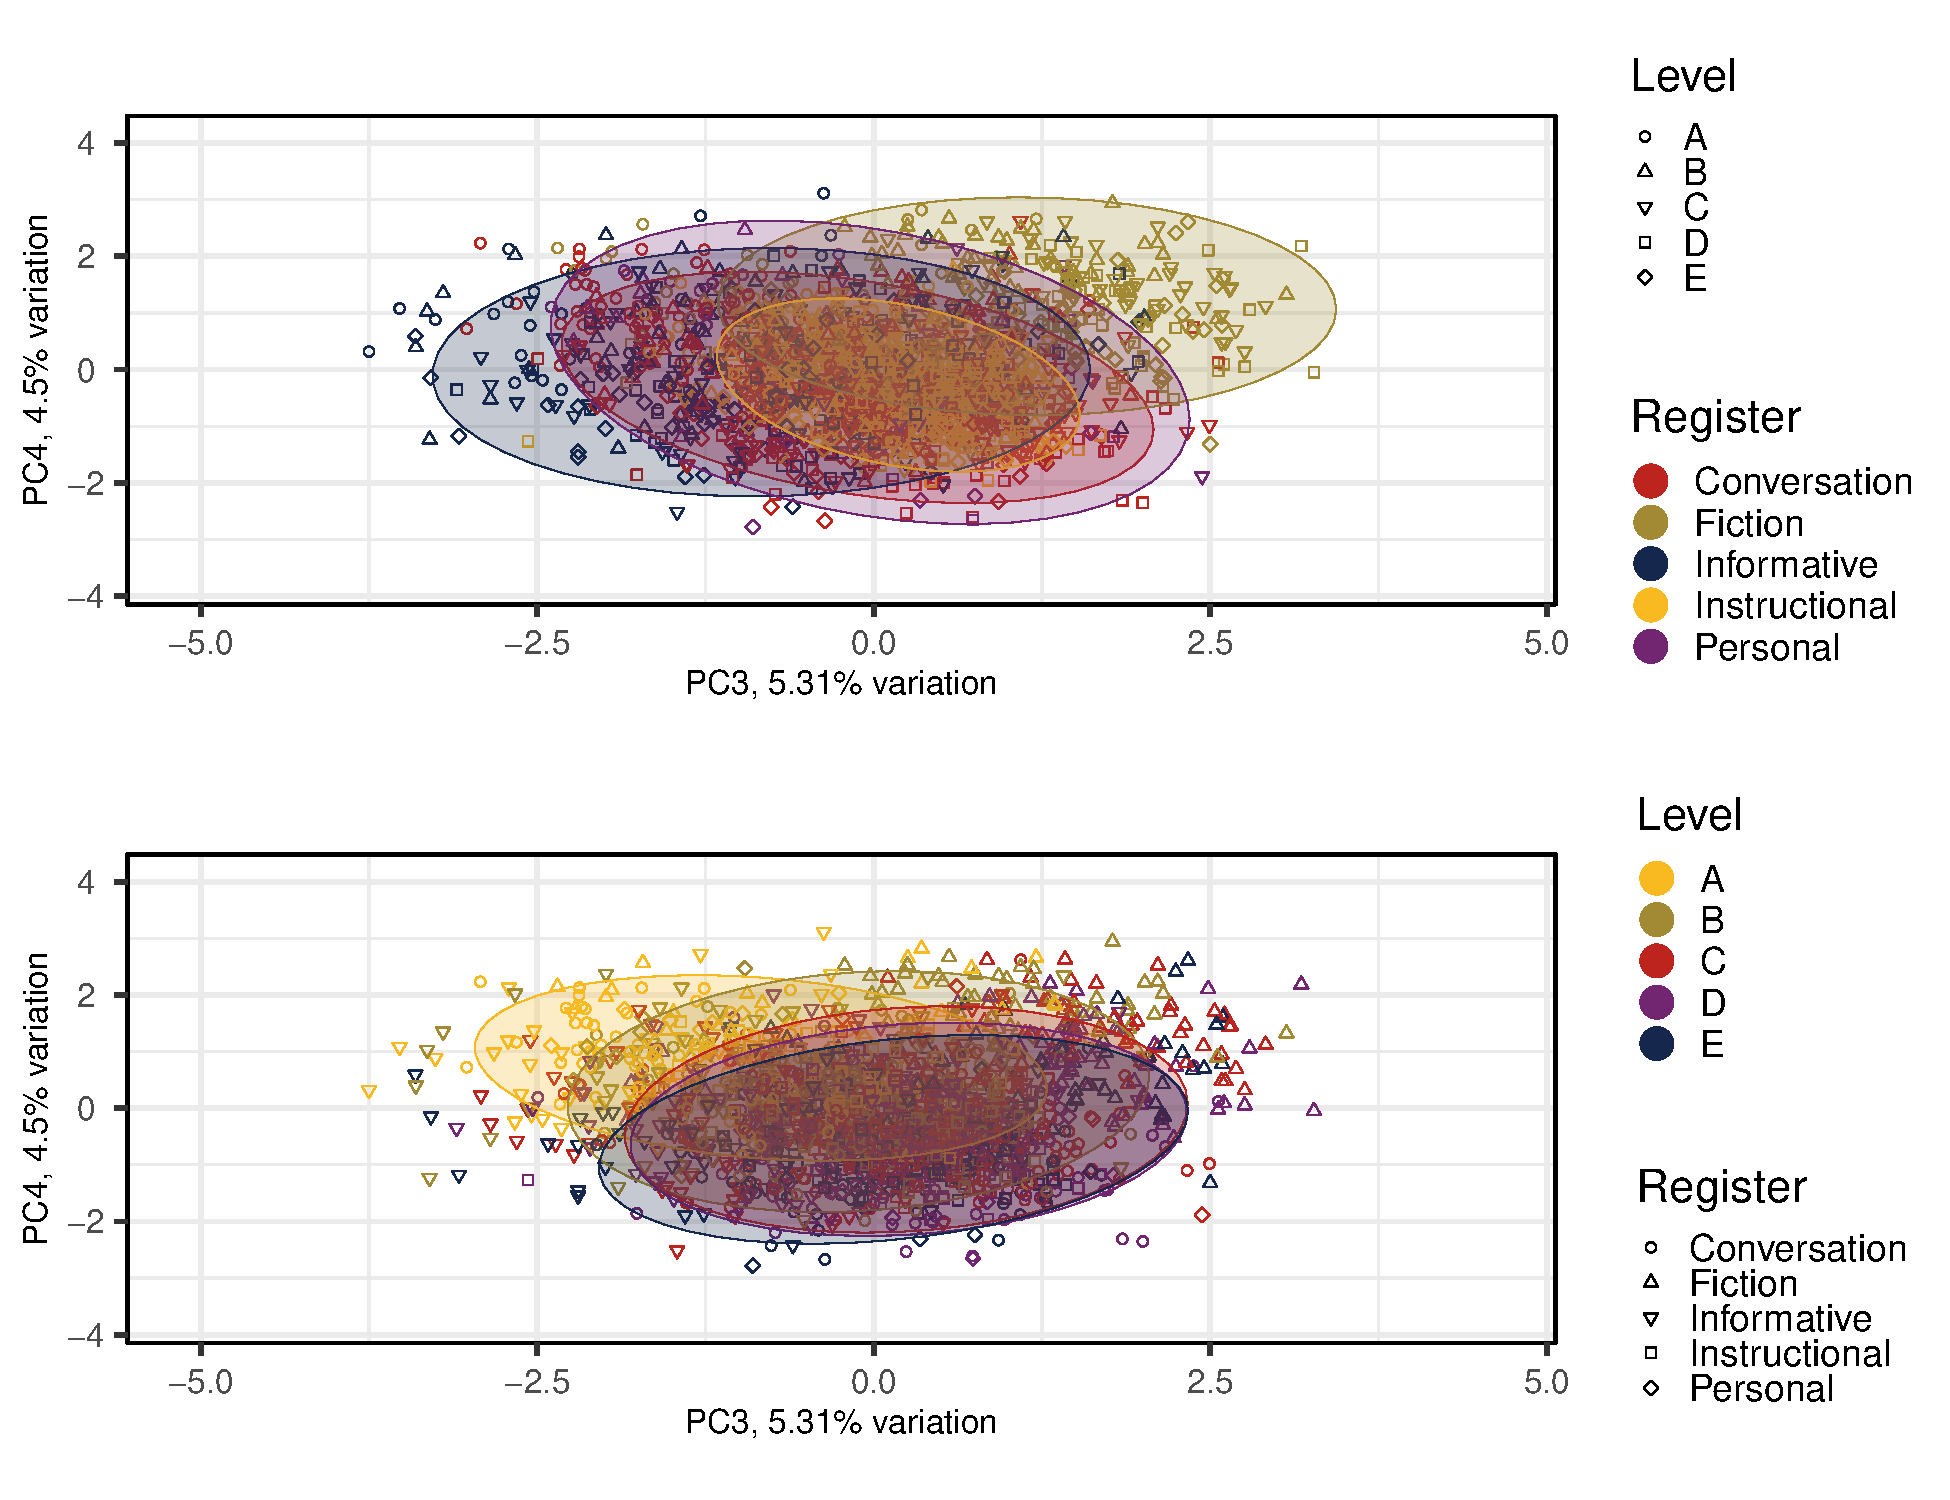
\includegraphics{E_Ch6_Analysis_files/figure-pdf/PCAtools-biplots-TxB-Levels-1.pdf}

\begin{Shaded}
\begin{Highlighting}[]
\CommentTok{\#ggsave(here("plots", "PCA\_TxB\_BiplotPC3\_PC4\_Register\_vs\_Level.svg"), width = 14, height = 20)}

\CommentTok{\# Display and save the two different representations of data points on PC5 and PC6 using the \{patchwork\} package }
\NormalTok{pRegisters2 }\SpecialCharTok{/}\NormalTok{ pLevels2}
\end{Highlighting}
\end{Shaded}

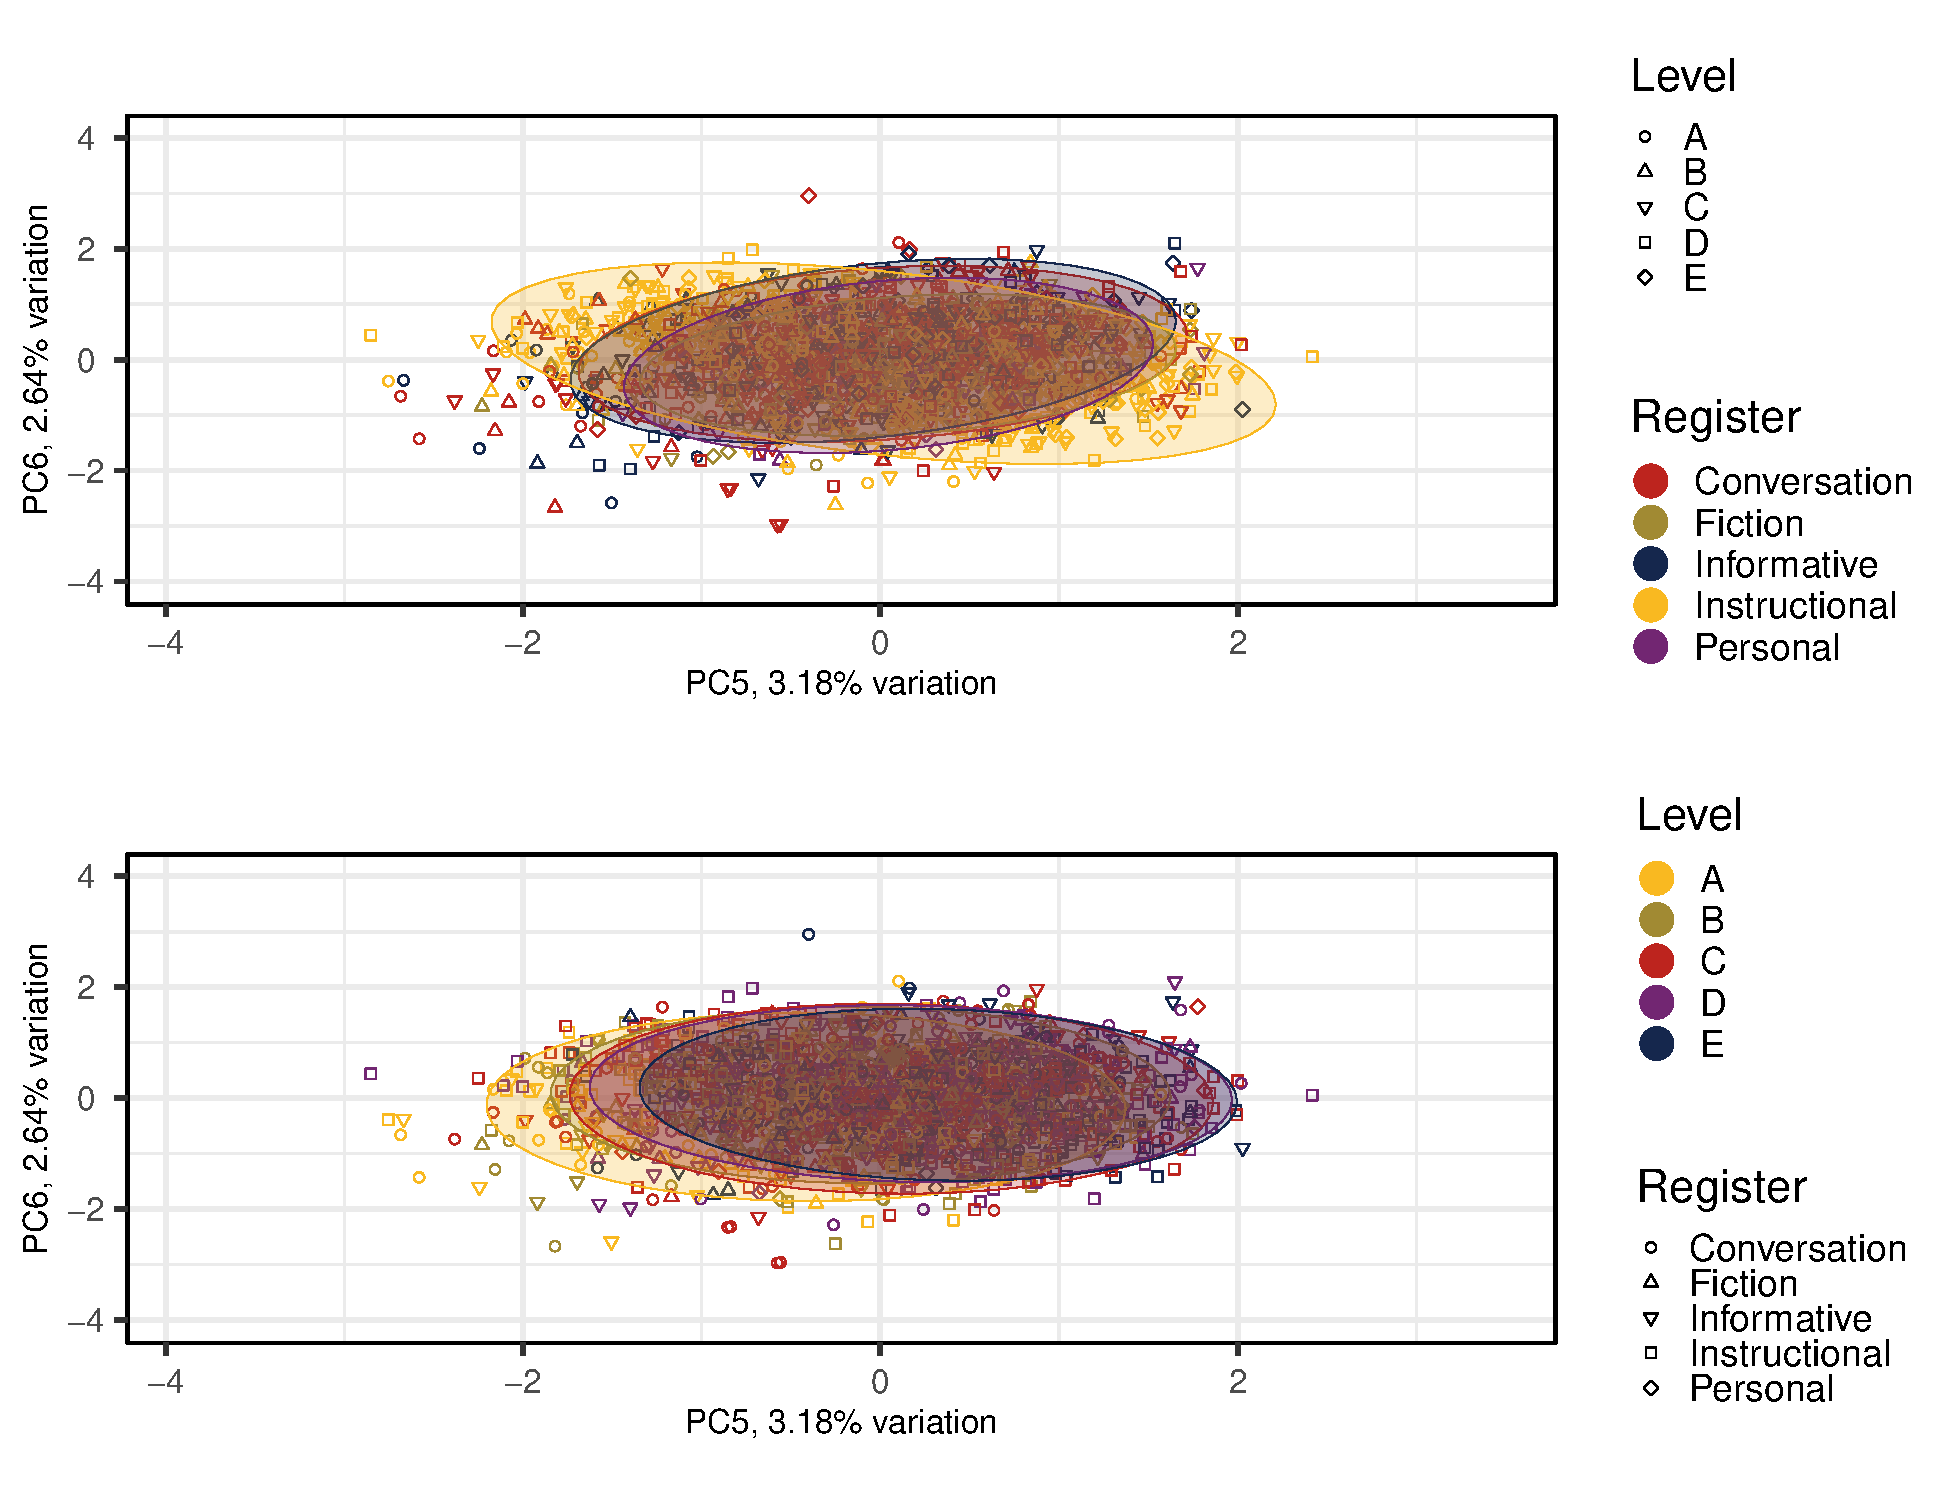
\includegraphics{E_Ch6_Analysis_files/figure-pdf/PCAtools-biplots-TxB-Levels-2.pdf}

\begin{Shaded}
\begin{Highlighting}[]
\CommentTok{\#ggsave(here("plots", "PCA\_TxB\_BiplotPC5\_PC6\_Register\_vs\_Level.svg"), width = 14, height = 20)}
\end{Highlighting}
\end{Shaded}

\section{Feature contributions (loadings) on each
component}\label{feature-contributions-loadings-on-each-component}

\begin{Shaded}
\begin{Highlighting}[]
\CommentTok{\#TxBdata \textless{}{-} readRDS(here("data", "processed", "TxBdataforPCA.rds"))}

\NormalTok{pca }\OtherTok{\textless{}{-}} \FunctionTok{prcomp}\NormalTok{(TxBdata[,}\DecValTok{7}\SpecialCharTok{:}\FunctionTok{ncol}\NormalTok{(TxBdata)], }\AttributeTok{scale.=}\ConstantTok{FALSE}\NormalTok{) }\CommentTok{\# All quantitative variables for all TEC files}

\CommentTok{\# The rotated data that represents the observations / samples is stored in rotated, while the variable loadings are stored in loadings}
\NormalTok{loadings }\OtherTok{\textless{}{-}} \FunctionTok{as.data.frame}\NormalTok{(pca}\SpecialCharTok{$}\NormalTok{rotation[,}\DecValTok{1}\SpecialCharTok{:}\DecValTok{4}\NormalTok{])}
\NormalTok{loadings }\SpecialCharTok{|\textgreater{}} 
  \FunctionTok{round}\NormalTok{(}\DecValTok{2}\NormalTok{) }\SpecialCharTok{|\textgreater{}} 
  \FunctionTok{kable}\NormalTok{()}
\end{Highlighting}
\end{Shaded}

\begin{longtable}[]{@{}lrrrr@{}}
\toprule\noalign{}
& PC1 & PC2 & PC3 & PC4 \\
\midrule\noalign{}
\endhead
\bottomrule\noalign{}
\endlastfoot
ACT & 0.08 & -0.11 & 0.04 & -0.10 \\
AMP & -0.12 & -0.10 & -0.11 & 0.01 \\
ASPECT & 0.10 & -0.05 & 0.14 & -0.01 \\
AWL & 0.22 & -0.16 & -0.12 & -0.13 \\
BEMA & -0.22 & 0.01 & -0.21 & 0.02 \\
CC & 0.05 & -0.21 & -0.19 & 0.00 \\
COMM & 0.20 & 0.09 & 0.14 & -0.04 \\
COND & -0.01 & -0.02 & 0.11 & -0.24 \\
CONT & -0.25 & 0.11 & -0.03 & -0.06 \\
CUZ & -0.09 & -0.13 & -0.06 & -0.02 \\
DEMO & -0.12 & 0.08 & 0.03 & -0.09 \\
DMA & -0.20 & 0.14 & -0.02 & 0.00 \\
DOAUX & -0.01 & 0.20 & 0.05 & -0.15 \\
DT & 0.12 & 0.00 & 0.31 & -0.02 \\
EMPH & -0.19 & -0.02 & 0.06 & -0.14 \\
EX & -0.10 & -0.05 & -0.11 & 0.05 \\
EXIST & -0.02 & -0.15 & -0.09 & -0.09 \\
FPP1P & -0.17 & 0.01 & -0.07 & 0.00 \\
FPP1S & -0.23 & 0.07 & 0.08 & -0.01 \\
FPUH & -0.16 & 0.15 & -0.09 & 0.07 \\
FREQ & -0.03 & -0.05 & 0.01 & -0.10 \\
IN & 0.17 & -0.18 & 0.02 & -0.08 \\
JJAT & -0.06 & -0.18 & 0.04 & -0.21 \\
JJPR & -0.17 & -0.06 & -0.11 & -0.11 \\
LD & 0.16 & -0.03 & -0.26 & -0.01 \\
MDCA & -0.04 & 0.10 & -0.18 & -0.09 \\
MDCO & -0.05 & -0.10 & 0.22 & 0.01 \\
MDWS & -0.07 & -0.01 & 0.05 & -0.16 \\
MENTAL & 0.14 & 0.13 & 0.12 & -0.25 \\
NCOMP & 0.04 & -0.05 & -0.24 & -0.15 \\
NN & 0.20 & -0.09 & -0.29 & 0.11 \\
OCCUR & 0.02 & -0.18 & 0.03 & 0.02 \\
PASS & -0.01 & -0.22 & -0.06 & -0.05 \\
PEAS & -0.06 & -0.17 & 0.13 & -0.13 \\
PIT & -0.19 & -0.04 & -0.06 & -0.06 \\
PLACE & -0.16 & -0.01 & -0.07 & 0.09 \\
POLITE & -0.14 & 0.13 & -0.07 & 0.02 \\
POS & -0.01 & 0.03 & -0.04 & 0.16 \\
PROG & -0.11 & -0.02 & 0.11 & 0.00 \\
QUAN & -0.15 & -0.03 & 0.12 & -0.19 \\
QUPR & -0.10 & -0.05 & 0.16 & -0.11 \\
RB & -0.19 & -0.08 & 0.20 & 0.00 \\
RP & 0.00 & -0.09 & 0.14 & 0.02 \\
SPLIT & -0.11 & -0.18 & 0.02 & -0.16 \\
SPP2 & 0.10 & 0.22 & -0.01 & -0.25 \\
THATD & -0.05 & 0.04 & 0.16 & -0.24 \\
THRC & 0.02 & -0.11 & -0.02 & -0.18 \\
THSC & -0.06 & -0.17 & 0.07 & -0.14 \\
TIME & -0.12 & -0.08 & -0.01 & 0.06 \\
TPP3P & -0.01 & -0.16 & -0.09 & -0.02 \\
TPP3S & -0.06 & -0.11 & 0.13 & 0.30 \\
TTR & -0.04 & -0.26 & -0.05 & -0.01 \\
VBD & -0.08 & -0.20 & 0.23 & 0.30 \\
VBG & 0.04 & -0.18 & 0.00 & -0.22 \\
VBN & 0.03 & -0.18 & -0.07 & -0.04 \\
VIMP & 0.25 & 0.15 & 0.04 & -0.08 \\
VPRT & -0.15 & 0.05 & -0.32 & -0.22 \\
WHQU & 0.11 & 0.23 & 0.00 & -0.09 \\
WHSC & 0.11 & -0.11 & 0.03 & -0.15 \\
XX0 & -0.22 & 0.03 & 0.06 & -0.06 \\
YNQU & -0.03 & 0.23 & 0.00 & -0.08 \\
\end{longtable}

We can go back to the normalised frequencies of the individual features
to compare them across different registers and levels, e.g.:

\begin{Shaded}
\begin{Highlighting}[]
\NormalTok{TxBcounts }\SpecialCharTok{|\textgreater{}} 
  \FunctionTok{group\_by}\NormalTok{(Register, Level) }\SpecialCharTok{|\textgreater{}} 
  \FunctionTok{summarise}\NormalTok{(}\FunctionTok{median}\NormalTok{(NCOMP), }\FunctionTok{MAD}\NormalTok{(NCOMP)) }\SpecialCharTok{|\textgreater{}} 
  \FunctionTok{select}\NormalTok{(}\DecValTok{1}\SpecialCharTok{:}\DecValTok{4}\NormalTok{) }\SpecialCharTok{|\textgreater{}} 
  \FunctionTok{kable}\NormalTok{(}\AttributeTok{digits=}\DecValTok{2}\NormalTok{)}
\end{Highlighting}
\end{Shaded}

\begin{longtable}[]{@{}llrr@{}}
\toprule\noalign{}
Register & Level & median(NCOMP) & MAD(NCOMP) \\
\midrule\noalign{}
\endhead
\bottomrule\noalign{}
\endlastfoot
Conversation & A & 5.69 & 2.79 \\
Conversation & B & 5.48 & 2.66 \\
Conversation & C & 5.32 & 2.58 \\
Conversation & D & 6.18 & 2.91 \\
Conversation & E & 6.21 & 2.62 \\
Fiction & A & 4.14 & 2.34 \\
Fiction & B & 3.96 & 2.17 \\
Fiction & C & 4.05 & 1.86 \\
Fiction & D & 5.05 & 2.34 \\
Fiction & E & 5.05 & 2.16 \\
Informative & A & 8.07 & 2.48 \\
Informative & B & 7.62 & 2.40 \\
Informative & C & 7.49 & 3.16 \\
Informative & D & 7.56 & 2.46 \\
Informative & E & 8.77 & 2.45 \\
Instructional & A & 6.84 & 2.54 \\
Instructional & B & 6.80 & 2.65 \\
Instructional & C & 6.14 & 2.35 \\
Instructional & D & 6.22 & 2.29 \\
Instructional & E & 6.75 & 2.69 \\
Personal & A & 6.72 & 1.42 \\
Personal & B & 4.92 & 2.33 \\
Personal & C & 5.75 & 1.45 \\
Personal & D & 6.46 & 3.19 \\
Personal & E & 8.22 & 3.09 \\
\end{longtable}

Graphs of features display the features with the strongest contributions
to any two dimensions of the model of intra-textbook variation. They are
created using the \texttt{factoextra::fviz\_pca\_var} function.

\begin{Shaded}
\begin{Highlighting}[]
\NormalTok{factoextra}\SpecialCharTok{::}\FunctionTok{fviz\_pca\_var}\NormalTok{(pca,}
             \AttributeTok{axes =} \FunctionTok{c}\NormalTok{(}\DecValTok{1}\NormalTok{,}\DecValTok{2}\NormalTok{),}
             \AttributeTok{select.var =} \FunctionTok{list}\NormalTok{(}\AttributeTok{cos2 =} \FloatTok{0.1}\NormalTok{),}
             \AttributeTok{col.var =} \StringTok{"contrib"}\NormalTok{, }\CommentTok{\# Colour by contributions to the PC}
             \AttributeTok{gradient.cols =} \FunctionTok{c}\NormalTok{(}\StringTok{"\#F9B921"}\NormalTok{, }\StringTok{"\#DB241E"}\NormalTok{, }\StringTok{"\#722672"}\NormalTok{),}
             \AttributeTok{title =} \StringTok{""}\NormalTok{,}
             \AttributeTok{repel =} \ConstantTok{TRUE}\NormalTok{, }\CommentTok{\# Try to avoid too much text overlapping}
             \AttributeTok{ggtheme =}\NormalTok{ ggthemes}\SpecialCharTok{::}\FunctionTok{theme\_few}\NormalTok{())}
\end{Highlighting}
\end{Shaded}

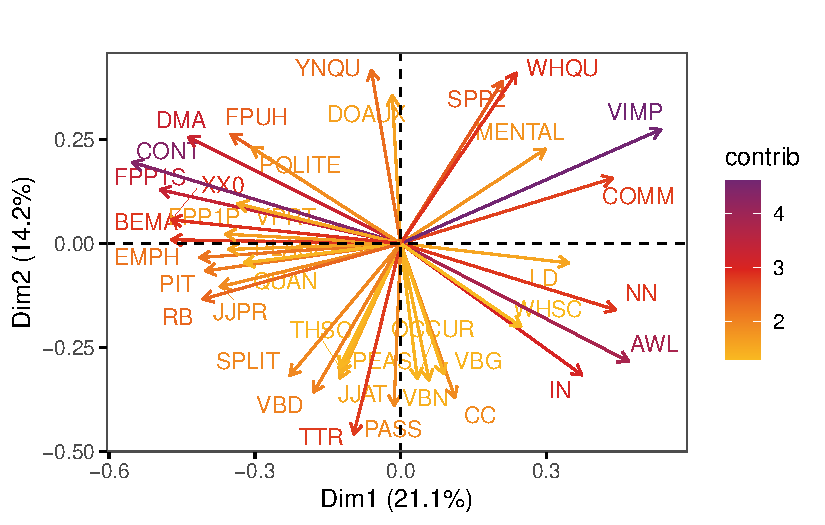
\includegraphics{E_Ch6_Analysis_files/figure-pdf/graphs-of-variables-1.pdf}

\begin{Shaded}
\begin{Highlighting}[]
\CommentTok{\#ggsave(here("plots", "fviz\_pca\_var\_PC1\_PC2.svg"), width = 11, height = 9)}

\NormalTok{factoextra}\SpecialCharTok{::}\FunctionTok{fviz\_pca\_var}\NormalTok{(pca,}
             \AttributeTok{axes =} \FunctionTok{c}\NormalTok{(}\DecValTok{3}\NormalTok{,}\DecValTok{2}\NormalTok{),}
             \AttributeTok{select.var =} \FunctionTok{list}\NormalTok{(}\AttributeTok{contrib =} \DecValTok{30}\NormalTok{),}
             \AttributeTok{col.var =} \StringTok{"contrib"}\NormalTok{, }\CommentTok{\# Colour by contributions to the PC}
             \AttributeTok{gradient.cols =} \FunctionTok{c}\NormalTok{(}\StringTok{"\#F9B921"}\NormalTok{, }\StringTok{"\#DB241E"}\NormalTok{, }\StringTok{"\#722672"}\NormalTok{),}
             \AttributeTok{title =} \StringTok{""}\NormalTok{,}
             \AttributeTok{repel =} \ConstantTok{TRUE}\NormalTok{, }\CommentTok{\# Try to avoid too much text overlapping}
             \AttributeTok{ggtheme =}\NormalTok{ ggthemes}\SpecialCharTok{::}\FunctionTok{theme\_few}\NormalTok{())}
\end{Highlighting}
\end{Shaded}

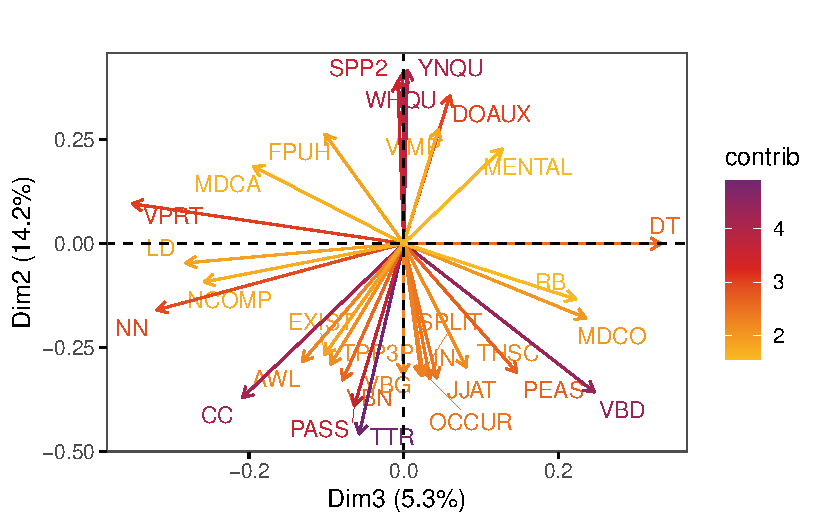
\includegraphics{E_Ch6_Analysis_files/figure-pdf/graphs-of-variables-2.pdf}

\begin{Shaded}
\begin{Highlighting}[]
\CommentTok{\#ggsave(here("plots", "fviz\_pca\_var\_PC3\_PC2.svg"), width = 9, height = 8)}

\NormalTok{factoextra}\SpecialCharTok{::}\FunctionTok{fviz\_pca\_var}\NormalTok{(pca,}
             \AttributeTok{axes =} \FunctionTok{c}\NormalTok{(}\DecValTok{3}\NormalTok{,}\DecValTok{4}\NormalTok{),}
             \AttributeTok{select.var =} \FunctionTok{list}\NormalTok{(}\AttributeTok{contrib =} \DecValTok{30}\NormalTok{),}
             \AttributeTok{col.var =} \StringTok{"contrib"}\NormalTok{, }\CommentTok{\# Colour by contributions to the PC}
             \AttributeTok{gradient.cols =} \FunctionTok{c}\NormalTok{(}\StringTok{"\#F9B921"}\NormalTok{, }\StringTok{"\#DB241E"}\NormalTok{, }\StringTok{"\#722672"}\NormalTok{),}
             \AttributeTok{title =} \StringTok{""}\NormalTok{,}
             \AttributeTok{repel =} \ConstantTok{TRUE}\NormalTok{, }\CommentTok{\# Try to avoid too much text overlapping}
             \AttributeTok{ggtheme =}\NormalTok{ ggthemes}\SpecialCharTok{::}\FunctionTok{theme\_few}\NormalTok{())}
\end{Highlighting}
\end{Shaded}

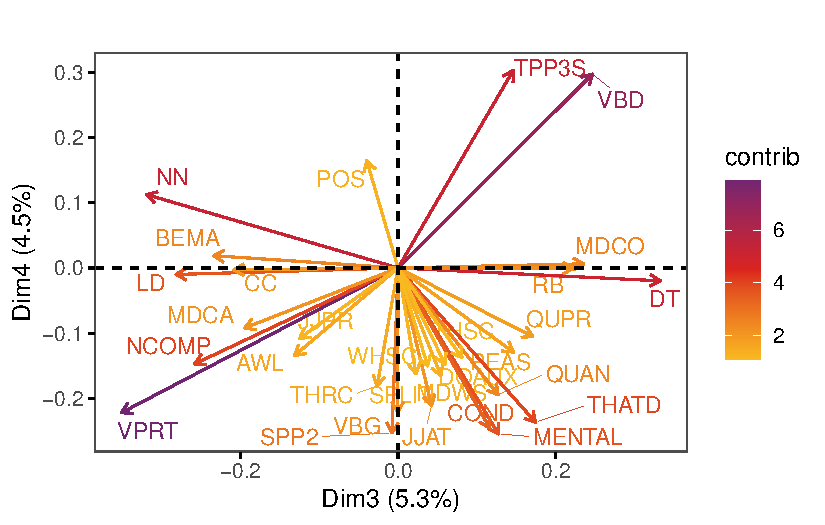
\includegraphics{E_Ch6_Analysis_files/figure-pdf/graphs-of-variables-3.pdf}

\begin{Shaded}
\begin{Highlighting}[]
\CommentTok{\#ggsave(here("plots", "fviz\_pca\_var\_PC3\_PC4.svg"), width = 9, height = 8)}
\end{Highlighting}
\end{Shaded}

\section{Exploring the dimensions of the
model}\label{exploring-the-dimensions-of-the-model}

We begin with some descriptive statistics of the dimension scores.

\begin{Shaded}
\begin{Highlighting}[]
\CommentTok{\# http://www.sthda.com/english/articles/31{-}principal{-}component{-}methods{-}in{-}r{-}practical{-}guide/118{-}principal{-}component{-}analysis{-}in{-}r{-}prcomp{-}vs{-}princomp/\#pca{-}results{-}for{-}variables}

\CommentTok{\#TxBdata \textless{}{-} readRDS(here("data", "processed", "TxBdataforPCA.rds"))}

\NormalTok{pca }\OtherTok{\textless{}{-}} \FunctionTok{prcomp}\NormalTok{(TxBdata[,}\DecValTok{7}\SpecialCharTok{:}\FunctionTok{ncol}\NormalTok{(TxBdata)], }\AttributeTok{scale.=}\ConstantTok{FALSE}\NormalTok{) }\CommentTok{\# All quantitative variables for all TxB files}
\NormalTok{register  }\OtherTok{\textless{}{-}} \FunctionTok{factor}\NormalTok{(TxBdata[,}\StringTok{"Register"}\NormalTok{]) }\CommentTok{\# Register}
\NormalTok{level }\OtherTok{\textless{}{-}} \FunctionTok{factor}\NormalTok{(TxBdata[,}\StringTok{"Level"}\NormalTok{]) }\CommentTok{\# Textbook proficiency level}

\CommentTok{\# summary(register)}
\CommentTok{\# summary(level)}
\CommentTok{\# summary(pca)}

\DocumentationTok{\#\# Access to the PCA results for individual PC}
\CommentTok{\#pca$rotation[,1]}

\NormalTok{res.ind }\OtherTok{\textless{}{-}} \FunctionTok{cbind}\NormalTok{(TxBdata[,}\DecValTok{1}\SpecialCharTok{:}\DecValTok{5}\NormalTok{], }\FunctionTok{as.data.frame}\NormalTok{(pca}\SpecialCharTok{$}\NormalTok{x)[,}\DecValTok{1}\SpecialCharTok{:}\DecValTok{6}\NormalTok{])}

\NormalTok{res.ind }\SpecialCharTok{|\textgreater{}} 
  \FunctionTok{group\_by}\NormalTok{(Register) }\SpecialCharTok{|\textgreater{}} 
  \FunctionTok{summarise\_if}\NormalTok{(is.numeric, mean) }\SpecialCharTok{|\textgreater{}} 
  \FunctionTok{kable}\NormalTok{(}\AttributeTok{digits =} \DecValTok{2}\NormalTok{)}
\end{Highlighting}
\end{Shaded}

\begin{longtable}[]{@{}lrrrrrr@{}}
\toprule\noalign{}
Register & PC1 & PC2 & PC3 & PC4 & PC5 & PC6 \\
\midrule\noalign{}
\endhead
\bottomrule\noalign{}
\endlastfoot
Conversation & -2.29 & 0.93 & -0.14 & -0.27 & -0.02 & 0.06 \\
Fiction & -0.85 & -0.81 & 1.02 & 1.09 & 0.11 & -0.10 \\
Informative & 0.06 & -2.45 & -0.83 & 0.01 & -0.08 & 0.12 \\
Instructional & 2.68 & 0.93 & 0.15 & -0.24 & 0.01 & -0.07 \\
Personal & -1.92 & -0.29 & -0.05 & -0.02 & 0.07 & -0.09 \\
\end{longtable}

\begin{Shaded}
\begin{Highlighting}[]
\NormalTok{res.ind }\SpecialCharTok{|\textgreater{}} 
  \FunctionTok{group\_by}\NormalTok{(Register, Level) }\SpecialCharTok{|\textgreater{}} 
  \FunctionTok{summarise\_if}\NormalTok{(is.numeric, mean) }\SpecialCharTok{|\textgreater{}} 
  \FunctionTok{kable}\NormalTok{(}\AttributeTok{digits =} \DecValTok{2}\NormalTok{)}
\end{Highlighting}
\end{Shaded}

\begin{longtable}[]{@{}llrrrrrr@{}}
\toprule\noalign{}
Register & Level & PC1 & PC2 & PC3 & PC4 & PC5 & PC6 \\
\midrule\noalign{}
\endhead
\bottomrule\noalign{}
\endlastfoot
Conversation & A & -2.39 & 2.39 & -1.23 & 0.71 & -0.45 & -0.01 \\
Conversation & B & -2.54 & 1.72 & -0.25 & 0.04 & -0.14 & 0.13 \\
Conversation & C & -2.25 & 0.70 & 0.18 & -0.41 & 0.09 & -0.02 \\
Conversation & D & -2.10 & -0.08 & 0.28 & -0.73 & 0.17 & 0.09 \\
Conversation & E & -2.13 & -0.14 & 0.07 & -0.98 & 0.16 & 0.17 \\
Fiction & A & -0.95 & 0.85 & -0.54 & 1.48 & -0.31 & -0.46 \\
Fiction & B & -0.89 & -0.14 & 0.95 & 1.78 & -0.06 & -0.03 \\
Fiction & C & -0.98 & -0.81 & 1.62 & 1.23 & 0.26 & -0.16 \\
Fiction & D & -0.71 & -1.57 & 1.27 & 0.72 & 0.21 & -0.01 \\
Fiction & E & -0.80 & -1.45 & 1.16 & 0.56 & 0.25 & -0.01 \\
Informative & A & -0.09 & -1.11 & -1.94 & 0.87 & -0.88 & -0.15 \\
Informative & B & 0.15 & -1.67 & -1.19 & 0.46 & -0.38 & 0.13 \\
Informative & C & -0.02 & -2.37 & -0.68 & -0.03 & -0.06 & -0.01 \\
Informative & D & 0.06 & -2.89 & -0.45 & -0.19 & 0.06 & 0.10 \\
Informative & E & 0.15 & -3.13 & -0.79 & -0.38 & 0.30 & 0.43 \\
Instructional & A & 2.89 & 1.55 & -0.20 & 0.46 & -0.34 & -0.24 \\
Instructional & B & 2.68 & 1.27 & 0.09 & 0.00 & -0.12 & -0.12 \\
Instructional & C & 2.59 & 0.99 & 0.28 & -0.32 & -0.07 & 0.01 \\
Instructional & D & 2.63 & 0.70 & 0.28 & -0.49 & 0.12 & 0.07 \\
Instructional & E & 2.64 & 0.09 & 0.20 & -0.80 & 0.49 & -0.16 \\
Personal & A & -1.84 & 0.53 & -1.11 & 1.21 & -0.31 & 0.12 \\
Personal & B & -1.85 & 0.40 & -0.58 & 0.59 & 0.21 & -0.07 \\
Personal & C & -2.05 & -0.46 & 0.52 & -0.17 & 0.06 & -0.03 \\
Personal & D & -1.89 & -1.05 & 0.45 & -0.63 & 0.39 & -0.06 \\
Personal & E & -1.96 & -0.92 & 0.21 & -1.10 & -0.19 & -0.45 \\
\end{longtable}

The following chunk can be used to search for example texts that are
located in specific areas of the biplots. For example, we can search for
texts that have high scores on Dim3 and low ones on Dim2 to proceed with
a qualitative comparison and analysis of these texts.

\begin{Shaded}
\begin{Highlighting}[]
\NormalTok{res.ind }\SpecialCharTok{|\textgreater{}} 
  \FunctionTok{filter}\NormalTok{(PC3 }\SpecialCharTok{\textgreater{}} \FloatTok{2.5} \SpecialCharTok{\&}\NormalTok{ PC2 }\SpecialCharTok{\textless{}} \SpecialCharTok{{-}}\DecValTok{2}\NormalTok{) }\SpecialCharTok{|\textgreater{}} 
  \FunctionTok{select}\NormalTok{(Filename, PC2, PC3) }\SpecialCharTok{|\textgreater{}} 
  \FunctionTok{kable}\NormalTok{(}\AttributeTok{digits =} \DecValTok{2}\NormalTok{)}
\end{Highlighting}
\end{Shaded}

\begin{longtable}[]{@{}lrr@{}}
\toprule\noalign{}
Filename & PC2 & PC3 \\
\midrule\noalign{}
\endhead
\bottomrule\noalign{}
\endlastfoot
Achievers\_B1\_plus\_Narrative\_0005.txt & -3.88 & 2.60 \\
Solutions\_Intermediate\_Plus\_Spoken\_0018.txt & -2.08 & 2.56 \\
JTT\_3\_Narrative\_0005.txt & -2.85 & 2.76 \\
Achievers\_B2\_Narrative\_00031.txt & -2.61 & 2.59 \\
Access\_4\_Narrative\_0006.txt & -2.19 & 3.18 \\
\end{longtable}

\section{Computing mixed-effects models of the dimension
scores}\label{computing-mixed-effects-models-of-the-dimension-scores}

\subsection{Dimension 1: `Overt instructions and
explanations'}\label{dimension-1-overt-instructions-and-explanations}

Having compared various models, the following model is chosen as the
best-fitting one.

\begin{Shaded}
\begin{Highlighting}[]
\CommentTok{\# Models with Textbook series as random intercepts}
\NormalTok{md1 }\OtherTok{\textless{}{-}} \FunctionTok{lmer}\NormalTok{(PC1 }\SpecialCharTok{\textasciitilde{}}\NormalTok{ Register}\SpecialCharTok{*}\NormalTok{Level }\SpecialCharTok{+}\NormalTok{ (}\DecValTok{1}\SpecialCharTok{|}\NormalTok{Series), }\AttributeTok{data =}\NormalTok{ res.ind, }\AttributeTok{REML =} \ConstantTok{FALSE}\NormalTok{)}
\NormalTok{md1Register }\OtherTok{\textless{}{-}} \FunctionTok{lmer}\NormalTok{(PC1 }\SpecialCharTok{\textasciitilde{}}\NormalTok{ Register }\SpecialCharTok{+}\NormalTok{ (}\DecValTok{1}\SpecialCharTok{|}\NormalTok{Series), }\AttributeTok{data =}\NormalTok{ res.ind, }\AttributeTok{REML =} \ConstantTok{FALSE}\NormalTok{)}
\NormalTok{md1Level }\OtherTok{\textless{}{-}} \FunctionTok{lmer}\NormalTok{(PC1 }\SpecialCharTok{\textasciitilde{}}\NormalTok{ Level }\SpecialCharTok{+}\NormalTok{ (}\DecValTok{1}\SpecialCharTok{|}\NormalTok{Series), }\AttributeTok{data =}\NormalTok{ res.ind, }\AttributeTok{REML =} \ConstantTok{FALSE}\NormalTok{)}

\FunctionTok{anova}\NormalTok{(md1, md1Register, md1Level)}
\end{Highlighting}
\end{Shaded}

\begin{verbatim}
Data: res.ind
Models:
md1Register: PC1 ~ Register + (1 | Series)
md1Level: PC1 ~ Level + (1 | Series)
md1: PC1 ~ Register * Level + (1 | Series)
            npar    AIC    BIC  logLik deviance  Chisq Df Pr(>Chisq)    
md1Register    7 4080.4 4119.4 -2033.2   4066.4                         
md1Level       7 8533.0 8572.0 -4259.5   8519.0    0.0  0               
md1           27 4068.3 4219.0 -2007.2   4014.3 4504.6 20  < 2.2e-16 ***
---
Signif. codes:  0 '***' 0.001 '**' 0.01 '*' 0.05 '.' 0.1 ' ' 1
\end{verbatim}

\begin{Shaded}
\begin{Highlighting}[]
\FunctionTok{tab\_model}\NormalTok{(md1, }\AttributeTok{wrap.labels =} \DecValTok{300}\NormalTok{) }\CommentTok{\# Marginal R2 = 0.890}
\end{Highlighting}
\end{Shaded}

Its estimated coefficients are visualised in the plot below.

\begin{Shaded}
\begin{Highlighting}[]
\CommentTok{\# Plot of fixed effects:}
\FunctionTok{plot\_model}\NormalTok{(md1Register, }
           \AttributeTok{type =} \StringTok{"est"}\NormalTok{,}
           \AttributeTok{show.intercept =} \ConstantTok{TRUE}\NormalTok{,}
           \AttributeTok{show.values=}\ConstantTok{TRUE}\NormalTok{, }
           \AttributeTok{show.p=}\ConstantTok{TRUE}\NormalTok{,}
           \AttributeTok{value.offset =}\NormalTok{ .}\DecValTok{4}\NormalTok{,}
           \AttributeTok{value.size =} \FloatTok{3.5}\NormalTok{,}
           \AttributeTok{colors =}\NormalTok{ palette[}\FunctionTok{c}\NormalTok{(}\DecValTok{1}\SpecialCharTok{:}\DecValTok{3}\NormalTok{,}\DecValTok{8}\NormalTok{,}\DecValTok{7}\NormalTok{)],}
           \AttributeTok{group.terms =} \FunctionTok{c}\NormalTok{(}\DecValTok{1}\SpecialCharTok{:}\DecValTok{5}\NormalTok{), }
           \AttributeTok{title =} \StringTok{""}\NormalTok{,}
           \AttributeTok{wrap.labels =} \DecValTok{40}\NormalTok{,}
           \AttributeTok{axis.title =} \StringTok{"PC1 estimated coefficients"}\NormalTok{) }\SpecialCharTok{+}
  \FunctionTok{theme\_sjplot2}\NormalTok{() }
\end{Highlighting}
\end{Shaded}

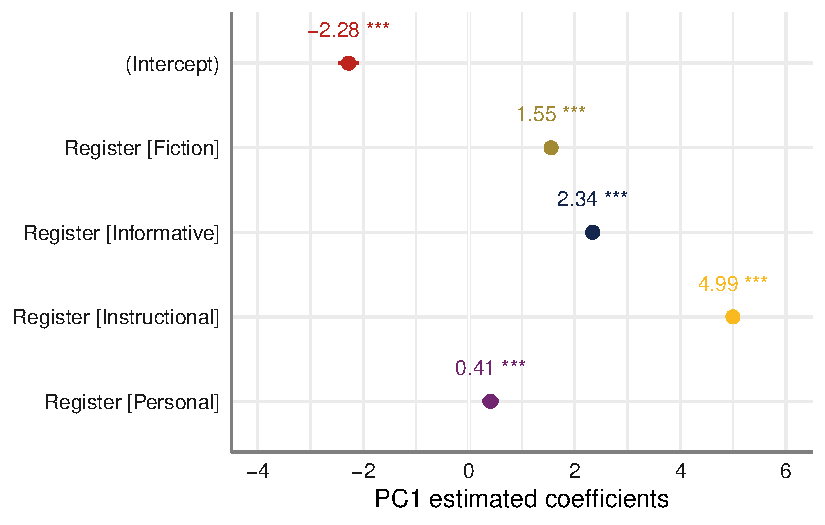
\includegraphics{E_Ch6_Analysis_files/figure-pdf/Dim1fixed-1.pdf}

\begin{Shaded}
\begin{Highlighting}[]
\CommentTok{\#ggsave(here("plots", "TxB\_PCA1\_lmer\_fixedeffects\_Register.svg"), height = 3, width = 8)}
\end{Highlighting}
\end{Shaded}

The \texttt{emmeans} and \texttt{pairs} functions are used to compare
the estimated Dim1 scores for each register and to compare these to one
another.

\begin{Shaded}
\begin{Highlighting}[]
\NormalTok{Register\_results }\OtherTok{\textless{}{-}} \FunctionTok{emmeans}\NormalTok{(md1Register, }\StringTok{"Register"}\NormalTok{)}
\FunctionTok{summary}\NormalTok{(Register\_results)}
\end{Highlighting}
\end{Shaded}

\begin{verbatim}
 Register       emmean    SE   df lower.CL upper.CL
 Conversation  -2.2793 0.102 11.6   -2.502   -2.056
 Fiction       -0.7267 0.106 13.9   -0.955   -0.498
 Informative    0.0603 0.104 12.7   -0.165    0.286
 Instructional  2.7141 0.101 11.3    2.492    2.937
 Personal      -1.8734 0.122 25.5   -2.125   -1.622

Degrees-of-freedom method: kenward-roger 
Confidence level used: 0.95 
\end{verbatim}

\begin{Shaded}
\begin{Highlighting}[]
\NormalTok{comparisons }\OtherTok{\textless{}{-}} \FunctionTok{pairs}\NormalTok{(Register\_results, }\AttributeTok{adjust =} \StringTok{"tukey"}\NormalTok{)}
\NormalTok{comparisons}
\end{Highlighting}
\end{Shaded}

\begin{verbatim}
 contrast                     estimate     SE   df  t.ratio p.value
 Conversation - Fiction         -1.553 0.0508 1963  -30.535  <.0001
 Conversation - Informative     -2.340 0.0465 1961  -50.341  <.0001
 Conversation - Instructional   -4.993 0.0399 1961 -125.141  <.0001
 Conversation - Personal        -0.406 0.0791 1958   -5.134  <.0001
 Fiction - Informative          -0.787 0.0557 1962  -14.135  <.0001
 Fiction - Instructional        -3.441 0.0497 1962  -69.168  <.0001
 Fiction - Personal              1.147 0.0840 1958   13.645  <.0001
 Informative - Instructional    -2.654 0.0447 1957  -59.399  <.0001
 Informative - Personal          1.934 0.0816 1957   23.692  <.0001
 Instructional - Personal        4.587 0.0780 1957   58.820  <.0001

Degrees-of-freedom method: kenward-roger 
P value adjustment: tukey method for comparing a family of 5 estimates 
\end{verbatim}

\begin{Shaded}
\begin{Highlighting}[]
\CommentTok{\#write\_last\_clip()}
\FunctionTok{confint}\NormalTok{(comparisons)}
\end{Highlighting}
\end{Shaded}

\begin{verbatim}
 contrast                     estimate     SE   df lower.CL upper.CL
 Conversation - Fiction         -1.553 0.0508 1963   -1.691   -1.414
 Conversation - Informative     -2.340 0.0465 1961   -2.466   -2.213
 Conversation - Instructional   -4.993 0.0399 1961   -5.102   -4.884
 Conversation - Personal        -0.406 0.0791 1958   -0.622   -0.190
 Fiction - Informative          -0.787 0.0557 1962   -0.939   -0.635
 Fiction - Instructional        -3.441 0.0497 1962   -3.577   -3.305
 Fiction - Personal              1.147 0.0840 1958    0.917    1.376
 Informative - Instructional    -2.654 0.0447 1957   -2.776   -2.532
 Informative - Personal          1.934 0.0816 1957    1.711    2.156
 Instructional - Personal        4.587 0.0780 1957    4.374    4.800

Degrees-of-freedom method: kenward-roger 
Confidence level used: 0.95 
Conf-level adjustment: tukey method for comparing a family of 5 estimates 
\end{verbatim}

\begin{Shaded}
\begin{Highlighting}[]
\CommentTok{\#write\_last\_clip()}
\end{Highlighting}
\end{Shaded}

We can also visualise the estimated coefficients for the textbook
series, which is modelled here as a random effect.

\begin{Shaded}
\begin{Highlighting}[]
\FunctionTok{plot\_model}\NormalTok{(md1, }
           \AttributeTok{type =} \StringTok{"re"}\NormalTok{, }\CommentTok{\# Option to visualise random effects}
           \AttributeTok{show.values=}\ConstantTok{TRUE}\NormalTok{, }
           \AttributeTok{show.p=}\ConstantTok{TRUE}\NormalTok{,}
           \AttributeTok{value.offset =}\NormalTok{ .}\DecValTok{4}\NormalTok{,}
           \AttributeTok{value.size =} \FloatTok{3.5}\NormalTok{,}
           \AttributeTok{colors =} \StringTok{"bw"}\NormalTok{,}
           \AttributeTok{wrap.labels =} \DecValTok{40}\NormalTok{,}
           \AttributeTok{axis.title =} \StringTok{"PC1 estimated coefficients"}\NormalTok{) }\SpecialCharTok{+}
  \FunctionTok{theme\_sjplot2}\NormalTok{()}
\end{Highlighting}
\end{Shaded}

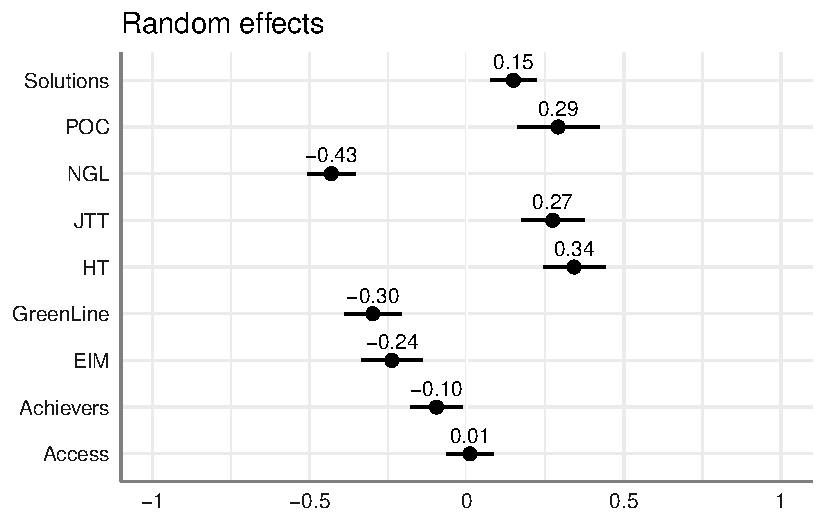
\includegraphics{E_Ch6_Analysis_files/figure-pdf/Dim1random-1.pdf}

\begin{Shaded}
\begin{Highlighting}[]
\CommentTok{\#ggsave(here("plots", "TxB\_PCA1\_lmer\_randomeffects.svg"), height = 3, width = 8)}
\end{Highlighting}
\end{Shaded}

\subsection{Dimension 2: `Involved vs.~Informational
Production'}\label{dimension-2-involved-vs.-informational-production}

\begin{Shaded}
\begin{Highlighting}[]
\NormalTok{md2 }\OtherTok{\textless{}{-}} \FunctionTok{lmer}\NormalTok{(PC2 }\SpecialCharTok{\textasciitilde{}}\NormalTok{ Register}\SpecialCharTok{*}\NormalTok{Level }\SpecialCharTok{+}\NormalTok{ (}\DecValTok{1}\SpecialCharTok{|}\NormalTok{Series), }\AttributeTok{data =}\NormalTok{ res.ind, }\AttributeTok{REML =} \ConstantTok{FALSE}\NormalTok{)}
\NormalTok{md2Register }\OtherTok{\textless{}{-}} \FunctionTok{lmer}\NormalTok{(PC2 }\SpecialCharTok{\textasciitilde{}}\NormalTok{ Register }\SpecialCharTok{+}\NormalTok{ (}\DecValTok{1}\SpecialCharTok{|}\NormalTok{Series), }\AttributeTok{data =}\NormalTok{ res.ind, }\AttributeTok{REML =} \ConstantTok{FALSE}\NormalTok{)}
\NormalTok{md2Level }\OtherTok{\textless{}{-}} \FunctionTok{lmer}\NormalTok{(PC2 }\SpecialCharTok{\textasciitilde{}}\NormalTok{ Level }\SpecialCharTok{+}\NormalTok{ (}\DecValTok{1}\SpecialCharTok{|}\NormalTok{Series), }\AttributeTok{data =}\NormalTok{ res.ind, }\AttributeTok{REML =} \ConstantTok{FALSE}\NormalTok{)}
\FunctionTok{anova}\NormalTok{(md2, md2Register, md2Level)}
\end{Highlighting}
\end{Shaded}

\begin{verbatim}
Data: res.ind
Models:
md2Register: PC2 ~ Register + (1 | Series)
md2Level: PC2 ~ Level + (1 | Series)
md2: PC2 ~ Register * Level + (1 | Series)
            npar    AIC    BIC  logLik deviance  Chisq Df Pr(>Chisq)    
md2Register    7 6155.2 6194.3 -3070.6   6141.2                         
md2Level       7 7290.1 7329.2 -3638.1   7276.1    0.0  0               
md2           27 5200.9 5351.6 -2573.4   5146.9 2129.2 20  < 2.2e-16 ***
---
Signif. codes:  0 '***' 0.001 '**' 0.01 '*' 0.05 '.' 0.1 ' ' 1
\end{verbatim}

\begin{Shaded}
\begin{Highlighting}[]
\FunctionTok{tab\_model}\NormalTok{(md2) }\CommentTok{\# Marginal R2 = 0.723}
\end{Highlighting}
\end{Shaded}

\begin{Shaded}
\begin{Highlighting}[]
\CommentTok{\# tab\_model(md2Register) \# Marginal R2 = 0.558}
\CommentTok{\# tab\_model(md2Level) \# Marginal R2 = 0.228}
\end{Highlighting}
\end{Shaded}

Estimated coefficients of fixed effects on Dim2 scores:

\begin{Shaded}
\begin{Highlighting}[]
\FunctionTok{plot\_model}\NormalTok{(md2, }
           \AttributeTok{type =} \StringTok{"est"}\NormalTok{,}
           \AttributeTok{show.intercept =} \ConstantTok{TRUE}\NormalTok{,}
           \AttributeTok{show.values=}\ConstantTok{TRUE}\NormalTok{, }
           \AttributeTok{show.p=}\ConstantTok{TRUE}\NormalTok{,}
           \AttributeTok{value.offset =}\NormalTok{ .}\DecValTok{4}\NormalTok{,}
           \AttributeTok{value.size =} \FloatTok{3.5}\NormalTok{,}
           \AttributeTok{colors =}\NormalTok{ palette[}\FunctionTok{c}\NormalTok{(}\DecValTok{1}\SpecialCharTok{:}\DecValTok{3}\NormalTok{,}\DecValTok{8}\NormalTok{,}\DecValTok{7}\NormalTok{)],}
           \AttributeTok{group.terms =} \FunctionTok{c}\NormalTok{(}\DecValTok{1}\SpecialCharTok{:}\DecValTok{5}\NormalTok{,}\DecValTok{1}\NormalTok{,}\DecValTok{1}\NormalTok{,}\DecValTok{1}\NormalTok{,}\DecValTok{1}\NormalTok{,}\DecValTok{2}\SpecialCharTok{:}\DecValTok{5}\NormalTok{,}\DecValTok{2}\SpecialCharTok{:}\DecValTok{5}\NormalTok{,}\DecValTok{2}\SpecialCharTok{:}\DecValTok{5}\NormalTok{,}\DecValTok{2}\SpecialCharTok{:}\DecValTok{5}\NormalTok{), }
           \AttributeTok{title =} \StringTok{""}\NormalTok{,}
           \AttributeTok{wrap.labels =} \DecValTok{40}\NormalTok{,}
           \AttributeTok{axis.title =} \StringTok{"PC2 estimated coefficients"}\NormalTok{) }\SpecialCharTok{+}
  \FunctionTok{theme\_sjplot2}\NormalTok{() }
\end{Highlighting}
\end{Shaded}

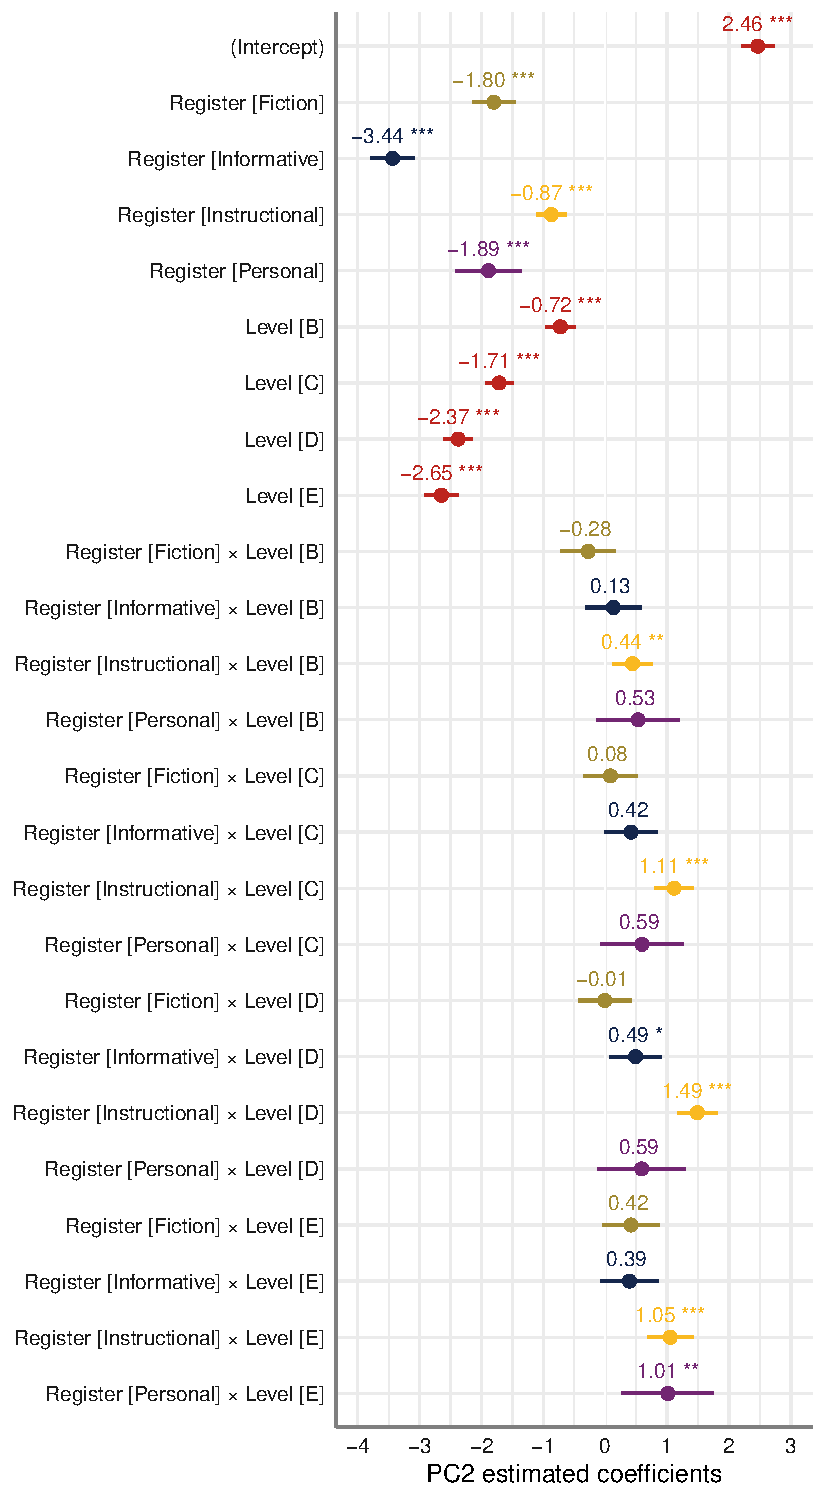
\includegraphics{E_Ch6_Analysis_files/figure-pdf/Dim2fixed-1.pdf}

\begin{Shaded}
\begin{Highlighting}[]
\CommentTok{\#ggsave(here("plots", "TxB\_PCA2\_lmer\_fixedeffects.svg"), height = 8, width = 8)}
\end{Highlighting}
\end{Shaded}

Estimated coefficients of random effects on Dim2 scores:

\begin{Shaded}
\begin{Highlighting}[]
\DocumentationTok{\#\# Random intercepts}
\FunctionTok{plot\_model}\NormalTok{(md2, }
           \AttributeTok{type =} \StringTok{"re"}\NormalTok{, }\CommentTok{\# Option to visualise random effects}
           \AttributeTok{show.values=}\ConstantTok{TRUE}\NormalTok{, }
           \AttributeTok{show.p=}\ConstantTok{TRUE}\NormalTok{,}
           \AttributeTok{value.offset =}\NormalTok{ .}\DecValTok{4}\NormalTok{,}
           \AttributeTok{value.size =} \FloatTok{3.5}\NormalTok{,}
           \AttributeTok{colors =} \StringTok{"bw"}\NormalTok{,}
           \AttributeTok{wrap.labels =} \DecValTok{40}\NormalTok{,}
           \AttributeTok{axis.title =} \StringTok{"PC2 estimated coefficients"}\NormalTok{) }\SpecialCharTok{+}
  \FunctionTok{theme\_sjplot2}\NormalTok{()}
\end{Highlighting}
\end{Shaded}

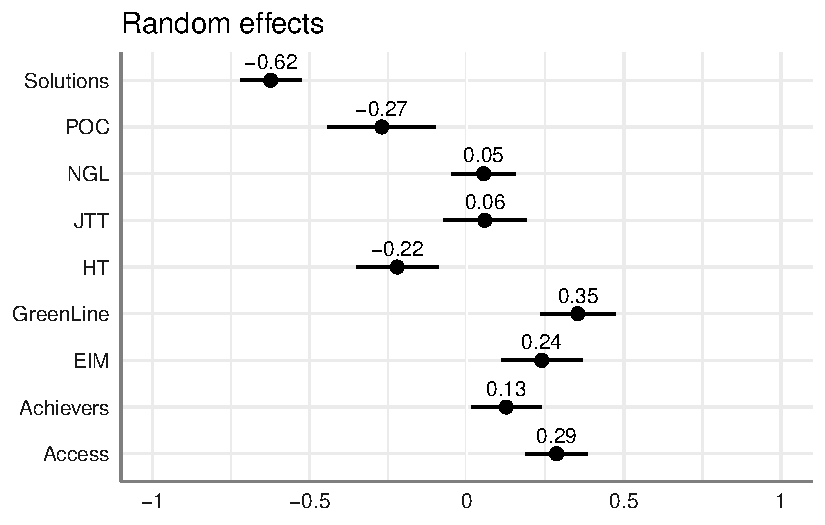
\includegraphics{E_Ch6_Analysis_files/figure-pdf/Dim2random-1.pdf}

\begin{Shaded}
\begin{Highlighting}[]
\CommentTok{\#ggsave(here("plots", "TxB\_PCA2\_lmer\_randomeffects.svg"), height = 3, width = 8)}

\CommentTok{\# Textbook Country as a random effect variable}
\NormalTok{md2country }\OtherTok{\textless{}{-}} \FunctionTok{lmer}\NormalTok{(PC2 }\SpecialCharTok{\textasciitilde{}}\NormalTok{ Register}\SpecialCharTok{*}\NormalTok{Level }\SpecialCharTok{+}\NormalTok{ (}\DecValTok{1}\SpecialCharTok{|}\NormalTok{Country), }\AttributeTok{data =}\NormalTok{ res.ind, }\AttributeTok{REML =} \ConstantTok{FALSE}\NormalTok{)}

\FunctionTok{plot\_model}\NormalTok{(md2country, }
           \AttributeTok{type =} \StringTok{"re"}\NormalTok{, }\CommentTok{\# Option to visualise random effects}
           \AttributeTok{show.values=}\ConstantTok{TRUE}\NormalTok{, }
           \AttributeTok{show.p=}\ConstantTok{TRUE}\NormalTok{,}
           \AttributeTok{value.offset =}\NormalTok{ .}\DecValTok{4}\NormalTok{,}
           \AttributeTok{value.size =} \FloatTok{3.5}\NormalTok{,}
           \AttributeTok{colors =} \StringTok{"bw"}\NormalTok{,}
           \AttributeTok{wrap.labels =} \DecValTok{40}\NormalTok{,}
           \AttributeTok{axis.title =} \StringTok{"PC2 estimated coefficients"}\NormalTok{) }\SpecialCharTok{+}
  \FunctionTok{theme\_sjplot2}\NormalTok{()}
\end{Highlighting}
\end{Shaded}

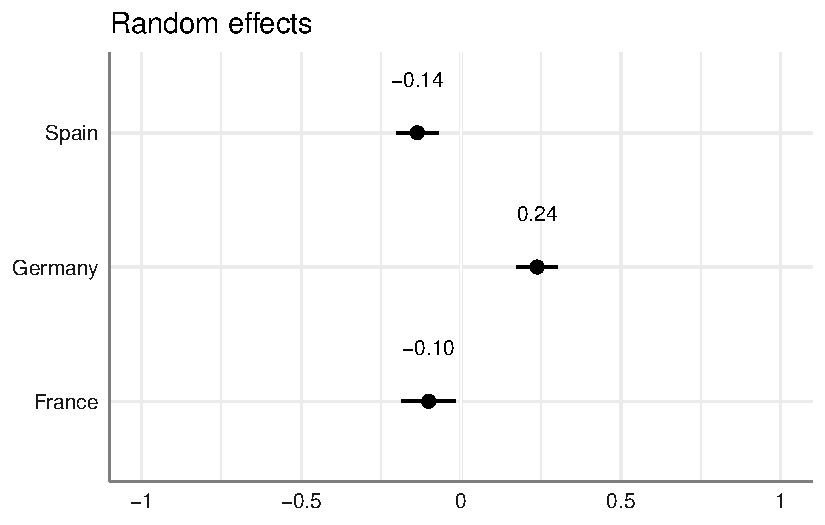
\includegraphics{E_Ch6_Analysis_files/figure-pdf/Dim2random-2.pdf}

\begin{Shaded}
\begin{Highlighting}[]
\CommentTok{\#ggsave(here("plots", "TxB\_PCA2\_lmer\_randomeffects\_country.svg"), height = 3, width = 8)}
\end{Highlighting}
\end{Shaded}

The \texttt{visreg} function is used to visualise the distributions of
the modelled Dim2 scores:

\begin{Shaded}
\begin{Highlighting}[]
\CommentTok{\# svg(here("plots", "TxB\_predicted\_PC2\_scores\_interactions.svg"), height = 5, width = 8)}
\FunctionTok{visreg}\NormalTok{(md2, }\AttributeTok{xvar =} \StringTok{"Level"}\NormalTok{, }\AttributeTok{by=}\StringTok{"Register"}\NormalTok{, }\AttributeTok{type =} \StringTok{"conditional"}\NormalTok{,}
       \AttributeTok{line=}\FunctionTok{list}\NormalTok{(}\AttributeTok{col=}\StringTok{"darkred"}\NormalTok{), }
       \AttributeTok{xlab =} \StringTok{"Textbook Level"}\NormalTok{, }\AttributeTok{ylab =} \StringTok{"PC2"}
       \CommentTok{\#,gg = TRUE}
\NormalTok{       ,}\AttributeTok{layout=}\FunctionTok{c}\NormalTok{(}\DecValTok{5}\NormalTok{,}\DecValTok{1}\NormalTok{)}
\NormalTok{)}
\end{Highlighting}
\end{Shaded}

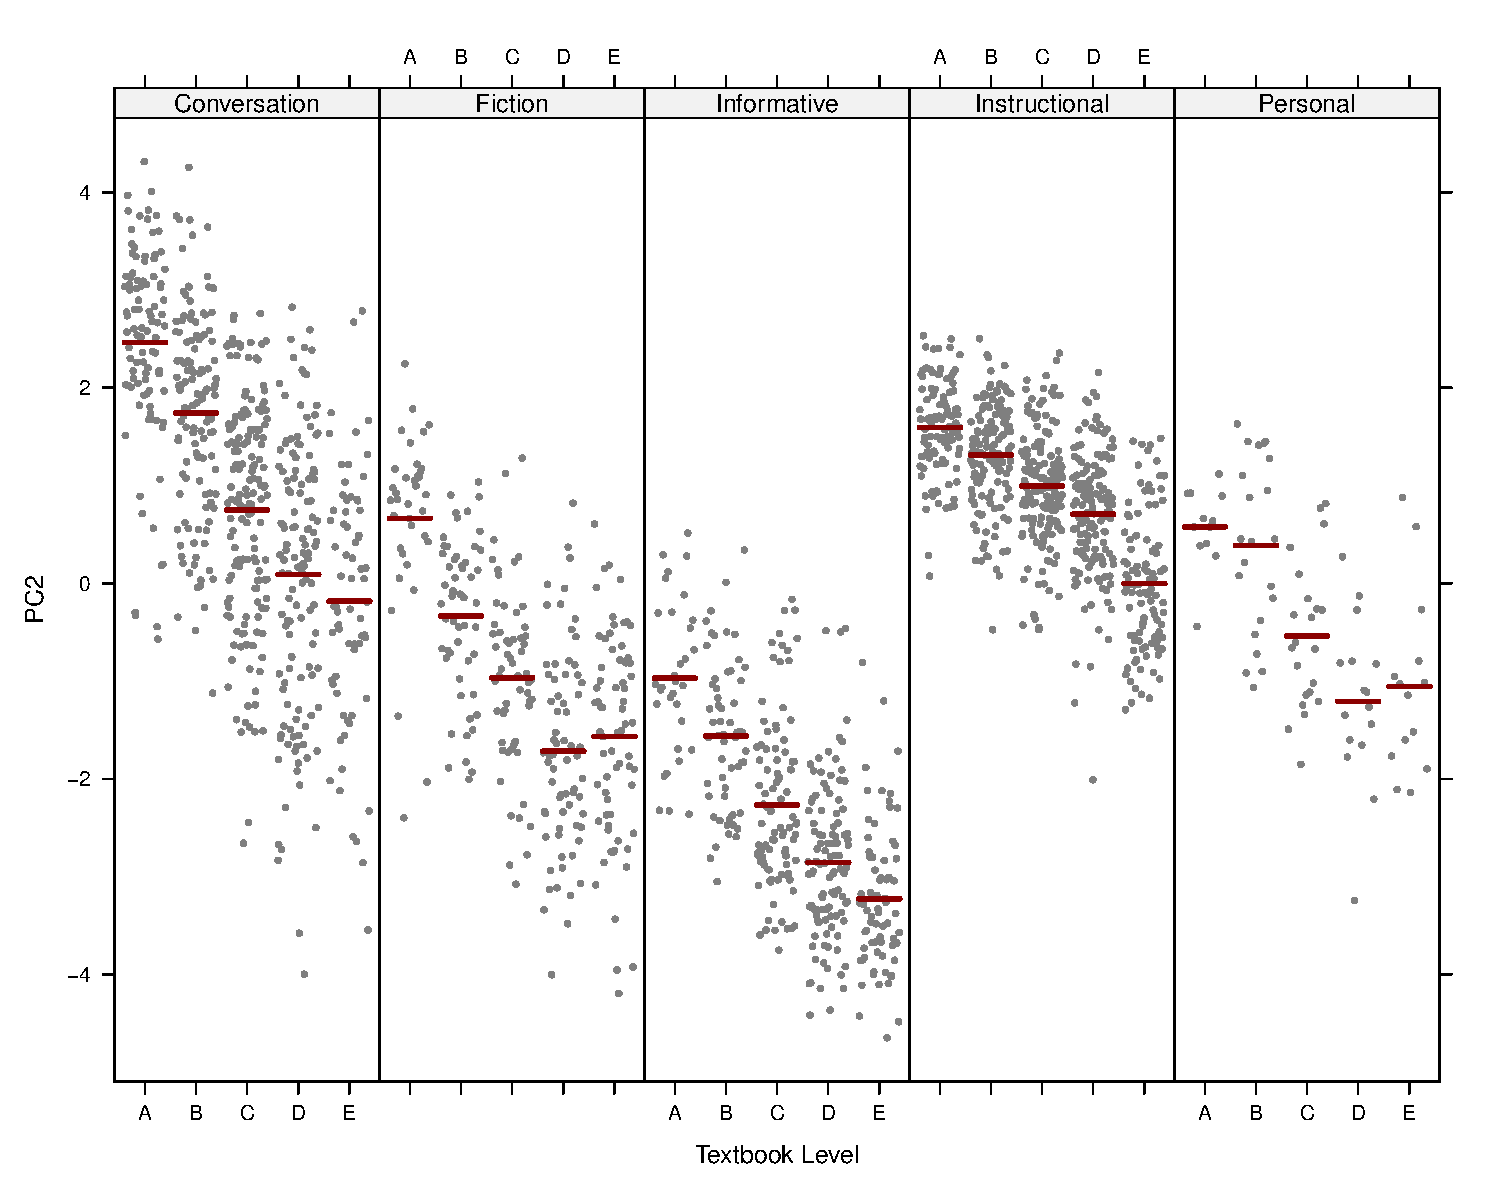
\includegraphics{E_Ch6_Analysis_files/figure-pdf/Dim2estimateplots-1.pdf}

\begin{Shaded}
\begin{Highlighting}[]
\CommentTok{\# dev.off()}

\CommentTok{\# Textbook Series{-}Register interactions}
\NormalTok{visreg}\SpecialCharTok{::}\FunctionTok{visreg}\NormalTok{(md2, }\StringTok{"Register"}\NormalTok{, }\AttributeTok{by=}\StringTok{"Series"}\NormalTok{, }\AttributeTok{re.form=}\SpecialCharTok{\textasciitilde{}}\NormalTok{(}\DecValTok{1}\SpecialCharTok{|}\NormalTok{Series),}
               \AttributeTok{ylab=}\StringTok{"PC2"}\NormalTok{, }\AttributeTok{line=}\FunctionTok{list}\NormalTok{(}\AttributeTok{col=}\StringTok{"darkred"}\NormalTok{))}
\end{Highlighting}
\end{Shaded}

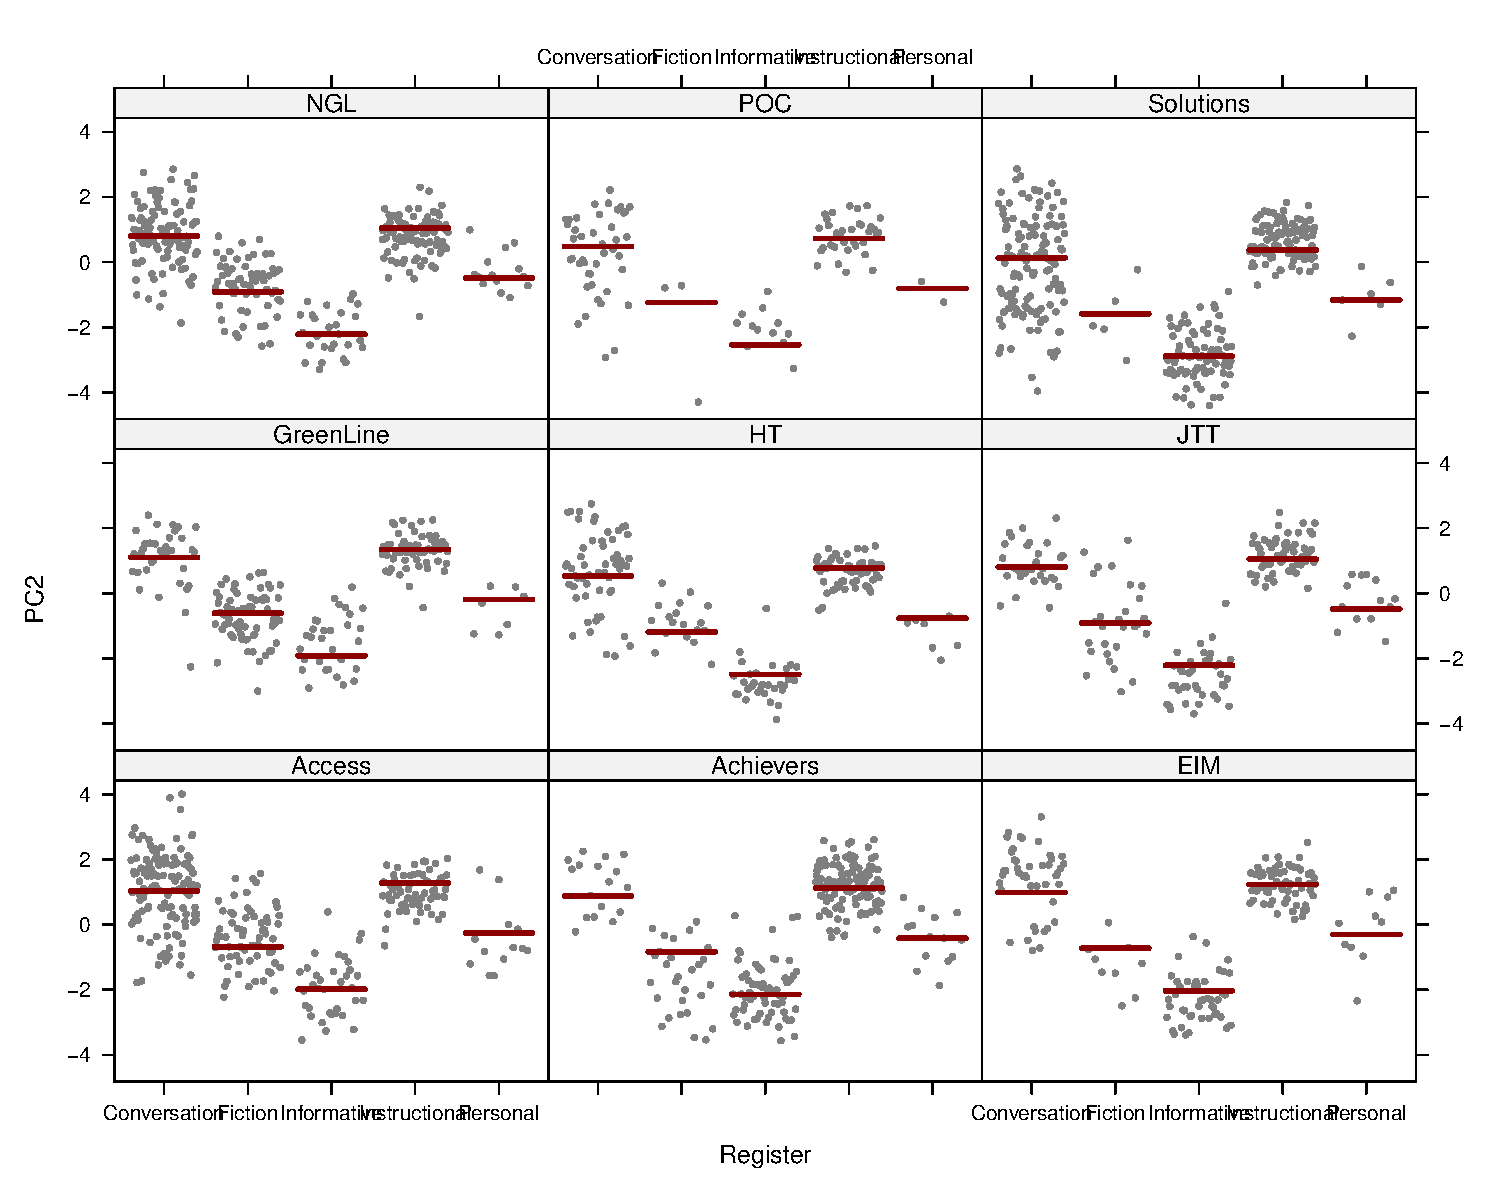
\includegraphics{E_Ch6_Analysis_files/figure-pdf/Dim2estimateplots-2.pdf}

\begin{Shaded}
\begin{Highlighting}[]
\FunctionTok{visreg}\NormalTok{(md2, }\AttributeTok{xvar =} \StringTok{"Series"}\NormalTok{, }\AttributeTok{by=}\StringTok{"Level"}\NormalTok{, }\AttributeTok{type =} \StringTok{"conditional"}\NormalTok{, }\AttributeTok{re.form=}\SpecialCharTok{\textasciitilde{}}\NormalTok{(}\DecValTok{1}\SpecialCharTok{|}\NormalTok{Series), }
       \AttributeTok{line=}\FunctionTok{list}\NormalTok{(}\AttributeTok{col=}\StringTok{"darkred"}\NormalTok{), }\AttributeTok{xlab =} \StringTok{"Textbook Series"}\NormalTok{, }\AttributeTok{ylab =} \StringTok{"PC2"}\NormalTok{,}
       \AttributeTok{layout=}\FunctionTok{c}\NormalTok{(}\DecValTok{1}\NormalTok{,}\DecValTok{5}\NormalTok{))}
\end{Highlighting}
\end{Shaded}

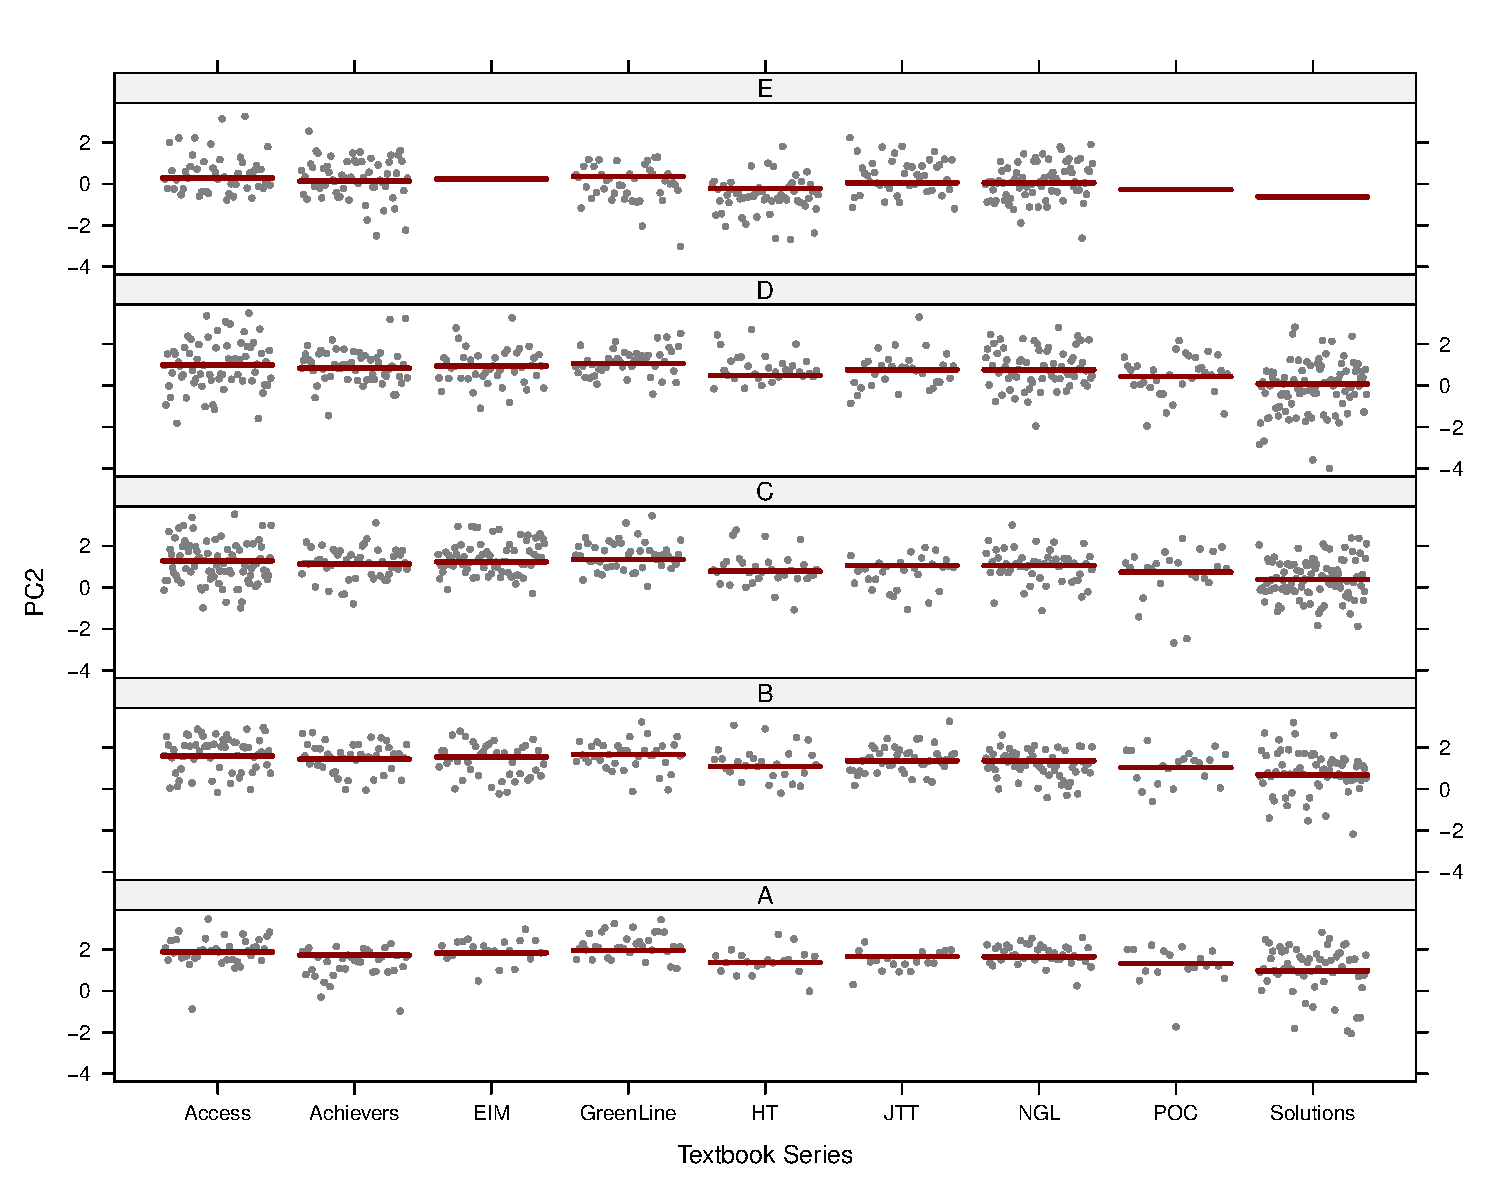
\includegraphics{E_Ch6_Analysis_files/figure-pdf/Dim2estimateplots-3.pdf}

\begin{Shaded}
\begin{Highlighting}[]
\CommentTok{\# Textbook Series{-}Register interactions}
\CommentTok{\# svg(here("plots", "TxB\_PCA2\_lmer\_randomeffects\_country\_register.svg"), height = 5, width = 8)}
\NormalTok{visreg}\SpecialCharTok{::}\FunctionTok{visreg}\NormalTok{(md2country, }\StringTok{"Country"}\NormalTok{, }\AttributeTok{by=}\StringTok{"Register"}\NormalTok{, }\AttributeTok{re.form=}\SpecialCharTok{\textasciitilde{}}\NormalTok{(}\DecValTok{1}\SpecialCharTok{|}\NormalTok{Country),}
               \AttributeTok{ylab=}\StringTok{"PC2"}\NormalTok{, }\AttributeTok{line=}\FunctionTok{list}\NormalTok{(}\AttributeTok{col=}\StringTok{"darkred"}\NormalTok{))}
\end{Highlighting}
\end{Shaded}

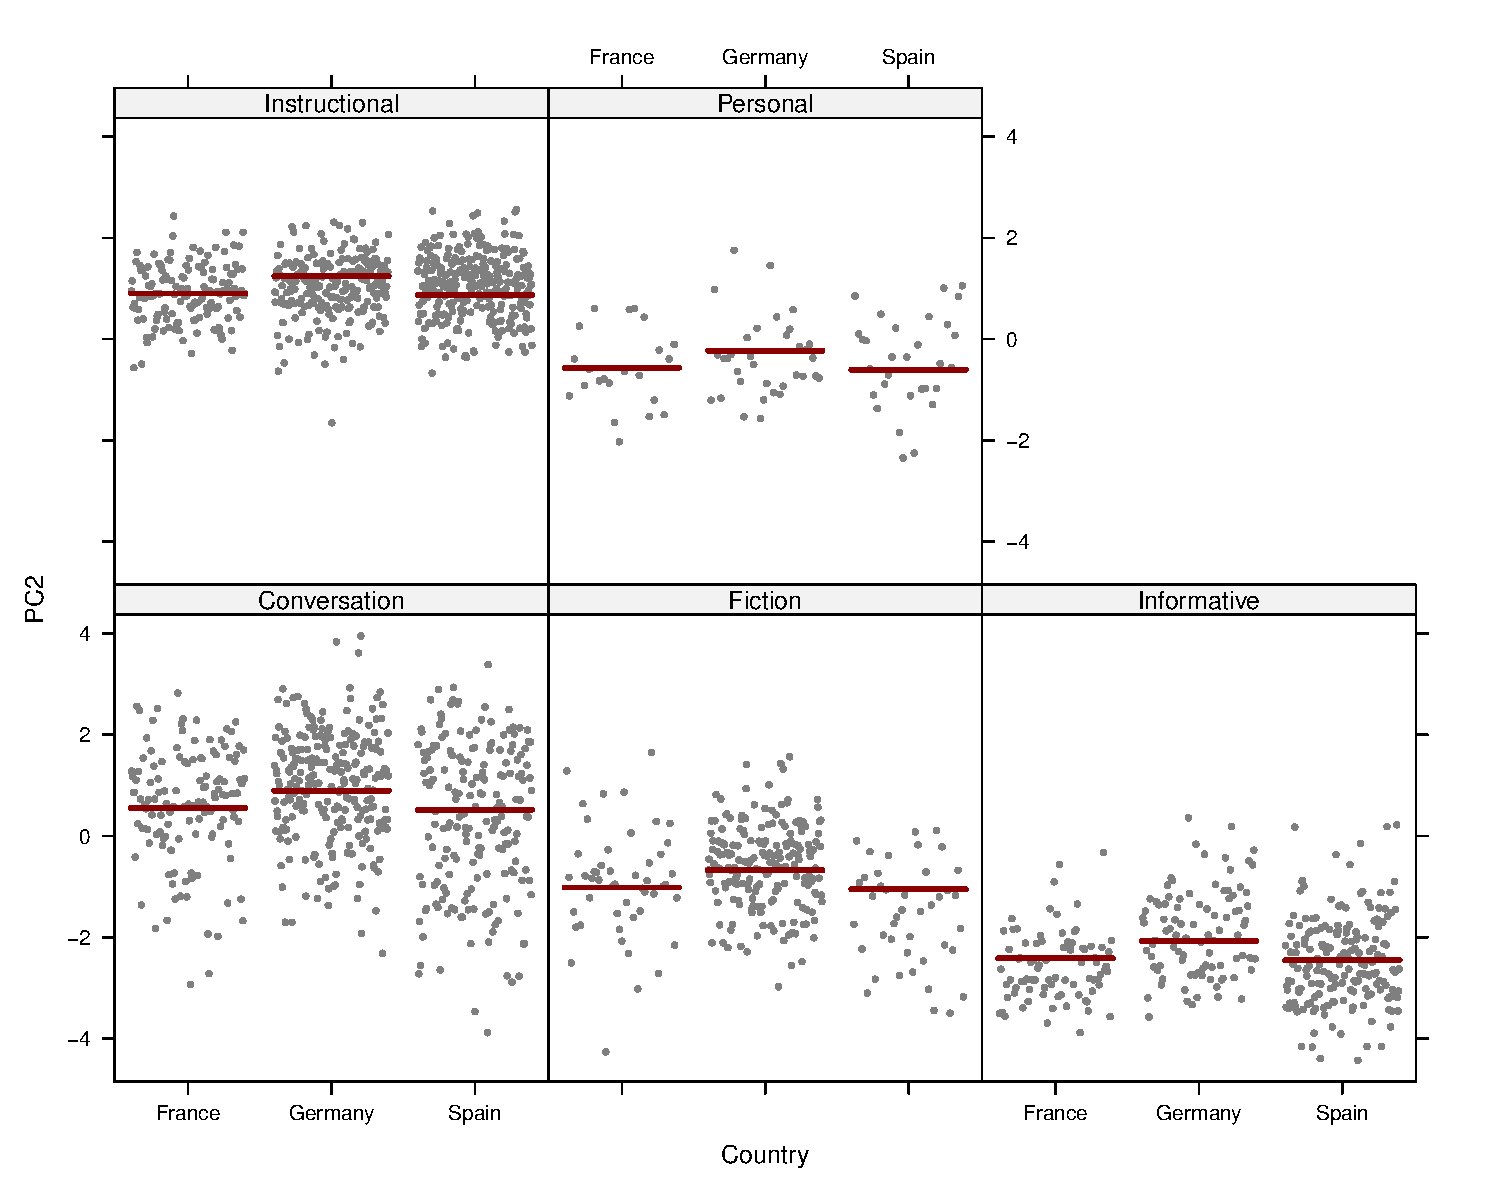
\includegraphics{E_Ch6_Analysis_files/figure-pdf/Dim2estimateplots-4.pdf}

\begin{Shaded}
\begin{Highlighting}[]
\CommentTok{\# dev.off()}
\end{Highlighting}
\end{Shaded}

\subsection{Dimension 3: `Narrative vs.~factual
discourse'}\label{dimension-3-narrative-vs.-factual-discourse}

\begin{Shaded}
\begin{Highlighting}[]
\NormalTok{md3 }\OtherTok{\textless{}{-}} \FunctionTok{lmer}\NormalTok{(PC3 }\SpecialCharTok{\textasciitilde{}}\NormalTok{ Register}\SpecialCharTok{*}\NormalTok{Level }\SpecialCharTok{+}\NormalTok{ (}\DecValTok{1}\SpecialCharTok{|}\NormalTok{Series), }\AttributeTok{data =}\NormalTok{ res.ind, }\AttributeTok{REML =} \ConstantTok{FALSE}\NormalTok{)}
\NormalTok{md3Register }\OtherTok{\textless{}{-}} \FunctionTok{lmer}\NormalTok{(PC3 }\SpecialCharTok{\textasciitilde{}}\NormalTok{ Register }\SpecialCharTok{+}\NormalTok{ (}\DecValTok{1}\SpecialCharTok{|}\NormalTok{Series), }\AttributeTok{data =}\NormalTok{ res.ind, }\AttributeTok{REML =} \ConstantTok{FALSE}\NormalTok{)}
\NormalTok{md3Level }\OtherTok{\textless{}{-}} \FunctionTok{lmer}\NormalTok{(PC3 }\SpecialCharTok{\textasciitilde{}}\NormalTok{ Level }\SpecialCharTok{+}\NormalTok{ (}\DecValTok{1}\SpecialCharTok{|}\NormalTok{Series), }\AttributeTok{data =}\NormalTok{ res.ind, }\AttributeTok{REML =} \ConstantTok{FALSE}\NormalTok{)}

\FunctionTok{anova}\NormalTok{(md3, md3Register, md3Level)}
\end{Highlighting}
\end{Shaded}

\begin{verbatim}
Data: res.ind
Models:
md3Register: PC3 ~ Register + (1 | Series)
md3Level: PC3 ~ Level + (1 | Series)
md3: PC3 ~ Register * Level + (1 | Series)
            npar    AIC    BIC  logLik deviance  Chisq Df Pr(>Chisq)    
md3Register    7 5139.9 5179.0 -2563.0   5125.9                         
md3Level       7 5528.8 5567.9 -2757.4   5514.8   0.00  0               
md3           27 4582.6 4733.3 -2264.3   4528.6 986.21 20  < 2.2e-16 ***
---
Signif. codes:  0 '***' 0.001 '**' 0.01 '*' 0.05 '.' 0.1 ' ' 1
\end{verbatim}

\begin{Shaded}
\begin{Highlighting}[]
\FunctionTok{tab\_model}\NormalTok{(md3) }\CommentTok{\# Marginal R2 = 0.436}
\end{Highlighting}
\end{Shaded}

\begin{Shaded}
\begin{Highlighting}[]
\CommentTok{\# tab\_model(md3Register) \# Marginal R2 = 0.272}
\CommentTok{\# tab\_model(md3Level) \# Marginal R2 = 0.119}

\CommentTok{\# Plot of fixed effects:}
\FunctionTok{plot\_model}\NormalTok{(md3, }
           \AttributeTok{type =} \StringTok{"est"}\NormalTok{,}
           \AttributeTok{show.intercept =} \ConstantTok{TRUE}\NormalTok{,}
           \AttributeTok{show.values=}\ConstantTok{TRUE}\NormalTok{, }
           \AttributeTok{show.p=}\ConstantTok{TRUE}\NormalTok{,}
           \AttributeTok{value.offset =}\NormalTok{ .}\DecValTok{4}\NormalTok{,}
           \AttributeTok{value.size =} \FloatTok{3.5}\NormalTok{,}
           \AttributeTok{colors =}\NormalTok{ palette[}\FunctionTok{c}\NormalTok{(}\DecValTok{1}\SpecialCharTok{:}\DecValTok{3}\NormalTok{,}\DecValTok{8}\NormalTok{,}\DecValTok{7}\NormalTok{)],}
           \AttributeTok{group.terms =} \FunctionTok{c}\NormalTok{(}\DecValTok{1}\SpecialCharTok{:}\DecValTok{5}\NormalTok{,}\DecValTok{1}\NormalTok{,}\DecValTok{1}\NormalTok{,}\DecValTok{1}\NormalTok{,}\DecValTok{1}\NormalTok{,}\DecValTok{2}\SpecialCharTok{:}\DecValTok{5}\NormalTok{,}\DecValTok{2}\SpecialCharTok{:}\DecValTok{5}\NormalTok{,}\DecValTok{2}\SpecialCharTok{:}\DecValTok{5}\NormalTok{,}\DecValTok{2}\SpecialCharTok{:}\DecValTok{5}\NormalTok{), }
           \AttributeTok{title =} \StringTok{""}\NormalTok{,}
           \AttributeTok{wrap.labels =} \DecValTok{40}\NormalTok{,}
           \AttributeTok{axis.title =} \StringTok{"PC3 estimated coefficients"}\NormalTok{) }\SpecialCharTok{+}
  \FunctionTok{theme\_sjplot2}\NormalTok{() }
\end{Highlighting}
\end{Shaded}

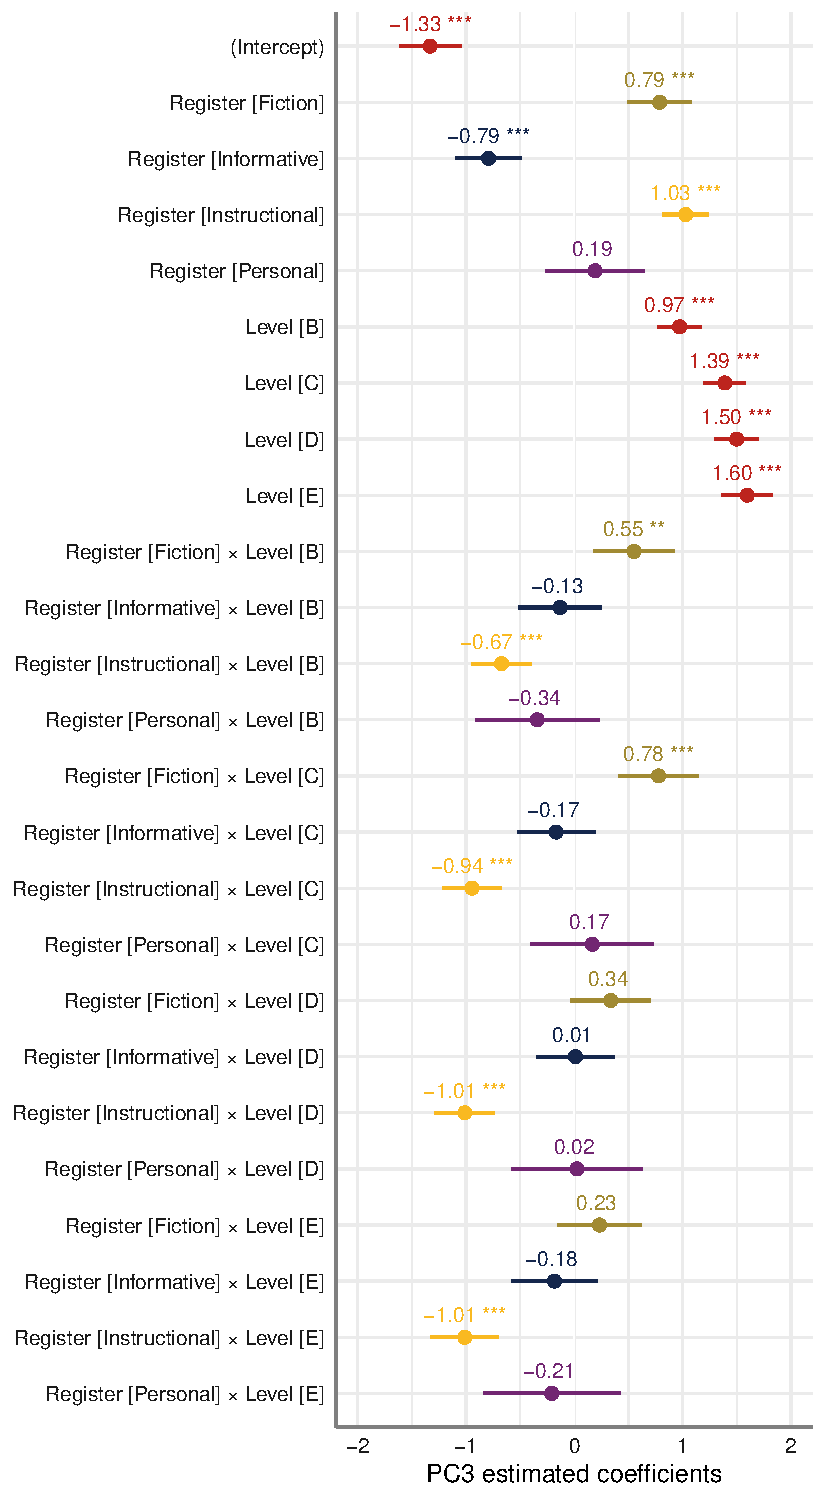
\includegraphics{E_Ch6_Analysis_files/figure-pdf/Dim3model-1.pdf}

\begin{Shaded}
\begin{Highlighting}[]
\CommentTok{\#ggsave(here("plots", "TxB\_PCA3\_lmer\_fixedeffects.svg"), height = 8, width = 8)}
\end{Highlighting}
\end{Shaded}

\begin{Shaded}
\begin{Highlighting}[]
\CommentTok{\# Plot of random effects:}
\FunctionTok{plot\_model}\NormalTok{(md3, }
           \AttributeTok{type =} \StringTok{"re"}\NormalTok{, }\CommentTok{\# Option to visualise random effects}
           \AttributeTok{show.values=}\ConstantTok{TRUE}\NormalTok{, }
           \AttributeTok{show.p=}\ConstantTok{TRUE}\NormalTok{,}
           \AttributeTok{value.offset =}\NormalTok{ .}\DecValTok{4}\NormalTok{,}
           \AttributeTok{value.size =} \FloatTok{3.5}\NormalTok{,}
           \AttributeTok{color =} \StringTok{"bw"}\NormalTok{,}
           \AttributeTok{wrap.labels =} \DecValTok{40}\NormalTok{,}
           \AttributeTok{axis.title =} \StringTok{"PC3 estimated coefficients"}\NormalTok{) }\SpecialCharTok{+}
  \FunctionTok{theme\_sjplot2}\NormalTok{()}
\end{Highlighting}
\end{Shaded}

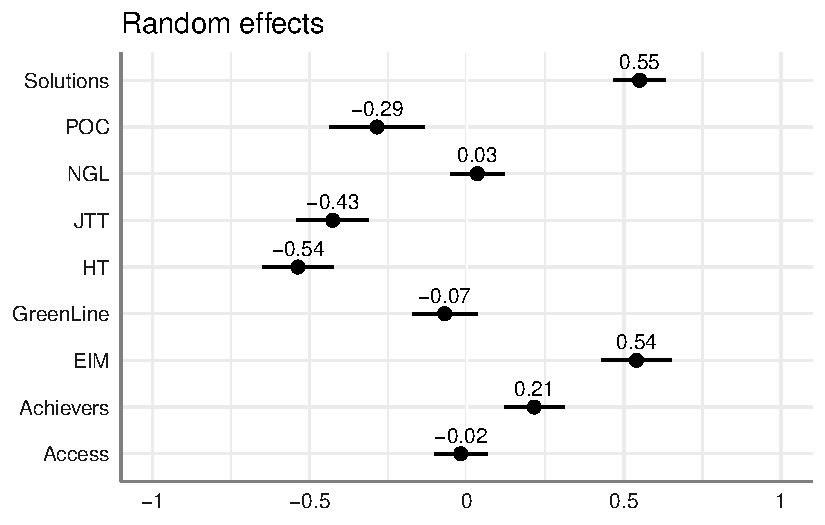
\includegraphics{E_Ch6_Analysis_files/figure-pdf/unnamed-chunk-28-1.pdf}

\begin{Shaded}
\begin{Highlighting}[]
\CommentTok{\#ggsave(here("plots", "TxB\_PCA3\_lmer\_randomeffects.svg"), height = 3, width = 8)}
\end{Highlighting}
\end{Shaded}

\begin{Shaded}
\begin{Highlighting}[]
\CommentTok{\# svg(here("plots", "TxB\_predicted\_PC3\_scores\_interactions.svg"), height = 5, width = 8)}
\FunctionTok{visreg}\NormalTok{(md3, }\AttributeTok{xvar =} \StringTok{"Level"}\NormalTok{, }\AttributeTok{by=}\StringTok{"Register"}\NormalTok{, }\AttributeTok{type =} \StringTok{"conditional"}\NormalTok{,}
       \AttributeTok{line=}\FunctionTok{list}\NormalTok{(}\AttributeTok{col=}\StringTok{"darkred"}\NormalTok{), }
       \AttributeTok{xlab =} \StringTok{"Textbook Level"}\NormalTok{, }\AttributeTok{ylab =} \StringTok{"PC3"}
       \CommentTok{\#,gg = TRUE}
\NormalTok{       ,}\AttributeTok{layout=}\FunctionTok{c}\NormalTok{(}\DecValTok{5}\NormalTok{,}\DecValTok{1}\NormalTok{)}
\NormalTok{)}
\end{Highlighting}
\end{Shaded}

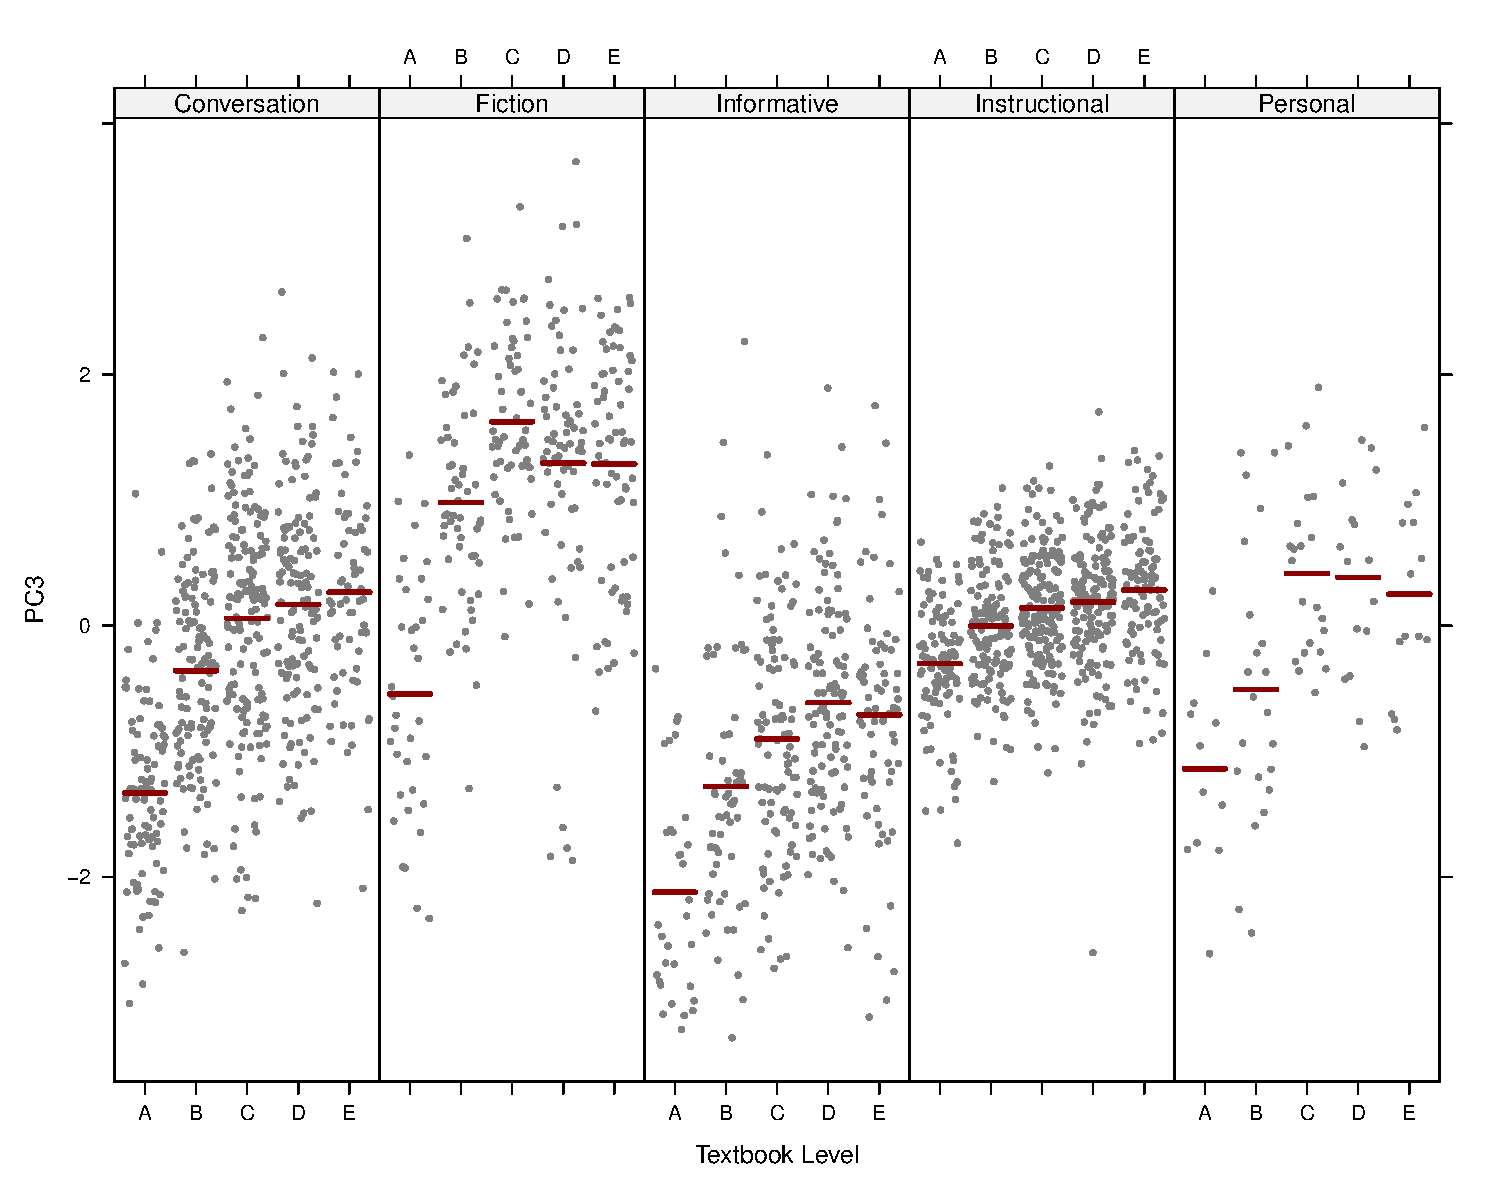
\includegraphics{E_Ch6_Analysis_files/figure-pdf/Dim3comparisons-1.pdf}

\begin{Shaded}
\begin{Highlighting}[]
\CommentTok{\# dev.off()}

\CommentTok{\# Textbook Series{-}Register interactions}
\NormalTok{visreg}\SpecialCharTok{::}\FunctionTok{visreg}\NormalTok{(md3, }\StringTok{"Series"}\NormalTok{, }\AttributeTok{by=}\StringTok{"Register"}\NormalTok{, }\AttributeTok{re.form=}\SpecialCharTok{\textasciitilde{}}\NormalTok{(}\DecValTok{1}\SpecialCharTok{|}\NormalTok{Series),}
               \AttributeTok{ylab=}\StringTok{"PC3"}\NormalTok{, }\AttributeTok{line=}\FunctionTok{list}\NormalTok{(}\AttributeTok{col=}\StringTok{"darkred"}\NormalTok{))}
\end{Highlighting}
\end{Shaded}

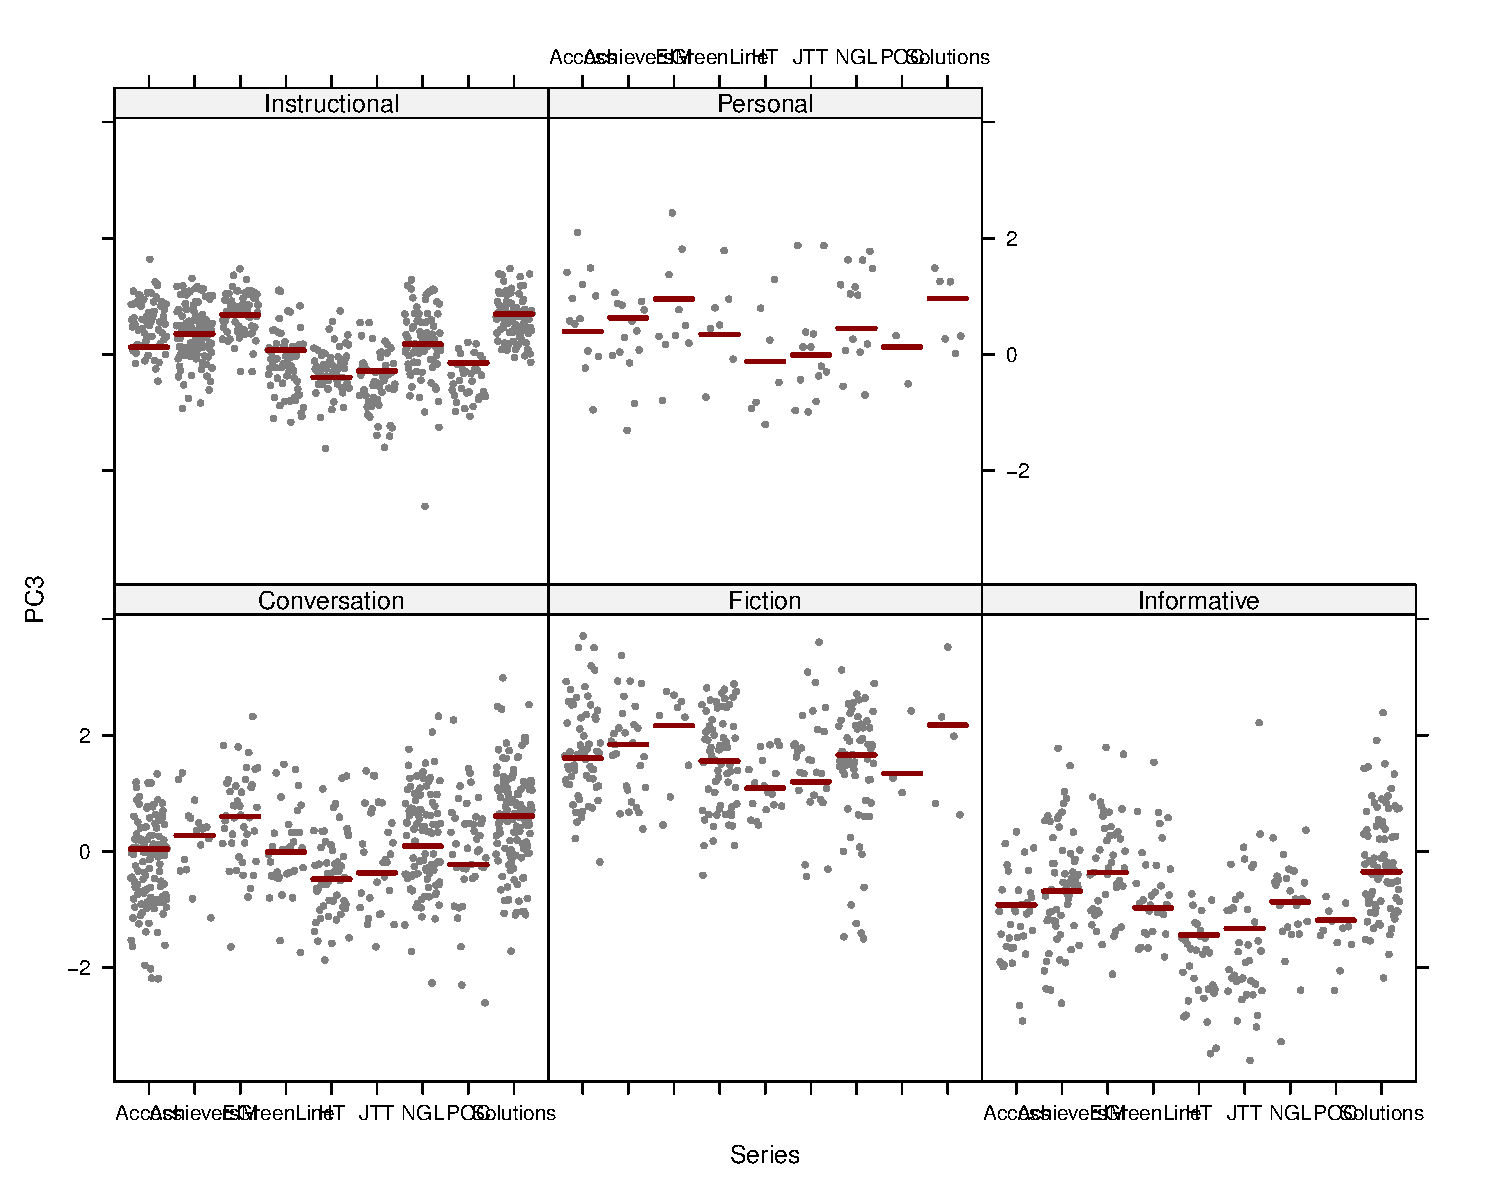
\includegraphics{E_Ch6_Analysis_files/figure-pdf/Dim3comparisons-2.pdf}

\begin{Shaded}
\begin{Highlighting}[]
\FunctionTok{visreg}\NormalTok{(md3, }\AttributeTok{xvar =} \StringTok{"Level"}\NormalTok{, }\AttributeTok{by=}\StringTok{"Series"}\NormalTok{, }\AttributeTok{type =} \StringTok{"conditional"}\NormalTok{, }\AttributeTok{re.form=}\SpecialCharTok{\textasciitilde{}}\NormalTok{(}\DecValTok{1}\SpecialCharTok{|}\NormalTok{Series), }
       \AttributeTok{line=}\FunctionTok{list}\NormalTok{(}\AttributeTok{col=}\StringTok{"darkred"}\NormalTok{), }\AttributeTok{xlab =} \StringTok{"Textbook Series"}\NormalTok{, }\AttributeTok{ylab =} \StringTok{"PC3"}\NormalTok{)}
\end{Highlighting}
\end{Shaded}

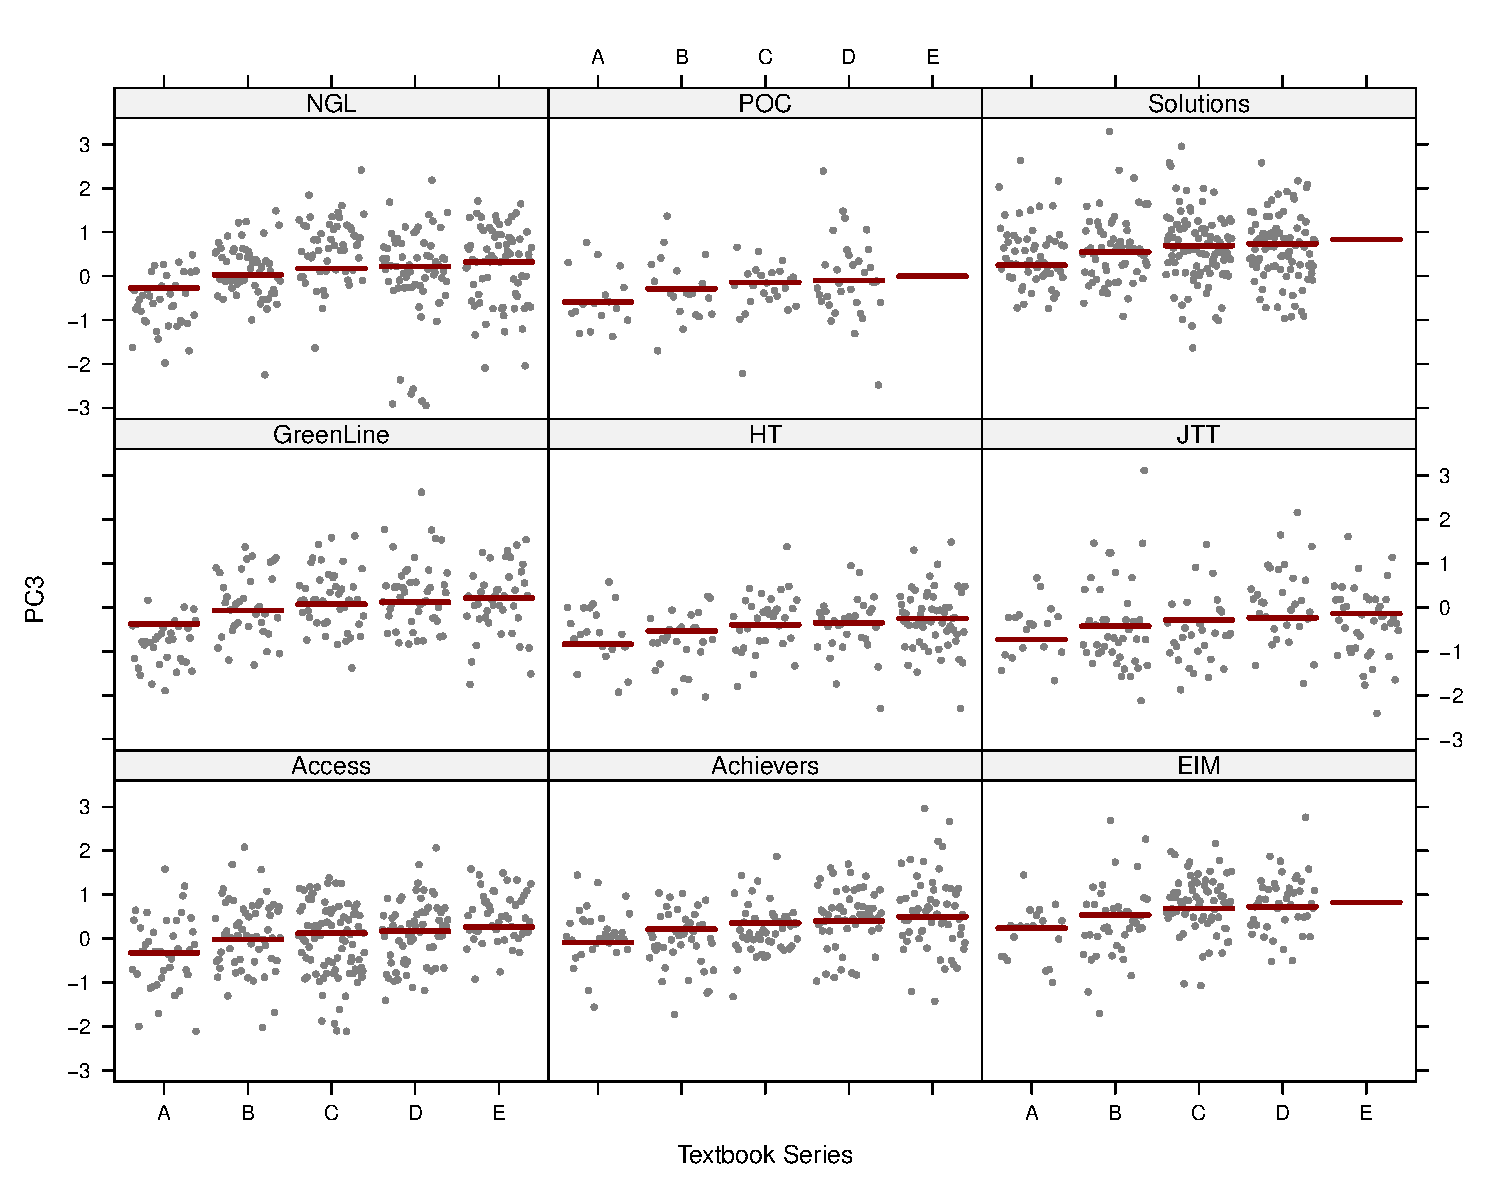
\includegraphics{E_Ch6_Analysis_files/figure-pdf/Dim3comparisons-3.pdf}

\subsection{Dimension 4: `Informational compression
vs.~elaboration'}\label{dimension-4-informational-compression-vs.-elaboration}

\begin{Shaded}
\begin{Highlighting}[]
\NormalTok{md4 }\OtherTok{\textless{}{-}} \FunctionTok{lmer}\NormalTok{(PC4 }\SpecialCharTok{\textasciitilde{}}\NormalTok{ Register}\SpecialCharTok{*}\NormalTok{Level }\SpecialCharTok{+}\NormalTok{ (}\DecValTok{1}\SpecialCharTok{|}\NormalTok{Series), }\AttributeTok{data =}\NormalTok{ res.ind, }\AttributeTok{REML =} \ConstantTok{FALSE}\NormalTok{)}
\NormalTok{md4Register }\OtherTok{\textless{}{-}} \FunctionTok{lmer}\NormalTok{(PC4 }\SpecialCharTok{\textasciitilde{}}\NormalTok{ Register }\SpecialCharTok{+}\NormalTok{ (}\DecValTok{1}\SpecialCharTok{|}\NormalTok{Series), }\AttributeTok{data =}\NormalTok{ res.ind, }\AttributeTok{REML =} \ConstantTok{FALSE}\NormalTok{)}
\NormalTok{md4Level }\OtherTok{\textless{}{-}} \FunctionTok{lmer}\NormalTok{(PC4 }\SpecialCharTok{\textasciitilde{}}\NormalTok{ Level }\SpecialCharTok{+}\NormalTok{ (}\DecValTok{1}\SpecialCharTok{|}\NormalTok{Series), }\AttributeTok{data =}\NormalTok{ res.ind, }\AttributeTok{REML =} \ConstantTok{FALSE}\NormalTok{)}

\FunctionTok{anova}\NormalTok{(md4, md4Register, md4Level)}
\end{Highlighting}
\end{Shaded}

\begin{verbatim}
Data: res.ind
Models:
md4Register: PC4 ~ Register + (1 | Series)
md4Level: PC4 ~ Level + (1 | Series)
md4: PC4 ~ Register * Level + (1 | Series)
            npar    AIC    BIC  logLik deviance  Chisq Df Pr(>Chisq)    
md4Register    7 5034.0 5073.0 -2510.0   5020.0                         
md4Level       7 5043.6 5082.7 -2514.8   5029.6   0.00  0               
md4           27 4372.1 4522.8 -2159.1   4318.1 711.52 20  < 2.2e-16 ***
---
Signif. codes:  0 '***' 0.001 '**' 0.01 '*' 0.05 '.' 0.1 ' ' 1
\end{verbatim}

\begin{Shaded}
\begin{Highlighting}[]
\FunctionTok{tab\_model}\NormalTok{(md4) }\CommentTok{\# Marginal R2 = 0.426}
\end{Highlighting}
\end{Shaded}

\begin{Shaded}
\begin{Highlighting}[]
\CommentTok{\# tab\_model(md4Register) \# Marginal R2 = 0.203}
\CommentTok{\# tab\_model(md4Level) \# Marginal R2 = 0.187}

\CommentTok{\# Plot of fixed effects:}
\FunctionTok{plot\_model}\NormalTok{(md4, }
           \AttributeTok{type =} \StringTok{"est"}\NormalTok{,}
           \AttributeTok{show.intercept =} \ConstantTok{TRUE}\NormalTok{,}
           \AttributeTok{show.values=}\ConstantTok{TRUE}\NormalTok{, }
           \AttributeTok{show.p=}\ConstantTok{TRUE}\NormalTok{,}
           \AttributeTok{value.offset =}\NormalTok{ .}\DecValTok{4}\NormalTok{,}
           \AttributeTok{value.size =} \FloatTok{3.5}\NormalTok{,}
           \AttributeTok{colors =}\NormalTok{ palette[}\FunctionTok{c}\NormalTok{(}\DecValTok{1}\SpecialCharTok{:}\DecValTok{3}\NormalTok{,}\DecValTok{8}\NormalTok{,}\DecValTok{7}\NormalTok{)],}
           \AttributeTok{group.terms =} \FunctionTok{c}\NormalTok{(}\DecValTok{1}\SpecialCharTok{:}\DecValTok{5}\NormalTok{,}\DecValTok{1}\NormalTok{,}\DecValTok{1}\NormalTok{,}\DecValTok{1}\NormalTok{,}\DecValTok{1}\NormalTok{,}\DecValTok{2}\SpecialCharTok{:}\DecValTok{5}\NormalTok{,}\DecValTok{2}\SpecialCharTok{:}\DecValTok{5}\NormalTok{,}\DecValTok{2}\SpecialCharTok{:}\DecValTok{5}\NormalTok{,}\DecValTok{2}\SpecialCharTok{:}\DecValTok{5}\NormalTok{), }
           \AttributeTok{title =} \StringTok{""}\NormalTok{,}
           \AttributeTok{wrap.labels =} \DecValTok{40}\NormalTok{,}
           \AttributeTok{axis.title =} \StringTok{"PC4 estimated coefficients"}\NormalTok{) }\SpecialCharTok{+}
  \FunctionTok{theme\_sjplot2}\NormalTok{() }
\end{Highlighting}
\end{Shaded}

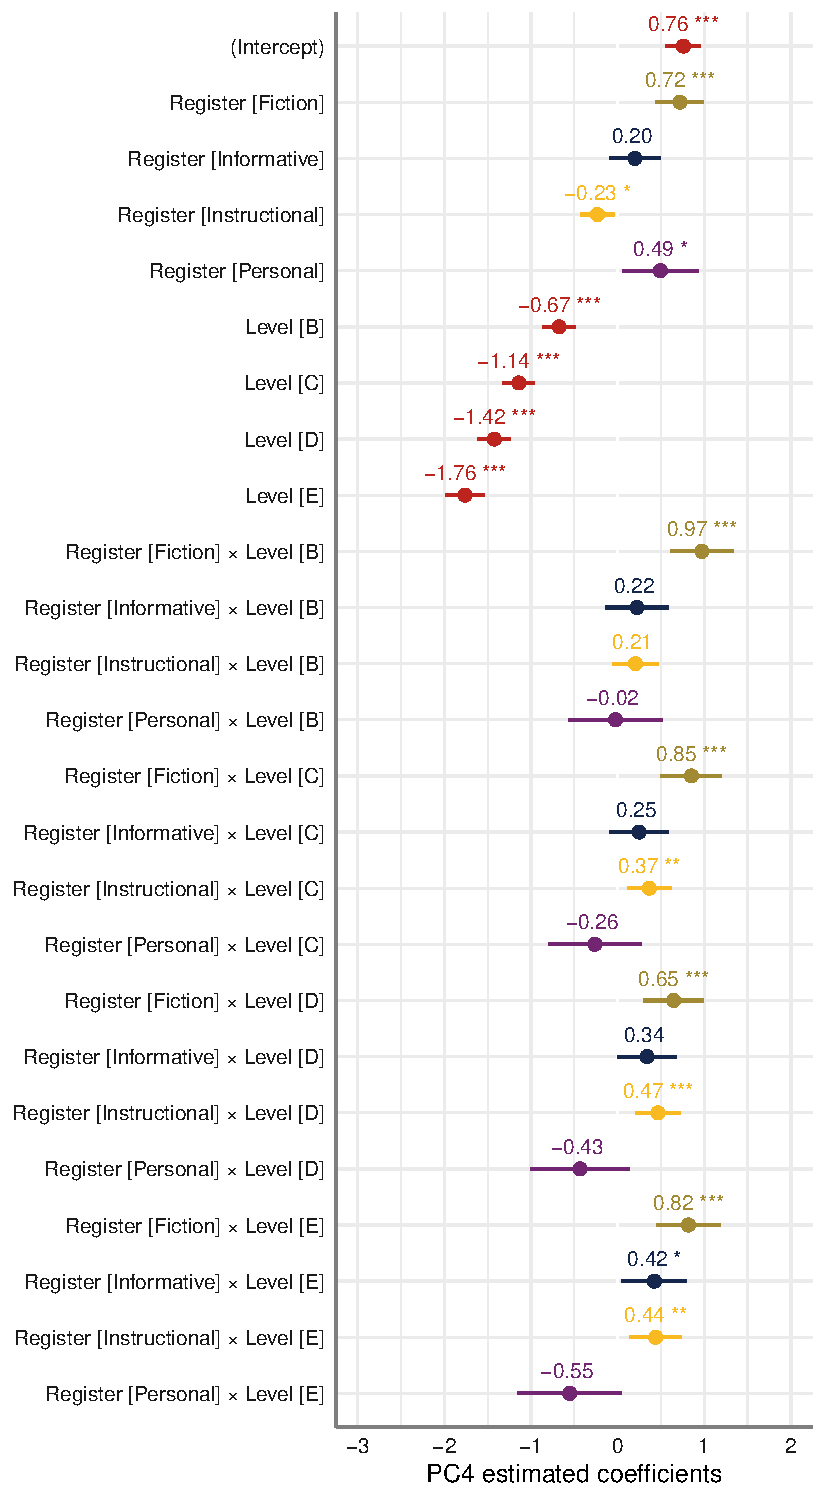
\includegraphics{E_Ch6_Analysis_files/figure-pdf/Dim4model-1.pdf}

\begin{Shaded}
\begin{Highlighting}[]
\CommentTok{\#ggsave(here("plots", "TxB\_PCA4\_lmer\_fixedeffects.svg"), height = 8, width = 8)}
\end{Highlighting}
\end{Shaded}

\begin{Shaded}
\begin{Highlighting}[]
\CommentTok{\# Plot of random effects:}
\FunctionTok{plot\_model}\NormalTok{(md4, }
           \AttributeTok{type =} \StringTok{"re"}\NormalTok{, }\CommentTok{\# Option to visualise random effects}
           \AttributeTok{show.values=}\ConstantTok{TRUE}\NormalTok{, }
           \AttributeTok{show.p=}\ConstantTok{TRUE}\NormalTok{,}
           \AttributeTok{value.offset =}\NormalTok{ .}\DecValTok{4}\NormalTok{,}
           \AttributeTok{value.size =} \FloatTok{3.5}\NormalTok{,}
           \AttributeTok{color =} \StringTok{"bw"}\NormalTok{,}
           \AttributeTok{wrap.labels =} \DecValTok{40}\NormalTok{,}
           \AttributeTok{axis.title =} \StringTok{"PC4 estimated coefficients"}\NormalTok{) }\SpecialCharTok{+}
  \FunctionTok{theme\_sjplot2}\NormalTok{()}
\end{Highlighting}
\end{Shaded}

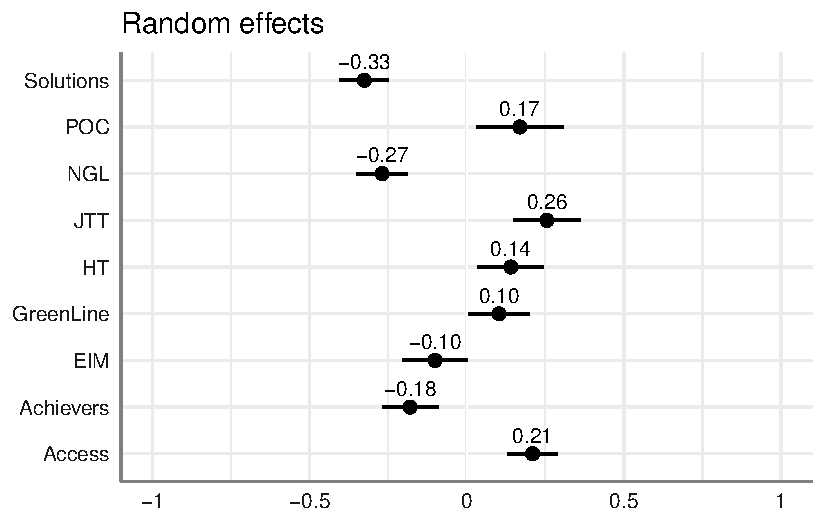
\includegraphics{E_Ch6_Analysis_files/figure-pdf/unnamed-chunk-31-1.pdf}

\begin{Shaded}
\begin{Highlighting}[]
\CommentTok{\#ggsave(here("plots", "TxB\_PCA4\_lmer\_randomeffects.svg"), height = 3, width = 8)}
\end{Highlighting}
\end{Shaded}

\begin{Shaded}
\begin{Highlighting}[]
\CommentTok{\# svg(here("plots", "TxB\_predicted\_PC4\_scores\_interactions.svg"), height = 5, width = 8)}
\FunctionTok{visreg}\NormalTok{(md4, }\AttributeTok{xvar =} \StringTok{"Level"}\NormalTok{, }\AttributeTok{by=}\StringTok{"Register"}\NormalTok{, }\AttributeTok{type =} \StringTok{"conditional"}\NormalTok{,}
       \AttributeTok{line=}\FunctionTok{list}\NormalTok{(}\AttributeTok{col=}\StringTok{"darkred"}\NormalTok{), }
       \AttributeTok{xlab =} \StringTok{"Textbook Level"}\NormalTok{, }\AttributeTok{ylab =} \StringTok{"PC4"}
       \CommentTok{\#,gg = TRUE}
\NormalTok{       ,}\AttributeTok{layout=}\FunctionTok{c}\NormalTok{(}\DecValTok{5}\NormalTok{,}\DecValTok{1}\NormalTok{)}
\NormalTok{)}
\end{Highlighting}
\end{Shaded}

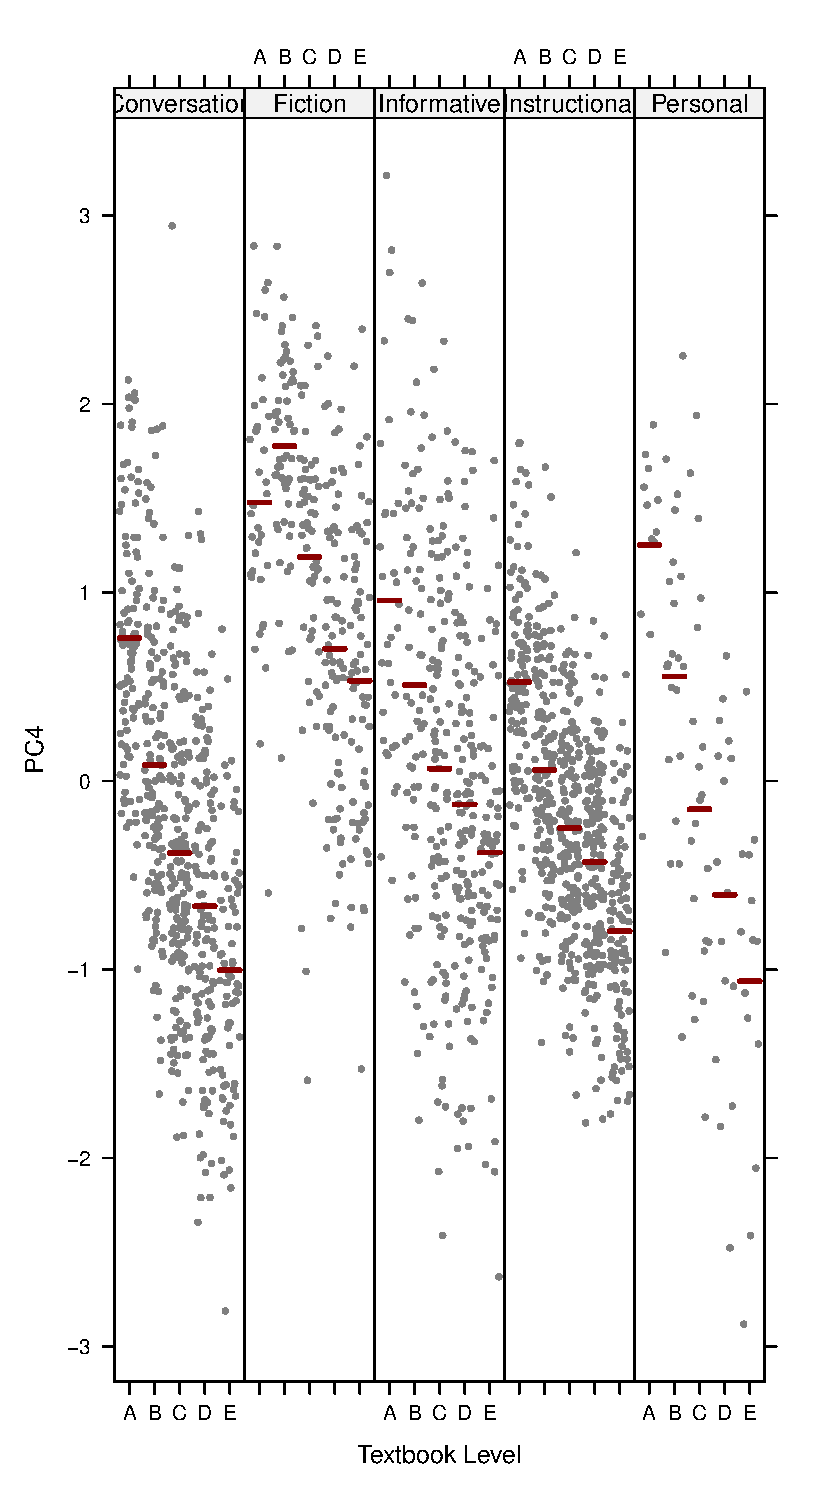
\includegraphics{E_Ch6_Analysis_files/figure-pdf/unnamed-chunk-32-1.pdf}

\begin{Shaded}
\begin{Highlighting}[]
\CommentTok{\# dev.off()}
\end{Highlighting}
\end{Shaded}

\subsection{Testing model assumptions}\label{testing-model-assumptions}

This chunk can be used to check the assumptions of all of the models
computed above. In the following example, we examine the final model
selected to predict Dim2 scores.

\begin{Shaded}
\begin{Highlighting}[]
\NormalTok{model2test }\OtherTok{\textless{}{-}}\NormalTok{ md2}

\CommentTok{\# check distribution of residuals}
\FunctionTok{plot}\NormalTok{(model2test)}
\end{Highlighting}
\end{Shaded}

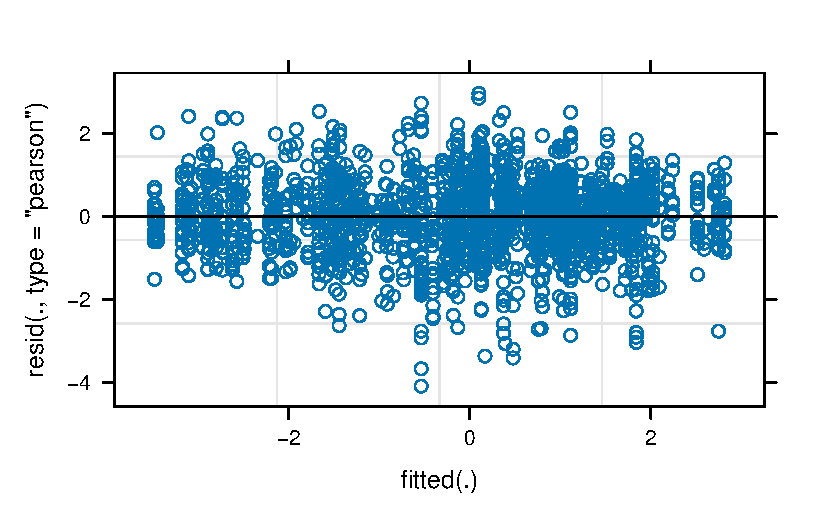
\includegraphics{E_Ch6_Analysis_files/figure-pdf/lmer-diagnostics-1.pdf}

\begin{Shaded}
\begin{Highlighting}[]
\CommentTok{\# scale{-}location plot}
\FunctionTok{plot}\NormalTok{(model2test,}
     \FunctionTok{sqrt}\NormalTok{(}\FunctionTok{abs}\NormalTok{(}\FunctionTok{resid}\NormalTok{(.)))}\SpecialCharTok{\textasciitilde{}}\FunctionTok{fitted}\NormalTok{(.),}
     \AttributeTok{type=}\FunctionTok{c}\NormalTok{(}\StringTok{"p"}\NormalTok{,}\StringTok{"smooth"}\NormalTok{), }\AttributeTok{col.line=}\DecValTok{1}\NormalTok{)}
\end{Highlighting}
\end{Shaded}

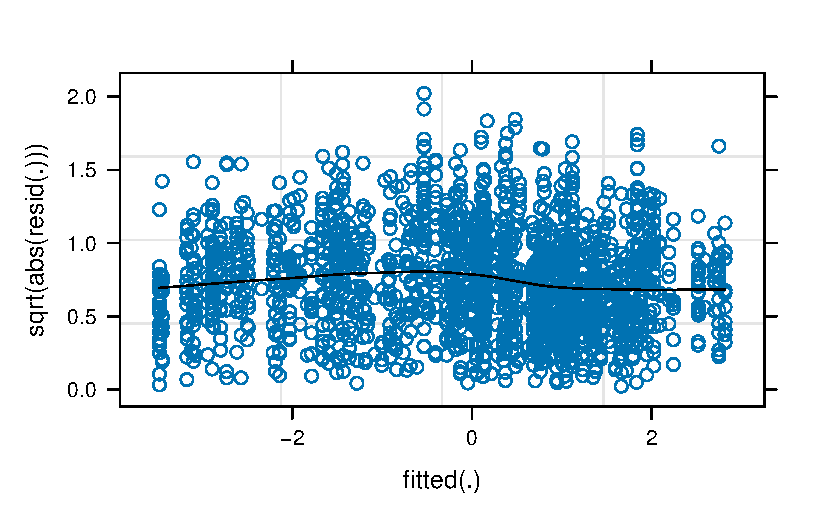
\includegraphics{E_Ch6_Analysis_files/figure-pdf/lmer-diagnostics-2.pdf}

\begin{Shaded}
\begin{Highlighting}[]
\CommentTok{\# Q{-}Q plot}
\NormalTok{lattice}\SpecialCharTok{::}\FunctionTok{qqmath}\NormalTok{(model2test)}
\end{Highlighting}
\end{Shaded}

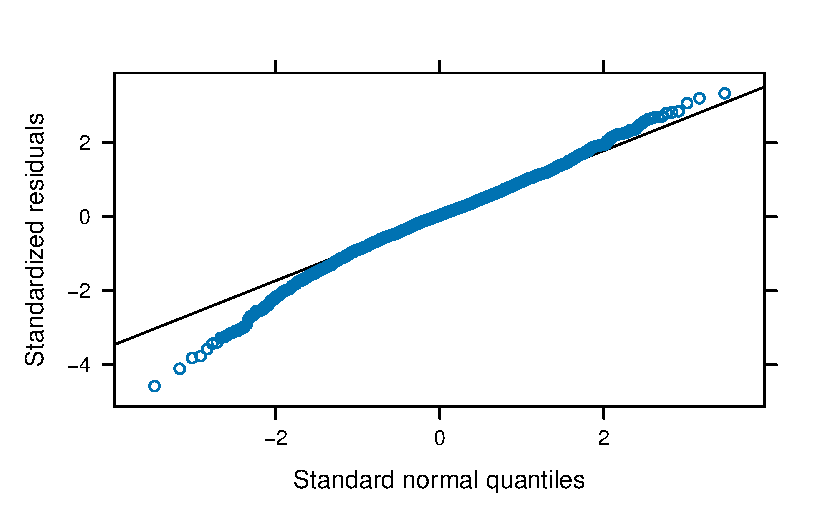
\includegraphics{E_Ch6_Analysis_files/figure-pdf/lmer-diagnostics-3.pdf}

\chapter{Data Preparation for the Model of Textbook English
vs.~`real-world'
English}\label{data-preparation-for-the-model-of-textbook-english-vs.-real-world-english}

This script documents the steps taken to pre-process the data extracted
from the Textbook English Corpus (TEC) and the three reference corpora
that were ultimately entered in the comparative multi-dimensional model
of Textbook English as compared to English outside the EFL classroom
(Chapter 7).

\section{Packages required}\label{packages-required-2}

The following packages must be installed and loaded to process the data.

\begin{Shaded}
\begin{Highlighting}[]
\CommentTok{\#renv::restore() \# Restore the project\textquotesingle{}s dependencies from the lockfile to ensure that same package versions are used as in the original thesis.}

\FunctionTok{library}\NormalTok{(broom.mixed) }\CommentTok{\# For checking singularity issues }
\FunctionTok{library}\NormalTok{(car) }\CommentTok{\# For recoding data}
\FunctionTok{library}\NormalTok{(corrplot) }\CommentTok{\# For the feature correlation matrix}
\FunctionTok{library}\NormalTok{(cowplot) }\CommentTok{\# For nice plots}
\FunctionTok{library}\NormalTok{(emmeans) }\CommentTok{\# Comparing group means of predicted values}
\FunctionTok{library}\NormalTok{(GGally) }\CommentTok{\# For ggpairs}
\FunctionTok{library}\NormalTok{(gridExtra) }\CommentTok{\# For making large faceted plots}
\FunctionTok{library}\NormalTok{(here) }\CommentTok{\# For ease of sharing}
\FunctionTok{library}\NormalTok{(knitr) }\CommentTok{\# Loaded to display the tables using the kable() function}
\FunctionTok{library}\NormalTok{(lme4) }\CommentTok{\# For mixed effects modelling}
\FunctionTok{library}\NormalTok{(psych) }\CommentTok{\# For various useful stats function, including KMO()}
\FunctionTok{library}\NormalTok{(scales) }\CommentTok{\# For working with colours}
\FunctionTok{library}\NormalTok{(sjPlot) }\CommentTok{\# For nice tabular display of regression models}
\FunctionTok{library}\NormalTok{(tidyverse) }\CommentTok{\# For data wrangling and plotting}
\FunctionTok{library}\NormalTok{(visreg) }\CommentTok{\# For nice visualisations of model results}
\NormalTok{select }\OtherTok{\textless{}{-}}\NormalTok{ dplyr}\SpecialCharTok{::}\NormalTok{select}
\NormalTok{filter }\OtherTok{\textless{}{-}}\NormalTok{ dplyr}\SpecialCharTok{::}\NormalTok{filter}
\end{Highlighting}
\end{Shaded}

\section{Data import from MFTE
outputs}\label{data-import-from-mfte-outputs}

The raw data used in this script comes from the matrices of mixed
normalised frequencies as output by the
\href{https://github.com/mshakirDr/MultiFeatureTaggerEnglish}{MFTE Perl
v. 3.1} (Le Foll 2021a).

\subsection{Spoken BNC2014}\label{spoken-bnc2014-1}

\begin{Shaded}
\begin{Highlighting}[]
\NormalTok{SpokenBNC2014 }\OtherTok{\textless{}{-}} \FunctionTok{read.delim}\NormalTok{(}\FunctionTok{here}\NormalTok{(}\StringTok{"data"}\NormalTok{, }\StringTok{"MFTE"}\NormalTok{, }\StringTok{"SpokenBNC2014\_3.1\_normed\_complex\_counts.tsv"}\NormalTok{), }\AttributeTok{header =} \ConstantTok{TRUE}\NormalTok{, }\AttributeTok{stringsAsFactors =} \ConstantTok{TRUE}\NormalTok{)}

\NormalTok{SpokenBNC2014}\SpecialCharTok{$}\NormalTok{Series }\OtherTok{\textless{}{-}} \StringTok{"Spoken BNC2014"}
\NormalTok{SpokenBNC2014}\SpecialCharTok{$}\NormalTok{Level }\OtherTok{\textless{}{-}} \StringTok{"Ref."}
\NormalTok{SpokenBNC2014}\SpecialCharTok{$}\NormalTok{Country }\OtherTok{\textless{}{-}} \StringTok{"Spoken BNC2014"}
\NormalTok{SpokenBNC2014}\SpecialCharTok{$}\NormalTok{Register }\OtherTok{\textless{}{-}} \StringTok{"Spoken BNC2014"}
\end{Highlighting}
\end{Shaded}

These normalised frequencies were computed on the basis of my own ``John
and Jill in Ivybridge'' version of the Spoken BNC2014 with added full
stops at speaker turns (see Appendix B for details). This corpus
comprises of 1,251 texts, all of which were used in the following
analyses.

\subsection{Youth Fiction corpus}\label{youth-fiction-corpus-1}

\begin{Shaded}
\begin{Highlighting}[]
\NormalTok{YouthFiction }\OtherTok{\textless{}{-}} \FunctionTok{read.delim}\NormalTok{(}\FunctionTok{here}\NormalTok{(}\StringTok{"data"}\NormalTok{, }\StringTok{"MFTE"}\NormalTok{, }\StringTok{"YF\_sampled\_500\_3.1\_normed\_complex\_counts.tsv"}\NormalTok{), }\AttributeTok{header =} \ConstantTok{TRUE}\NormalTok{, }\AttributeTok{stringsAsFactors =} \ConstantTok{TRUE}\NormalTok{)}

\NormalTok{YouthFiction}\SpecialCharTok{$}\NormalTok{Series }\OtherTok{\textless{}{-}} \StringTok{"Youth Fiction"}
\NormalTok{YouthFiction}\SpecialCharTok{$}\NormalTok{Level }\OtherTok{\textless{}{-}} \StringTok{"Ref."}
\NormalTok{YouthFiction}\SpecialCharTok{$}\NormalTok{Country }\OtherTok{\textless{}{-}} \StringTok{"Youth Fiction"}
\NormalTok{YouthFiction}\SpecialCharTok{$}\NormalTok{Register }\OtherTok{\textless{}{-}} \StringTok{"Youth Fiction"}
\end{Highlighting}
\end{Shaded}

These normalised frequencies were computed on the basis of the random
samples of approximately 5,000 words of the books of the Youth Fiction
corpus (for details of the works included in this corpus, see Appendix
B). The sampling procedure is described in Section 4.3.2.4 of the book.
This dataset consists of 1,191 files.

\subsection{Informative Texts for Teens (InfoTeens)
corpus}\label{informative-texts-for-teens-infoteens-corpus}

\begin{Shaded}
\begin{Highlighting}[]
\NormalTok{InfoTeen }\OtherTok{\textless{}{-}} \FunctionTok{read.delim}\NormalTok{(}\FunctionTok{here}\NormalTok{(}\StringTok{"data"}\NormalTok{, }\StringTok{"MFTE"}\NormalTok{, }\StringTok{"InfoTeen\_3.1\_normed\_complex\_counts.tsv"}\NormalTok{), }\AttributeTok{header =} \ConstantTok{TRUE}\NormalTok{, }\AttributeTok{stringsAsFactors =} \ConstantTok{TRUE}\NormalTok{)}

\CommentTok{\# Removes three outlier files which should not have been included in the corpus as they contain exam papers only}
\NormalTok{InfoTeen }\OtherTok{\textless{}{-}}\NormalTok{ InfoTeen }\SpecialCharTok{|\textgreater{}} 
  \FunctionTok{filter}\NormalTok{(Filename}\SpecialCharTok{!=}\StringTok{".DS\_Store"} \SpecialCharTok{\&}\NormalTok{ Filename}\SpecialCharTok{!=}\StringTok{"Revision\_World\_GCSE\_10529068\_wjec{-}level{-}law{-}past{-}papers.txt"} \SpecialCharTok{\&}\NormalTok{ Filename}\SpecialCharTok{!=}\StringTok{"Revision\_World\_GCSE\_10528474\_wjec{-}level{-}history{-}past{-}papers.txt"} \SpecialCharTok{\&}\NormalTok{ Filename}\SpecialCharTok{!=}\StringTok{"Revision\_World\_GCSE\_10528472\_edexcel{-}level{-}history{-}past{-}papers.txt"}\NormalTok{)}

\NormalTok{InfoTeen}\SpecialCharTok{$}\NormalTok{Series }\OtherTok{\textless{}{-}} \StringTok{"Info Teens"}
\NormalTok{InfoTeen}\SpecialCharTok{$}\NormalTok{Level }\OtherTok{\textless{}{-}} \StringTok{"Ref."}
\NormalTok{InfoTeen}\SpecialCharTok{$}\NormalTok{Country }\OtherTok{\textless{}{-}} \StringTok{"Info Teens"}
\NormalTok{InfoTeen}\SpecialCharTok{$}\NormalTok{Register }\OtherTok{\textless{}{-}} \StringTok{"Info Teens"}
\end{Highlighting}
\end{Shaded}

Details of the composition of the Info Teens corpus can be found in
Section 4.3.2.5 of the book. The version used in the present study
comprises 1,411 texts.

\section{Merging TEC and reference corpora
data}\label{merging-tec-and-reference-corpora-data}

\subsection{Corpus size}\label{corpus-size-1}

These tables provide some summary statistics about the texts/files whose
normalised feature frequencies were entered in the model of Textbook
English vs.~real-world English described in Chapter 7.

\begin{Shaded}
\begin{Highlighting}[]
\FunctionTok{summary}\NormalTok{(ncounts}\SpecialCharTok{$}\NormalTok{Subcorpus) }\SpecialCharTok{|\textgreater{}} 
  \FunctionTok{kable}\NormalTok{(}\AttributeTok{col.names =} \FunctionTok{c}\NormalTok{(}\StringTok{"(Sub)corpus"}\NormalTok{, }\StringTok{"\# texts"}\NormalTok{),}
        \AttributeTok{format.args =} \FunctionTok{list}\NormalTok{(}\AttributeTok{big.mark =} \StringTok{","}\NormalTok{))}
\end{Highlighting}
\end{Shaded}

\begin{longtable}[]{@{}lr@{}}
\toprule\noalign{}
(Sub)corpus & \# texts \\
\midrule\noalign{}
\endhead
\bottomrule\noalign{}
\endlastfoot
Textbook Conversation & 593 \\
Textbook Fiction & 285 \\
Info Teens Ref. & 1,411 \\
Textbook Informative & 364 \\
Spoken BNC2014 Ref. & 1,251 \\
Youth Fiction Ref. & 1,191 \\
\end{longtable}

\begin{Shaded}
\begin{Highlighting}[]
\NormalTok{ncounts  }\SpecialCharTok{|\textgreater{}}  
  \FunctionTok{group\_by}\NormalTok{(Register) }\SpecialCharTok{|\textgreater{}}  
  \FunctionTok{summarise}\NormalTok{(}\AttributeTok{totaltexts =} \FunctionTok{n}\NormalTok{(), }
            \AttributeTok{totalwords =} \FunctionTok{sum}\NormalTok{(Words), }
            \AttributeTok{mean =} \FunctionTok{as.integer}\NormalTok{(}\FunctionTok{mean}\NormalTok{(Words)), }
            \AttributeTok{sd =} \FunctionTok{as.integer}\NormalTok{(}\FunctionTok{sd}\NormalTok{(Words)), }
            \AttributeTok{TTRmean =} \FunctionTok{mean}\NormalTok{(TTR)) }\SpecialCharTok{|\textgreater{}}  
  \FunctionTok{kable}\NormalTok{(}\AttributeTok{digits =} \DecValTok{2}\NormalTok{, }
        \AttributeTok{format.args =} \FunctionTok{list}\NormalTok{(}\AttributeTok{big.mark =} \StringTok{","}\NormalTok{),}
        \AttributeTok{col.names =} \FunctionTok{c}\NormalTok{(}\StringTok{"Register"}\NormalTok{, }\StringTok{"\# texts/files"}\NormalTok{, }\StringTok{"\# words"}\NormalTok{, }\StringTok{"mean \# words per text"}\NormalTok{, }\StringTok{"SD"}\NormalTok{, }\StringTok{"mean TTR"}\NormalTok{))}
\end{Highlighting}
\end{Shaded}

\begin{longtable}[]{@{}
  >{\raggedright\arraybackslash}p{(\columnwidth - 10\tabcolsep) * \real{0.1733}}
  >{\raggedleft\arraybackslash}p{(\columnwidth - 10\tabcolsep) * \real{0.1867}}
  >{\raggedleft\arraybackslash}p{(\columnwidth - 10\tabcolsep) * \real{0.1467}}
  >{\raggedleft\arraybackslash}p{(\columnwidth - 10\tabcolsep) * \real{0.2933}}
  >{\raggedleft\arraybackslash}p{(\columnwidth - 10\tabcolsep) * \real{0.0800}}
  >{\raggedleft\arraybackslash}p{(\columnwidth - 10\tabcolsep) * \real{0.1200}}@{}}
\toprule\noalign{}
\begin{minipage}[b]{\linewidth}\raggedright
Register
\end{minipage} & \begin{minipage}[b]{\linewidth}\raggedleft
\# texts/files
\end{minipage} & \begin{minipage}[b]{\linewidth}\raggedleft
\# words
\end{minipage} & \begin{minipage}[b]{\linewidth}\raggedleft
mean \# words per text
\end{minipage} & \begin{minipage}[b]{\linewidth}\raggedleft
SD
\end{minipage} & \begin{minipage}[b]{\linewidth}\raggedleft
mean TTR
\end{minipage} \\
\midrule\noalign{}
\endhead
\bottomrule\noalign{}
\endlastfoot
Conversation & 1,844 & 13,804,196 & 7,486 & 8,690 & 0.40 \\
Fiction & 1,476 & 7,321,747 & 4,960 & 2,022 & 0.49 \\
Informative & 1,775 & 1,436,732 & 809 & 188 & 0.51 \\
\end{longtable}

\section{Data preparation for PCA}\label{data-preparation-for-pca-1}

\subsection{Feature distributions}\label{feature-distributions-1}

The distributions of each linguistic features were examined by means of
visualisation. As shown below, before transformation, many of the
features displayed highly skewed distributions.

\begin{Shaded}
\begin{Highlighting}[]
\CommentTok{\#ncounts \textless{}{-} readRDS(here("data", "processed", "counts3Reg.rds"))}

\NormalTok{ncounts }\SpecialCharTok{|\textgreater{}}
  \FunctionTok{select}\NormalTok{(}\SpecialCharTok{{-}}\NormalTok{Words) }\SpecialCharTok{|\textgreater{}} 
  \FunctionTok{keep}\NormalTok{(is.numeric) }\SpecialCharTok{|\textgreater{}} 
  \FunctionTok{gather}\NormalTok{() }\SpecialCharTok{|\textgreater{}} \CommentTok{\# This function from tidyr converts a selection of variables into two variables: a key and a value. The key contains the names of the original variable and the value the data. This means we can then use the facet\_wrap function from ggplot2}
  \FunctionTok{ggplot}\NormalTok{(}\FunctionTok{aes}\NormalTok{(value, }\FunctionTok{after\_stat}\NormalTok{(density))) }\SpecialCharTok{+}
    \FunctionTok{theme\_bw}\NormalTok{() }\SpecialCharTok{+}
    \FunctionTok{facet\_wrap}\NormalTok{(}\SpecialCharTok{\textasciitilde{}}\NormalTok{ key, }\AttributeTok{scales =} \StringTok{"free"}\NormalTok{, }\AttributeTok{ncol =} \DecValTok{4}\NormalTok{) }\SpecialCharTok{+}
    \FunctionTok{scale\_x\_continuous}\NormalTok{(}\AttributeTok{expand=}\FunctionTok{c}\NormalTok{(}\DecValTok{0}\NormalTok{,}\DecValTok{0}\NormalTok{)) }\SpecialCharTok{+}
    \FunctionTok{scale\_y\_continuous}\NormalTok{(}\AttributeTok{limits =} \FunctionTok{c}\NormalTok{(}\DecValTok{0}\NormalTok{,}\ConstantTok{NA}\NormalTok{)) }\SpecialCharTok{+}
    \FunctionTok{geom\_histogram}\NormalTok{(}\AttributeTok{bins =} \DecValTok{30}\NormalTok{, }\AttributeTok{colour=} \StringTok{"black"}\NormalTok{, }\AttributeTok{fill =} \StringTok{"grey"}\NormalTok{) }\SpecialCharTok{+}
    \FunctionTok{geom\_density}\NormalTok{(}\AttributeTok{colour =} \StringTok{"darkred"}\NormalTok{, }\AttributeTok{weight =} \DecValTok{2}\NormalTok{, }\AttributeTok{fill=}\StringTok{"darkred"}\NormalTok{, }\AttributeTok{alpha =}\NormalTok{ .}\DecValTok{4}\NormalTok{)}
\end{Highlighting}
\end{Shaded}

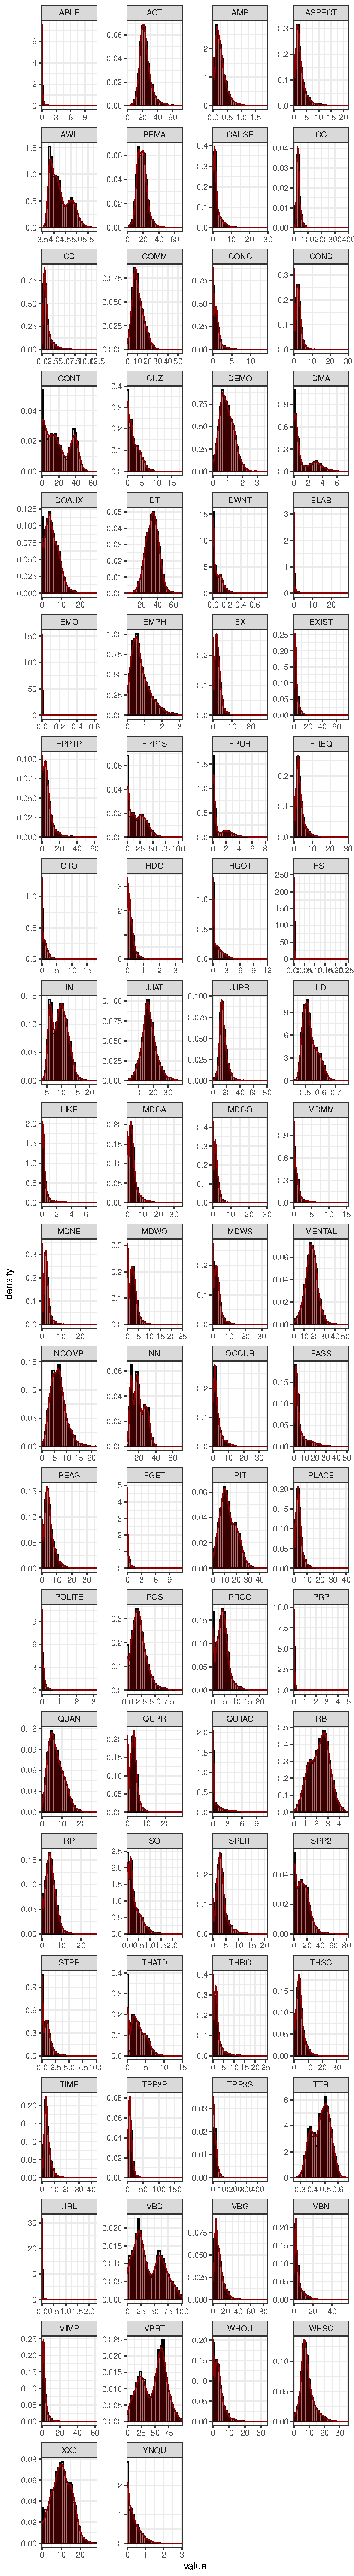
\includegraphics{F_Ch7_DataPrep_files/figure-pdf/distribution-viz-1.pdf}

\begin{Shaded}
\begin{Highlighting}[]
\CommentTok{\#ggsave(here("plots", "DensityPlotsAllVariables.svg"), width = 15, height = 49)}
\end{Highlighting}
\end{Shaded}

\subsection{Feature removal}\label{feature-removal-1}

A number of features were removed from the dataset as they are not
linguistically interpretable. In the case of the TEC, this included the
variable CD because numbers spelt out as digits were removed from the
textbooks before these were tagged with the MFTE. In addition, the
variables LIKE and SO because these are ``bin'' features included in the
output of the MFTE to ensure that the counts for these polysemous words
do not inflate other categories due to mistags (Le Foll 2021b).

Whenever linguistically meaningful, very low-frequency features,
features with low MSA or communalities (see chunks below) were merged.
Finally, features absent from more than third of texts were also
excluded. For the comparative analysis of TEC and the reference corpora,
the following linguistic features were excluded from the analysis due to
low dispersion:

\begin{Shaded}
\begin{Highlighting}[]
\CommentTok{\# Removal of meaningless feature: CD because numbers as digits were mostly removed from the textbooks, LIKE and SO because they are dustbin categories}
\NormalTok{ncounts }\OtherTok{\textless{}{-}}\NormalTok{ ncounts }\SpecialCharTok{|\textgreater{}} 
  \FunctionTok{select}\NormalTok{(}\SpecialCharTok{{-}}\FunctionTok{c}\NormalTok{(CD, LIKE, SO))}

\CommentTok{\# Combine problematic features into meaningful groups whenever this makes linguistic sense}
\NormalTok{ncounts }\OtherTok{\textless{}{-}}\NormalTok{ ncounts }\SpecialCharTok{|\textgreater{}} 
  \FunctionTok{mutate}\NormalTok{(}\AttributeTok{JJPR =}\NormalTok{ JJPR }\SpecialCharTok{+}\NormalTok{ ABLE, }\AttributeTok{ABLE =} \ConstantTok{NULL}\NormalTok{) }\SpecialCharTok{|\textgreater{}} 
  \FunctionTok{mutate}\NormalTok{(}\AttributeTok{PASS =}\NormalTok{ PGET }\SpecialCharTok{+}\NormalTok{ PASS, }\AttributeTok{PGET =} \ConstantTok{NULL}\NormalTok{) }\SpecialCharTok{|\textgreater{}} 
  \FunctionTok{mutate}\NormalTok{(}\AttributeTok{TPP3 =}\NormalTok{ TPP3S }\SpecialCharTok{+}\NormalTok{ TPP3P, }\AttributeTok{TPP3P =} \ConstantTok{NULL}\NormalTok{, }\AttributeTok{TPP3S =} \ConstantTok{NULL}\NormalTok{) }\SpecialCharTok{|\textgreater{}} \CommentTok{\# Merged due to TTP3P having an individual MSA \textless{} 0.5}
  \FunctionTok{mutate}\NormalTok{(}\AttributeTok{FQTI =}\NormalTok{ FREQ }\SpecialCharTok{+}\NormalTok{ TIME, }\AttributeTok{FREQ =} \ConstantTok{NULL}\NormalTok{, }\AttributeTok{TIME =} \ConstantTok{NULL}\NormalTok{) }\CommentTok{\# Merged due to TIME communality \textless{} 0.2 (see below)}

\CommentTok{\# Function to compute percentage of texts with occurrences meeting a condition}
\NormalTok{compute\_percentage }\OtherTok{\textless{}{-}} \ControlFlowTok{function}\NormalTok{(data, condition, threshold) \{}
\NormalTok{  numeric\_data }\OtherTok{\textless{}{-}} \FunctionTok{Filter}\NormalTok{(is.numeric, data)}
\NormalTok{  percentage }\OtherTok{\textless{}{-}} \FunctionTok{round}\NormalTok{(}\FunctionTok{colSums}\NormalTok{(condition[, }\FunctionTok{sapply}\NormalTok{(numeric\_data, is.numeric)])}\SpecialCharTok{/}\FunctionTok{nrow}\NormalTok{(data) }\SpecialCharTok{*} \DecValTok{100}\NormalTok{, }\DecValTok{2}\NormalTok{)}
\NormalTok{  percentage }\OtherTok{\textless{}{-}} \FunctionTok{as.data.frame}\NormalTok{(percentage)}
  \FunctionTok{colnames}\NormalTok{(percentage) }\OtherTok{\textless{}{-}} \StringTok{"Percentage"}
\NormalTok{  percentage }\OtherTok{\textless{}{-}}\NormalTok{ percentage }\SpecialCharTok{|\textgreater{}} 
    \FunctionTok{filter}\NormalTok{(}\SpecialCharTok{!}\FunctionTok{is.na}\NormalTok{(Percentage)) }\SpecialCharTok{|\textgreater{}}
    \FunctionTok{rownames\_to\_column}\NormalTok{() }\SpecialCharTok{|\textgreater{}}
    \FunctionTok{arrange}\NormalTok{(Percentage)}
  \ControlFlowTok{if}\NormalTok{ (}\SpecialCharTok{!}\FunctionTok{missing}\NormalTok{(threshold)) \{}
\NormalTok{    percentage }\OtherTok{\textless{}{-}}\NormalTok{ percentage }\SpecialCharTok{|\textgreater{}} 
      \FunctionTok{filter}\NormalTok{(Percentage }\SpecialCharTok{\textgreater{}}\NormalTok{ threshold)}
\NormalTok{  \}}
  \FunctionTok{return}\NormalTok{(percentage)}
\NormalTok{\}}

\CommentTok{\# Calculate percentage of texts with 0 occurrences of each feature}
\NormalTok{zero\_features }\OtherTok{\textless{}{-}} \FunctionTok{compute\_percentage}\NormalTok{(ncounts, ncounts }\SpecialCharTok{==} \DecValTok{0}\NormalTok{, }\FloatTok{66.6}\NormalTok{)}
\NormalTok{zero\_features }\SpecialCharTok{|\textgreater{}} 
  \FunctionTok{kable}\NormalTok{(}\AttributeTok{col.names =} \FunctionTok{c}\NormalTok{(}\StringTok{"Feature"}\NormalTok{, }\StringTok{"\% texts with zero occurrences"}\NormalTok{))}
\end{Highlighting}
\end{Shaded}

\begin{longtable}[]{@{}lr@{}}
\toprule\noalign{}
Feature & \% texts with zero occurrences \\
\midrule\noalign{}
\endhead
\bottomrule\noalign{}
\endlastfoot
PRP & 85.34 \\
URL & 93.03 \\
EMO & 98.98 \\
HST & 99.55 \\
\end{longtable}

\begin{Shaded}
\begin{Highlighting}[]
\CommentTok{\# Drop variables with low document frequency}
\NormalTok{ncounts2 }\OtherTok{\textless{}{-}} \FunctionTok{select}\NormalTok{(ncounts, }\SpecialCharTok{{-}}\FunctionTok{one\_of}\NormalTok{(zero\_features}\SpecialCharTok{$}\NormalTok{rowname))}
\end{Highlighting}
\end{Shaded}

These feature removal operations resulted in a feature set of 71
linguistic variables.

\subsection{Identifying outlier texts}\label{identifying-outlier-texts}

All normalised frequencies were normalised to identify any potential
outlier texts.

\begin{Shaded}
\begin{Highlighting}[]
\CommentTok{\# First scale the normalised counts (z{-}standardisation) to be able to compare the various features}
\NormalTok{zcounts }\OtherTok{\textless{}{-}}\NormalTok{ ncounts2 }\SpecialCharTok{|\textgreater{}}
  \FunctionTok{select}\NormalTok{(}\SpecialCharTok{{-}}\NormalTok{Words) }\SpecialCharTok{|\textgreater{}} 
  \FunctionTok{keep}\NormalTok{(is.numeric) }\SpecialCharTok{|\textgreater{}} 
  \FunctionTok{scale}\NormalTok{()}

\CommentTok{\# If necessary, remove any outliers at this stage.}
\NormalTok{data }\OtherTok{\textless{}{-}} \FunctionTok{cbind}\NormalTok{(ncounts2[,}\DecValTok{1}\SpecialCharTok{:}\DecValTok{8}\NormalTok{], }\FunctionTok{as.data.frame}\NormalTok{(zcounts))}
\NormalTok{outliers }\OtherTok{\textless{}{-}}\NormalTok{ data }\SpecialCharTok{|\textgreater{}} 
 \FunctionTok{filter}\NormalTok{(}\FunctionTok{if\_any}\NormalTok{(}\FunctionTok{where}\NormalTok{(is.numeric) }\SpecialCharTok{\&} \SpecialCharTok{!}\NormalTok{Words,  }\AttributeTok{.fns =} \ControlFlowTok{function}\NormalTok{(x)\{x }\SpecialCharTok{\textgreater{}} \DecValTok{8}\NormalTok{\}))  }\SpecialCharTok{|\textgreater{}}
  \FunctionTok{select}\NormalTok{(Filename, Corpus, Register, Words) }
\end{Highlighting}
\end{Shaded}

The following outlier texts were identified according to the above
conditions and excluded in subsequent analyses.

\begin{Shaded}
\begin{Highlighting}[]
\CommentTok{\# These are potential outlier texts :}
\NormalTok{outliers }\SpecialCharTok{|\textgreater{}} 
  \FunctionTok{kable}\NormalTok{(}\AttributeTok{col.names =} \FunctionTok{c}\NormalTok{(}\StringTok{"Filename"}\NormalTok{, }\StringTok{"Corpus"}\NormalTok{, }\StringTok{"Register"}\NormalTok{, }\StringTok{"\# words"}\NormalTok{))}
\end{Highlighting}
\end{Shaded}

\begin{longtable}[]{@{}
  >{\raggedright\arraybackslash}p{(\columnwidth - 6\tabcolsep) * \real{0.7045}}
  >{\raggedright\arraybackslash}p{(\columnwidth - 6\tabcolsep) * \real{0.1364}}
  >{\raggedright\arraybackslash}p{(\columnwidth - 6\tabcolsep) * \real{0.0985}}
  >{\raggedleft\arraybackslash}p{(\columnwidth - 6\tabcolsep) * \real{0.0606}}@{}}
\toprule\noalign{}
\begin{minipage}[b]{\linewidth}\raggedright
Filename
\end{minipage} & \begin{minipage}[b]{\linewidth}\raggedright
Corpus
\end{minipage} & \begin{minipage}[b]{\linewidth}\raggedright
Register
\end{minipage} & \begin{minipage}[b]{\linewidth}\raggedleft
\# words
\end{minipage} \\
\midrule\noalign{}
\endhead
\bottomrule\noalign{}
\endlastfoot
POC\_4e\_Spoken\_0007.txt & Textbook.English & Conversation & 750 \\
Solutions\_Elementary\_ELF\_Spoken\_0013.txt & Textbook.English &
Conversation & 931 \\
EIM\_Starter\_Informative\_0004.txt & Textbook.English & Informative &
534 \\
GreenLine\_1\_Spoken\_0003.txt & Textbook.English & Conversation &
970 \\
Access\_1\_Spoken\_0011.txt & Textbook.English & Conversation & 784 \\
Achievers\_B1\_Informative\_0003.txt & Textbook.English & Informative &
926 \\
EIM\_Starter\_Spoken\_0002.txt & Textbook.English & Conversation &
824 \\
GreenLine\_1\_Spoken\_0008.txt & Textbook.English & Conversation &
876 \\
JTT\_3\_Informative\_0003.txt & Textbook.English & Informative & 699 \\
GreenLine\_1\_Spoken\_0010.txt & Textbook.English & Conversation &
701 \\
EIM\_1\_Spoken\_0012.txt & Textbook.English & Conversation & 640 \\
NGL\_1\_Spoken\_0013.txt & Textbook.English & Conversation & 940 \\
NGL\_3\_Spoken\_0018.txt & Textbook.English & Conversation & 751 \\
Solutions\_Intermediate\_Spoken\_0029.txt & Textbook.English &
Conversation & 672 \\
NGL\_1\_Spoken\_0012.txt & Textbook.English & Conversation & 910 \\
GreenLine\_1\_Spoken\_0006.txt & Textbook.English & Conversation &
622 \\
GreenLine\_2\_Spoken\_0004.txt & Textbook.English & Conversation &
1102 \\
Access\_2\_Spoken\_0023.txt & Textbook.English & Conversation & 875 \\
HT\_4\_Informative\_0006.txt & Textbook.English & Informative & 513 \\
Solutions\_Intermediate\_Informative\_0017.txt & Textbook.English &
Informative & 816 \\
EIM\_1\_Spoken\_0013.txt & Textbook.English & Conversation & 967 \\
Solutions\_Elementary\_ELF\_Spoken\_0021.txt & Textbook.English &
Conversation & 846 \\
Solutions\_Intermediate\_Plus\_Spoken\_0022.txt & Textbook.English &
Conversation & 596 \\
Access\_2\_Spoken\_0028.txt & Textbook.English & Conversation & 813 \\
NGL\_1\_Spoken\_0005.txt & Textbook.English & Conversation & 1020 \\
Solutions\_Elementary\_ELF\_Spoken\_0016.txt & Textbook.English &
Conversation & 871 \\
Solutions\_Pre-Intermediate\_ELF\_Spoken\_0007.txt & Textbook.English &
Conversation & 630 \\
Solutions\_Intermediate\_Informative\_0013.txt & Textbook.English &
Informative & 770 \\
GreenLine\_2\_Spoken\_0003.txt & Textbook.English & Conversation &
850 \\
HT\_4\_Spoken\_0010.txt & Textbook.English & Conversation & 727 \\
Solutions\_Elementary\_Informative\_0003.txt & Textbook.English &
Informative & 1051 \\
Access\_2\_Informative\_0001.txt & Textbook.English & Informative &
655 \\
Solutions\_Elementary\_Informative\_0010.txt & Textbook.English &
Informative & 708 \\
GreenLine\_1\_Informative\_0001.txt & Textbook.English & Informative &
731 \\
Access\_2\_Spoken\_0002.txt & Textbook.English & Conversation & 572 \\
Solutions\_Intermediate\_Spoken\_0019.txt & Textbook.English &
Conversation & 1024 \\
Access\_3\_Informative\_0003.txt & Textbook.English & Informative &
1000 \\
Access\_1\_Spoken\_0019.txt & Textbook.English & Conversation & 701 \\
Access\_2\_Spoken\_0013.txt & Textbook.English & Conversation & 981 \\
Solutions\_Intermediate\_Plus\_Informative\_0014.txt & Textbook.English
& Informative & 537 \\
Revision\_World\_GCSE\_10525362\_literary-terms.txt & Informative.Teens
& Informative & 790 \\
Revision\_World\_GCSE\_10528697\_p6-physics-radioactive-materials.txt &
Informative.Teens & Informative & 1015 \\
Science\_Tech\_Kinds\_NZ\_10382383\_math.txt & Informative.Teens &
Informative & 522 \\
Science\_for\_students\_10064820\_scientists-say-metabolism.txt &
Informative.Teens & Informative & 895 \\
Science\_Tech\_Kinds\_NZ\_10382388\_recycling.txt & Informative.Teens &
Informative & 666 \\
History\_Kids\_BBC\_10404337\_go\_furthers.txt & Informative.Teens &
Informative & 620 \\
Science\_Tech\_Kinds\_NZ\_10382391\_sports.txt & Informative.Teens &
Informative & 657 \\
Teen\_Kids\_News\_10402607\_so-you-want-to-be-an-archivist.txt &
Informative.Teens & Informative & 763 \\
Science\_Tech\_Kinds\_NZ\_10382234\_biology.txt & Informative.Teens &
Informative & 843 \\
Science\_Tech\_Kinds\_NZ\_10382372\_astronomy.txt & Informative.Teens &
Informative & 900 \\
Dogo\_News\_file10060404\_banana-plant-extract-may-be-the-key-to-slower-melting-ice-cream.txt
& Informative.Teens & Informative & 611 \\
Science\_Tech\_Kinds\_NZ\_10382667\_countries.txt & Informative.Teens &
Informative & 717 \\
Quatr\_us\_file10390777\_quick-summary-geological-erashtm.txt &
Informative.Teens & Informative & 643 \\
Science\_Tech\_Kinds\_NZ\_10382873\_physics.txt & Informative.Teens &
Informative & 722 \\
Science\_Tech\_Kinds\_NZ\_10382382\_light.txt & Informative.Teens &
Informative & 639 \\
Factmonster\_10053687\_august-13.txt & Informative.Teens & Informative &
523 \\
Revision\_World\_GCSE\_10526703\_limited-companies.txt &
Informative.Teens & Informative & 714 \\
Revision\_World\_GCSE\_10529637\_transition-metals.txt &
Informative.Teens & Informative & 787 \\
Quatr\_us\_10390856\_early-african-historyhtm.txt & Informative.Teens &
Informative & 1136 \\
History\_Kids\_BBC\_10401873\_ff6\_sicilylandingss.txt &
Informative.Teens & Informative & 813 \\
Quatr\_us\_10394250\_harappan.txt & Informative.Teens & Informative &
651 \\
Ducksters\_10398301\_iraqphp.txt & Informative.Teens & Informative &
657 \\
History\_Kids\_BBC\_10403171\_death\_sakkara\_gallery\_04s.txt &
Informative.Teens & Informative & 844 \\
Revision\_World\_GCSE\_10528246\_agricultural-change.txt &
Informative.Teens & Informative & 789 \\
Revision\_World\_GCSE\_10528086\_uk-government-judiciary.txt &
Informative.Teens & Informative & 1019 \\
Revision\_World\_GCSE\_10529794\_definitions.txt & Informative.Teens &
Informative & 904 \\
Encyclopedia\_Kinds\_au\_10085347\_Nobel\_Prize\_in\_Chemistry.txt &
Informative.Teens & Informative & 598 \\
Science\_for\_students\_10064875\_questions-big-melt-earths-ice-sheets-are-under-attack.txt
& Informative.Teens & Informative & 685 \\
Teen\_Kids\_News\_10403301\_golden-globe-winners-2019-the-complete-list.txt
& Informative.Teens & Informative & 800 \\
Science\_Tech\_Kinds\_NZ\_10382201\_projects.txt & Informative.Teens &
Informative & 947 \\
Revision\_World\_GCSE\_10529753\_probability.txt & Informative.Teens &
Informative & 816 \\
Encyclopedia\_Kinds\_au\_10085531\_Complex\_analysis.txt &
Informative.Teens & Informative & 735 \\
History\_Kids\_BBC\_10401890\_ff7\_ddays.txt & Informative.Teens &
Informative & 759 \\
History\_Kids\_BBC\_10403434s.txt & Informative.Teens & Informative &
732 \\
History\_Kids\_BBC\_10401872\_ff6\_italys.txt & Informative.Teens &
Informative & 786 \\
Science\_Tech\_Kinds\_NZ\_10382371\_amazing.txt & Informative.Teens &
Informative & 629 \\
Quatr\_us\_10391129\_athabascan.txt & Informative.Teens & Informative &
637 \\
Encyclopedia\_Kinds\_au\_10085355\_20th\_century.txt & Informative.Teens
& Informative & 864 \\
Dogo\_News\_10060755\_luxury-space-hotel-promises-guests-a-truly-out-of-this-world-vacation.txt
& Informative.Teens & Informative & 722 \\
Revision\_World\_GCSE\_10528072\_nationalism-practice.txt &
Informative.Teens & Informative & 776 \\
Quatr\_us\_10390861\_quatr-us-privacy-policyhtm.txt & Informative.Teens
& Informative & 960 \\
History\_Kids\_BBC\_10401909\_ff7\_bulges.txt & Informative.Teens &
Informative & 732 \\
History\_kids\_10381259\_timeline-of-mesopotamia.txt & Informative.Teens
& Informative & 768 \\
Revision\_World\_GCSE\_10528123\_gender-written-textual-analysis-framework.txt
& Informative.Teens & Informative & 905 \\
Science\_Tech\_Kinds\_NZ\_10386406\_floods.txt & Informative.Teens &
Informative & 580 \\
Revision\_World\_GCSE\_10529693\_advantages.txt & Informative.Teens &
Informative & 782 \\
Science\_Tech\_Kinds\_NZ\_10382378\_geography.txt & Informative.Teens &
Informative & 761 \\
Science\_Tech\_Kinds\_NZ\_10382374\_earth.txt & Informative.Teens &
Informative & 726 \\
Science\_for\_students\_10066286\_watering-plants-wastewater-can-spread-germs.txt
& Informative.Teens & Informative & 836 \\
Science\_Tech\_Kinds\_NZ\_10382393\_water.txt & Informative.Teens &
Informative & 856 \\
World\_Dteen\_10406069\_website\_policies.txt & Informative.Teens &
Informative & 995 \\
Science\_Tech\_Kinds\_NZ\_10382384\_metals.txt & Informative.Teens &
Informative & 669 \\
Dogo\_News\_10062028\_puppy-bowl-14-promises-viewers-a-paw-some-time-on-super-bowl-sunday.txt
& Informative.Teens & Informative & 581 \\
History\_Kids\_BBC\_10404730\_go\_furthers.txt & Informative.Teens &
Informative & 611 \\
Science\_Tech\_Kinds\_NZ\_10382385\_nature.txt & Informative.Teens &
Informative & 722 \\
Science\_for\_students\_10065015\_scientists-say-dna-sequencing.txt &
Informative.Teens & Informative & 953 \\
Quatr\_us\_file10390817\_conifers-pine-trees-gymnospermshtm.txt &
Informative.Teens & Informative & 533 \\
TweenTribute\_10051509\_it-true-elephants-cant-jump.txt &
Informative.Teens & Informative & 790 \\
Revision\_World\_GCSE\_10528494\_application-software.txt &
Informative.Teens & Informative & 855 \\
Revision\_World\_GCSE\_10529581\_different-types-questions-examinations.txt
& Informative.Teens & Informative & 742 \\
Dogo\_News\_10061669\_the-chinese-city-of-chengdu-may-soon-be-home-to-multiple-moons.txt
& Informative.Teens & Informative & 614 \\
Ducksters\_10398306\_geography\_of\_ancient\_chinaphp.txt &
Informative.Teens & Informative & 638 \\
Science\_for\_students\_10065144\_scientists-say-multiverse.txt &
Informative.Teens & Informative & 712 \\
Science\_Tech\_Kinds\_NZ\_10382211\_images.txt & Informative.Teens &
Informative & 793 \\
Factmonster\_10053754\_may-18.txt & Informative.Teens & Informative &
497 \\
World\_Dteen\_10406047\_AboutWORLDteen.txt & Informative.Teens &
Informative & 1053 \\
Ducksters\_10398078\_first\_new\_dealphp.txt & Informative.Teens &
Informative & 649 \\
Revision\_World\_GCSE\_10526926\_economies-scale.txt & Informative.Teens
& Informative & 621 \\
Factmonster\_10053201\_september-03.txt & Informative.Teens &
Informative & 445 \\
Science\_Tech\_Kinds\_NZ\_10387183\_calciumcarbonates.txt &
Informative.Teens & Informative & 804 \\
Science\_Tech\_Kinds\_NZ\_10382380\_health.txt & Informative.Teens &
Informative & 694 \\
Revision\_World\_GCSE\_10529587\_sources-finance.txt & Informative.Teens
& Informative & 665 \\
Quatr\_us\_10393444\_fishing.txt & Informative.Teens & Informative &
656 \\
Ducksters\_10398315\_glossary\_and\_termsphp.txt & Informative.Teens &
Informative & 684 \\
S5AA.txt & Spoken.BNC2014 & Conversation & 1869 \\
\end{longtable}

We check that that outlier texts are not particularly long or short
texts by looking at the distribution of text/file length of the
outliers.

\begin{Shaded}
\begin{Highlighting}[]
\FunctionTok{summary}\NormalTok{(outliers}\SpecialCharTok{$}\NormalTok{Words)}
\end{Highlighting}
\end{Shaded}

\begin{verbatim}
   Min. 1st Qu.  Median    Mean 3rd Qu.    Max. 
  445.0   655.5   751.0   773.6   860.0  1869.0 
\end{verbatim}

\begin{Shaded}
\begin{Highlighting}[]
\FunctionTok{hist}\NormalTok{(outliers}\SpecialCharTok{$}\NormalTok{Words, }\AttributeTok{breaks =} \DecValTok{30}\NormalTok{)}
\end{Highlighting}
\end{Shaded}

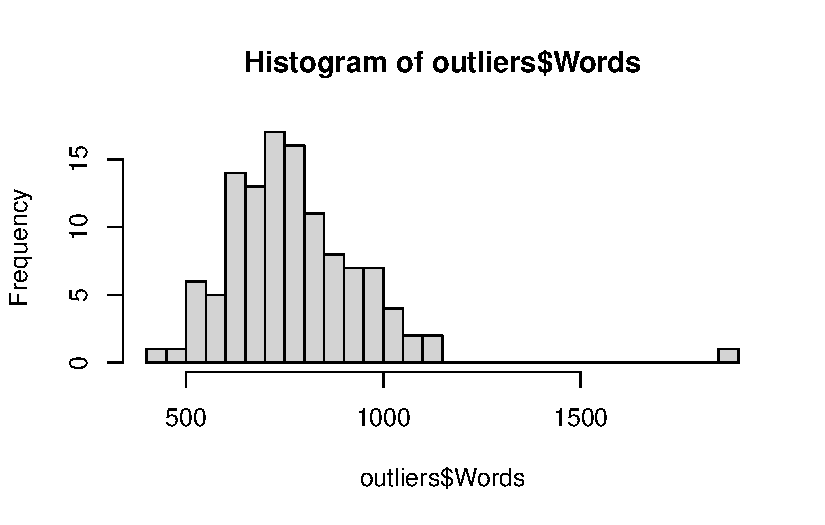
\includegraphics{F_Ch7_DataPrep_files/figure-pdf/unnamed-chunk-7-1.pdf}

We also check the distribution of outlier texts across the four corpora.
The majority come from the Info Teens corpus, though quite a few are
also from the TEC.

\begin{Shaded}
\begin{Highlighting}[]
\FunctionTok{summary}\NormalTok{(outliers}\SpecialCharTok{$}\NormalTok{Corpus) }\SpecialCharTok{|\textgreater{}} 
  \FunctionTok{kable}\NormalTok{(}\AttributeTok{col.names =} \FunctionTok{c}\NormalTok{(}\StringTok{"(Sub)corpus"}\NormalTok{, }\StringTok{"\# outlier texts"}\NormalTok{))}
\end{Highlighting}
\end{Shaded}

\begin{longtable}[]{@{}lr@{}}
\toprule\noalign{}
(Sub)corpus & \# outlier texts \\
\midrule\noalign{}
\endhead
\bottomrule\noalign{}
\endlastfoot
Textbook.English & 40 \\
Informative.Teens & 74 \\
Spoken.BNC2014 & 1 \\
Youth.Fiction & 0 \\
\end{longtable}

\begin{Shaded}
\begin{Highlighting}[]
\CommentTok{\# Report on the manual check of a sample of these outliers:}

\CommentTok{\# Encyclopedia\_Kinds\_au\_10085347\_Nobel\_Prize\_in\_Chemistry.txt is essentially a list of Nobel prize winners but with some additional information. In other words, not a bad representative of the type of texts of the Info Teen corpus.}
\CommentTok{\# Solutions\_Elementary\_ELF\_Spoken\_0013 {-}{-}\textgreater{} Has a lot of "going to" constructions because they are learnt in this chapter but is otherwise a well{-}formed text.}
\CommentTok{\# Teen\_Kids\_News\_10403972\_a{-}brief{-}history{-}of{-}white{-}house{-}weddings {-}{-}\textgreater{} No issues}
\CommentTok{\# Teen\_Kids\_News\_10403301\_golden{-}globe{-}winners{-}2019{-}the{-}complete{-}list {-}{-}\textgreater{} Similar to the Nobel prize laureates text.}
\CommentTok{\# Revision\_World\_GCSE\_10528123\_gender{-}written{-}textual{-}analysis{-}framework {-}{-}\textgreater{} Text includes bullet points tokenised as the letter "o" but otherwise a fairly typical informative text.}

\CommentTok{\# Removing the outliers at the request of the reviewers (but comparisons of models including the outliers showed that the results are very similar):}
\NormalTok{ncounts3 }\OtherTok{\textless{}{-}}\NormalTok{ ncounts2 }\SpecialCharTok{|\textgreater{}} 
  \FunctionTok{filter}\NormalTok{(}\SpecialCharTok{!}\NormalTok{Filename }\SpecialCharTok{\%in\%}\NormalTok{ outliers}\SpecialCharTok{$}\NormalTok{Filename)}

\CommentTok{\#saveRDS(ncounts3, here("data", "processed", "ncounts3\_3Reg.rds")) \# Last saved 6 March 2024}
\end{Highlighting}
\end{Shaded}

This resulted in 4,980 texts/files being included in the comparative
model of Textbook English vs.~`real-world' English. These standardised
feature frequencies were distributed as follows:

\begin{Shaded}
\begin{Highlighting}[]
\NormalTok{zcounts3 }\OtherTok{\textless{}{-}}\NormalTok{ ncounts3 }\SpecialCharTok{|\textgreater{}}
  \FunctionTok{select}\NormalTok{(}\SpecialCharTok{{-}}\NormalTok{Words) }\SpecialCharTok{|\textgreater{}} 
  \FunctionTok{keep}\NormalTok{(is.numeric) }\SpecialCharTok{|\textgreater{}} 
  \FunctionTok{scale}\NormalTok{()}

\FunctionTok{boxplot}\NormalTok{(zcounts3, }\AttributeTok{las =} \DecValTok{3}\NormalTok{, }\AttributeTok{main =} \StringTok{"z{-}scores"}\NormalTok{) }\CommentTok{\# Slow}
\end{Highlighting}
\end{Shaded}

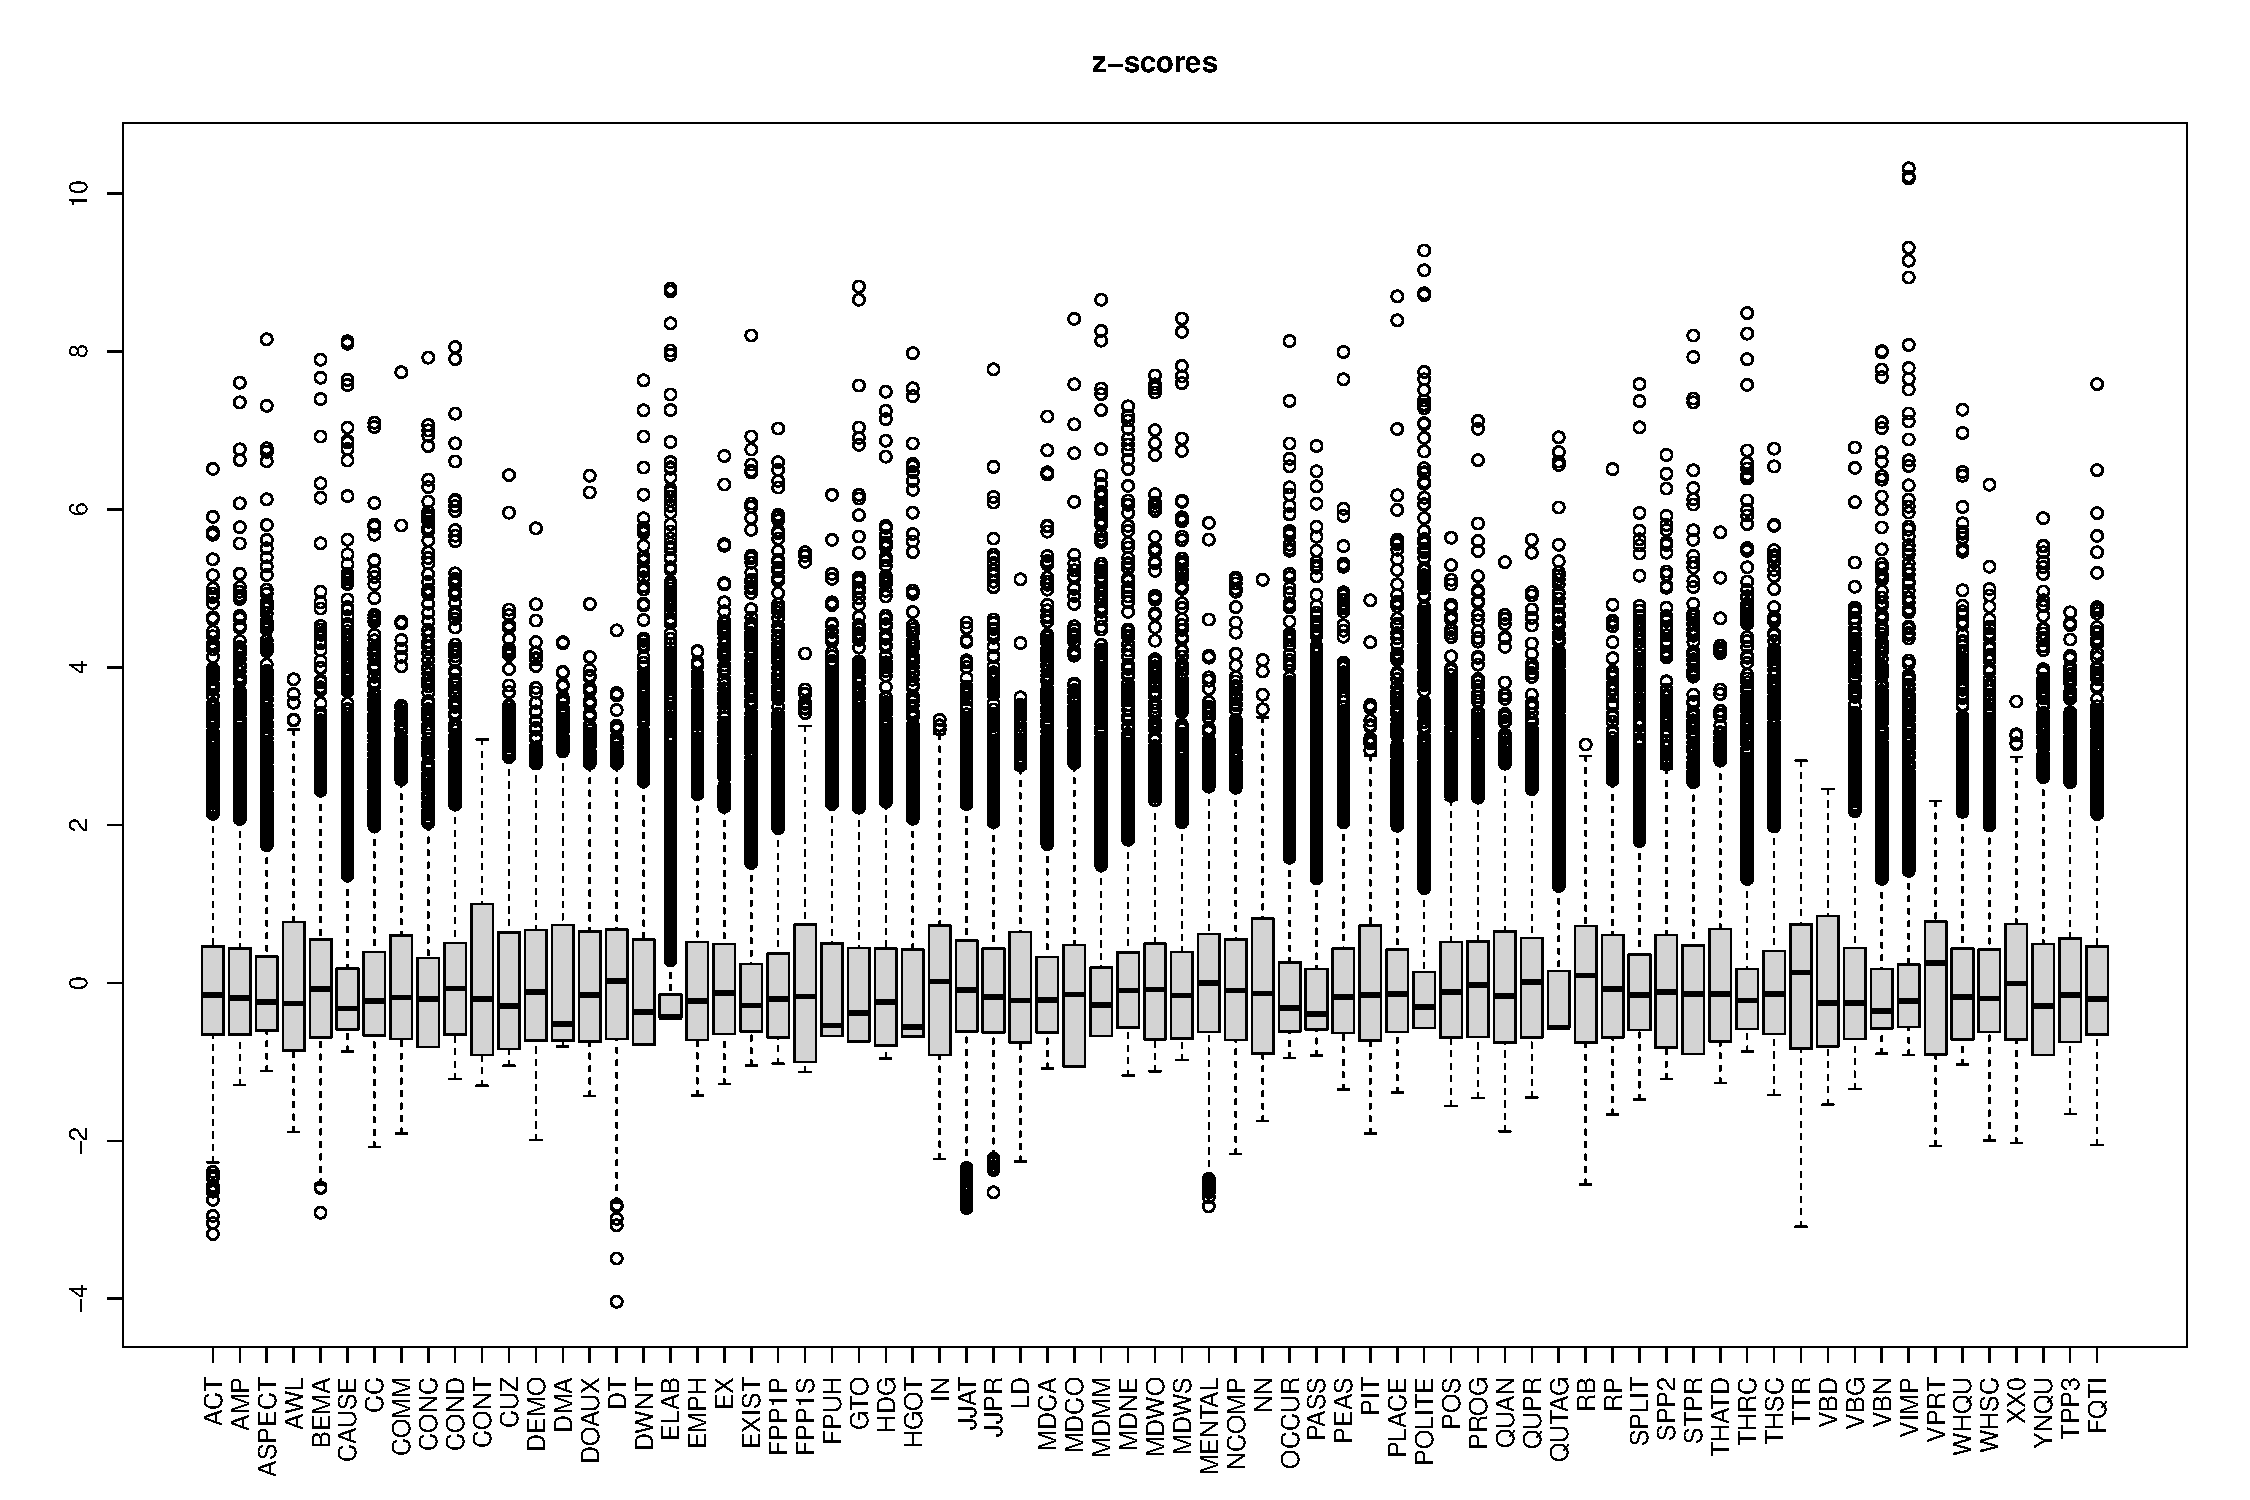
\includegraphics{F_Ch7_DataPrep_files/figure-pdf/z-transformed-distributions-1.pdf}

\subsection{Signed log
transformation}\label{signed-log-transformation-1}

A signed logarithmic transformation was applied to (further) deskew the
feature distributions (see Diwersy, Evert, and Neumann 2014; Neumann and
Evert 2021).

The signed log transformation function was inspired by the SignedLog
function proposed in
\url{https://cran.r-project.org/web/packages/DataVisualizations/DataVisualizations.pdf}.

\begin{Shaded}
\begin{Highlighting}[]
\NormalTok{signed.log }\OtherTok{\textless{}{-}} \ControlFlowTok{function}\NormalTok{(x) \{}\FunctionTok{sign}\NormalTok{(x)}\SpecialCharTok{*}\FunctionTok{log}\NormalTok{(}\FunctionTok{abs}\NormalTok{(x)}\SpecialCharTok{+}\DecValTok{1}\NormalTok{)\}}

\CommentTok{\# Standardise first, then sign log transform}
\NormalTok{zlogcounts }\OtherTok{\textless{}{-}} \FunctionTok{signed.log}\NormalTok{(zcounts3) }
\end{Highlighting}
\end{Shaded}

The new feature distributions are visualised below.

\begin{Shaded}
\begin{Highlighting}[]
\NormalTok{zlogcounts }\SpecialCharTok{|\textgreater{}}
  \FunctionTok{as.data.frame}\NormalTok{() }\SpecialCharTok{|\textgreater{}} 
  \FunctionTok{gather}\NormalTok{() }\SpecialCharTok{|\textgreater{}} \CommentTok{\# This function from tidyr converts a selection of variables into two variables: a key and a value. The key contains the names of the original variable and the value the data. This means we can then use the facet\_wrap function from ggplot2}
  \FunctionTok{ggplot}\NormalTok{(}\FunctionTok{aes}\NormalTok{(value, }\FunctionTok{after\_stat}\NormalTok{(density))) }\SpecialCharTok{+}
  \FunctionTok{theme\_bw}\NormalTok{() }\SpecialCharTok{+}
  \FunctionTok{facet\_wrap}\NormalTok{(}\SpecialCharTok{\textasciitilde{}}\NormalTok{ key, }\AttributeTok{scales =} \StringTok{"free"}\NormalTok{, }\AttributeTok{ncol =} \DecValTok{4}\NormalTok{) }\SpecialCharTok{+}
  \FunctionTok{scale\_x\_continuous}\NormalTok{(}\AttributeTok{expand=}\FunctionTok{c}\NormalTok{(}\DecValTok{0}\NormalTok{,}\DecValTok{0}\NormalTok{)) }\SpecialCharTok{+}
  \FunctionTok{scale\_y\_continuous}\NormalTok{(}\AttributeTok{limits =} \FunctionTok{c}\NormalTok{(}\DecValTok{0}\NormalTok{,}\ConstantTok{NA}\NormalTok{)) }\SpecialCharTok{+}
  \FunctionTok{geom\_histogram}\NormalTok{(}\AttributeTok{bins =} \DecValTok{30}\NormalTok{, }\AttributeTok{colour=} \StringTok{"black"}\NormalTok{, }\AttributeTok{fill =} \StringTok{"grey"}\NormalTok{) }\SpecialCharTok{+}
  \FunctionTok{geom\_density}\NormalTok{(}\AttributeTok{colour =} \StringTok{"darkred"}\NormalTok{, }\AttributeTok{weight =} \DecValTok{2}\NormalTok{, }\AttributeTok{fill=}\StringTok{"darkred"}\NormalTok{, }\AttributeTok{alpha =}\NormalTok{ .}\DecValTok{4}\NormalTok{)}
\end{Highlighting}
\end{Shaded}

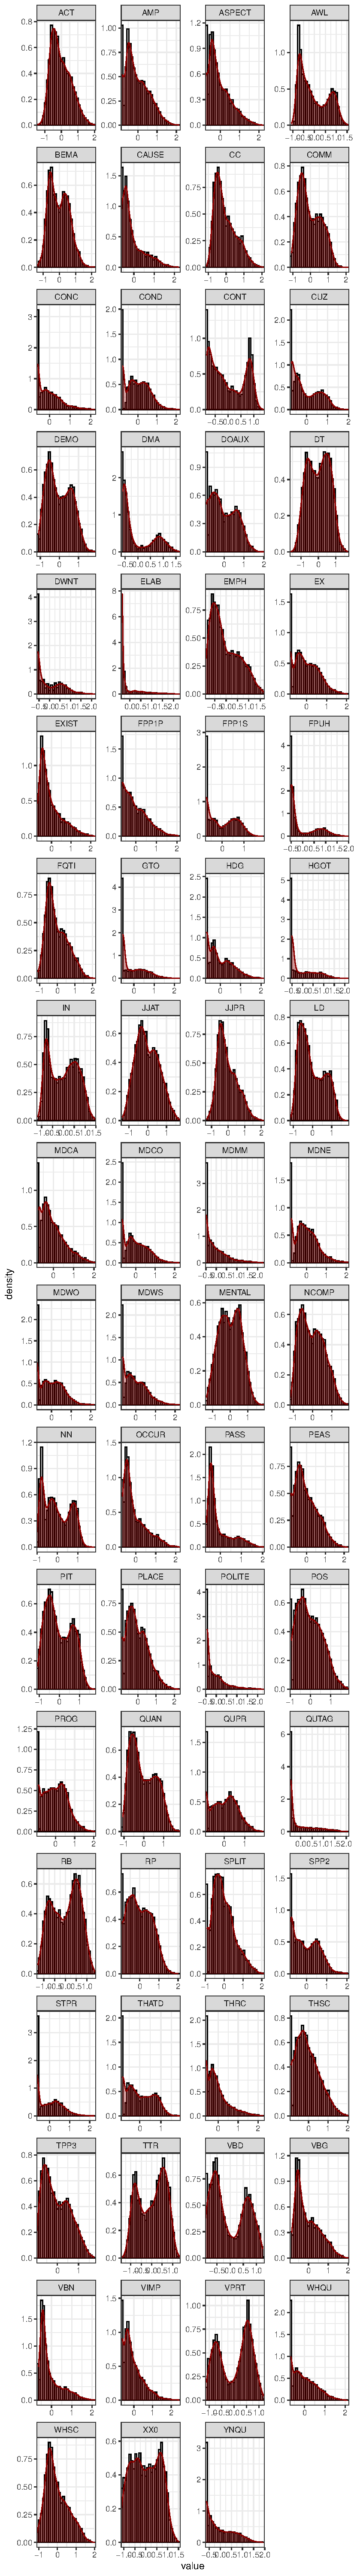
\includegraphics{F_Ch7_DataPrep_files/figure-pdf/signed.log.transformation-distributions-1.pdf}

\begin{Shaded}
\begin{Highlighting}[]
\CommentTok{\#ggsave(here("plots", "DensityPlotsAllVariablesSignedLog.svg"), width = 15, height = 49)}
\end{Highlighting}
\end{Shaded}

\subsection{Merging of data for MDA}\label{merging-of-data-for-mda}

\begin{Shaded}
\begin{Highlighting}[]
\NormalTok{zlogcounts }\OtherTok{\textless{}{-}} \FunctionTok{readRDS}\NormalTok{(}\FunctionTok{here}\NormalTok{(}\StringTok{"data"}\NormalTok{, }\StringTok{"processed"}\NormalTok{, }\StringTok{"zlogcounts\_3Reg.rds"}\NormalTok{)) }
\CommentTok{\#nrow(zlogcounts)}
\CommentTok{\#colnames(zlogcounts)}

\NormalTok{ncounts3 }\OtherTok{\textless{}{-}} \FunctionTok{readRDS}\NormalTok{(}\FunctionTok{here}\NormalTok{(}\StringTok{"data"}\NormalTok{, }\StringTok{"processed"}\NormalTok{, }\StringTok{"ncounts3\_3Reg.rds"}\NormalTok{))}
\CommentTok{\#nrow(ncounts3)}
\CommentTok{\#colnames(ncounts3)}

\NormalTok{data }\OtherTok{\textless{}{-}} \FunctionTok{cbind}\NormalTok{(ncounts3[,}\DecValTok{1}\SpecialCharTok{:}\DecValTok{8}\NormalTok{], }\FunctionTok{as.data.frame}\NormalTok{(zlogcounts))}
\CommentTok{\#saveRDS(data, here("data", "processed", "datazlogcounts\_3Reg.rds")) \# Last saved 16 March 2024}
\end{Highlighting}
\end{Shaded}

The final dataset comprises of 4,980 texts/files, divided as follows:

\begin{longtable}[]{@{}lr@{}}
\toprule\noalign{}
(Sub)corpus & \# texts/files \\
\midrule\noalign{}
\endhead
\bottomrule\noalign{}
\endlastfoot
Textbook Conversation & 565 \\
Textbook Fiction & 285 \\
Info Teens Ref. & 1337 \\
Textbook Informative & 352 \\
Spoken BNC2014 Ref. & 1250 \\
Youth Fiction Ref. & 1191 \\
\end{longtable}

\section{Testing factorability of
data}\label{testing-factorability-of-data}

\subsection{Visualisation of feature
correlations}\label{visualisation-of-feature-correlations}

We begin by visualising the correlations of the transformed feature
frequencies using the \texttt{heatmap} function of the \texttt{stats}
library. Negative correlations are rendered in blue; positive ones are
in red.

\begin{Shaded}
\begin{Highlighting}[]
\CommentTok{\# Simple heatmap in base R (inspired by Stephanie Evert\textquotesingle{}s SIGIL code)}
\NormalTok{cor.colours }\OtherTok{\textless{}{-}} \FunctionTok{c}\NormalTok{(}
  \FunctionTok{hsv}\NormalTok{(}\AttributeTok{h=}\DecValTok{2}\SpecialCharTok{/}\DecValTok{3}\NormalTok{, }\AttributeTok{v=}\DecValTok{1}\NormalTok{, }\AttributeTok{s=}\NormalTok{(}\DecValTok{10}\SpecialCharTok{:}\DecValTok{1}\NormalTok{)}\SpecialCharTok{/}\DecValTok{10}\NormalTok{), }\CommentTok{\# blue = negative correlation }
  \FunctionTok{rgb}\NormalTok{(}\DecValTok{1}\NormalTok{,}\DecValTok{1}\NormalTok{,}\DecValTok{1}\NormalTok{), }\CommentTok{\# white = no correlation }
  \FunctionTok{hsv}\NormalTok{(}\AttributeTok{h=}\DecValTok{0}\NormalTok{, }\AttributeTok{v=}\DecValTok{1}\NormalTok{, }\AttributeTok{s=}\NormalTok{(}\DecValTok{1}\SpecialCharTok{:}\DecValTok{10}\SpecialCharTok{/}\DecValTok{10}\NormalTok{))) }\CommentTok{\# red = positive correlation}

\CommentTok{\#png(here("plots", "heatmapzlogcounts.png"), width = 30, height= 30, units = "cm", res = 300)}
\FunctionTok{heatmap}\NormalTok{(}\FunctionTok{cor}\NormalTok{(zlogcounts), }
        \AttributeTok{symm=}\ConstantTok{TRUE}\NormalTok{, }
        \AttributeTok{zlim=}\FunctionTok{c}\NormalTok{(}\SpecialCharTok{{-}}\DecValTok{1}\NormalTok{,}\DecValTok{1}\NormalTok{), }
        \AttributeTok{col=}\NormalTok{cor.colours, }
        \AttributeTok{margins=}\FunctionTok{c}\NormalTok{(}\DecValTok{7}\NormalTok{,}\DecValTok{7}\NormalTok{))}
\end{Highlighting}
\end{Shaded}


\includegraphics{F_Ch7_DataPrep_files/figure-pdf/heatmap-1.pdf}

\begin{Shaded}
\begin{Highlighting}[]
\CommentTok{\#dev.off()}
\end{Highlighting}
\end{Shaded}

\subsection{Collinearity}\label{collinearity}

As a result of the normalisation unit of finite verb phrases for
verb-based features, the present tense (VPRT) and past tense (VBD)
variables are correlated to a very high degree:

\begin{Shaded}
\begin{Highlighting}[]
\FunctionTok{cor}\NormalTok{(data}\SpecialCharTok{$}\NormalTok{VPRT, data}\SpecialCharTok{$}\NormalTok{VBD) }\SpecialCharTok{|\textgreater{}} \FunctionTok{round}\NormalTok{(}\DecValTok{2}\NormalTok{)}
\end{Highlighting}
\end{Shaded}

\begin{verbatim}
[1] -0.97
\end{verbatim}

We therefore remove the least marked of the pair of collinear variables:
VPRT.

\begin{Shaded}
\begin{Highlighting}[]
\NormalTok{data }\OtherTok{\textless{}{-}}\NormalTok{ data }\SpecialCharTok{|\textgreater{}} 
  \FunctionTok{select}\NormalTok{(}\SpecialCharTok{{-}}\FunctionTok{c}\NormalTok{(VPRT))}
\end{Highlighting}
\end{Shaded}

\subsection{MSA}\label{msa}

\begin{Shaded}
\begin{Highlighting}[]
\NormalTok{kmo }\OtherTok{\textless{}{-}} \FunctionTok{KMO}\NormalTok{(data[,}\DecValTok{9}\SpecialCharTok{:}\FunctionTok{ncol}\NormalTok{(data)]) }\CommentTok{\# The first eight columns contain metadata.}
\end{Highlighting}
\end{Shaded}

The overall MSA value of the dataset is 0.95. The features have the
following individual MSA values (ordered from lowest to largest):

\begin{Shaded}
\begin{Highlighting}[]
\NormalTok{kmo}\SpecialCharTok{$}\NormalTok{MSAi[}\FunctionTok{order}\NormalTok{(kmo}\SpecialCharTok{$}\NormalTok{MSAi)] }\SpecialCharTok{|\textgreater{}}  \FunctionTok{round}\NormalTok{(}\DecValTok{2}\NormalTok{)}
\end{Highlighting}
\end{Shaded}

\begin{verbatim}
   AMP   COMM    POS   TPP3   JJPR  PLACE  SPLIT     DT   JJAT   VIMP   MDCO 
  0.67   0.69   0.70   0.74   0.76   0.82   0.83   0.83   0.84   0.84   0.85 
    RP     EX   THSC     LD  NCOMP   BEMA   MDWS   FQTI  FPP1P   MDCA    ACT 
  0.85   0.85   0.86   0.87   0.88   0.88   0.89   0.89   0.89   0.89   0.89 
MENTAL    VBD  FPP1S   MDMM   PEAS   CONC   MDWO   THRC     NN   COND   PROG 
  0.91   0.91   0.91   0.91   0.91   0.93   0.93   0.94   0.94   0.95   0.95 
    CC   SPP2     RB   DWNT   MDNE   WHSC   CONT   QUPR    XX0  CAUSE   WHQU 
  0.95   0.95   0.95   0.95   0.95   0.96   0.96   0.96   0.96   0.96   0.96 
   VBG    AWL POLITE   PASS    PIT  DOAUX   ELAB ASPECT    DMA   DEMO    HDG 
  0.96   0.96   0.96   0.96   0.97   0.97   0.97   0.97   0.97   0.97   0.97 
    IN   FPUH  OCCUR    CUZ   EMPH   YNQU   QUAN    TTR  QUTAG  THATD    VBN 
  0.97   0.97   0.97   0.97   0.98   0.98   0.98   0.98   0.98   0.98   0.98 
 EXIST   STPR    GTO   HGOT 
  0.98   0.99   0.99   0.99 
\end{verbatim}

We aim to remove features with an individual MSA \textless{} 0.5. All
features have individual MSAs of \textgreater{} 0.5 (but only because
TPP3P was merged into a broader category in an earlier chunk).

\subsection{Scree plot}\label{scree-plot}

Six components were originally retained on the basis of the following
screeplot, though only the first four were found to be interpretable and
were therefore included in the model.

\begin{Shaded}
\begin{Highlighting}[]
\CommentTok{\# png(here("plots", "screeplot{-}TEC{-}Ref\_3Reg.png"), width = 20, height= 12, units = "cm", res = 300)}
\FunctionTok{scree}\NormalTok{(data[,}\DecValTok{9}\SpecialCharTok{:}\FunctionTok{ncol}\NormalTok{(data)], }\AttributeTok{factors =} \ConstantTok{FALSE}\NormalTok{, }\AttributeTok{pc =} \ConstantTok{TRUE}\NormalTok{) }\CommentTok{\# }
\end{Highlighting}
\end{Shaded}

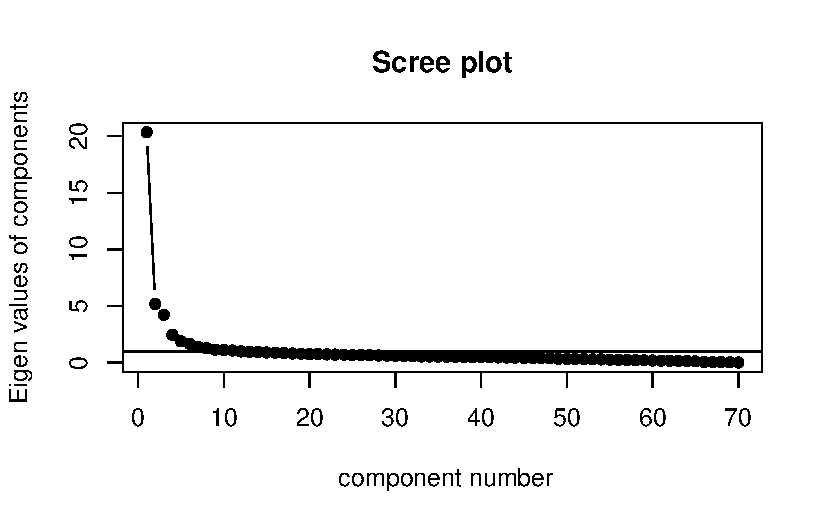
\includegraphics{F_Ch7_DataPrep_files/figure-pdf/unnamed-chunk-16-1.pdf}

\begin{Shaded}
\begin{Highlighting}[]
\CommentTok{\# dev.off()}

\CommentTok{\# Perform PCA}
\NormalTok{pca1 }\OtherTok{\textless{}{-}}\NormalTok{ psych}\SpecialCharTok{::}\FunctionTok{principal}\NormalTok{(data[}\DecValTok{9}\SpecialCharTok{:}\FunctionTok{ncol}\NormalTok{(data)], }
                         \AttributeTok{nfactors =} \DecValTok{6}\NormalTok{)}
\end{Highlighting}
\end{Shaded}

\subsection{Communalities}\label{communalities}

If features with final communalities of \textless{} 0.2 are removed,
TIME would have to be removed. TIME was therefore merged with FREQ in an
earlier chunk so that now all features have final communalities of
\textgreater{} 0.2 (note that this is a very generous threshold!).

\begin{Shaded}
\begin{Highlighting}[]
\NormalTok{pca1}\SpecialCharTok{$}\NormalTok{communality }\SpecialCharTok{|\textgreater{}} \FunctionTok{sort}\NormalTok{() }\SpecialCharTok{|\textgreater{}} \FunctionTok{round}\NormalTok{(}\DecValTok{2}\NormalTok{)}
\end{Highlighting}
\end{Shaded}

\begin{verbatim}
  DWNT   STPR   CONC   FQTI    POS ASPECT   MDNE  FPP1P   PROG   MDCO   MDMM 
  0.22   0.23   0.23   0.23   0.24   0.25   0.27   0.28   0.29   0.32   0.32 
  MDWO  SPLIT   MDWS   PEAS   QUPR    AMP  PLACE    HDG   COMM  CAUSE     EX 
  0.32   0.33   0.34   0.35   0.35   0.35   0.37   0.38   0.38   0.38   0.38 
  THSC  OCCUR   WHSC   THRC   JJAT   COND MENTAL    ACT   VIMP   ELAB  EXIST 
  0.40   0.40   0.42   0.43   0.44   0.44   0.45   0.45   0.46   0.46   0.46 
  JJPR  NCOMP     RP    GTO   DEMO   MDCA POLITE    CUZ     CC   WHQU   TPP3 
  0.46   0.48   0.49   0.50   0.50   0.52   0.52   0.53   0.57   0.58   0.58 
   VBG  THATD    PIT   BEMA  FPP1S     DT   HGOT     RB    VBN  QUTAG   EMPH 
  0.60   0.60   0.61   0.61   0.61   0.61   0.62   0.62   0.64   0.64   0.64 
  PASS    XX0   QUAN   SPP2  DOAUX    TTR   YNQU    VBD     LD   FPUH     IN 
  0.65   0.65   0.67   0.68   0.69   0.71   0.74   0.78   0.81   0.83   0.86 
  CONT    DMA    AWL     NN 
  0.89   0.89   0.91   0.93 
\end{verbatim}

\begin{Shaded}
\begin{Highlighting}[]
\CommentTok{\#saveRDS(data, here("data", "processed", "dataforPCA.rds")) \# Last saved on 6 March 2024}
\end{Highlighting}
\end{Shaded}

The final dataset entered in the analysis described in Chapter 7
therefore comprises 4,980 texts/files, each with logged standardised
normalised frequencies for 70 linguistic features.

\chapter{Data Analysis for the Model of Textbook English
vs.~`real-world'
English}\label{data-analysis-for-the-model-of-textbook-english-vs.-real-world-english}

This script documents the analysis of data from the TEC and reference
corpus data (as pre-processed in Appendix F) to arrive at the
multi-dimensional model of Textbook Englisch vs.~`real-world' English
described in Chapter 7. It generates all of the statistics and plots
included in the book, as well as many others that were used in the
analysis, but were not included in the book for reasons of space.

\section{Packages required}\label{packages-required-3}

The following packages must be installed and loaded to process the data.

\begin{Shaded}
\begin{Highlighting}[]
\CommentTok{\#renv::restore() \# Restore the project\textquotesingle{}s dependencies from the lockfile to ensure that same package versions are used as in the original thesis.}

\FunctionTok{library}\NormalTok{(caret) }\CommentTok{\# For its confusion matrix function}
\FunctionTok{library}\NormalTok{(cowplot) }\CommentTok{\# For its plot themes}
\FunctionTok{library}\NormalTok{(DescTools) }\CommentTok{\# For 95\% CI}
\FunctionTok{library}\NormalTok{(emmeans) }\CommentTok{\# For the emmeans function}
\FunctionTok{library}\NormalTok{(factoextra) }\CommentTok{\# For circular graphs of variables}
\FunctionTok{library}\NormalTok{(gtsummary) }\CommentTok{\# For nice table of summary statistics (optional)}
\FunctionTok{library}\NormalTok{(gridExtra) }\CommentTok{\# For Fig. 35}
\FunctionTok{library}\NormalTok{(here) }\CommentTok{\# For dynamic file paths}
\FunctionTok{library}\NormalTok{(ggthemes) }\CommentTok{\# For theme of factoextra plots}
\FunctionTok{library}\NormalTok{(knitr) }\CommentTok{\# Loaded to display the tables using the kable() function}
\FunctionTok{library}\NormalTok{(lme4) }\CommentTok{\# For linear regression modelling}
\FunctionTok{library}\NormalTok{(patchwork) }\CommentTok{\# To create figures with more than one plot}
\CommentTok{\#library(pca3d) \# For 3{-}D plots (not rendered in exports)}
\FunctionTok{library}\NormalTok{(PCAtools) }\CommentTok{\# For nice biplots of PCA results}
\FunctionTok{library}\NormalTok{(psych) }\CommentTok{\# For various useful stats function}
\FunctionTok{library}\NormalTok{(sjPlot) }\CommentTok{\# For model plots and tables}
\FunctionTok{library}\NormalTok{(tidyverse) }\CommentTok{\# For data wrangling}
\FunctionTok{library}\NormalTok{(visreg) }\CommentTok{\# For plots of interaction effects}

\FunctionTok{source}\NormalTok{(}\FunctionTok{here}\NormalTok{(}\StringTok{"R\_rainclouds.R"}\NormalTok{)) }\CommentTok{\# For geom\_flat\_violin rainplots}
\end{Highlighting}
\end{Shaded}

\section{Conducting the PCA}\label{conducting-the-pca}

We first import the full dataset (see Appendix F for data preparation
steps).

The following chunks can be used to perform the MDA on various subsets
of the data (see also Section 10.1.1 in the book).

\begin{enumerate}
\def\labelenumi{\roman{enumi}.}
\tightlist
\item
  Subset of the data that excludes the lower-level textbooks:
\end{enumerate}

\begin{Shaded}
\begin{Highlighting}[]
\NormalTok{data }\OtherTok{\textless{}{-}} \FunctionTok{readRDS}\NormalTok{(}\FunctionTok{here}\NormalTok{(}\StringTok{"processed\_data"}\NormalTok{, }\StringTok{"dataforPCA.rds"}\NormalTok{)) }\SpecialCharTok{|\textgreater{}}
  \FunctionTok{filter}\NormalTok{(Level }\SpecialCharTok{!=}\StringTok{"A"} \SpecialCharTok{\&}\NormalTok{ Level }\SpecialCharTok{!=} \StringTok{"B"}\NormalTok{) }\SpecialCharTok{|\textgreater{}}
  \FunctionTok{droplevels}\NormalTok{()}
\FunctionTok{summary}\NormalTok{(data}\SpecialCharTok{$}\NormalTok{Level)}
\end{Highlighting}
\end{Shaded}

\begin{enumerate}
\def\labelenumi{\roman{enumi}.}
\tightlist
\item
  Subset of the data that includes only one \texttt{Country}` subcorpus
  of the TEC (note that a detailed analysis of the German subcorpus can
  be found in (Le Foll, n.d.)):
\end{enumerate}

\begin{Shaded}
\begin{Highlighting}[]
\NormalTok{data }\OtherTok{\textless{}{-}} \FunctionTok{readRDS}\NormalTok{(}\FunctionTok{here}\NormalTok{(}\StringTok{"processed\_data"}\NormalTok{, }\StringTok{"dataforPCA.rds"}\NormalTok{)) }\SpecialCharTok{|\textgreater{}}
  \CommentTok{\#filter(Country != "France" \& Country != "Germany") |\textgreater{} \# Spain only}
  \CommentTok{\#filter(Country != "France" \& Country != "Spain") |\textgreater{} \# Germany only}
  \FunctionTok{filter}\NormalTok{(Country }\SpecialCharTok{!=} \StringTok{"Spain"} \SpecialCharTok{\&}\NormalTok{ Country }\SpecialCharTok{!=} \StringTok{"Germany"}\NormalTok{) }\SpecialCharTok{|\textgreater{}} \CommentTok{\# France only}
  \FunctionTok{droplevels}\NormalTok{()}
\FunctionTok{summary}\NormalTok{(data}\SpecialCharTok{$}\NormalTok{Country)}
\end{Highlighting}
\end{Shaded}

\begin{enumerate}
\def\labelenumi{\roman{enumi}.}
\tightlist
\item
  Random subsets of the data to test the stability of the model proposed
  in Chapter 7. Re-running this line will generate a new subset of 2/3
  of the texts randomly sampled. \texttt{set.seed(13)} was used for the
  analyses reported on in Section 10.1.1.
\end{enumerate}

\begin{Shaded}
\begin{Highlighting}[]
\FunctionTok{set.seed}\NormalTok{(}\DecValTok{13}\NormalTok{) }
\NormalTok{data }\OtherTok{\textless{}{-}} \FunctionTok{readRDS}\NormalTok{(}\FunctionTok{here}\NormalTok{(}\StringTok{"processed\_data"}\NormalTok{, }\StringTok{"dataforPCA.rds"}\NormalTok{)) }\SpecialCharTok{|\textgreater{}}
  \FunctionTok{slice\_sample}\NormalTok{(}\AttributeTok{n =} \DecValTok{4980}\SpecialCharTok{*}\FloatTok{0.6}\NormalTok{, }\AttributeTok{replace =} \ConstantTok{FALSE}\NormalTok{)}
\FunctionTok{nrow}\NormalTok{(data)}
\NormalTok{data}\SpecialCharTok{$}\NormalTok{Filename[}\DecValTok{1}\SpecialCharTok{:}\DecValTok{4}\NormalTok{]}
\CommentTok{\#Using the set.seed(13), these should be:}
\CommentTok{\#[1] HT\_4\_Spoken\_0009.txt                       }
\CommentTok{\#[2] Solutions\_Intermediate\_Plus\_Spoken\_0020.txt}
\CommentTok{\#[3] 141\_PRATCHETT1992DW13GODS\_4.txt            }
\CommentTok{\#[4] Achievers\_B2\_Informative\_0004.txt}
\end{Highlighting}
\end{Shaded}

\section{Plotting PCA results}\label{plotting-pca-results-1}

\subsection{3D plots}\label{d-plots-1}

The following chunk can be used to create projections of TEC texts on
three dimensions of the model. These plots cannot be rendered in two
dimensions and are therefore not generated in the present document. For
more information on the \texttt{pca3d} library, see:
\url{https://cran.r-project.org/web/packages/pca3d/vignettes/pca3d.pdf}.

\begin{Shaded}
\begin{Highlighting}[]
\CommentTok{\# Data preparation for 3D plots}
\FunctionTok{colnames}\NormalTok{(data) }\CommentTok{\# Checking that the features start at the 9th column}
\NormalTok{pca }\OtherTok{\textless{}{-}} \FunctionTok{prcomp}\NormalTok{(data[,}\DecValTok{9}\SpecialCharTok{:}\FunctionTok{ncol}\NormalTok{(data)], }\AttributeTok{scale.=}\ConstantTok{FALSE}\NormalTok{) }\CommentTok{\# All quantitative variables that contribute to the model}
\NormalTok{register }\OtherTok{\textless{}{-}} \FunctionTok{factor}\NormalTok{(data[,}\StringTok{"Register"}\NormalTok{]) }
\NormalTok{corpus }\OtherTok{\textless{}{-}} \FunctionTok{factor}\NormalTok{(data[,}\StringTok{"Corpus"}\NormalTok{])}
\NormalTok{subcorpus }\OtherTok{\textless{}{-}} \FunctionTok{factor}\NormalTok{(data[,}\StringTok{"Subcorpus"}\NormalTok{])}

\FunctionTok{library}\NormalTok{(pca3d)}

\FunctionTok{pca3d}\NormalTok{(pca, }\AttributeTok{group =}\NormalTok{ subcorpus,}
       \AttributeTok{components =} \DecValTok{1}\SpecialCharTok{:}\DecValTok{3}\NormalTok{,}
       \AttributeTok{components =} \DecValTok{4}\SpecialCharTok{:}\DecValTok{6}\NormalTok{,}
       \AttributeTok{show.plane=}\ConstantTok{FALSE}\NormalTok{,}
       \AttributeTok{col =}\NormalTok{ col6,}
       \AttributeTok{shape =}\NormalTok{ shapes6,}
       \AttributeTok{radius =} \FloatTok{0.7}\NormalTok{,}
       \AttributeTok{legend =} \StringTok{"right"}\NormalTok{)}

\FunctionTok{snapshotPCA3d}\NormalTok{(}\FunctionTok{here}\NormalTok{(}\StringTok{"plots"}\NormalTok{, }\StringTok{"PCA\_TxB\_3Ref\_3Dsnapshot.png"}\NormalTok{))}

\CommentTok{\# Alternative visualisation, looking at all three Textbook English registers in one colour}

\FunctionTok{pca3d}\NormalTok{(pca, }\AttributeTok{group =}\NormalTok{ corpus, }
      \AttributeTok{show.plane=}\ConstantTok{FALSE}\NormalTok{,}
      \AttributeTok{components =} \DecValTok{1}\SpecialCharTok{:}\DecValTok{3}\NormalTok{,}
      \AttributeTok{col =}\NormalTok{ col4,}
      \AttributeTok{shape =}\NormalTok{ shapes4,}
      \AttributeTok{radius =} \FloatTok{0.7}\NormalTok{,}
      \AttributeTok{legend =} \StringTok{"right"}\NormalTok{)}
\end{Highlighting}
\end{Shaded}

\section{Two-dimensional plots
(biplots)}\label{two-dimensional-plots-biplots-1}

These plots were generated using the \texttt{PCAtools} package, which
requires the data to be formatted in a rather unconventional way so it
needs to wrangled first.

\subsection{Data wrangling for
PCAtools}\label{data-wrangling-for-pcatools-1}

\begin{Shaded}
\begin{Highlighting}[]
\CommentTok{\# Data wrangling}
\NormalTok{data2 }\OtherTok{\textless{}{-}}\NormalTok{ data }\SpecialCharTok{|\textgreater{}} 
  \FunctionTok{mutate}\NormalTok{(}\AttributeTok{Source =} \FunctionTok{recode\_factor}\NormalTok{(Corpus, }\AttributeTok{Textbook.English =} \StringTok{"Textbook English (TEC)"}\NormalTok{, }\AttributeTok{Informative.Teens =} \StringTok{"Reference corpora"}\NormalTok{, }\AttributeTok{Spoken.BNC2014 =} \StringTok{"Reference corpora"}\NormalTok{, }\AttributeTok{Youth.Fiction =} \StringTok{"Reference corpora"}\NormalTok{)) }\SpecialCharTok{|\textgreater{}} 
  \FunctionTok{mutate}\NormalTok{(}\AttributeTok{Corpus =} \FunctionTok{fct\_relevel}\NormalTok{(Subcorpus, }\StringTok{"Info Teens Ref."}\NormalTok{, }\AttributeTok{after =} \DecValTok{9}\NormalTok{)) }\SpecialCharTok{|\textgreater{}}
  \FunctionTok{relocate}\NormalTok{(Source, }\AttributeTok{.after =} \StringTok{"Corpus"}\NormalTok{) }\SpecialCharTok{|\textgreater{}} 
  \FunctionTok{droplevels}\NormalTok{()}

\CommentTok{\# colnames(data2)}
\NormalTok{data2meta }\OtherTok{\textless{}{-}}\NormalTok{ data2[,}\DecValTok{1}\SpecialCharTok{:}\DecValTok{9}\NormalTok{]}
\FunctionTok{rownames}\NormalTok{(data2meta) }\OtherTok{\textless{}{-}}\NormalTok{ data2meta}\SpecialCharTok{$}\NormalTok{Filename}
\NormalTok{data2meta }\OtherTok{\textless{}{-}}\NormalTok{ data2meta }\SpecialCharTok{|\textgreater{}} \FunctionTok{select}\NormalTok{(}\SpecialCharTok{{-}}\NormalTok{Filename)}
\CommentTok{\# head(data2meta)}
\FunctionTok{rownames}\NormalTok{(data2) }\OtherTok{\textless{}{-}}\NormalTok{ data2}\SpecialCharTok{$}\NormalTok{Filename}
\NormalTok{data2num }\OtherTok{\textless{}{-}} \FunctionTok{as.data.frame}\NormalTok{(base}\SpecialCharTok{::}\FunctionTok{t}\NormalTok{(data2[,}\DecValTok{10}\SpecialCharTok{:}\FunctionTok{ncol}\NormalTok{(data2)]))}
\CommentTok{\# data2num[1:5,1:5] \# Check data frame format is correct by comparing to output of head(data2meta) above}

\NormalTok{p }\OtherTok{\textless{}{-}}\NormalTok{ PCAtools}\SpecialCharTok{::}\FunctionTok{pca}\NormalTok{(data2num, }
         \AttributeTok{metadata =}\NormalTok{ data2meta,}
         \AttributeTok{scale =} \ConstantTok{FALSE}\NormalTok{)}
\end{Highlighting}
\end{Shaded}

The cumulative proportion of variance in the dataset explained the first
four components explain 47.15\%.

\subsection{Pairs plot}\label{pairs-plot-1}

This chunk produces a scatterplot matrix of combinations of the four
dimensions of the model of Textbook English vs.~`real-world' English.
Note that the number before the comma on each axis label shows which
principal component is plotted on that axis; this is followed by the
percentage of the total variance explained by that particular component.
The colours correspond to the text registers.

\begin{Shaded}
\begin{Highlighting}[]
\CommentTok{\# For five TEC registers}
\CommentTok{\# colkey = c(\textasciigrave{}Spoken BNC2014 Ref.\textasciigrave{}="\#BD241E", \textasciigrave{}Info Teens Ref.\textasciigrave{}="\#15274D", \textasciigrave{}Youth Fiction Ref.\textasciigrave{}="\#267226", \textasciigrave{}Textbook Fiction\textasciigrave{}="\#A18A33", \textasciigrave{}Textbook Conversation\textasciigrave{}="\#F9B921", \textasciigrave{}Textbook Informative\textasciigrave{} = "\#722672", \textasciigrave{}Textbook Instructional\textasciigrave{} = "grey", \textasciigrave{}Textbook Personal\textasciigrave{} = "black")}

\CommentTok{\# For three TEC registers}
\CommentTok{\# summary(data2$Corpus)}
\NormalTok{colkey }\OtherTok{=} \FunctionTok{c}\NormalTok{(}\StringTok{\textasciigrave{}}\AttributeTok{Spoken BNC2014 Ref.}\StringTok{\textasciigrave{}}\OtherTok{=}\StringTok{"\#BD241E"}\NormalTok{, }\StringTok{\textasciigrave{}}\AttributeTok{Info Teens Ref.}\StringTok{\textasciigrave{}}\OtherTok{=}\StringTok{"\#15274D"}\NormalTok{, }\StringTok{\textasciigrave{}}\AttributeTok{Youth Fiction Ref.}\StringTok{\textasciigrave{}}\OtherTok{=}\StringTok{"\#267226"}\NormalTok{, }\StringTok{\textasciigrave{}}\AttributeTok{Textbook Fiction}\StringTok{\textasciigrave{}}\OtherTok{=}\StringTok{"\#A18A33"}\NormalTok{, }\StringTok{\textasciigrave{}}\AttributeTok{Textbook Conversation}\StringTok{\textasciigrave{}}\OtherTok{=}\StringTok{"\#F9B921"}\NormalTok{, }\StringTok{\textasciigrave{}}\AttributeTok{Textbook Informative}\StringTok{\textasciigrave{}} \OtherTok{=} \StringTok{"\#722672"}\NormalTok{)}

\CommentTok{\#summary(data2$Source)}
\CommentTok{\#shapekey = c(\textasciigrave{}Textbook English (TEC)\textasciigrave{}=6, \textasciigrave{}Reference corpora\textasciigrave{}=1)}

\CommentTok{\# summary(data2$Level)}
\NormalTok{shapekey }\OtherTok{=} \FunctionTok{c}\NormalTok{(}\AttributeTok{A=}\DecValTok{1}\NormalTok{, }\AttributeTok{B=}\DecValTok{2}\NormalTok{, }\AttributeTok{C=}\DecValTok{6}\NormalTok{, }\AttributeTok{D=}\DecValTok{0}\NormalTok{, }\AttributeTok{E=}\DecValTok{5}\NormalTok{, }\StringTok{\textasciigrave{}}\AttributeTok{Ref.}\StringTok{\textasciigrave{}}\OtherTok{=}\DecValTok{4}\NormalTok{)}

\DocumentationTok{\#\# Warning: this can be very slow! Open in extra zoomed out window!}

\CommentTok{\#png(here("plots", "PCA\_3Ref\_pairsplot.png"), width = 12, height= 19, units = "cm", res = 300)}
\NormalTok{PCAtools}\SpecialCharTok{::}\FunctionTok{pairsplot}\NormalTok{(p,}
                 \AttributeTok{triangle =} \ConstantTok{FALSE}\NormalTok{,}
                 \AttributeTok{components =} \DecValTok{1}\SpecialCharTok{:}\DecValTok{4}\NormalTok{,}
                 \AttributeTok{ncol =} \DecValTok{2}\NormalTok{,}
                 \AttributeTok{nrow =} \DecValTok{3}\NormalTok{,}
                 \AttributeTok{pointSize =} \FloatTok{0.6}\NormalTok{,}
                 \AttributeTok{shape =} \StringTok{"Level"}\NormalTok{,}
                 \AttributeTok{shapekey =}\NormalTok{ shapekey,}
                 \AttributeTok{lab =} \ConstantTok{NULL}\NormalTok{, }\CommentTok{\# Otherwise will try to label each data point!}
                 \AttributeTok{colby =} \StringTok{"Corpus"}\NormalTok{,}
                 \AttributeTok{legendPosition =} \StringTok{"none"}\NormalTok{,}
                 \AttributeTok{margingaps =} \FunctionTok{unit}\NormalTok{(}\FunctionTok{c}\NormalTok{(}\FloatTok{0.2}\NormalTok{, }\FloatTok{0.2}\NormalTok{, }\FloatTok{0.8}\NormalTok{, }\FloatTok{0.2}\NormalTok{), }\StringTok{"cm"}\NormalTok{),}
                 \AttributeTok{colkey =}\NormalTok{ colkey)}
\end{Highlighting}
\end{Shaded}

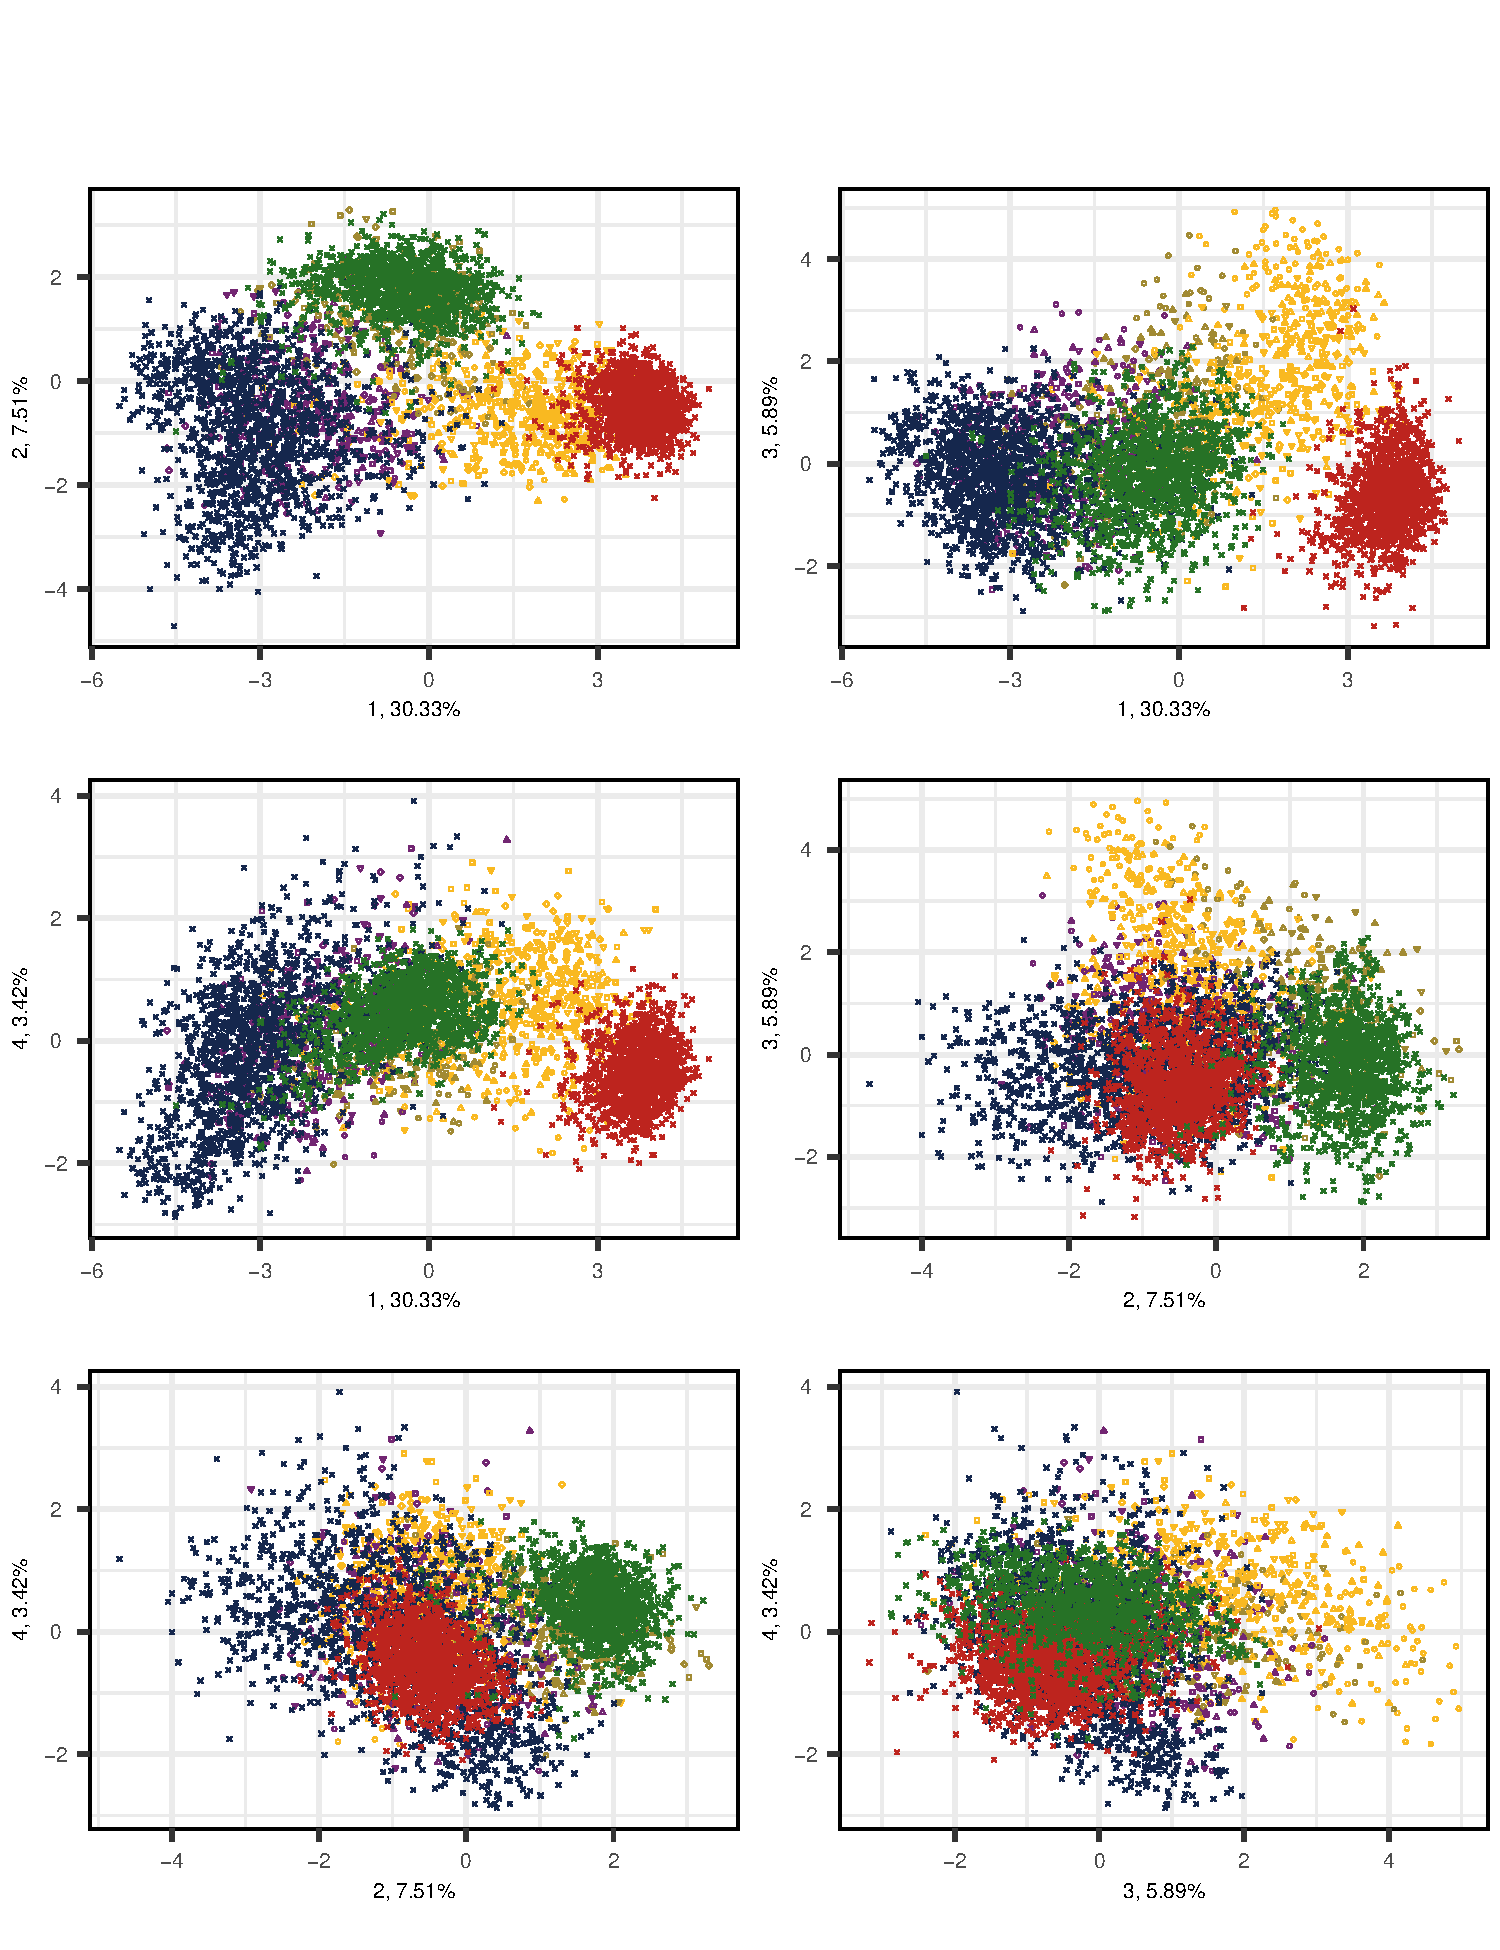
\includegraphics{G_Ch7_Analysis_files/figure-pdf/PCAtools-pairsplots-TxB-1.pdf}

\begin{Shaded}
\begin{Highlighting}[]
\CommentTok{\#dev.off()}
\CommentTok{\#ggsave(here("plots", "PCA\_TxB\_pairsplot.svg"), width = 6, height = 10)}
\CommentTok{\# Note that the legend has to be added manually (it was taken from the biplot code below).}
\end{Highlighting}
\end{Shaded}

\subsection{Bi-plots}\label{bi-plots-1}

Biplots are used to more closely examine the position of texts on just
two dimensions.

\begin{Shaded}
\begin{Highlighting}[]
\CommentTok{\# These settings (with legendPosition = "top") were used to generate the legend for the scatterplot matrix above:}
\CommentTok{\#png(here("plots", "PCA\_3Ref\_Biplot\_PC1\_PC2test.png"), width = 40, height= 25, units = "cm", res = 300) }

\NormalTok{PCAtools}\SpecialCharTok{::}\FunctionTok{biplot}\NormalTok{(p,}
                 \AttributeTok{x =} \StringTok{"PC1"}\NormalTok{,}
                 \AttributeTok{y =} \StringTok{"PC2"}\NormalTok{,}
                 \AttributeTok{lab =} \ConstantTok{NULL}\NormalTok{, }\CommentTok{\# Otherwise will try to label each data point!}
                 \AttributeTok{colby =} \StringTok{"Corpus"}\NormalTok{,}
                 \AttributeTok{pointSize =} \FloatTok{1.3}\NormalTok{,}
                 \AttributeTok{colkey =}\NormalTok{ colkey,}
                 \AttributeTok{shape =} \StringTok{"Level"}\NormalTok{,}
                 \AttributeTok{shapekey =}\NormalTok{ shapekey,}
                 \AttributeTok{xlim =} \FunctionTok{c}\NormalTok{(}\FunctionTok{min}\NormalTok{(p}\SpecialCharTok{$}\NormalTok{rotated[, }\StringTok{"PC1"}\NormalTok{]), }\FunctionTok{max}\NormalTok{(p}\SpecialCharTok{$}\NormalTok{rotated[, }\StringTok{"PC1"}\NormalTok{])),}
                 \AttributeTok{ylim =} \FunctionTok{c}\NormalTok{(}\FunctionTok{min}\NormalTok{(p}\SpecialCharTok{$}\NormalTok{rotated[, }\StringTok{"PC2"}\NormalTok{]), }\FunctionTok{max}\NormalTok{(p}\SpecialCharTok{$}\NormalTok{rotated[, }\StringTok{"PC2"}\NormalTok{])),}
                 \AttributeTok{showLoadings =} \ConstantTok{FALSE}\NormalTok{,}
                 \AttributeTok{ellipse =} \ConstantTok{TRUE}\NormalTok{,}
                 \AttributeTok{axisLabSize =} \DecValTok{18}\NormalTok{,}
                 \AttributeTok{legendPosition =} \StringTok{\textquotesingle{}right\textquotesingle{}}\NormalTok{,}
                 \AttributeTok{legendTitleSize =} \DecValTok{18}\NormalTok{,}
                 \AttributeTok{legendLabSize =} \DecValTok{14}\NormalTok{, }
                 \AttributeTok{legendIconSize =} \DecValTok{5}\NormalTok{) }\SpecialCharTok{+}
  \FunctionTok{theme}\NormalTok{(}\AttributeTok{plot.margin =} \FunctionTok{unit}\NormalTok{(}\FunctionTok{c}\NormalTok{(}\DecValTok{0}\NormalTok{,}\DecValTok{0}\NormalTok{,}\DecValTok{0}\NormalTok{,}\FloatTok{0.2}\NormalTok{), }\StringTok{"cm"}\NormalTok{))}
\end{Highlighting}
\end{Shaded}

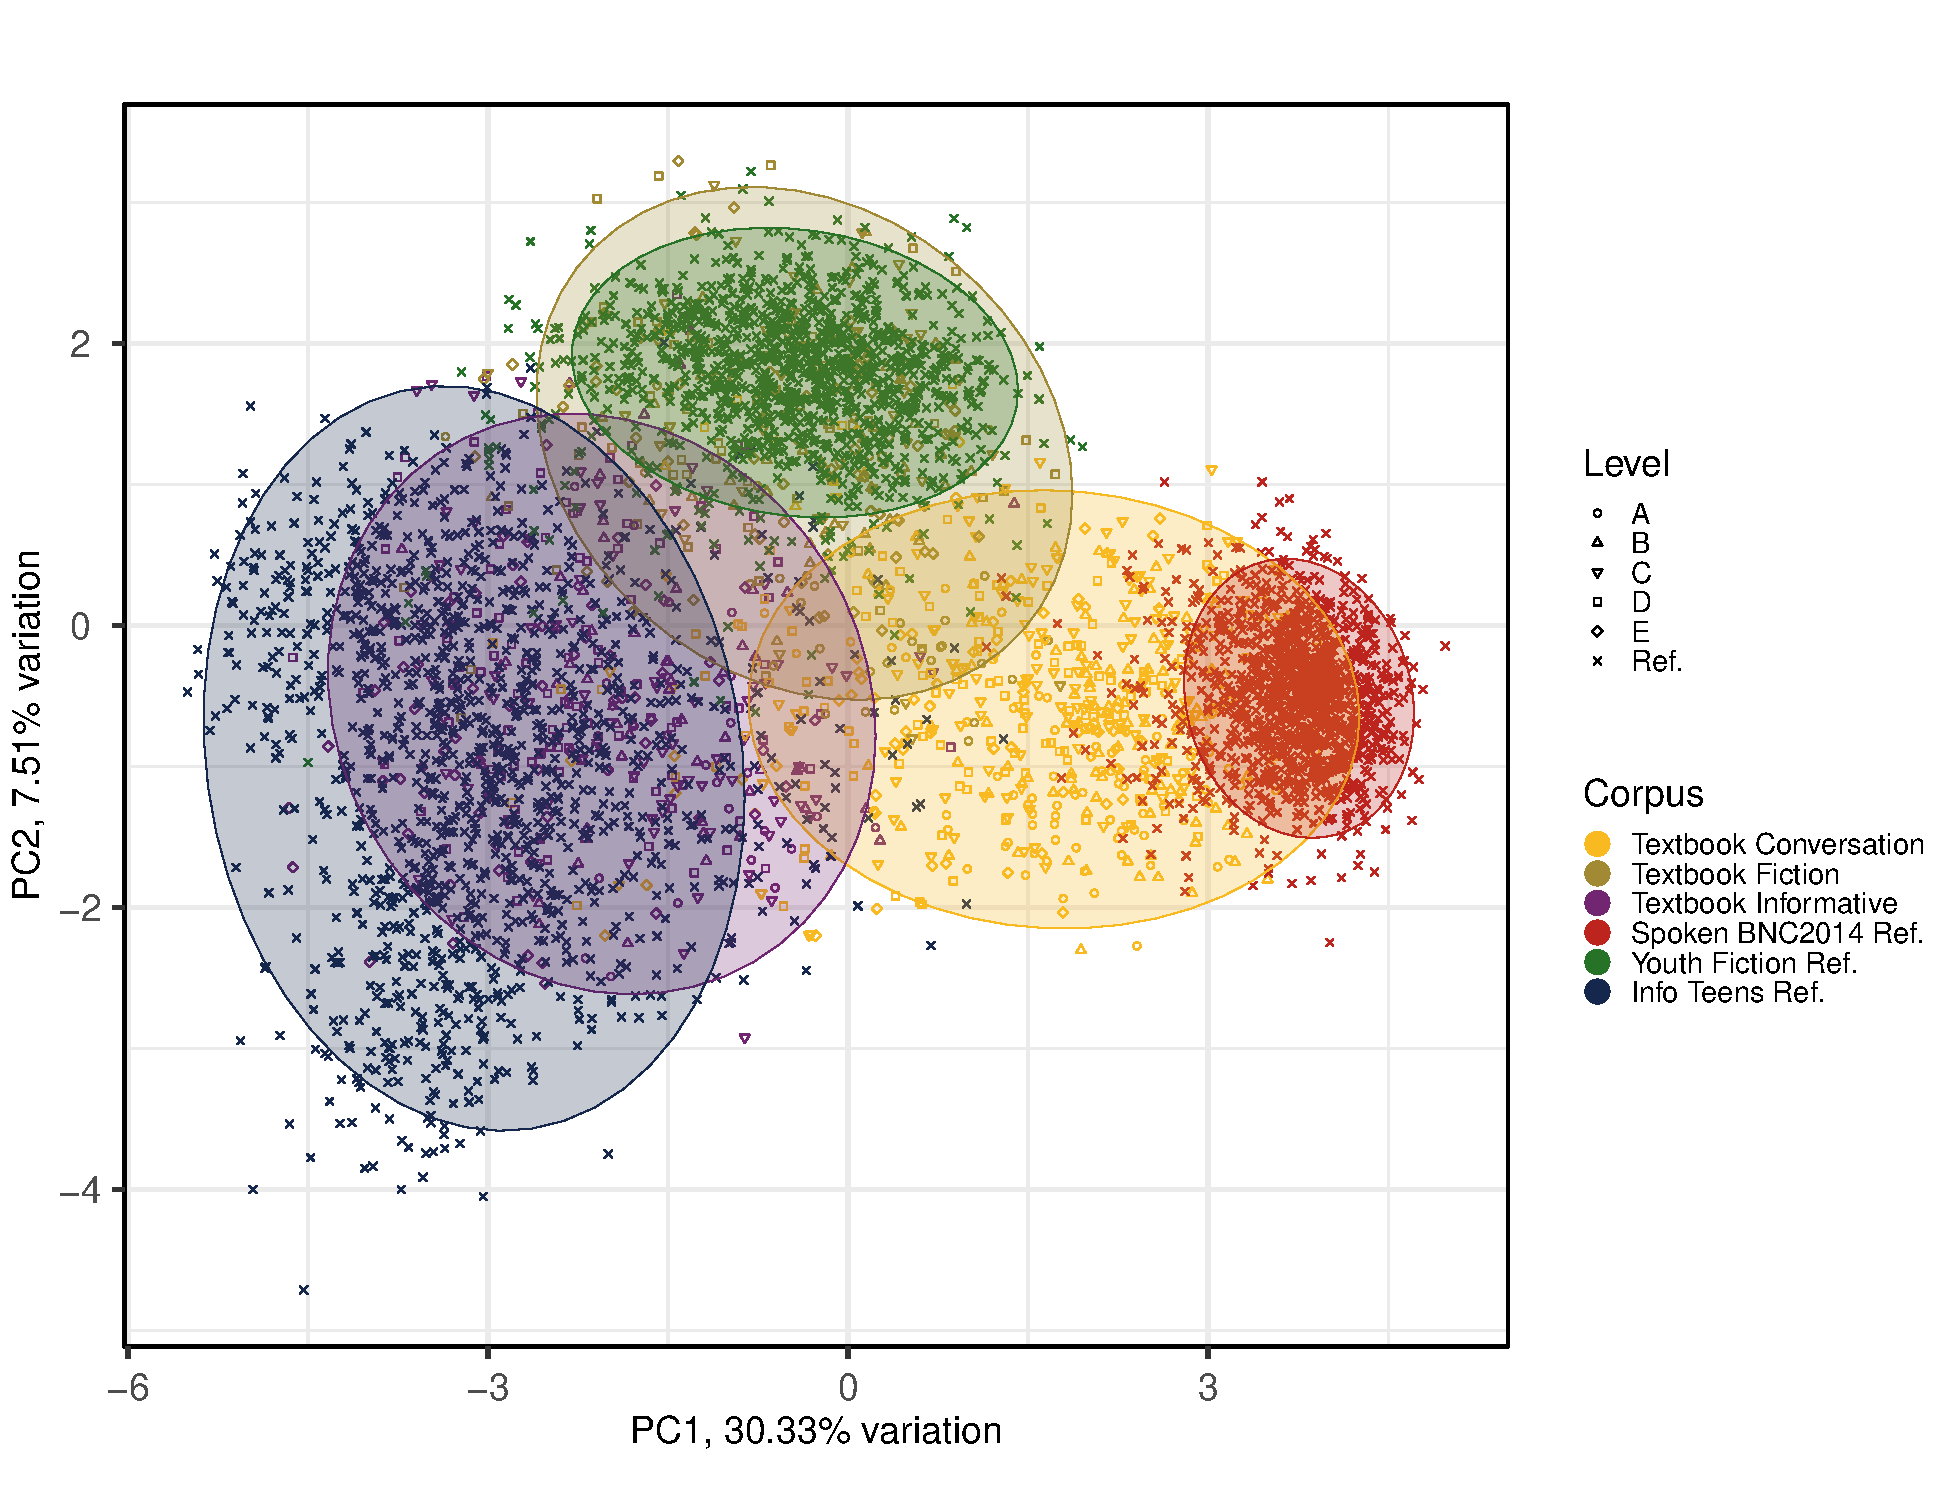
\includegraphics{G_Ch7_Analysis_files/figure-pdf/PCAtools-biplots-TxB-1.pdf}

\begin{Shaded}
\begin{Highlighting}[]
\CommentTok{\#ggsave(here("plots", "PCA\_Ref3TxB\_BiplotPC1\_PC2.svg"), width = 12, height = 8)}

\CommentTok{\# Biplots to examine components more carefully}
\NormalTok{PCAtools}\SpecialCharTok{::}\FunctionTok{biplot}\NormalTok{(p,}
                 \AttributeTok{x =} \StringTok{"PC3"}\NormalTok{,}
                 \AttributeTok{y =} \StringTok{"PC4"}\NormalTok{,}
                 \AttributeTok{lab =} \ConstantTok{NULL}\NormalTok{, }\CommentTok{\# Otherwise will try to label each data point!}
                 \AttributeTok{colby =} \StringTok{"Corpus"}\NormalTok{,}
                 \AttributeTok{pointSize =} \FloatTok{1.2}\NormalTok{,}
                 \AttributeTok{colkey =}\NormalTok{ colkey,}
                 \AttributeTok{shape =} \StringTok{"Level"}\NormalTok{,}
                 \AttributeTok{shapekey =}\NormalTok{ shapekey,}
                 \AttributeTok{xlim =} \FunctionTok{c}\NormalTok{(}\FunctionTok{min}\NormalTok{(p}\SpecialCharTok{$}\NormalTok{rotated[, }\StringTok{"PC3"}\NormalTok{]), }\FunctionTok{max}\NormalTok{(p}\SpecialCharTok{$}\NormalTok{rotated[, }\StringTok{"PC3"}\NormalTok{])),}
                 \AttributeTok{ylim =} \FunctionTok{c}\NormalTok{(}\FunctionTok{min}\NormalTok{(p}\SpecialCharTok{$}\NormalTok{rotated[, }\StringTok{"PC4"}\NormalTok{]), }\FunctionTok{max}\NormalTok{(p}\SpecialCharTok{$}\NormalTok{rotated[, }\StringTok{"PC4"}\NormalTok{])),}
                 \AttributeTok{showLoadings =} \ConstantTok{FALSE}\NormalTok{,}
                 \AttributeTok{ellipse =} \ConstantTok{TRUE}\NormalTok{,}
                 \AttributeTok{axisLabSize =} \DecValTok{18}\NormalTok{,}
                 \AttributeTok{legendPosition =} \StringTok{\textquotesingle{}right\textquotesingle{}}\NormalTok{,}
                 \AttributeTok{legendTitleSize =} \DecValTok{18}\NormalTok{,}
                 \AttributeTok{legendLabSize =} \DecValTok{14}\NormalTok{, }
                 \AttributeTok{legendIconSize =} \DecValTok{5}\NormalTok{) }\SpecialCharTok{+}
  \FunctionTok{theme}\NormalTok{(}\AttributeTok{plot.margin =} \FunctionTok{unit}\NormalTok{(}\FunctionTok{c}\NormalTok{(}\DecValTok{0}\NormalTok{,}\DecValTok{0}\NormalTok{,}\DecValTok{0}\NormalTok{,}\FloatTok{0.2}\NormalTok{), }\StringTok{"cm"}\NormalTok{))}
\end{Highlighting}
\end{Shaded}

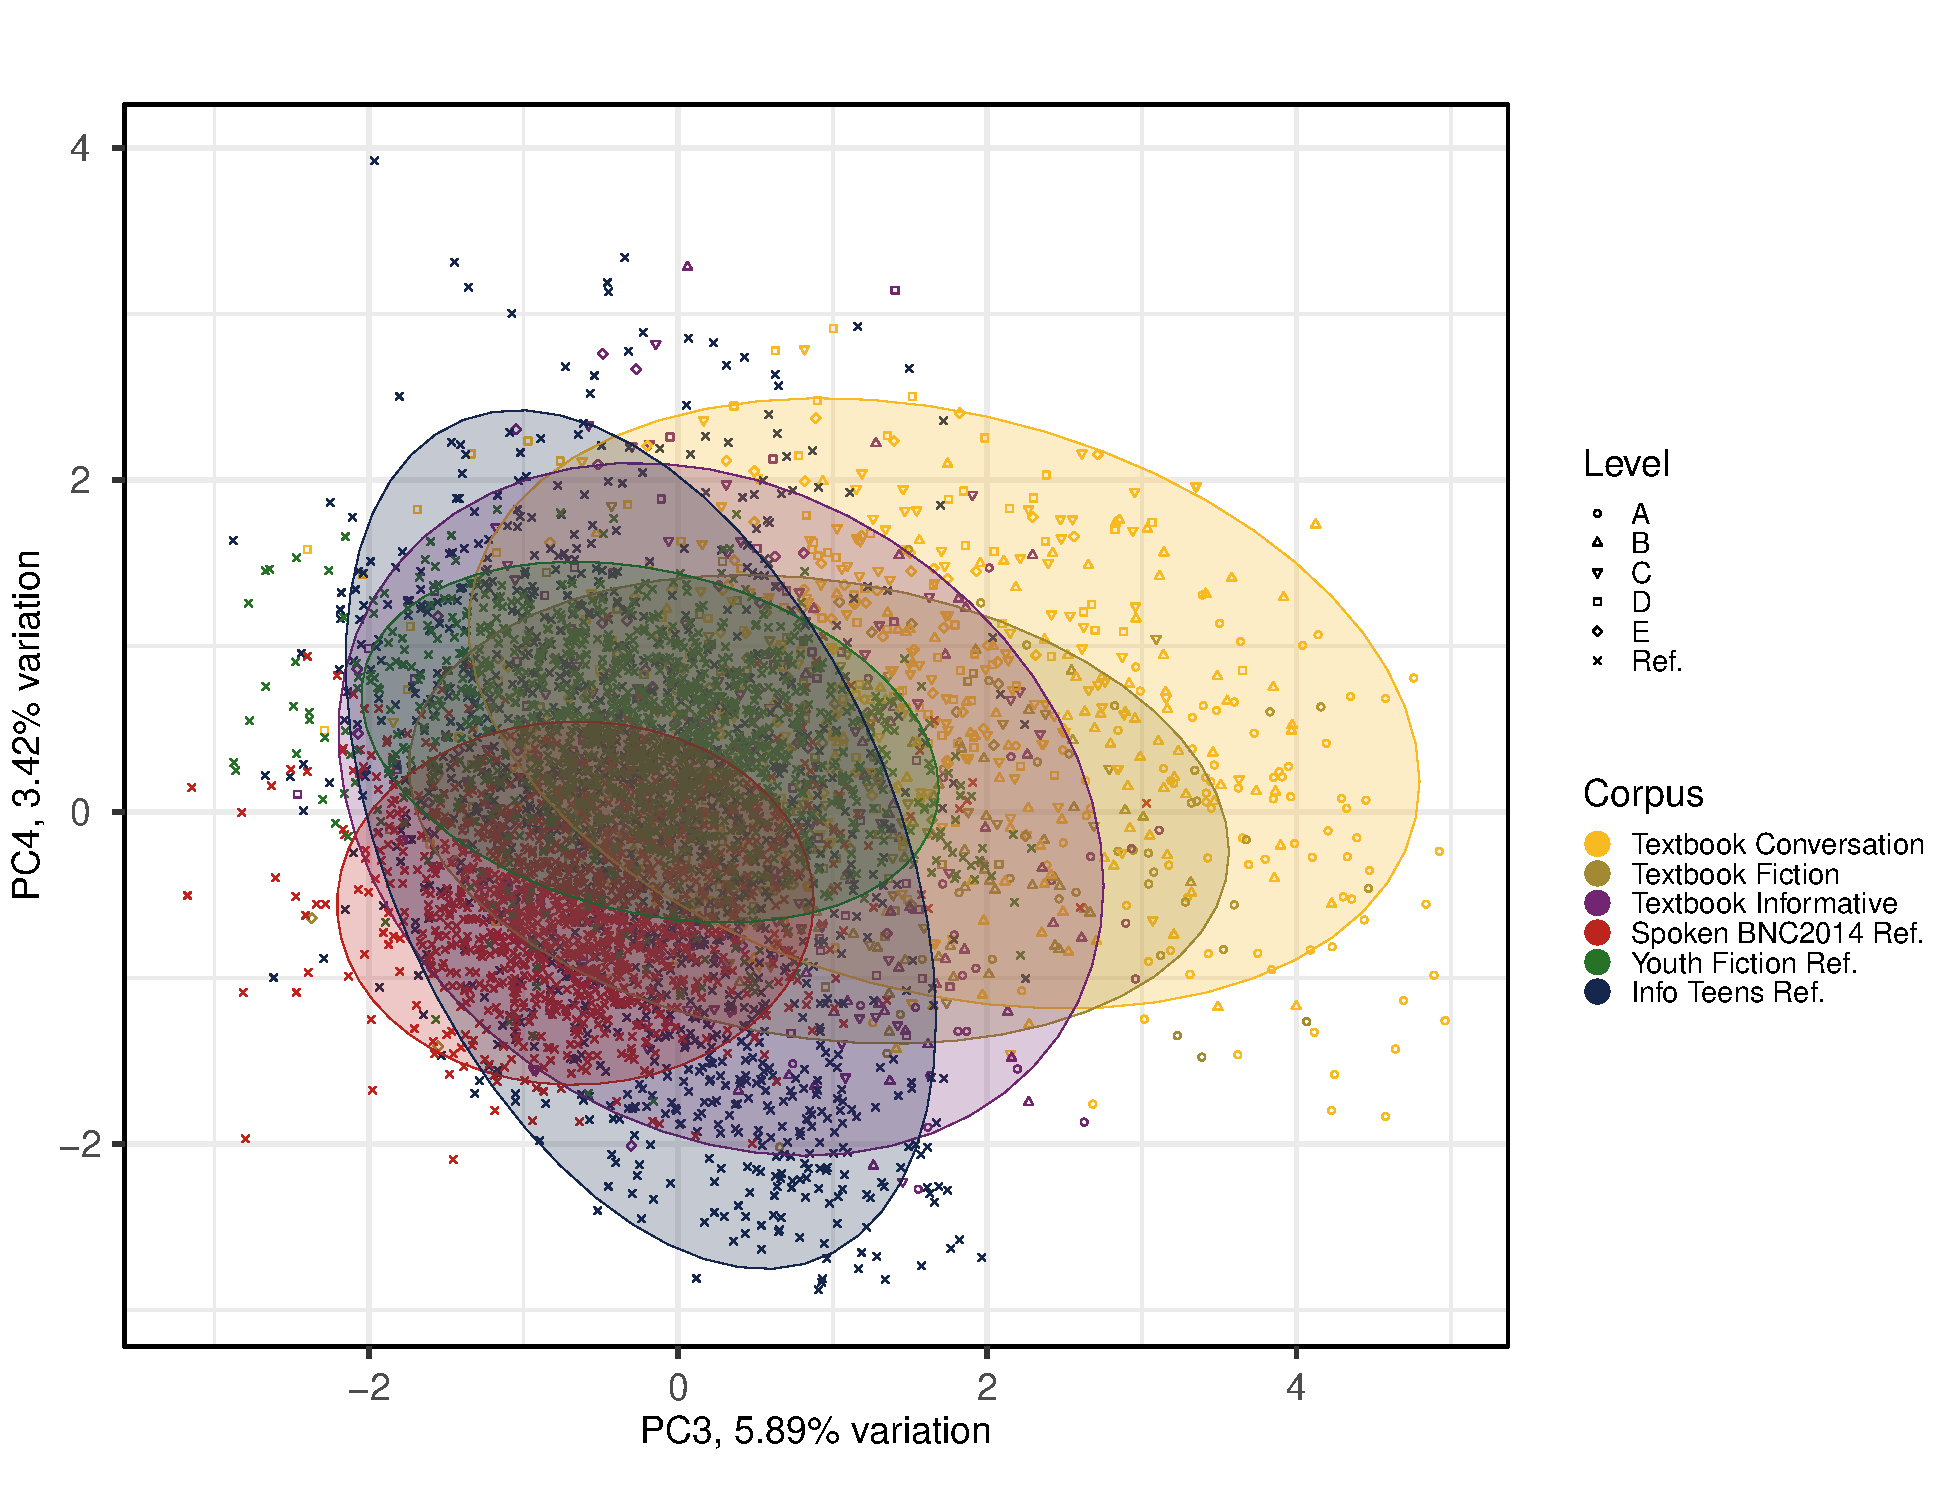
\includegraphics{G_Ch7_Analysis_files/figure-pdf/PCAtools-biplots-TxB-2.pdf}

\begin{Shaded}
\begin{Highlighting}[]
\CommentTok{\#ggsave(here("plots", "PCA\_Ref3TxB\_BiplotPC3\_PC4.svg"), width = 12, height = 8)}
\end{Highlighting}
\end{Shaded}

The colours and corresponding ellipses can be used to visualise
different clusters and patterns. In the following, we change the colour
of the points and the ellipses to represent the texts' target
proficiency levels instead of the register, allowing for a different
interpretation of the model.

\begin{Shaded}
\begin{Highlighting}[]
\CommentTok{\# Biplot with ellipses for Level rather than Register}
\NormalTok{colkeyLevels }\OtherTok{=} \FunctionTok{c}\NormalTok{(}\AttributeTok{A=}\StringTok{"\#F9B921"}\NormalTok{, }\AttributeTok{B=}\StringTok{"\#A18A33"}\NormalTok{, }\AttributeTok{C=}\StringTok{"\#BD241E"}\NormalTok{, }\AttributeTok{D=}\StringTok{"\#722672"}\NormalTok{, }\AttributeTok{E=}\StringTok{"\#15274D"}\NormalTok{, }\StringTok{\textasciigrave{}}\AttributeTok{Ref. data}\StringTok{\textasciigrave{}}\OtherTok{=} \StringTok{"darkgrey"}\NormalTok{)}
\NormalTok{shapekeyLevels }\OtherTok{=} \FunctionTok{c}\NormalTok{(}\StringTok{\textasciigrave{}}\AttributeTok{Spoken BNC2014 Ref.}\StringTok{\textasciigrave{}}\OtherTok{=}\DecValTok{16}\NormalTok{, }\StringTok{\textasciigrave{}}\AttributeTok{Info Teens Ref.}\StringTok{\textasciigrave{}}\OtherTok{=}\DecValTok{17}\NormalTok{, }\StringTok{\textasciigrave{}}\AttributeTok{Youth Fiction Ref.}\StringTok{\textasciigrave{}}\OtherTok{=}\DecValTok{15}\NormalTok{, }\StringTok{\textasciigrave{}}\AttributeTok{Textbook Fiction}\StringTok{\textasciigrave{}}\OtherTok{=}\DecValTok{0}\NormalTok{, }\StringTok{\textasciigrave{}}\AttributeTok{Textbook Conversation}\StringTok{\textasciigrave{}}\OtherTok{=}\DecValTok{1}\NormalTok{, }\StringTok{\textasciigrave{}}\AttributeTok{Textbook Informative}\StringTok{\textasciigrave{}}\OtherTok{=}\DecValTok{2}\NormalTok{)}

\NormalTok{PCAtools}\SpecialCharTok{::}\FunctionTok{biplot}\NormalTok{(p,}
                 \AttributeTok{x =} \StringTok{"PC3"}\NormalTok{,}
                 \AttributeTok{y =} \StringTok{"PC4"}\NormalTok{,}
                 \AttributeTok{lab =} \ConstantTok{NULL}\NormalTok{, }\CommentTok{\# Otherwise will try to label each data point!}
                 \AttributeTok{colby =} \StringTok{"Level"}\NormalTok{,}
                 \AttributeTok{pointSize =} \FloatTok{1.3}\NormalTok{,}
                 \AttributeTok{colkey =}\NormalTok{ colkeyLevels,}
                 \AttributeTok{shape =} \StringTok{"Corpus"}\NormalTok{,}
                 \AttributeTok{shapekey =}\NormalTok{ shapekeyLevels,}
                 \AttributeTok{xlim =} \FunctionTok{c}\NormalTok{(}\FunctionTok{min}\NormalTok{(p}\SpecialCharTok{$}\NormalTok{rotated[, }\StringTok{"PC3"}\NormalTok{]), }\FunctionTok{max}\NormalTok{(p}\SpecialCharTok{$}\NormalTok{rotated[, }\StringTok{"PC3"}\NormalTok{])),}
                 \AttributeTok{ylim =} \FunctionTok{c}\NormalTok{(}\FunctionTok{min}\NormalTok{(p}\SpecialCharTok{$}\NormalTok{rotated[, }\StringTok{"PC4"}\NormalTok{]), }\FunctionTok{max}\NormalTok{(p}\SpecialCharTok{$}\NormalTok{rotated[, }\StringTok{"PC4"}\NormalTok{])),}
                 \AttributeTok{showLoadings =} \ConstantTok{FALSE}\NormalTok{,}
                 \AttributeTok{ellipse =} \ConstantTok{TRUE}\NormalTok{,}
                 \AttributeTok{axisLabSize =} \DecValTok{18}\NormalTok{,}
                 \AttributeTok{legendPosition =} \StringTok{\textquotesingle{}right\textquotesingle{}}\NormalTok{,}
                 \AttributeTok{legendTitleSize =} \DecValTok{18}\NormalTok{,}
                 \AttributeTok{legendLabSize =} \DecValTok{14}\NormalTok{, }
                 \AttributeTok{legendIconSize =} \DecValTok{5}\NormalTok{) }\SpecialCharTok{+}
  \FunctionTok{theme}\NormalTok{(}\AttributeTok{plot.margin =} \FunctionTok{unit}\NormalTok{(}\FunctionTok{c}\NormalTok{(}\DecValTok{0}\NormalTok{,}\DecValTok{0}\NormalTok{,}\DecValTok{0}\NormalTok{,}\FloatTok{0.2}\NormalTok{), }\StringTok{"cm"}\NormalTok{))}
\end{Highlighting}
\end{Shaded}

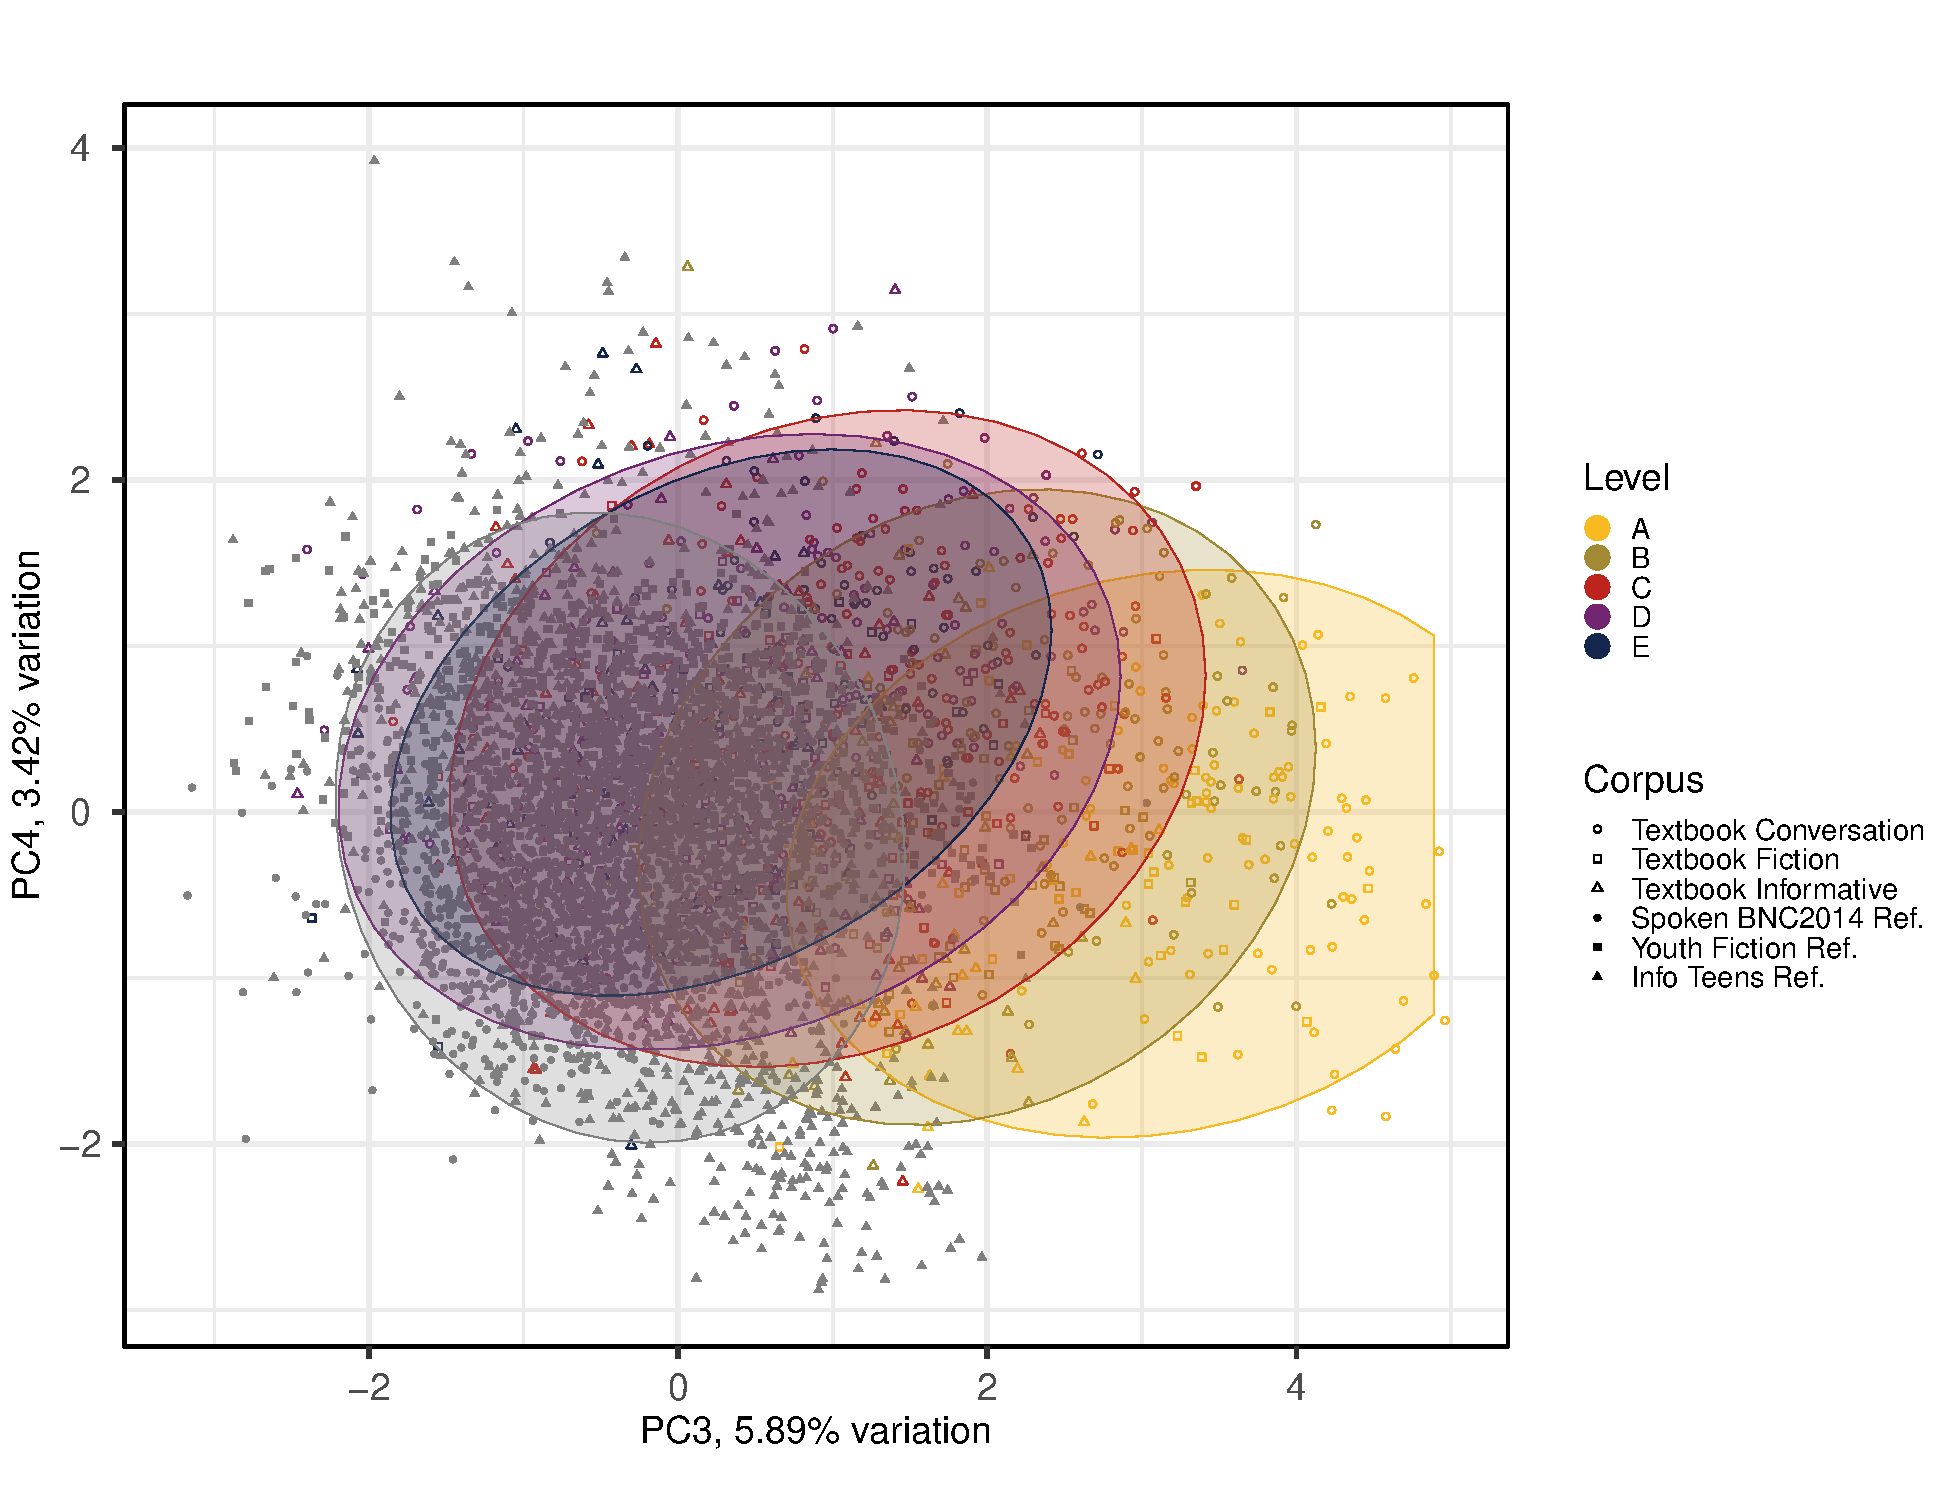
\includegraphics{G_Ch7_Analysis_files/figure-pdf/PCAtools-biplots-TxB-Levels-1.pdf}

\begin{Shaded}
\begin{Highlighting}[]
\CommentTok{\#ggsave(here("plots", "PCA\_Ref3TxB\_BiplotPC3\_PC4\_levels.svg"), width = 12, height = 8)}
\end{Highlighting}
\end{Shaded}

\section{Feature contributions (loadings) on each
component}\label{feature-contributions-loadings-on-each-component-1}

\begin{Shaded}
\begin{Highlighting}[]
\CommentTok{\#data \textless{}{-} readRDS(here("processed\_data", "dataforPCA.rds")) }
\NormalTok{pca }\OtherTok{\textless{}{-}} \FunctionTok{prcomp}\NormalTok{(data[,}\DecValTok{9}\SpecialCharTok{:}\FunctionTok{ncol}\NormalTok{(data)], }\AttributeTok{scale.=}\ConstantTok{FALSE}\NormalTok{) }\CommentTok{\# All quantitative variables to be included in the model}

\CommentTok{\# The rotated data that represents the observations / samples is stored in rotated, while the variable loadings are stored in loadings}
\NormalTok{loadings }\OtherTok{\textless{}{-}} \FunctionTok{as.data.frame}\NormalTok{(pca}\SpecialCharTok{$}\NormalTok{rotation[,}\DecValTok{1}\SpecialCharTok{:}\DecValTok{4}\NormalTok{])}

\CommentTok{\# Table of loadings with no minimum threshold applied}
\NormalTok{loadings }\SpecialCharTok{|\textgreater{}} 
  \FunctionTok{round}\NormalTok{(}\DecValTok{2}\NormalTok{) }\SpecialCharTok{|\textgreater{}} 
  \FunctionTok{kable}\NormalTok{()}
\end{Highlighting}
\end{Shaded}

\begin{longtable}[]{@{}lrrrr@{}}
\toprule\noalign{}
& PC1 & PC2 & PC3 & PC4 \\
\midrule\noalign{}
\endhead
\bottomrule\noalign{}
\endlastfoot
ACT & -0.10 & 0.01 & -0.01 & 0.12 \\
AMP & 0.00 & -0.05 & -0.05 & 0.09 \\
ASPECT & -0.08 & 0.10 & -0.01 & 0.00 \\
AWL & -0.21 & -0.13 & -0.06 & -0.01 \\
BEMA & 0.08 & -0.24 & 0.06 & -0.02 \\
CAUSE & -0.08 & -0.12 & 0.06 & 0.14 \\
CC & -0.14 & -0.13 & -0.09 & -0.09 \\
COMM & -0.03 & 0.19 & 0.03 & 0.20 \\
CONC & -0.03 & -0.03 & -0.18 & -0.06 \\
COND & 0.08 & -0.02 & -0.17 & 0.23 \\
CONT & 0.22 & -0.05 & 0.03 & 0.00 \\
CUZ & 0.10 & -0.14 & -0.20 & -0.18 \\
DEMO & 0.15 & -0.12 & -0.08 & -0.04 \\
DMA & 0.20 & -0.09 & -0.04 & -0.16 \\
DOAUX & 0.18 & -0.02 & 0.06 & 0.00 \\
DT & 0.08 & 0.16 & -0.24 & -0.03 \\
DWNT & -0.04 & 0.10 & -0.12 & 0.09 \\
ELAB & -0.07 & -0.17 & -0.04 & 0.07 \\
EMPH & 0.17 & -0.07 & -0.09 & -0.03 \\
EX & 0.06 & -0.02 & -0.04 & 0.00 \\
EXIST & -0.13 & -0.09 & -0.05 & 0.00 \\
FPP1P & 0.08 & -0.02 & 0.09 & 0.19 \\
FPP1S & 0.17 & 0.06 & 0.06 & 0.08 \\
FPUH & 0.18 & -0.10 & -0.05 & -0.19 \\
GTO & 0.14 & 0.00 & -0.04 & 0.00 \\
HDG & 0.10 & -0.07 & -0.14 & -0.12 \\
HGOT & 0.16 & -0.05 & -0.01 & -0.11 \\
IN & -0.21 & -0.01 & -0.08 & 0.01 \\
JJAT & -0.05 & -0.13 & -0.25 & 0.07 \\
JJPR & -0.03 & -0.17 & -0.03 & 0.21 \\
LD & -0.17 & -0.16 & 0.13 & -0.04 \\
MDCA & 0.05 & -0.21 & 0.11 & 0.22 \\
MDCO & 0.00 & 0.19 & -0.15 & 0.10 \\
MDMM & -0.02 & -0.10 & -0.14 & 0.17 \\
MDNE & 0.06 & -0.02 & -0.06 & 0.22 \\
MDWO & 0.07 & 0.11 & -0.18 & 0.04 \\
MDWS & 0.06 & -0.02 & -0.01 & 0.25 \\
MENTAL & 0.11 & -0.02 & -0.05 & 0.16 \\
NCOMP & 0.00 & -0.27 & -0.05 & 0.03 \\
NN & -0.21 & -0.10 & 0.10 & -0.07 \\
OCCUR & -0.13 & -0.02 & -0.05 & -0.06 \\
PASS & -0.14 & -0.13 & -0.09 & -0.10 \\
PEAS & -0.06 & 0.12 & -0.19 & 0.12 \\
PIT & 0.15 & -0.10 & -0.15 & -0.07 \\
PLACE & 0.02 & 0.09 & 0.09 & 0.07 \\
POLITE & 0.09 & 0.00 & 0.20 & 0.11 \\
POS & 0.02 & 0.09 & 0.04 & -0.05 \\
PROG & 0.09 & 0.08 & -0.04 & 0.15 \\
QUAN & 0.17 & -0.01 & -0.16 & 0.01 \\
QUPR & 0.08 & 0.11 & -0.12 & 0.21 \\
QUTAG & 0.15 & -0.04 & -0.07 & -0.15 \\
RB & 0.14 & 0.15 & -0.18 & 0.07 \\
RP & -0.01 & 0.22 & -0.09 & 0.15 \\
SPLIT & -0.03 & -0.11 & -0.21 & 0.08 \\
SPP2 & 0.17 & -0.07 & 0.10 & 0.16 \\
STPR & 0.10 & 0.01 & 0.01 & -0.04 \\
THATD & 0.16 & -0.01 & -0.14 & -0.02 \\
THRC & -0.05 & -0.17 & -0.15 & -0.02 \\
THSC & -0.02 & -0.08 & -0.27 & 0.07 \\
TTR & -0.19 & 0.07 & -0.02 & 0.16 \\
VBD & -0.10 & 0.35 & -0.05 & -0.20 \\
VBG & -0.14 & -0.02 & -0.14 & 0.12 \\
VBN & -0.14 & -0.10 & -0.08 & -0.07 \\
VIMP & 0.01 & -0.07 & 0.21 & 0.21 \\
WHQU & 0.13 & -0.02 & 0.20 & 0.07 \\
WHSC & -0.09 & -0.10 & -0.20 & 0.05 \\
XX0 & 0.18 & 0.01 & -0.06 & 0.06 \\
YNQU & 0.18 & -0.03 & 0.14 & -0.02 \\
TPP3 & -0.05 & 0.30 & -0.04 & -0.15 \\
FQTI & -0.07 & 0.03 & 0.01 & 0.14 \\
\end{longtable}

\begin{Shaded}
\begin{Highlighting}[]
\CommentTok{\#clipr::write\_last\_clip()}
\end{Highlighting}
\end{Shaded}

\section{Graphs of features of that contribute most to each
component/dimension}\label{graphs-of-features-of-that-contribute-most-to-each-componentdimension}

Graphs of features display the features with the strongest contributions
to any two dimensions of the model of intra-textbook variation. They are
created using the \texttt{factoextra::fviz\_pca\_var} function.

\begin{Shaded}
\begin{Highlighting}[]
\NormalTok{factoextra}\SpecialCharTok{::}\FunctionTok{fviz\_pca\_var}\NormalTok{(pca,}
             \AttributeTok{axes =} \FunctionTok{c}\NormalTok{(}\DecValTok{1}\NormalTok{,}\DecValTok{2}\NormalTok{),}
             \AttributeTok{select.var =} \FunctionTok{list}\NormalTok{(}\AttributeTok{contrib =} \DecValTok{25}\NormalTok{),}
             \AttributeTok{col.var =} \StringTok{"contrib"}\NormalTok{, }\CommentTok{\# Colour by contributions to the PC}
             \AttributeTok{gradient.cols =} \FunctionTok{c}\NormalTok{(}\StringTok{"\#F9B921"}\NormalTok{, }\StringTok{"\#DB241E"}\NormalTok{, }\StringTok{"\#722672"}\NormalTok{),}
             \AttributeTok{title =} \StringTok{""}\NormalTok{,}
             \AttributeTok{repel =} \ConstantTok{TRUE}\NormalTok{, }\CommentTok{\# Try to avoid too much text overlapping}
             \AttributeTok{ggtheme =}\NormalTok{ ggthemes}\SpecialCharTok{::}\FunctionTok{theme\_few}\NormalTok{())}
\end{Highlighting}
\end{Shaded}

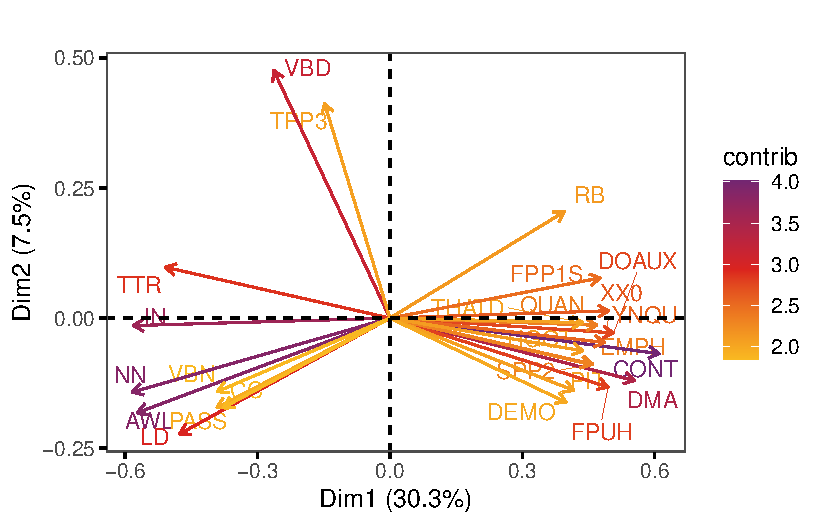
\includegraphics{G_Ch7_Analysis_files/figure-pdf/graphs-of-variables-1.pdf}

\begin{Shaded}
\begin{Highlighting}[]
\CommentTok{\#ggsave(here("plots", "fviz\_pca\_var\_PC1\_PC2\_Ref3Reg.svg"), width = 9, height = 7)}

\NormalTok{factoextra}\SpecialCharTok{::}\FunctionTok{fviz\_pca\_var}\NormalTok{(pca,}
             \AttributeTok{axes =} \FunctionTok{c}\NormalTok{(}\DecValTok{3}\NormalTok{,}\DecValTok{2}\NormalTok{),}
             \AttributeTok{select.var =} \FunctionTok{list}\NormalTok{(}\AttributeTok{contrib =} \DecValTok{30}\NormalTok{),}
             \AttributeTok{col.var =} \StringTok{"contrib"}\NormalTok{, }\CommentTok{\# Colour by contributions to the PC}
             \AttributeTok{gradient.cols =} \FunctionTok{c}\NormalTok{(}\StringTok{"\#F9B921"}\NormalTok{, }\StringTok{"\#DB241E"}\NormalTok{, }\StringTok{"\#722672"}\NormalTok{),}
             \AttributeTok{title =} \StringTok{""}\NormalTok{,}
             \AttributeTok{repel =} \ConstantTok{TRUE}\NormalTok{, }\CommentTok{\# Try to avoid too much text overlapping}
             \AttributeTok{ggtheme =}\NormalTok{ ggthemes}\SpecialCharTok{::}\FunctionTok{theme\_few}\NormalTok{())}
\end{Highlighting}
\end{Shaded}

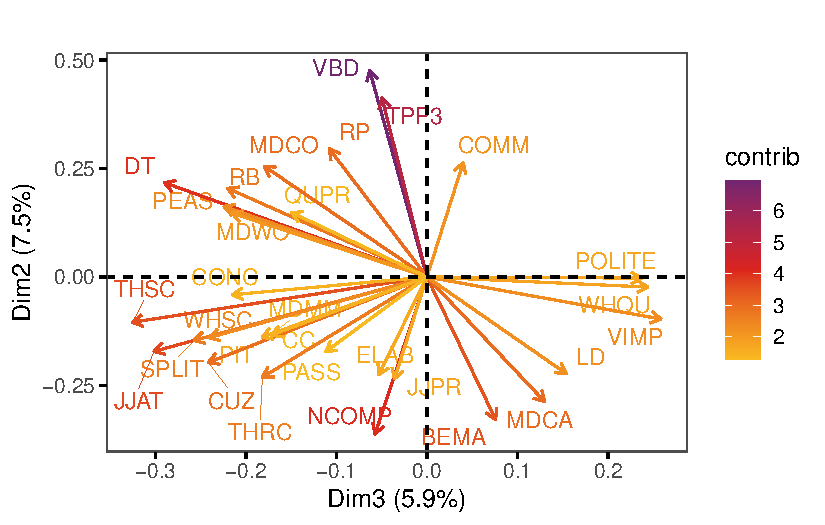
\includegraphics{G_Ch7_Analysis_files/figure-pdf/graphs-of-variables-2.pdf}

\begin{Shaded}
\begin{Highlighting}[]
\CommentTok{\#ggsave(here("plots", "fviz\_pca\_var\_PC3\_PC2\_Ref3Reg.svg"), width = 9, height = 8)}

\NormalTok{factoextra}\SpecialCharTok{::}\FunctionTok{fviz\_pca\_var}\NormalTok{(pca,}
             \AttributeTok{axes =} \FunctionTok{c}\NormalTok{(}\DecValTok{3}\NormalTok{,}\DecValTok{4}\NormalTok{),}
             \AttributeTok{select.var =} \FunctionTok{list}\NormalTok{(}\AttributeTok{contrib =} \DecValTok{30}\NormalTok{),}
             \AttributeTok{col.var =} \StringTok{"contrib"}\NormalTok{, }\CommentTok{\# Colour by contributions to the PC}
             \AttributeTok{gradient.cols =} \FunctionTok{c}\NormalTok{(}\StringTok{"\#F9B921"}\NormalTok{, }\StringTok{"\#DB241E"}\NormalTok{, }\StringTok{"\#722672"}\NormalTok{),}
             \AttributeTok{title =} \StringTok{""}\NormalTok{,}
             \AttributeTok{repel =} \ConstantTok{TRUE}\NormalTok{, }\CommentTok{\# Try to avoid too much text overlapping}
             \AttributeTok{ggtheme =}\NormalTok{ ggthemes}\SpecialCharTok{::}\FunctionTok{theme\_few}\NormalTok{())}
\end{Highlighting}
\end{Shaded}

\includegraphics{G_Ch7_Analysis_files/figure-pdf/graphs-of-variables-3.pdf}

\begin{Shaded}
\begin{Highlighting}[]
\CommentTok{\#ggsave(here("plots", "fviz\_pca\_var\_PC3\_PC4\_Ref3Reg.svg"), width = 9, height = 8)}
\end{Highlighting}
\end{Shaded}

\section{Exploring feature contributions in terms of normalised
frequencies}\label{exploring-feature-contributions-in-terms-of-normalised-frequencies}

We can go back to the normalised frequencies of the individual features
to compare them across different registers and levels, e.g.,:

\begin{Shaded}
\begin{Highlighting}[]
\NormalTok{ncounts }\OtherTok{\textless{}{-}} \FunctionTok{readRDS}\NormalTok{(}\FunctionTok{here}\NormalTok{(}\StringTok{"data"}\NormalTok{, }\StringTok{"processed"}\NormalTok{, }\StringTok{"ncounts3\_3Reg.rds"}\NormalTok{))}

\NormalTok{ncounts }\SpecialCharTok{|\textgreater{}} 
  \FunctionTok{filter}\NormalTok{(Register}\SpecialCharTok{==}\StringTok{"Informative"}\NormalTok{) }\SpecialCharTok{|\textgreater{}} 
  \CommentTok{\#filter(Level \%in\% c("C", "D", "E")) |\textgreater{} }
  \FunctionTok{select}\NormalTok{(Level, VBD, PEAS) }\SpecialCharTok{|\textgreater{}} 
  \FunctionTok{group\_by}\NormalTok{(Level) }\SpecialCharTok{|\textgreater{}} 
  \FunctionTok{summarise\_if}\NormalTok{(is.numeric, mean) }\SpecialCharTok{|\textgreater{}} 
  \FunctionTok{kable}\NormalTok{(}\AttributeTok{digits=}\DecValTok{2}\NormalTok{)}
\end{Highlighting}
\end{Shaded}

\begin{longtable}[]{@{}lrr@{}}
\toprule\noalign{}
Level & VBD & PEAS \\
\midrule\noalign{}
\endhead
\bottomrule\noalign{}
\endlastfoot
A & 28.11 & 0.21 \\
B & 34.11 & 2.49 \\
C & 35.21 & 5.36 \\
D & 39.83 & 7.63 \\
E & 35.17 & 6.91 \\
Ref. & 39.73 & 4.94 \\
\end{longtable}

The following chunk produces Figure 35 which shows normalised counts of
selected features with salient loadings on PC1 in the Textbook
Informative subcorpus (Levels A to E) and the reference Info Teens
corpus (Ref.). This plots visualises the observed normalised frequencies
as they were extracted using the MFTE Perl (see Appendices C and F).

\begin{Shaded}
\begin{Highlighting}[]
\NormalTok{cols }\OtherTok{=} \FunctionTok{c}\NormalTok{(}\StringTok{"\#F9B921"}\NormalTok{, }\StringTok{"\#A18A33"}\NormalTok{, }\StringTok{"\#BD241E"}\NormalTok{, }\StringTok{"\#722672"}\NormalTok{, }\StringTok{"\#15274D"}\NormalTok{, }\StringTok{"darkgrey"}\NormalTok{)}

\NormalTok{boxfeature }\OtherTok{\textless{}{-}}\NormalTok{ ncounts }\SpecialCharTok{|\textgreater{}} 
  \FunctionTok{filter}\NormalTok{(Register}\SpecialCharTok{==}\StringTok{"Informative"}\NormalTok{) }\SpecialCharTok{|\textgreater{}} 
  \CommentTok{\#filter(Level \%in\% c("C", "D", "E")) |\textgreater{} }
  \FunctionTok{select}\NormalTok{(Level, FPP1S, SPP2, CONT, EXIST, AWL, XX0, PASS, VBN) }\SpecialCharTok{|\textgreater{}} 
  \FunctionTok{ggplot}\NormalTok{(}\FunctionTok{aes}\NormalTok{(}\AttributeTok{x =}\NormalTok{ Level, }\AttributeTok{y =}\NormalTok{ CONT, }\AttributeTok{colour =}\NormalTok{ Level, }\AttributeTok{fill =}\NormalTok{ Level)) }\SpecialCharTok{+}
  \FunctionTok{geom\_jitter}\NormalTok{(}\AttributeTok{size=}\FloatTok{0.7}\NormalTok{, }\AttributeTok{alpha=}\NormalTok{.}\DecValTok{7}\NormalTok{) }\SpecialCharTok{+}
  \FunctionTok{geom\_boxplot}\NormalTok{(}\AttributeTok{outlier.shape =} \ConstantTok{NA}\NormalTok{, }\AttributeTok{fatten =} \DecValTok{2}\NormalTok{, }\AttributeTok{fill =} \StringTok{"white"}\NormalTok{, }\AttributeTok{alpha =} \FloatTok{0.3}\NormalTok{) }\SpecialCharTok{+}
  \FunctionTok{scale\_colour\_manual}\NormalTok{(}\AttributeTok{values =}\NormalTok{ cols) }\SpecialCharTok{+}
  \FunctionTok{theme\_minimal}\NormalTok{() }\SpecialCharTok{+}
  \FunctionTok{theme}\NormalTok{(}\AttributeTok{legend.position =} \StringTok{"none"}\NormalTok{) }\SpecialCharTok{+}
  \FunctionTok{xlab}\NormalTok{(}\StringTok{""}\NormalTok{)}

\NormalTok{CONT }\OtherTok{=}\NormalTok{ boxfeature}
\NormalTok{SPP2 }\OtherTok{\textless{}{-}}\NormalTok{ boxfeature }\SpecialCharTok{+} \FunctionTok{aes}\NormalTok{(}\AttributeTok{y =}\NormalTok{ SPP2) }
\NormalTok{EXIST }\OtherTok{\textless{}{-}}\NormalTok{ boxfeature }\SpecialCharTok{+} \FunctionTok{aes}\NormalTok{(}\AttributeTok{y =}\NormalTok{ EXIST) }\SpecialCharTok{+} \FunctionTok{ylim}\NormalTok{(}\FunctionTok{c}\NormalTok{(}\DecValTok{0}\NormalTok{,}\DecValTok{25}\NormalTok{)) }\CommentTok{\# These y{-}axis limits remove individual outliers that overextend the scales and make the existing differences invisible to the naked eye. They can be removed to visualise all data points.}
\NormalTok{FFP1 }\OtherTok{\textless{}{-}}\NormalTok{ boxfeature }\SpecialCharTok{+} \FunctionTok{aes}\NormalTok{(}\AttributeTok{y =}\NormalTok{ FPP1S) }\SpecialCharTok{+} \FunctionTok{ylim}\NormalTok{(}\FunctionTok{c}\NormalTok{(}\DecValTok{0}\NormalTok{,}\DecValTok{60}\NormalTok{))  }
\NormalTok{AWL }\OtherTok{\textless{}{-}}\NormalTok{ boxfeature }\SpecialCharTok{+} \FunctionTok{aes}\NormalTok{(}\AttributeTok{y =}\NormalTok{ AWL)}
\NormalTok{XX0 }\OtherTok{\textless{}{-}}\NormalTok{ boxfeature }\SpecialCharTok{+} \FunctionTok{aes}\NormalTok{(}\AttributeTok{y =}\NormalTok{ XX0) }\SpecialCharTok{+} \FunctionTok{ylim}\NormalTok{(}\FunctionTok{c}\NormalTok{(}\DecValTok{0}\NormalTok{,}\DecValTok{25}\NormalTok{))}
\NormalTok{PASS }\OtherTok{\textless{}{-}}\NormalTok{ boxfeature }\SpecialCharTok{+} \FunctionTok{aes}\NormalTok{(}\AttributeTok{y =}\NormalTok{ PASS)}
\NormalTok{VBN }\OtherTok{\textless{}{-}}\NormalTok{ boxfeature }\SpecialCharTok{+} \FunctionTok{aes}\NormalTok{(}\AttributeTok{y =}\NormalTok{ VBN) }\SpecialCharTok{+} \FunctionTok{ylim}\NormalTok{(}\FunctionTok{c}\NormalTok{(}\DecValTok{0}\NormalTok{,}\DecValTok{40}\NormalTok{))}

\NormalTok{boxplots }\OtherTok{\textless{}{-}}\NormalTok{ gridExtra}\SpecialCharTok{::}\FunctionTok{grid.arrange}\NormalTok{(PASS, VBN, AWL, EXIST, FFP1, SPP2, CONT, XX0, }\AttributeTok{ncol=}\DecValTok{2}\NormalTok{, }\AttributeTok{nrow=}\DecValTok{4}\NormalTok{)}
\end{Highlighting}
\end{Shaded}

\includegraphics{G_Ch7_Analysis_files/figure-pdf/boxplots-1.pdf}

\begin{Shaded}
\begin{Highlighting}[]
\CommentTok{\#ggsave(here("plots", "BoxplotsInformativeFeatures.svg"), plot = boxplots, dpi = 300, width = 9, height = 11)}
\end{Highlighting}
\end{Shaded}

\section{Exploring the dimensions of the
model}\label{exploring-the-dimensions-of-the-model-1}

We begin with some descriptive statistics of the dimension scores.

\begin{Shaded}
\begin{Highlighting}[]
\CommentTok{\#data \textless{}{-} readRDS(here("data", "processed", "dataforPCA.rds")) }
\CommentTok{\#colnames(data)}
\NormalTok{pca }\OtherTok{\textless{}{-}} \FunctionTok{prcomp}\NormalTok{(data[,}\DecValTok{9}\SpecialCharTok{:}\FunctionTok{ncol}\NormalTok{(data)], }\AttributeTok{scale.=}\ConstantTok{FALSE}\NormalTok{) }\CommentTok{\# All quantitative variables}

\DocumentationTok{\#\# Access to the PCA results}
\CommentTok{\#colnames(data)}
\NormalTok{res.ind }\OtherTok{\textless{}{-}} \FunctionTok{cbind}\NormalTok{(data[,}\DecValTok{1}\SpecialCharTok{:}\DecValTok{8}\NormalTok{], }\FunctionTok{as.data.frame}\NormalTok{(pca}\SpecialCharTok{$}\NormalTok{x)[,}\DecValTok{1}\SpecialCharTok{:}\DecValTok{4}\NormalTok{])}

\DocumentationTok{\#\# Summary statistics}
\NormalTok{res.ind }\SpecialCharTok{|\textgreater{}} 
  \FunctionTok{group\_by}\NormalTok{(Subcorpus, Level) }\SpecialCharTok{|\textgreater{}} 
  \FunctionTok{summarise\_if}\NormalTok{(is.numeric, }\FunctionTok{c}\NormalTok{(}\AttributeTok{mean =}\NormalTok{ mean, }\AttributeTok{sd =}\NormalTok{ sd)) }\SpecialCharTok{|\textgreater{}} 
  \FunctionTok{kable}\NormalTok{(}\AttributeTok{digits =} \DecValTok{2}\NormalTok{)  }
\end{Highlighting}
\end{Shaded}

\begin{longtable}[]{@{}
  >{\raggedright\arraybackslash}p{(\columnwidth - 22\tabcolsep) * \real{0.1964}}
  >{\raggedright\arraybackslash}p{(\columnwidth - 22\tabcolsep) * \real{0.0536}}
  >{\raggedleft\arraybackslash}p{(\columnwidth - 22\tabcolsep) * \real{0.0982}}
  >{\raggedleft\arraybackslash}p{(\columnwidth - 22\tabcolsep) * \real{0.0804}}
  >{\raggedleft\arraybackslash}p{(\columnwidth - 22\tabcolsep) * \real{0.0804}}
  >{\raggedleft\arraybackslash}p{(\columnwidth - 22\tabcolsep) * \real{0.0804}}
  >{\raggedleft\arraybackslash}p{(\columnwidth - 22\tabcolsep) * \real{0.0804}}
  >{\raggedleft\arraybackslash}p{(\columnwidth - 22\tabcolsep) * \real{0.0804}}
  >{\raggedleft\arraybackslash}p{(\columnwidth - 22\tabcolsep) * \real{0.0625}}
  >{\raggedleft\arraybackslash}p{(\columnwidth - 22\tabcolsep) * \real{0.0625}}
  >{\raggedleft\arraybackslash}p{(\columnwidth - 22\tabcolsep) * \real{0.0625}}
  >{\raggedleft\arraybackslash}p{(\columnwidth - 22\tabcolsep) * \real{0.0625}}@{}}
\toprule\noalign{}
\begin{minipage}[b]{\linewidth}\raggedright
Subcorpus
\end{minipage} & \begin{minipage}[b]{\linewidth}\raggedright
Level
\end{minipage} & \begin{minipage}[b]{\linewidth}\raggedleft
Words\_mean
\end{minipage} & \begin{minipage}[b]{\linewidth}\raggedleft
PC1\_mean
\end{minipage} & \begin{minipage}[b]{\linewidth}\raggedleft
PC2\_mean
\end{minipage} & \begin{minipage}[b]{\linewidth}\raggedleft
PC3\_mean
\end{minipage} & \begin{minipage}[b]{\linewidth}\raggedleft
PC4\_mean
\end{minipage} & \begin{minipage}[b]{\linewidth}\raggedleft
Words\_sd
\end{minipage} & \begin{minipage}[b]{\linewidth}\raggedleft
PC1\_sd
\end{minipage} & \begin{minipage}[b]{\linewidth}\raggedleft
PC2\_sd
\end{minipage} & \begin{minipage}[b]{\linewidth}\raggedleft
PC3\_sd
\end{minipage} & \begin{minipage}[b]{\linewidth}\raggedleft
PC4\_sd
\end{minipage} \\
\midrule\noalign{}
\endhead
\bottomrule\noalign{}
\endlastfoot
Textbook Conversation & A & 813.02 & 1.91 & -1.02 & 3.49 & -0.17 &
154.57 & 0.89 & 0.60 & 1.03 & 0.73 \\
Textbook Conversation & B & 819.48 & 2.11 & -0.64 & 2.33 & 0.39 & 218.88
& 0.91 & 0.69 & 1.04 & 0.79 \\
Textbook Conversation & C & 823.69 & 1.59 & -0.38 & 1.39 & 0.75 & 279.14
& 1.20 & 0.73 & 1.04 & 0.79 \\
Textbook Conversation & D & 797.85 & 1.09 & -0.43 & 0.79 & 0.91 & 187.98
& 1.45 & 0.72 & 1.26 & 0.79 \\
Textbook Conversation & E & 1132.79 & 1.03 & -0.61 & 0.86 & 1.09 &
569.85 & 1.30 & 0.78 & 0.88 & 0.62 \\
Textbook Fiction & A & 886.00 & 0.13 & 0.22 & 2.74 & -0.27 & 242.78 &
0.97 & 0.69 & 0.90 & 0.81 \\
Textbook Fiction & B & 864.16 & -0.21 & 1.34 & 1.73 & -0.29 & 222.44 &
0.79 & 0.62 & 0.73 & 0.53 \\
Textbook Fiction & C & 854.21 & -0.27 & 1.63 & 0.76 & 0.12 & 198.21 &
0.89 & 0.78 & 0.96 & 0.63 \\
Textbook Fiction & D & 801.78 & -0.84 & 1.38 & 0.26 & 0.15 & 196.33 &
1.15 & 0.79 & 0.83 & 0.59 \\
Textbook Fiction & E & 853.26 & -0.65 & 1.27 & 0.26 & 0.20 & 195.97 &
1.10 & 0.75 & 0.92 & 0.57 \\
Textbook Informative & A & 851.71 & -1.46 & -0.96 & 1.86 & -0.70 &
199.77 & 0.82 & 0.86 & 0.69 & 0.85 \\
Textbook Informative & B & 844.03 & -1.63 & -0.50 & 1.23 & -0.27 &
182.83 & 0.92 & 1.03 & 0.80 & 1.08 \\
Textbook Informative & C & 838.90 & -1.87 & -0.54 & 0.25 & 0.14 & 160.21
& 1.09 & 0.98 & 0.93 & 1.06 \\
Textbook Informative & D & 847.65 & -2.24 & -0.32 & -0.15 & 0.13 &
179.25 & 0.95 & 0.92 & 0.95 & 0.83 \\
Textbook Informative & E & 823.23 & -2.57 & -0.66 & -0.28 & 0.37 &
180.39 & 0.99 & 0.90 & 0.79 & 0.82 \\
Spoken BNC2014 Ref. & Ref. & 10637.74 & 3.71 & -0.52 & -0.64 & -0.53 &
8974.14 & 0.49 & 0.47 & 0.76 & 0.52 \\
Youth Fiction Ref. & Ref. & 5944.78 & -0.49 & 1.75 & -0.21 & 0.41 &
198.64 & 0.90 & 0.52 & 0.88 & 0.52 \\
Info Teens Ref. & Ref. & 805.41 & -3.06 & -0.96 & -0.23 & -0.15 & 193.31
& 1.09 & 1.19 & 0.88 & 1.19 \\
\end{longtable}

\begin{Shaded}
\begin{Highlighting}[]
\NormalTok{res.ind }\OtherTok{\textless{}{-}}\NormalTok{ res.ind }\SpecialCharTok{|\textgreater{}} 
  \FunctionTok{mutate}\NormalTok{(}\AttributeTok{Subsubcorpus =} \FunctionTok{paste}\NormalTok{(Corpus, Register, }\AttributeTok{sep =} \StringTok{"\_"}\NormalTok{)) }\SpecialCharTok{|\textgreater{}} 
  \FunctionTok{mutate}\NormalTok{(}\AttributeTok{Subsubcorpus =} \FunctionTok{as.factor}\NormalTok{(Subsubcorpus))}
  
\NormalTok{res.ind }\SpecialCharTok{|\textgreater{}} 
  \FunctionTok{select}\NormalTok{(PC1, PC2, PC3, PC4, Subsubcorpus) }\SpecialCharTok{|\textgreater{}} 
  \FunctionTok{tbl\_summary}\NormalTok{(}\AttributeTok{by =}\NormalTok{ Subsubcorpus,}
              \AttributeTok{digits =} \FunctionTok{list}\NormalTok{(}\FunctionTok{all\_continuous}\NormalTok{() }\SpecialCharTok{\textasciitilde{}} \FunctionTok{c}\NormalTok{(}\DecValTok{2}\NormalTok{, }\DecValTok{2}\NormalTok{)),}
              \AttributeTok{statistic =} \FunctionTok{all\_continuous}\NormalTok{() }\SpecialCharTok{\textasciitilde{}}  \StringTok{"\{mean\} (\{sd\})"}\NormalTok{)}
\end{Highlighting}
\end{Shaded}

\begin{longtable}[]{@{}
  >{\raggedright\arraybackslash}p{(\columnwidth - 12\tabcolsep) * \real{0.0696}}
  >{\centering\arraybackslash}p{(\columnwidth - 12\tabcolsep) * \real{0.1685}}
  >{\centering\arraybackslash}p{(\columnwidth - 12\tabcolsep) * \real{0.1612}}
  >{\centering\arraybackslash}p{(\columnwidth - 12\tabcolsep) * \real{0.1612}}
  >{\centering\arraybackslash}p{(\columnwidth - 12\tabcolsep) * \real{0.1429}}
  >{\centering\arraybackslash}p{(\columnwidth - 12\tabcolsep) * \real{0.1575}}
  >{\centering\arraybackslash}p{(\columnwidth - 12\tabcolsep) * \real{0.1392}}@{}}
\toprule\noalign{}
\begin{minipage}[b]{\linewidth}\raggedright
\textbf{Characteristic}
\end{minipage} & \begin{minipage}[b]{\linewidth}\centering
\textbf{Informative.Teens\_Informative}, N = 1,337
\end{minipage} & \begin{minipage}[b]{\linewidth}\centering
\textbf{Spoken.BNC2014\_Conversation}, N = 1,250
\end{minipage} & \begin{minipage}[b]{\linewidth}\centering
\textbf{Textbook.English\_Conversation}, N = 565
\end{minipage} & \begin{minipage}[b]{\linewidth}\centering
\textbf{Textbook.English\_Fiction}, N = 285
\end{minipage} & \begin{minipage}[b]{\linewidth}\centering
\textbf{Textbook.English\_Informative}, N = 352
\end{minipage} & \begin{minipage}[b]{\linewidth}\centering
\textbf{Youth.Fiction\_Fiction}, N = 1,191
\end{minipage} \\
\midrule\noalign{}
\endhead
\bottomrule\noalign{}
\endlastfoot
PC1 & -3.06 (1.09) & 3.71 (0.49) & 1.56 (1.25) & -0.43 (1.05) & -2.05
(1.04) & -0.49 (0.90) \\
PC2 & -0.96 (1.19) & -0.52 (0.47) & -0.57 (0.74) & 1.25 (0.84) & -0.52
(0.96) & 1.75 (0.52) \\
PC3 & -0.23 (0.88) & -0.64 (0.76) & 1.71 (1.43) & 0.96 (1.22) & 0.31
(1.10) & -0.21 (0.88) \\
PC4 & -0.15 (1.19) & -0.53 (0.52) & 0.61 (0.86) & 0.02 (0.64) & 0.05
(0.98) & 0.41 (0.52) \\
\end{longtable}

\begin{Shaded}
\begin{Highlighting}[]
\NormalTok{res.ind }\SpecialCharTok{|\textgreater{}} 
  \FunctionTok{select}\NormalTok{(Register, Level, PC4) }\SpecialCharTok{|\textgreater{}} 
  \FunctionTok{group\_by}\NormalTok{(Register, Level) }\SpecialCharTok{|\textgreater{}} 
  \FunctionTok{summarise\_if}\NormalTok{(is.numeric, }\FunctionTok{c}\NormalTok{(}\AttributeTok{Median =}\NormalTok{ median, }\AttributeTok{MAD =}\NormalTok{ mad)) }\SpecialCharTok{|\textgreater{}} 
  \FunctionTok{kable}\NormalTok{(}\AttributeTok{digits =} \DecValTok{2}\NormalTok{)  }
\end{Highlighting}
\end{Shaded}

\begin{longtable}[]{@{}llrr@{}}
\toprule\noalign{}
Register & Level & Median & MAD \\
\midrule\noalign{}
\endhead
\bottomrule\noalign{}
\endlastfoot
Conversation & A & -0.07 & 0.68 \\
Conversation & B & 0.42 & 0.80 \\
Conversation & C & 0.73 & 0.80 \\
Conversation & D & 0.86 & 0.70 \\
Conversation & E & 1.09 & 0.61 \\
Conversation & Ref. & -0.54 & 0.52 \\
Fiction & A & -0.38 & 0.75 \\
Fiction & B & -0.39 & 0.53 \\
Fiction & C & 0.13 & 0.67 \\
Fiction & D & 0.01 & 0.54 \\
Fiction & E & 0.12 & 0.67 \\
Fiction & Ref. & 0.40 & 0.50 \\
Informative & A & -0.71 & 0.82 \\
Informative & B & -0.37 & 1.10 \\
Informative & C & 0.07 & 1.09 \\
Informative & D & 0.04 & 0.79 \\
Informative & E & 0.37 & 0.57 \\
Informative & Ref. & -0.08 & 1.21 \\
\end{longtable}

The following chunk can be used to search for example texts that are
located in specific areas of the biplots. For example, we can search for
texts that have high scores on Dim3 and low ones on Dim2 to proceed with
a qualitative comparison and analysis of these texts.

\begin{Shaded}
\begin{Highlighting}[]
\CommentTok{\# Search for example texts to illustrate results}
\NormalTok{res.ind }\SpecialCharTok{|\textgreater{}} 
  \FunctionTok{filter}\NormalTok{(PC3 }\SpecialCharTok{\textgreater{}} \DecValTok{2} \SpecialCharTok{\&}\NormalTok{ PC2 }\SpecialCharTok{\textless{}} \SpecialCharTok{{-}}\DecValTok{2}\NormalTok{) }\SpecialCharTok{|\textgreater{}} 
  \CommentTok{\#filter(Register=="Conversation") |\textgreater{} }
  \CommentTok{\#filter(Level == "B") |\textgreater{} }
  \CommentTok{\#filter(PC1 \textgreater{} 4.7) |\textgreater{} }
  \FunctionTok{select}\NormalTok{(Filename, PC1, PC2, PC3) }\SpecialCharTok{|\textgreater{}} 
  \FunctionTok{kable}\NormalTok{(}\AttributeTok{digits=}\DecValTok{2}\NormalTok{)}
\end{Highlighting}
\end{Shaded}

\begin{longtable}[]{@{}lrrr@{}}
\toprule\noalign{}
Filename & PC1 & PC2 & PC3 \\
\midrule\noalign{}
\endhead
\bottomrule\noalign{}
\endlastfoot
NGL\_1\_Spoken\_0002.txt & 2.41 & -2.27 & 4.36 \\
HT\_5\_ELF\_Spoken\_0003.txt & 1.94 & -2.30 & 3.49 \\
HT\_6\_Informative\_0001.txt & -2.19 & -2.36 & 3.11 \\
Science\_Tech\_Kinds\_NZ\_10383721\_typesofrobots.txt & -3.09 & -2.62 &
2.24 \\
History\_Kids\_BBC\_10402894\_go\_furthers.txt & -4.26 & -2.07 & 2.08 \\
\end{longtable}

\section{Raincloud plots visualising dimension
scores}\label{raincloud-plots-visualising-dimension-scores}

\begin{Shaded}
\begin{Highlighting}[]
\NormalTok{res.ind}\SpecialCharTok{$}\NormalTok{Subcorpus }\OtherTok{\textless{}{-}} \FunctionTok{fct\_relevel}\NormalTok{(res.ind}\SpecialCharTok{$}\NormalTok{Subcorpus, }\StringTok{"Spoken BNC2014 Ref."}\NormalTok{, }\StringTok{"Textbook Conversation"}\NormalTok{, }\StringTok{"Youth Fiction Ref."}\NormalTok{, }\StringTok{"Textbook Fiction"}\NormalTok{, }\StringTok{"Info Teens Ref."}\NormalTok{, }\StringTok{"Textbook Informative"}\NormalTok{)}

\CommentTok{\# colours \textless{}{-} suf\_palette(name = "london", n = 6, type = "continuous")}
\CommentTok{\# colours2 \textless{}{-} suf\_palette(name = "classic", n = 5, type = "continuous")}
\CommentTok{\# colours \textless{}{-} c(colours, colours2[c(2:4)]) \# Nine colours range}
\CommentTok{\# palette \textless{}{-} colours[c(1,5,6,2,3,8,7,4,9)] \# Good order for PCA}
\CommentTok{\# colours \textless{}{-} palette[c(1,8,9,2,7,3)]}

\CommentTok{\# This translates as:}
\NormalTok{palette }\OtherTok{\textless{}{-}} \FunctionTok{c}\NormalTok{(}\StringTok{"\#BD241E"}\NormalTok{, }\StringTok{"\#A18A33"}\NormalTok{, }\StringTok{"\#15274D"}\NormalTok{, }\StringTok{"\#D54E1E"}\NormalTok{, }\StringTok{"\#EA7E1E"}\NormalTok{, }\StringTok{"\#4C4C4C"}\NormalTok{, }\StringTok{"\#722672"}\NormalTok{, }\StringTok{"\#F9B921"}\NormalTok{, }\StringTok{"\#267226"}\NormalTok{)}
\NormalTok{colours }\OtherTok{\textless{}{-}} \FunctionTok{c}\NormalTok{(}\StringTok{"\#BD241E"}\NormalTok{, }\StringTok{"\#F9B921"}\NormalTok{, }\StringTok{"\#267226"}\NormalTok{, }\StringTok{"\#A18A33"}\NormalTok{, }\StringTok{"\#722672"}\NormalTok{,}\StringTok{"\#15274D"}\NormalTok{)}

\FunctionTok{ggplot}\NormalTok{(res.ind, }\FunctionTok{aes}\NormalTok{(}\AttributeTok{x=}\NormalTok{Subcorpus,}\AttributeTok{y=}\NormalTok{PC1, }\AttributeTok{fill =}\NormalTok{ Subcorpus, }\AttributeTok{colour =}\NormalTok{ Subcorpus))}\SpecialCharTok{+} \CommentTok{\# Or leave out "colour = Register" to keep the dots in black}
  \FunctionTok{geom\_flat\_violin}\NormalTok{(}\AttributeTok{position =} \FunctionTok{position\_nudge}\NormalTok{(}\AttributeTok{x =}\NormalTok{ .}\DecValTok{25}\NormalTok{, }\AttributeTok{y =} \DecValTok{0}\NormalTok{),}\AttributeTok{adjust =} \DecValTok{2}\NormalTok{, }\AttributeTok{trim =} \ConstantTok{FALSE}\NormalTok{)}\SpecialCharTok{+}
  \FunctionTok{geom\_point}\NormalTok{(}\AttributeTok{position =} \FunctionTok{position\_jitter}\NormalTok{(}\AttributeTok{width =}\NormalTok{ .}\DecValTok{15}\NormalTok{), }\AttributeTok{size =}\NormalTok{ .}\DecValTok{25}\NormalTok{)}\SpecialCharTok{+}
\CommentTok{\# note that here we need to set the x{-}variable to a numeric variable and bump it to get the boxplots to line up with the rainclouds. }
  \FunctionTok{geom\_boxplot}\NormalTok{(}\FunctionTok{aes}\NormalTok{(}\AttributeTok{x =} \FunctionTok{as.numeric}\NormalTok{(Subcorpus)}\SpecialCharTok{+}\FloatTok{0.25}\NormalTok{, }\AttributeTok{y =}\NormalTok{ PC1), }\AttributeTok{outlier.shape =} \ConstantTok{NA}\NormalTok{, }\AttributeTok{alpha =} \FloatTok{0.3}\NormalTok{, }\AttributeTok{width =}\NormalTok{ .}\DecValTok{15}\NormalTok{, }\AttributeTok{colour =} \StringTok{"BLACK"}\NormalTok{) }\SpecialCharTok{+}
  \FunctionTok{ylab}\NormalTok{(}\StringTok{\textquotesingle{}PC1\textquotesingle{}}\NormalTok{)}\SpecialCharTok{+} 
  \FunctionTok{theme\_cowplot}\NormalTok{()}\SpecialCharTok{+}
  \FunctionTok{theme}\NormalTok{(}\AttributeTok{axis.title.x=}\FunctionTok{element\_blank}\NormalTok{())}\SpecialCharTok{+}
  \FunctionTok{guides}\NormalTok{(}\AttributeTok{fill =} \StringTok{"none"}\NormalTok{, }\AttributeTok{colour =} \StringTok{"none"}\NormalTok{) }\SpecialCharTok{+}
  \FunctionTok{scale\_colour\_manual}\NormalTok{(}\AttributeTok{values =}\NormalTok{ colours)}\SpecialCharTok{+}
  \FunctionTok{scale\_fill\_manual}\NormalTok{(}\AttributeTok{values =}\NormalTok{ colours) }\SpecialCharTok{+}
  \FunctionTok{annotate}\NormalTok{(}\AttributeTok{geom =} \StringTok{"text"}\NormalTok{, }\AttributeTok{x =} \FloatTok{1.5}\NormalTok{, }\AttributeTok{y =} \SpecialCharTok{{-}}\DecValTok{7}\NormalTok{, }\AttributeTok{label =} \StringTok{"Conversation"}\NormalTok{, }\AttributeTok{size =} \DecValTok{5}\NormalTok{) }\SpecialCharTok{+}
  \FunctionTok{annotate}\NormalTok{(}\AttributeTok{geom =} \StringTok{"segment"}\NormalTok{, }\AttributeTok{x =} \FloatTok{0.7}\NormalTok{, }\AttributeTok{xend =} \FloatTok{2.5}\NormalTok{, }\AttributeTok{y =} \SpecialCharTok{{-}}\FloatTok{6.5}\NormalTok{, }\AttributeTok{yend =} \SpecialCharTok{{-}}\FloatTok{6.5}\NormalTok{) }\SpecialCharTok{+}
  \FunctionTok{annotate}\NormalTok{(}\AttributeTok{geom =} \StringTok{"text"}\NormalTok{, }\AttributeTok{x =} \FloatTok{3.5}\NormalTok{, }\AttributeTok{y =} \SpecialCharTok{{-}}\DecValTok{7}\NormalTok{, }\AttributeTok{label =} \StringTok{"Fiction"}\NormalTok{, }\AttributeTok{size =} \DecValTok{5}\NormalTok{) }\SpecialCharTok{+}
  \FunctionTok{annotate}\NormalTok{(}\AttributeTok{geom =} \StringTok{"segment"}\NormalTok{, }\AttributeTok{x =} \FloatTok{2.7}\NormalTok{, }\AttributeTok{xend =} \FloatTok{4.5}\NormalTok{, }\AttributeTok{y =} \SpecialCharTok{{-}}\FloatTok{6.5}\NormalTok{, }\AttributeTok{yend =} \SpecialCharTok{{-}}\FloatTok{6.5}\NormalTok{) }\SpecialCharTok{+}
  \FunctionTok{annotate}\NormalTok{(}\AttributeTok{geom =} \StringTok{"text"}\NormalTok{, }\AttributeTok{x =} \FloatTok{5.7}\NormalTok{, }\AttributeTok{y =} \SpecialCharTok{{-}}\DecValTok{7}\NormalTok{, }\AttributeTok{label =} \StringTok{"Informative"}\NormalTok{, }\AttributeTok{size =} \DecValTok{5}\NormalTok{) }\SpecialCharTok{+}
  \FunctionTok{annotate}\NormalTok{(}\AttributeTok{geom =} \StringTok{"segment"}\NormalTok{, }\AttributeTok{x =} \FloatTok{4.7}\NormalTok{, }\AttributeTok{xend =} \FloatTok{6.5}\NormalTok{, }\AttributeTok{y =} \SpecialCharTok{{-}}\FloatTok{6.5}\NormalTok{, }\AttributeTok{yend =} \SpecialCharTok{{-}}\FloatTok{6.5}\NormalTok{) }\SpecialCharTok{+}
  \FunctionTok{scale\_x\_discrete}\NormalTok{(}\AttributeTok{labels=}\FunctionTok{rep}\NormalTok{(}\FunctionTok{c}\NormalTok{(}\StringTok{"Reference"}\NormalTok{, }\StringTok{"Textbook"}\NormalTok{), }\DecValTok{3}\NormalTok{))}\SpecialCharTok{+}
  \FunctionTok{scale\_y\_continuous}\NormalTok{(}\AttributeTok{sec.axis =} \FunctionTok{dup\_axis}\NormalTok{(}\AttributeTok{name=}\ConstantTok{NULL}\NormalTok{), }\AttributeTok{breaks =} \FunctionTok{seq}\NormalTok{(}\AttributeTok{from =} \SpecialCharTok{{-}}\DecValTok{6}\NormalTok{, }\AttributeTok{to =} \DecValTok{5}\NormalTok{, }\AttributeTok{by =} \DecValTok{1}\NormalTok{))}
\end{Highlighting}
\end{Shaded}

\includegraphics{G_Ch7_Analysis_files/figure-pdf/rainplots-1.pdf}

\begin{Shaded}
\begin{Highlighting}[]
\CommentTok{\#ggsave(here("plots", "PC1\_3RegComparison.svg"), width = 13, height = 8)}
\CommentTok{\#ggsave(here("plots", "PC1\_3RegComparison.png"), width = 20, height = 15, units = "cm", dpi = 300)}
\end{Highlighting}
\end{Shaded}

\section{Computing mixed-effects models of the dimension
scores}\label{computing-mixed-effects-models-of-the-dimension-scores-1}

\subsection{Data preparation}\label{data-preparation}

In this chunk, we add a \texttt{Source} variable to be used as a random
effect variable in the following mixed-effects models (see 5.3.8 for
details).

\begin{Shaded}
\begin{Highlighting}[]
\NormalTok{res.ind }\OtherTok{\textless{}{-}}\NormalTok{ res.ind }\SpecialCharTok{|\textgreater{}} 
  \FunctionTok{mutate}\NormalTok{(}\AttributeTok{Source =} \FunctionTok{case\_when}\NormalTok{(}
\NormalTok{  Corpus}\SpecialCharTok{==}\StringTok{"Youth.Fiction"} \SpecialCharTok{\textasciitilde{}} \FunctionTok{paste}\NormalTok{(}\StringTok{"Book"}\NormalTok{, }\FunctionTok{str\_extract}\NormalTok{(Filename, }\StringTok{"[0{-}9]\{1,3\}"}\NormalTok{), }\AttributeTok{sep =} \StringTok{""}\NormalTok{),}
\NormalTok{  Corpus}\SpecialCharTok{==}\StringTok{"Spoken.BNC2014"} \SpecialCharTok{\textasciitilde{}} \StringTok{"Spoken.BNC2014"}\NormalTok{,}
\NormalTok{  Corpus}\SpecialCharTok{==}\StringTok{"Textbook.English"} \SpecialCharTok{\textasciitilde{}} \FunctionTok{as.character}\NormalTok{(Series),}
\NormalTok{  Corpus}\SpecialCharTok{==}\StringTok{"Informative.Teens"} \SpecialCharTok{\textasciitilde{}} \FunctionTok{str\_extract}\NormalTok{(Filename, }\StringTok{"BBC|Science\_Tech"}\NormalTok{),}
  \ConstantTok{TRUE} \SpecialCharTok{\textasciitilde{}} \StringTok{"NA"}\NormalTok{)) }\SpecialCharTok{|\textgreater{}} 
  \FunctionTok{mutate}\NormalTok{(}\AttributeTok{Source =} \FunctionTok{case\_when}\NormalTok{(}
\NormalTok{  Corpus}\SpecialCharTok{==}\StringTok{"Informative.Teens"} \SpecialCharTok{\&} \FunctionTok{is.na}\NormalTok{(Source) }\SpecialCharTok{\textasciitilde{}} \FunctionTok{str\_remove}\NormalTok{(Filename, }\StringTok{"\_.*"}\NormalTok{),}
  \ConstantTok{TRUE} \SpecialCharTok{\textasciitilde{}} \FunctionTok{as.character}\NormalTok{(Source))) }\SpecialCharTok{|\textgreater{}} 
  \FunctionTok{mutate}\NormalTok{(}\AttributeTok{Source =} \FunctionTok{as.factor}\NormalTok{(Source)) }\SpecialCharTok{|\textgreater{}} 
  \FunctionTok{mutate}\NormalTok{(}\AttributeTok{Corpus =} \FunctionTok{case\_when}\NormalTok{(}
\NormalTok{    Corpus}\SpecialCharTok{==}\StringTok{"Textbook.English"} \SpecialCharTok{\textasciitilde{}} \StringTok{"Textbook"}\NormalTok{,}
\NormalTok{    Corpus}\SpecialCharTok{==}\StringTok{"Informative.Teens"} \SpecialCharTok{\textasciitilde{}} \StringTok{"Reference"}\NormalTok{,}
\NormalTok{    Corpus}\SpecialCharTok{==}\StringTok{"Spoken.BNC2014"} \SpecialCharTok{\textasciitilde{}} \StringTok{"Reference"}\NormalTok{,}
\NormalTok{    Corpus}\SpecialCharTok{==}\StringTok{"Youth.Fiction"} \SpecialCharTok{\textasciitilde{}} \StringTok{"Reference"}
\NormalTok{  )) }\SpecialCharTok{|\textgreater{}} 
  \FunctionTok{mutate}\NormalTok{(}\AttributeTok{Corpus =} \FunctionTok{as.factor}\NormalTok{(Corpus))}

\CommentTok{\# Change the reference levels to theoretically more meaningful levels and one that is better populated (see, e.g., https://stats.stackexchange.com/questions/430770/in{-}a{-}multilevel{-}linear{-}regression{-}how{-}does{-}the{-}reference{-}level{-}affect{-}other{-}lev)}
\CommentTok{\# summary(res.ind$Corpus)}
\NormalTok{res.ind}\SpecialCharTok{$}\NormalTok{Corpus }\OtherTok{\textless{}{-}} \FunctionTok{relevel}\NormalTok{(res.ind}\SpecialCharTok{$}\NormalTok{Corpus, }\StringTok{"Reference"}\NormalTok{)}

\CommentTok{\# summary(res.ind$Subcorpus)}
\NormalTok{res.ind}\SpecialCharTok{$}\NormalTok{Subcorpus }\OtherTok{\textless{}{-}} \FunctionTok{factor}\NormalTok{(res.ind}\SpecialCharTok{$}\NormalTok{Subcorpus, }\AttributeTok{levels =} \FunctionTok{c}\NormalTok{(}\StringTok{"Spoken BNC2014 Ref."}\NormalTok{, }\StringTok{"Textbook Conversation"}\NormalTok{, }\StringTok{"Youth Fiction Ref."}\NormalTok{, }\StringTok{"Textbook Fiction"}\NormalTok{, }\StringTok{"Info Teens Ref."}\NormalTok{, }\StringTok{"Textbook Informative"}\NormalTok{))}

\CommentTok{\# summary(res.ind$Level)}
\NormalTok{res.ind}\SpecialCharTok{$}\NormalTok{Level }\OtherTok{\textless{}{-}} \FunctionTok{relevel}\NormalTok{(res.ind}\SpecialCharTok{$}\NormalTok{Level, }\StringTok{"Ref."}\NormalTok{)}
\end{Highlighting}
\end{Shaded}

\subsection{Dimension 1: `Spontaneous interactional vs.~Edited
informational'}\label{dimension-1-spontaneous-interactional-vs.-edited-informational}

We first compare various models and then present a tabular summary of
the best-fitting one.

\begin{Shaded}
\begin{Highlighting}[]
\NormalTok{md\_source }\OtherTok{\textless{}{-}} \FunctionTok{lmer}\NormalTok{(PC1 }\SpecialCharTok{\textasciitilde{}} \DecValTok{1} \SpecialCharTok{+}\NormalTok{ (Register}\SpecialCharTok{|}\NormalTok{Source), res.ind, }\AttributeTok{REML =} \ConstantTok{FALSE}\NormalTok{) }
\NormalTok{md\_corpus }\OtherTok{\textless{}{-}} \FunctionTok{update}\NormalTok{(md\_source, .}\SpecialCharTok{\textasciitilde{}}\NormalTok{. }\SpecialCharTok{+}\NormalTok{ Level) }\CommentTok{\# Failed to converge}
\NormalTok{md\_register }\OtherTok{\textless{}{-}} \FunctionTok{update}\NormalTok{(md\_source, . }\SpecialCharTok{\textasciitilde{}}\NormalTok{ . }\SpecialCharTok{+}\NormalTok{ Register)}
\NormalTok{md\_both }\OtherTok{\textless{}{-}} \FunctionTok{update}\NormalTok{(md\_corpus, .}\SpecialCharTok{\textasciitilde{}}\NormalTok{. }\SpecialCharTok{+}\NormalTok{ Register)}
\NormalTok{md\_interaction }\OtherTok{\textless{}{-}} \FunctionTok{update}\NormalTok{(md\_both, . }\SpecialCharTok{\textasciitilde{}}\NormalTok{ . }\SpecialCharTok{+}\NormalTok{ Level}\SpecialCharTok{:}\NormalTok{Register)}

\FunctionTok{anova}\NormalTok{(md\_source, md\_corpus, md\_register, md\_both, md\_interaction)}
\end{Highlighting}
\end{Shaded}

\begin{verbatim}
Data: res.ind
Models:
md_source: PC1 ~ 1 + (Register | Source)
md_register: PC1 ~ (Register | Source) + Register
md_corpus: PC1 ~ (Register | Source) + Level
md_both: PC1 ~ (Register | Source) + Level + Register
md_interaction: PC1 ~ (Register | Source) + Level + Register + Level:Register
               npar   AIC   BIC  logLik deviance   Chisq Df Pr(>Chisq)    
md_source         8 12421 12473 -6202.5    12405                          
md_register      10 12357 12422 -6168.4    12337  68.106  2  1.625e-15 ***
md_corpus        13 12181 12266 -6077.5    12155 181.996  3  < 2.2e-16 ***
md_both          15 12117 12215 -6043.5    12087  67.843  2  1.854e-15 ***
md_interaction   25 12098 12261 -6024.0    12048  39.104 10  2.435e-05 ***
---
Signif. codes:  0 '***' 0.001 '**' 0.01 '*' 0.05 '.' 0.1 ' ' 1
\end{verbatim}

\begin{Shaded}
\begin{Highlighting}[]
\NormalTok{md\_interaction }\OtherTok{\textless{}{-}} \FunctionTok{lmer}\NormalTok{(PC1 }\SpecialCharTok{\textasciitilde{}}\NormalTok{ Level }\SpecialCharTok{+}\NormalTok{ Register }\SpecialCharTok{+}\NormalTok{ Level}\SpecialCharTok{*}\NormalTok{Register }\SpecialCharTok{+}\NormalTok{ (Register}\SpecialCharTok{|}\NormalTok{Source), res.ind, }\AttributeTok{REML =} \ConstantTok{FALSE}\NormalTok{) }

\FunctionTok{tab\_model}\NormalTok{(md\_interaction, }\AttributeTok{wrap.labels =} \DecValTok{200}\NormalTok{) }\CommentTok{\# R2 = 0.870 / 0.923}
\end{Highlighting}
\end{Shaded}

Its estimated coefficients are visualised in the plot below.

\begin{Shaded}
\begin{Highlighting}[]
\CommentTok{\# Tweak plot aesthetics with: https://cran.r{-}project.org/web/packages/sjPlot/vignettes/custplot.html}
\CommentTok{\# Colour customisation trick from: https://stackoverflow.com/questions/55598920/different{-}line{-}colors{-}in{-}forest{-}plot{-}output{-}from{-}sjplot{-}r{-}package}

\FunctionTok{plot\_model}\NormalTok{(md\_interaction, }
           \CommentTok{\#type = "re", \# Option to visualise random effects }
           \AttributeTok{show.intercept =} \ConstantTok{TRUE}\NormalTok{,}
           \AttributeTok{show.values=}\ConstantTok{TRUE}\NormalTok{, }
           \AttributeTok{show.p=}\ConstantTok{TRUE}\NormalTok{,}
           \AttributeTok{value.offset =}\NormalTok{ .}\DecValTok{4}\NormalTok{,}
           \AttributeTok{value.size =} \FloatTok{3.5}\NormalTok{,}
           \AttributeTok{colors =}\NormalTok{ palette[}\FunctionTok{c}\NormalTok{(}\DecValTok{1}\SpecialCharTok{:}\DecValTok{3}\NormalTok{,}\DecValTok{7}\SpecialCharTok{:}\DecValTok{9}\NormalTok{)],}
           \AttributeTok{group.terms =} \FunctionTok{c}\NormalTok{(}\DecValTok{1}\NormalTok{,}\DecValTok{5}\NormalTok{,}\DecValTok{5}\NormalTok{,}\DecValTok{5}\NormalTok{,}\DecValTok{5}\NormalTok{,}\DecValTok{5}\NormalTok{,}\DecValTok{6}\NormalTok{,}\DecValTok{4}\NormalTok{,}\DecValTok{2}\NormalTok{,}\DecValTok{2}\NormalTok{,}\DecValTok{2}\NormalTok{,}\DecValTok{2}\NormalTok{,}\DecValTok{2}\NormalTok{,}\DecValTok{3}\NormalTok{,}\DecValTok{3}\NormalTok{,}\DecValTok{3}\NormalTok{,}\DecValTok{3}\NormalTok{,}\DecValTok{3}\NormalTok{), }
           \AttributeTok{title=}\StringTok{"Fixed effects"}\NormalTok{,}
           \AttributeTok{wrap.labels =} \DecValTok{40}\NormalTok{,}
           \AttributeTok{axis.title =} \StringTok{"PC1 estimated coefficients"}\NormalTok{) }\SpecialCharTok{+}
  \FunctionTok{theme\_sjplot2}\NormalTok{() }
\end{Highlighting}
\end{Shaded}

\includegraphics{G_Ch7_Analysis_files/figure-pdf/Dim1fixed-1.pdf}

\begin{Shaded}
\begin{Highlighting}[]
\CommentTok{\#ggsave(here("plots", "TxBRef3Reg\_PC1\_lmer\_fixed.svg"), height = 6, width = 9)}
\end{Highlighting}
\end{Shaded}

The \texttt{visreg} function is used to visualise the distributions of
the modelled Dim1 scores:

\begin{Shaded}
\begin{Highlighting}[]
\CommentTok{\# svg(here("plots", "TxBReg3Reg\_predicted\_PC1\_scores\_interactions.svg"), height = 8, width = 9)}
\FunctionTok{visreg}\NormalTok{(md\_interaction, }\AttributeTok{xvar =} \StringTok{"Level"}\NormalTok{, }\AttributeTok{by=}\StringTok{"Register"}\NormalTok{, }
       \CommentTok{\#type = "contrast",}
       \AttributeTok{type =} \StringTok{"conditional"}\NormalTok{,}
       \AttributeTok{line=}\FunctionTok{list}\NormalTok{(}\AttributeTok{col=}\StringTok{"darkred"}\NormalTok{), }
       \AttributeTok{points=}\FunctionTok{list}\NormalTok{(}\AttributeTok{cex=}\FloatTok{0.3}\NormalTok{),}
       \AttributeTok{xlab =} \StringTok{"Ref. corpora and textbook level (A to E)"}\NormalTok{, }\AttributeTok{ylab =} \StringTok{"PC1"}\NormalTok{,}
       \AttributeTok{layout=}\FunctionTok{c}\NormalTok{(}\DecValTok{3}\NormalTok{,}\DecValTok{1}\NormalTok{)}
\NormalTok{)}
\end{Highlighting}
\end{Shaded}

\includegraphics{G_Ch7_Analysis_files/figure-pdf/Dim1estimateplots-1.pdf}

\begin{Shaded}
\begin{Highlighting}[]
\CommentTok{\# dev.off()}
\end{Highlighting}
\end{Shaded}

For PC2 to PC4, the models with random intercepts and slopes failed to
converge, which is why only slopes are included in the following models.

\begin{Shaded}
\begin{Highlighting}[]
\CommentTok{\# Function to avoid repeating model fitting and comparison process for each PC.}
\NormalTok{run\_anova }\OtherTok{\textless{}{-}} \ControlFlowTok{function}\NormalTok{(response\_var, data) \{}
  \CommentTok{\# Fit the initial model}
\NormalTok{  md\_source }\OtherTok{\textless{}{-}} \FunctionTok{lmer}\NormalTok{(}\AttributeTok{formula =} \FunctionTok{paste}\NormalTok{(response\_var, }\StringTok{"\textasciitilde{} 1 + (1|Source)"}\NormalTok{), }\AttributeTok{data =}\NormalTok{ data, }\AttributeTok{REML =} \ConstantTok{FALSE}\NormalTok{)}
  
  \CommentTok{\# Update models}
\NormalTok{  md\_corpus }\OtherTok{\textless{}{-}} \FunctionTok{update}\NormalTok{(md\_source, . }\SpecialCharTok{\textasciitilde{}}\NormalTok{ . }\SpecialCharTok{+}\NormalTok{ Level)}
\NormalTok{  md\_register }\OtherTok{\textless{}{-}} \FunctionTok{update}\NormalTok{(md\_source, . }\SpecialCharTok{\textasciitilde{}}\NormalTok{ . }\SpecialCharTok{+}\NormalTok{ Register)}
\NormalTok{  md\_both }\OtherTok{\textless{}{-}} \FunctionTok{update}\NormalTok{(md\_corpus, . }\SpecialCharTok{\textasciitilde{}}\NormalTok{ . }\SpecialCharTok{+}\NormalTok{ Register)}
\NormalTok{  md\_interaction }\OtherTok{\textless{}{-}} \FunctionTok{update}\NormalTok{(md\_both, . }\SpecialCharTok{\textasciitilde{}}\NormalTok{ . }\SpecialCharTok{+}\NormalTok{ Level}\SpecialCharTok{:}\NormalTok{Register)}
  
  \CommentTok{\# Perform ANOVA}
\NormalTok{  anova\_results }\OtherTok{\textless{}{-}} \FunctionTok{anova}\NormalTok{(md\_source, md\_corpus, md\_register, md\_both, md\_interaction)}
  
  \CommentTok{\# Print ANOVA results}
  \FunctionTok{print}\NormalTok{(anova\_results)}
  
  \CommentTok{\# Save model object with appropriate name}
\NormalTok{  pc\_number }\OtherTok{\textless{}{-}} \FunctionTok{gsub}\NormalTok{(}\StringTok{"PC"}\NormalTok{, }\StringTok{""}\NormalTok{, response\_var)}
  \FunctionTok{assign}\NormalTok{(}\FunctionTok{paste}\NormalTok{(}\StringTok{"md\_interaction\_PC"}\NormalTok{, pc\_number, }\AttributeTok{sep =} \StringTok{""}\NormalTok{), md\_interaction, }\AttributeTok{envir =}\NormalTok{ .GlobalEnv)}
  
  \CommentTok{\# Return tabulated model}
  \FunctionTok{return}\NormalTok{(md\_interaction)}
\NormalTok{\}}
\end{Highlighting}
\end{Shaded}

\subsection{Dimension 2: `Narrative
vs.~Non-narrative'}\label{dimension-2-narrative-vs.-non-narrative}

We first compare various models and then present a tabular summary of
the best-fitting one.

\begin{Shaded}
\begin{Highlighting}[]
\NormalTok{PC2\_models }\OtherTok{\textless{}{-}} \FunctionTok{run\_anova}\NormalTok{(}\StringTok{"PC2"}\NormalTok{, res.ind)}
\end{Highlighting}
\end{Shaded}

\begin{verbatim}
Data: data
Models:
md_source: PC2 ~ 1 + (1 | Source)
md_register: PC2 ~ (1 | Source) + Register
md_corpus: PC2 ~ (1 | Source) + Level
md_both: PC2 ~ (1 | Source) + Level + Register
md_interaction: PC2 ~ (1 | Source) + Level + Register + Level:Register
               npar   AIC   BIC  logLik deviance    Chisq Df Pr(>Chisq)    
md_source         3 12281 12301 -6137.6    12275                           
md_register       5 10761 10794 -5375.7    10751 1523.882  2  < 2.2e-16 ***
md_corpus         8 12138 12190 -6061.1    12122    0.000  3          1    
md_both          10 10616 10681 -5298.1    10596 1525.963  2  < 2.2e-16 ***
md_interaction   20 10550 10680 -5254.9    10510   86.436 10  2.718e-14 ***
---
Signif. codes:  0 '***' 0.001 '**' 0.01 '*' 0.05 '.' 0.1 ' ' 1
\end{verbatim}

\begin{Shaded}
\begin{Highlighting}[]
\FunctionTok{tab\_model}\NormalTok{(md\_interaction\_PC2) }\CommentTok{\# R2 = 0.671 / 0.753}
\end{Highlighting}
\end{Shaded}

Visualisation of the coefficient estimates of the fixed effects:

\begin{Shaded}
\begin{Highlighting}[]
\FunctionTok{plot\_model}\NormalTok{(md\_interaction\_PC2, }
           \CommentTok{\#type = "re", \# Option to visualise random effects }
           \AttributeTok{show.intercept =} \ConstantTok{TRUE}\NormalTok{,}
           \AttributeTok{show.values=}\ConstantTok{TRUE}\NormalTok{, }
           \AttributeTok{show.p=}\ConstantTok{TRUE}\NormalTok{,}
           \AttributeTok{value.offset =}\NormalTok{ .}\DecValTok{4}\NormalTok{,}
           \AttributeTok{value.size =} \FloatTok{3.5}\NormalTok{,}
           \AttributeTok{colors =}\NormalTok{ palette[}\FunctionTok{c}\NormalTok{(}\DecValTok{1}\SpecialCharTok{:}\DecValTok{3}\NormalTok{,}\DecValTok{7}\SpecialCharTok{:}\DecValTok{9}\NormalTok{)],}
           \AttributeTok{group.terms =} \FunctionTok{c}\NormalTok{(}\DecValTok{1}\NormalTok{,}\DecValTok{5}\NormalTok{,}\DecValTok{5}\NormalTok{,}\DecValTok{5}\NormalTok{,}\DecValTok{5}\NormalTok{,}\DecValTok{5}\NormalTok{,}\DecValTok{6}\NormalTok{,}\DecValTok{4}\NormalTok{,}\DecValTok{2}\NormalTok{,}\DecValTok{2}\NormalTok{,}\DecValTok{2}\NormalTok{,}\DecValTok{2}\NormalTok{,}\DecValTok{2}\NormalTok{,}\DecValTok{3}\NormalTok{,}\DecValTok{3}\NormalTok{,}\DecValTok{3}\NormalTok{,}\DecValTok{3}\NormalTok{,}\DecValTok{3}\NormalTok{), }
           \AttributeTok{title=}\StringTok{"Fixed effects"}\NormalTok{,}
           \AttributeTok{wrap.labels =} \DecValTok{40}\NormalTok{,}
           \AttributeTok{axis.title =} \StringTok{"PC2 estimated coefficients"}\NormalTok{) }\SpecialCharTok{+}
  \FunctionTok{theme\_sjplot2}\NormalTok{() }
\end{Highlighting}
\end{Shaded}

\includegraphics{G_Ch7_Analysis_files/figure-pdf/Dim2fixed-1.pdf}

\begin{Shaded}
\begin{Highlighting}[]
\CommentTok{\#ggsave(here("plots", "TxBRef3Reg\_PC2\_lmer\_fixed.svg"), height = 6, width = 9)}
\end{Highlighting}
\end{Shaded}

Visualisation of the predicted Dim2 scores:

\begin{Shaded}
\begin{Highlighting}[]
\CommentTok{\# svg(here("plots", "TxBReg3Reg\_predicted\_PC2\_scores\_interactions.svg"), height = 8, width = 9)}
\FunctionTok{visreg}\NormalTok{(md\_interaction\_PC2, }\AttributeTok{xvar =} \StringTok{"Level"}\NormalTok{, }\AttributeTok{by=}\StringTok{"Register"}\NormalTok{, }
       \CommentTok{\#type = "contrast",}
       \AttributeTok{type =} \StringTok{"conditional"}\NormalTok{,}
       \AttributeTok{line=}\FunctionTok{list}\NormalTok{(}\AttributeTok{col=}\StringTok{"darkred"}\NormalTok{), }
       \AttributeTok{points=}\FunctionTok{list}\NormalTok{(}\AttributeTok{cex=}\FloatTok{0.3}\NormalTok{),}
       \AttributeTok{xlab =} \StringTok{"Ref. corpora and textbook level (A to E)"}\NormalTok{, }\AttributeTok{ylab =} \StringTok{"PC2"}\NormalTok{,}
       \AttributeTok{layout=}\FunctionTok{c}\NormalTok{(}\DecValTok{3}\NormalTok{,}\DecValTok{1}\NormalTok{)}
\NormalTok{)}
\end{Highlighting}
\end{Shaded}

\includegraphics{G_Ch7_Analysis_files/figure-pdf/Dim2estimateplots-1.pdf}

\begin{Shaded}
\begin{Highlighting}[]
\CommentTok{\# dev.off()}
\end{Highlighting}
\end{Shaded}

We can also explore the random effect structure.

\begin{Shaded}
\begin{Highlighting}[]
\CommentTok{\# Random effects}
\NormalTok{ranef }\OtherTok{\textless{}{-}} \FunctionTok{as.data.frame}\NormalTok{(}\FunctionTok{ranef}\NormalTok{(md\_interaction\_PC2))}

\CommentTok{\# Exploring the random effects of the sources of the Info Teens corpus}
\NormalTok{ranef }\SpecialCharTok{|\textgreater{}} 
  \FunctionTok{filter}\NormalTok{(grp }\SpecialCharTok{\%in\%} \FunctionTok{c}\NormalTok{(}\StringTok{"TeenVogue"}\NormalTok{, }\StringTok{"BBC"}\NormalTok{, }\StringTok{"Dogo"}\NormalTok{, }\StringTok{"Ducksters"}\NormalTok{, }\StringTok{"Encyclopedia"}\NormalTok{, }\StringTok{"Factmonster"}\NormalTok{, }\StringTok{"History"}\NormalTok{, }\StringTok{"Quatr"}\NormalTok{, }\StringTok{"Revision"}\NormalTok{, }\StringTok{"Science"}\NormalTok{, }\StringTok{"Science\_Tech"}\NormalTok{, }\StringTok{"Teen"}\NormalTok{, }\StringTok{"TweenTribute"}\NormalTok{, }\StringTok{"WhyFiles"}\NormalTok{, }\StringTok{"World"}\NormalTok{)) }\SpecialCharTok{|\textgreater{}} 
  \FunctionTok{ggplot}\NormalTok{(}\FunctionTok{aes}\NormalTok{(}\AttributeTok{x =}\NormalTok{ grp, }\AttributeTok{y =}\NormalTok{ condval)) }\SpecialCharTok{+}
  \FunctionTok{geom\_point}\NormalTok{() }\SpecialCharTok{+}
  \FunctionTok{coord\_flip}\NormalTok{()}
\end{Highlighting}
\end{Shaded}

\includegraphics{G_Ch7_Analysis_files/figure-pdf/unnamed-chunk-14-1.pdf}

\begin{Shaded}
\begin{Highlighting}[]
\CommentTok{\# Exploring the random effects associated with textbook series}
\NormalTok{ranef }\SpecialCharTok{|\textgreater{}} 
  \FunctionTok{filter}\NormalTok{(grp }\SpecialCharTok{\%in\%} \FunctionTok{levels}\NormalTok{(data}\SpecialCharTok{$}\NormalTok{Series)) }\SpecialCharTok{|\textgreater{}} 
  \FunctionTok{ggplot}\NormalTok{(}\FunctionTok{aes}\NormalTok{(}\AttributeTok{x =}\NormalTok{ grp, }\AttributeTok{y =}\NormalTok{ condval)) }\SpecialCharTok{+}
  \FunctionTok{geom\_point}\NormalTok{() }\SpecialCharTok{+}
  \FunctionTok{coord\_flip}\NormalTok{()}
\end{Highlighting}
\end{Shaded}

\includegraphics{G_Ch7_Analysis_files/figure-pdf/unnamed-chunk-14-2.pdf}

\subsection{Dimension 3: `Pedagogically adapted
vs.~Natural'}\label{dimension-3-pedagogically-adapted-vs.-natural}

We first compare various models and then present a tabular summary of
the best-fitting one.

\begin{Shaded}
\begin{Highlighting}[]
\NormalTok{PC3\_models }\OtherTok{\textless{}{-}} \FunctionTok{run\_anova}\NormalTok{(}\StringTok{"PC3"}\NormalTok{, res.ind)}
\end{Highlighting}
\end{Shaded}

\begin{verbatim}
Data: data
Models:
md_source: PC3 ~ 1 + (1 | Source)
md_register: PC3 ~ (1 | Source) + Register
md_corpus: PC3 ~ (1 | Source) + Level
md_both: PC3 ~ (1 | Source) + Level + Register
md_interaction: PC3 ~ (1 | Source) + Level + Register + Level:Register
               npar   AIC   BIC  logLik deviance    Chisq Df Pr(>Chisq)    
md_source         3 13523 13542 -6758.3    13517                           
md_register       5 12988 13020 -6489.0    12978  538.750  2  < 2.2e-16 ***
md_corpus         8 11928 11981 -5956.2    11912 1065.455  3  < 2.2e-16 ***
md_both          10 11466 11531 -5722.8    11446  466.870  2  < 2.2e-16 ***
md_interaction   20 11461 11592 -5710.7    11421   24.264 10   0.006929 ** 
---
Signif. codes:  0 '***' 0.001 '**' 0.01 '*' 0.05 '.' 0.1 ' ' 1
\end{verbatim}

\begin{Shaded}
\begin{Highlighting}[]
\FunctionTok{tab\_model}\NormalTok{(md\_interaction\_PC3) }\CommentTok{\# R2 = 0.425 / 0.700}
\end{Highlighting}
\end{Shaded}

Visualisation of the coefficient estimates of the fixed effects:

\begin{Shaded}
\begin{Highlighting}[]
\FunctionTok{plot\_model}\NormalTok{(md\_interaction\_PC3, }
           \CommentTok{\#type = "re", \# Option to visualise random effects }
           \AttributeTok{show.intercept =} \ConstantTok{TRUE}\NormalTok{,}
           \AttributeTok{show.values=}\ConstantTok{TRUE}\NormalTok{, }
           \AttributeTok{show.p=}\ConstantTok{TRUE}\NormalTok{,}
           \AttributeTok{value.offset =}\NormalTok{ .}\DecValTok{4}\NormalTok{,}
           \AttributeTok{value.size =} \FloatTok{3.5}\NormalTok{,}
           \AttributeTok{colors =}\NormalTok{ palette[}\FunctionTok{c}\NormalTok{(}\DecValTok{1}\SpecialCharTok{:}\DecValTok{3}\NormalTok{,}\DecValTok{7}\SpecialCharTok{:}\DecValTok{9}\NormalTok{)],}
           \AttributeTok{group.terms =} \FunctionTok{c}\NormalTok{(}\DecValTok{1}\NormalTok{,}\DecValTok{5}\NormalTok{,}\DecValTok{5}\NormalTok{,}\DecValTok{5}\NormalTok{,}\DecValTok{5}\NormalTok{,}\DecValTok{5}\NormalTok{,}\DecValTok{6}\NormalTok{,}\DecValTok{4}\NormalTok{,}\DecValTok{2}\NormalTok{,}\DecValTok{2}\NormalTok{,}\DecValTok{2}\NormalTok{,}\DecValTok{2}\NormalTok{,}\DecValTok{2}\NormalTok{,}\DecValTok{3}\NormalTok{,}\DecValTok{3}\NormalTok{,}\DecValTok{3}\NormalTok{,}\DecValTok{3}\NormalTok{,}\DecValTok{3}\NormalTok{), }
           \AttributeTok{title=}\StringTok{"Fixed effects"}\NormalTok{,}
           \AttributeTok{wrap.labels =} \DecValTok{40}\NormalTok{,}
           \AttributeTok{axis.title =} \StringTok{"PC3 estimated coefficients"}\NormalTok{) }\SpecialCharTok{+}
  \FunctionTok{theme\_sjplot2}\NormalTok{() }
\end{Highlighting}
\end{Shaded}

\includegraphics{G_Ch7_Analysis_files/figure-pdf/Dim3fixed-1.pdf}

\begin{Shaded}
\begin{Highlighting}[]
\CommentTok{\#ggsave(here("plots", "TxBRef3Reg\_PC3\_lmer\_fixed.svg"), height = 6, width = 9)}
\end{Highlighting}
\end{Shaded}

Visualisation of the predicted Dim3 scores:

\begin{Shaded}
\begin{Highlighting}[]
\CommentTok{\# svg(here("plots", "TxBReg3Reg\_predicted\_PC3\_scores\_interactions.svg"), height = 8, width = 9)}
\FunctionTok{visreg}\NormalTok{(md\_interaction\_PC3, }\AttributeTok{xvar =} \StringTok{"Level"}\NormalTok{, }\AttributeTok{by=}\StringTok{"Register"}\NormalTok{, }
       \CommentTok{\#type = "contrast",}
       \AttributeTok{type =} \StringTok{"conditional"}\NormalTok{,}
       \AttributeTok{line=}\FunctionTok{list}\NormalTok{(}\AttributeTok{col=}\StringTok{"darkred"}\NormalTok{), }
       \AttributeTok{points=}\FunctionTok{list}\NormalTok{(}\AttributeTok{cex=}\FloatTok{0.3}\NormalTok{),}
       \AttributeTok{xlab =} \StringTok{"Ref. corpora and textbook level (A to E)"}\NormalTok{, }\AttributeTok{ylab =} \StringTok{"PC3"}\NormalTok{,}
       \AttributeTok{layout=}\FunctionTok{c}\NormalTok{(}\DecValTok{3}\NormalTok{,}\DecValTok{1}\NormalTok{)}
\NormalTok{)}
\end{Highlighting}
\end{Shaded}

\includegraphics{G_Ch7_Analysis_files/figure-pdf/Dim3estimateplots-1.pdf}

\begin{Shaded}
\begin{Highlighting}[]
\CommentTok{\# dev.off()}
\end{Highlighting}
\end{Shaded}

We can also explore the random effect structure.

\begin{Shaded}
\begin{Highlighting}[]
\CommentTok{\# Random effects}
\NormalTok{ranef }\OtherTok{\textless{}{-}} \FunctionTok{as.data.frame}\NormalTok{(}\FunctionTok{ranef}\NormalTok{(md\_interaction\_PC3))}

\CommentTok{\# Exploring the random effects of the sources of the Info Teens corpus}
\NormalTok{ranef }\SpecialCharTok{|\textgreater{}} 
  \FunctionTok{filter}\NormalTok{(grp }\SpecialCharTok{\%in\%} \FunctionTok{c}\NormalTok{(}\StringTok{"TeenVogue"}\NormalTok{, }\StringTok{"BBC"}\NormalTok{, }\StringTok{"Dogo"}\NormalTok{, }\StringTok{"Ducksters"}\NormalTok{, }\StringTok{"Encyclopedia"}\NormalTok{, }\StringTok{"Factmonster"}\NormalTok{, }\StringTok{"History"}\NormalTok{, }\StringTok{"Quatr"}\NormalTok{, }\StringTok{"Revision"}\NormalTok{, }\StringTok{"Science"}\NormalTok{, }\StringTok{"Science\_Tech"}\NormalTok{, }\StringTok{"Teen"}\NormalTok{, }\StringTok{"TweenTribute"}\NormalTok{, }\StringTok{"WhyFiles"}\NormalTok{, }\StringTok{"World"}\NormalTok{)) }\SpecialCharTok{|\textgreater{}} 
  \FunctionTok{ggplot}\NormalTok{(}\FunctionTok{aes}\NormalTok{(}\AttributeTok{x =}\NormalTok{ grp, }\AttributeTok{y =}\NormalTok{ condval)) }\SpecialCharTok{+}
  \FunctionTok{geom\_point}\NormalTok{() }\SpecialCharTok{+}
  \FunctionTok{coord\_flip}\NormalTok{()}
\end{Highlighting}
\end{Shaded}

\includegraphics{G_Ch7_Analysis_files/figure-pdf/unnamed-chunk-17-1.pdf}

\begin{Shaded}
\begin{Highlighting}[]
\CommentTok{\# Exploring the random effects associated with textbook series}
\NormalTok{ranef }\SpecialCharTok{|\textgreater{}} 
  \FunctionTok{filter}\NormalTok{(grp }\SpecialCharTok{\%in\%} \FunctionTok{levels}\NormalTok{(data}\SpecialCharTok{$}\NormalTok{Series)) }\SpecialCharTok{|\textgreater{}} 
  \FunctionTok{ggplot}\NormalTok{(}\FunctionTok{aes}\NormalTok{(}\AttributeTok{x =}\NormalTok{ grp, }\AttributeTok{y =}\NormalTok{ condval)) }\SpecialCharTok{+}
  \FunctionTok{geom\_point}\NormalTok{() }\SpecialCharTok{+}
  \FunctionTok{coord\_flip}\NormalTok{()}
\end{Highlighting}
\end{Shaded}

\includegraphics{G_Ch7_Analysis_files/figure-pdf/unnamed-chunk-17-2.pdf}

\subsection{Dimension 4: `Factual vs.~Speculative' / `Simple vs.~complex
verb
forms'?}\label{dimension-4-factual-vs.-speculative-simple-vs.-complex-verb-forms}

We first compare various models and then present a tabular summary of
the best-fitting one.

\begin{Shaded}
\begin{Highlighting}[]
\NormalTok{PC4\_models }\OtherTok{\textless{}{-}} \FunctionTok{run\_anova}\NormalTok{(}\StringTok{"PC4"}\NormalTok{, res.ind)}
\end{Highlighting}
\end{Shaded}

\begin{verbatim}
Data: data
Models:
md_source: PC4 ~ 1 + (1 | Source)
md_register: PC4 ~ (1 | Source) + Register
md_corpus: PC4 ~ (1 | Source) + Level
md_both: PC4 ~ (1 | Source) + Level + Register
md_interaction: PC4 ~ (1 | Source) + Level + Register + Level:Register
               npar   AIC   BIC  logLik deviance    Chisq Df Pr(>Chisq)    
md_source         3 11019 11039 -5506.5    11013                           
md_register       5 10825 10857 -5407.4    10815 198.2593  2    < 2e-16 ***
md_corpus         8 10827 10879 -5405.3    10811   4.0956  3     0.2513    
md_both          10 10563 10628 -5271.6    10543 267.5805  2    < 2e-16 ***
md_interaction   20 10527 10657 -5243.3    10487  56.4370 10    1.7e-08 ***
---
Signif. codes:  0 '***' 0.001 '**' 0.01 '*' 0.05 '.' 0.1 ' ' 1
\end{verbatim}

\begin{Shaded}
\begin{Highlighting}[]
\FunctionTok{tab\_model}\NormalTok{(md\_interaction\_PC4) }\CommentTok{\# R2 = 0.234 / 0.434}
\end{Highlighting}
\end{Shaded}

Visualisation of the coefficient estimates of the fixed effects:

\begin{Shaded}
\begin{Highlighting}[]
\FunctionTok{plot\_model}\NormalTok{(md\_interaction\_PC4, }
           \CommentTok{\#type = "re", \# Option to visualise random effects }
           \AttributeTok{show.intercept =} \ConstantTok{TRUE}\NormalTok{,}
           \AttributeTok{show.values=}\ConstantTok{TRUE}\NormalTok{, }
           \AttributeTok{show.p=}\ConstantTok{TRUE}\NormalTok{,}
           \AttributeTok{value.offset =}\NormalTok{ .}\DecValTok{4}\NormalTok{,}
           \AttributeTok{value.size =} \FloatTok{3.5}\NormalTok{,}
           \AttributeTok{colors =}\NormalTok{ palette[}\FunctionTok{c}\NormalTok{(}\DecValTok{1}\SpecialCharTok{:}\DecValTok{3}\NormalTok{,}\DecValTok{7}\SpecialCharTok{:}\DecValTok{9}\NormalTok{)],}
           \AttributeTok{group.terms =} \FunctionTok{c}\NormalTok{(}\DecValTok{1}\NormalTok{,}\DecValTok{5}\NormalTok{,}\DecValTok{5}\NormalTok{,}\DecValTok{5}\NormalTok{,}\DecValTok{5}\NormalTok{,}\DecValTok{5}\NormalTok{,}\DecValTok{6}\NormalTok{,}\DecValTok{4}\NormalTok{,}\DecValTok{2}\NormalTok{,}\DecValTok{2}\NormalTok{,}\DecValTok{2}\NormalTok{,}\DecValTok{2}\NormalTok{,}\DecValTok{2}\NormalTok{,}\DecValTok{3}\NormalTok{,}\DecValTok{3}\NormalTok{,}\DecValTok{3}\NormalTok{,}\DecValTok{3}\NormalTok{,}\DecValTok{3}\NormalTok{), }
           \AttributeTok{title=}\StringTok{"Fixed effects"}\NormalTok{,}
           \AttributeTok{wrap.labels =} \DecValTok{40}\NormalTok{,}
           \AttributeTok{axis.title =} \StringTok{"PC4 estimated coefficients"}\NormalTok{) }\SpecialCharTok{+}
  \FunctionTok{theme\_sjplot2}\NormalTok{() }
\end{Highlighting}
\end{Shaded}

\includegraphics{G_Ch7_Analysis_files/figure-pdf/Dim4fixed-1.pdf}

\begin{Shaded}
\begin{Highlighting}[]
\CommentTok{\#ggsave(here("plots", "TxBRef3Reg\_PC4\_lmer\_fixed.svg"), height = 6, width = 9)}
\end{Highlighting}
\end{Shaded}

Visualisation of the predicted Dim4 scores:

\begin{Shaded}
\begin{Highlighting}[]
\CommentTok{\# svg(here("plots", "TxBReg3Reg\_predicted\_PC4\_scores\_interactions.svg"), height = 8, width = 9)}
\FunctionTok{visreg}\NormalTok{(md\_interaction\_PC4, }\AttributeTok{xvar =} \StringTok{"Level"}\NormalTok{, }\AttributeTok{by=}\StringTok{"Register"}\NormalTok{, }
       \CommentTok{\#type = "contrast",}
       \AttributeTok{type =} \StringTok{"conditional"}\NormalTok{,}
       \AttributeTok{line=}\FunctionTok{list}\NormalTok{(}\AttributeTok{col=}\StringTok{"darkred"}\NormalTok{), }
       \AttributeTok{points=}\FunctionTok{list}\NormalTok{(}\AttributeTok{cex=}\FloatTok{0.3}\NormalTok{),}
       \AttributeTok{xlab =} \StringTok{"Ref. corpora and textbook level (A to E)"}\NormalTok{, }\AttributeTok{ylab =} \StringTok{"PC4"}\NormalTok{,}
       \AttributeTok{layout=}\FunctionTok{c}\NormalTok{(}\DecValTok{3}\NormalTok{,}\DecValTok{1}\NormalTok{)}
\NormalTok{)}
\end{Highlighting}
\end{Shaded}

\includegraphics{G_Ch7_Analysis_files/figure-pdf/Dim4estimateplots-1.pdf}

\begin{Shaded}
\begin{Highlighting}[]
\CommentTok{\# dev.off()}
\end{Highlighting}
\end{Shaded}

We can also explore the random effect structure.

\begin{Shaded}
\begin{Highlighting}[]
\CommentTok{\# Random effects}
\NormalTok{ranef }\OtherTok{\textless{}{-}} \FunctionTok{as.data.frame}\NormalTok{(}\FunctionTok{ranef}\NormalTok{(md\_interaction\_PC4))}

\CommentTok{\# Exploring the random effects of the sources of the Info Teens corpus}
\NormalTok{ranef }\SpecialCharTok{|\textgreater{}} 
  \FunctionTok{filter}\NormalTok{(grp }\SpecialCharTok{\%in\%} \FunctionTok{c}\NormalTok{(}\StringTok{"TeenVogue"}\NormalTok{, }\StringTok{"BBC"}\NormalTok{, }\StringTok{"Dogo"}\NormalTok{, }\StringTok{"Ducksters"}\NormalTok{, }\StringTok{"Encyclopedia"}\NormalTok{, }\StringTok{"Factmonster"}\NormalTok{, }\StringTok{"History"}\NormalTok{, }\StringTok{"Quatr"}\NormalTok{, }\StringTok{"Revision"}\NormalTok{, }\StringTok{"Science"}\NormalTok{, }\StringTok{"Science\_Tech"}\NormalTok{, }\StringTok{"Teen"}\NormalTok{, }\StringTok{"TweenTribute"}\NormalTok{, }\StringTok{"WhyFiles"}\NormalTok{, }\StringTok{"World"}\NormalTok{)) }\SpecialCharTok{|\textgreater{}} 
  \FunctionTok{ggplot}\NormalTok{(}\FunctionTok{aes}\NormalTok{(}\AttributeTok{x =}\NormalTok{ grp, }\AttributeTok{y =}\NormalTok{ condval)) }\SpecialCharTok{+}
  \FunctionTok{geom\_point}\NormalTok{() }\SpecialCharTok{+}
  \FunctionTok{coord\_flip}\NormalTok{()}
\end{Highlighting}
\end{Shaded}

\includegraphics{G_Ch7_Analysis_files/figure-pdf/unnamed-chunk-20-1.pdf}

\begin{Shaded}
\begin{Highlighting}[]
\CommentTok{\# Exploring the random effects associated with textbook series}
\NormalTok{ranef }\SpecialCharTok{|\textgreater{}} 
  \FunctionTok{filter}\NormalTok{(grp }\SpecialCharTok{\%in\%} \FunctionTok{levels}\NormalTok{(data}\SpecialCharTok{$}\NormalTok{Series)) }\SpecialCharTok{|\textgreater{}} 
  \FunctionTok{ggplot}\NormalTok{(}\FunctionTok{aes}\NormalTok{(}\AttributeTok{x =}\NormalTok{ grp, }\AttributeTok{y =}\NormalTok{ condval)) }\SpecialCharTok{+}
  \FunctionTok{geom\_point}\NormalTok{() }\SpecialCharTok{+}
  \FunctionTok{coord\_flip}\NormalTok{()}
\end{Highlighting}
\end{Shaded}

\includegraphics{G_Ch7_Analysis_files/figure-pdf/unnamed-chunk-20-2.pdf}

\subsection{Testing model
assumptions}\label{testing-model-assumptions-1}

This chunk can be used to check the assumptions of all of the models
computed above. In the following example, we examine the final model
selected to predict Dim2 scores.

\begin{Shaded}
\begin{Highlighting}[]
\NormalTok{model2test }\OtherTok{\textless{}{-}}\NormalTok{ md\_interaction\_PC2}

\CommentTok{\# check distribution of residuals}
\FunctionTok{plot}\NormalTok{(model2test)}
\end{Highlighting}
\end{Shaded}

\includegraphics{G_Ch7_Analysis_files/figure-pdf/lmer-diagnostics-1.pdf}

\begin{Shaded}
\begin{Highlighting}[]
\CommentTok{\# scale{-}location plot}
\FunctionTok{plot}\NormalTok{(model2test,}
     \FunctionTok{sqrt}\NormalTok{(}\FunctionTok{abs}\NormalTok{(}\FunctionTok{resid}\NormalTok{(.)))}\SpecialCharTok{\textasciitilde{}}\FunctionTok{fitted}\NormalTok{(.),}
     \AttributeTok{type=}\FunctionTok{c}\NormalTok{(}\StringTok{"p"}\NormalTok{,}\StringTok{"smooth"}\NormalTok{), }\AttributeTok{col.line=}\DecValTok{1}\NormalTok{)}
\end{Highlighting}
\end{Shaded}

\includegraphics{G_Ch7_Analysis_files/figure-pdf/lmer-diagnostics-2.pdf}

\begin{Shaded}
\begin{Highlighting}[]
\CommentTok{\# Q{-}Q plot}
\NormalTok{lattice}\SpecialCharTok{::}\FunctionTok{qqmath}\NormalTok{(model2test)}
\end{Highlighting}
\end{Shaded}

\includegraphics{G_Ch7_Analysis_files/figure-pdf/lmer-diagnostics-3.pdf}



\end{document}
